% GUID v8, generated by tools/paper-latex.py from docs/paper/draft/*.md. Do not edit by hand: edit the drafts and rebuild.
% Build: pdflatex guid-v8-D5.tex (twice). Licence: Apache License 2.0.
\documentclass[10pt,a4paper]{article}
\usepackage[T1]{fontenc}
\usepackage[utf8]{inputenc}
\usepackage{lmodern}
\usepackage[margin=2.2cm]{geometry}
\usepackage{amsmath,amssymb}
\usepackage{booktabs,longtable,array}
\usepackage{enumitem}
\usepackage{newunicodechar}
\usepackage[hidelinks]{hyperref}
\usepackage{xurl}
\usepackage{doi}
\usepackage{tikz}
\usetikzlibrary{decorations.pathreplacing}
\newunicodechar{Δ}{\ensuremath{\Delta}}
\newunicodechar{Φ}{\ensuremath{\Phi}}
\newunicodechar{ℓ}{\ensuremath{\ell}}
\setlength{\emergencystretch}{6em}
\setlength{\parindent}{0pt}
\setlength{\parskip}{0.5ex}
\setcounter{tocdepth}{2}
\title{Grand Unified Information Duality v8\\[0.6ex]
\large The Millennium Prize Problem type as seen through DMP, with certified settling}
\author{Steven Hrovat\\[0.3ex] {\normalsize with Claude (Anthropic) during pressing}}
\hypersetup{pdftitle={Grand Unified Information Duality v8: The Millennium Prize Problem type as seen through DMP, with certified settling},
  pdfauthor={Steven Hrovat}}
\date{Draft 5, 2026-11-25\\[0.6ex]\small Source, ledger and reproduction: \url{https://github.com/StevenHrovat/gravity}, built from commit \texttt{43a0bd8}}
\begin{document}
\maketitle
\begin{center}\small\emph{Draft. No Millennium Prize problem is solved here; results that use the one assumption are marked
conditional on it.}\end{center}
\tableofcontents
\clearpage
%% ---- 00-abstract-introduction.md
\subsection*{Personal note by the first author}
\addcontentsline{toc}{subsection}{Personal note by the first author}

In v1 I invited everyone to use their own intuition to make the derivations which I could see slumbering inside, but which I did not feel worthy of waking myself. Since no one had any interest in that, I finally got frustrated by it and, after GRH got proven and certified, I decided to take a look if Yang-Mills is something where I could finally get a nice verification that can't be ignored, since I previously presumed that DMP also gives YM. One thing led to three, since those three are one, so the initial goal of one Millennium Problem attempt turned into three, which revealed the MP-type, and let me generalize while sharing the credit with those that phrased the correct problem :D

I hope I put enough effort into this paper to make it both a worthwhile contribution to science and still get my point across in a way that tries to spark the needed core intuition in the reader. For follow-up please see GitHub, where everything needed is public under Apache 2.0.

My logical deduction chain: Albert Einstein's description of existence was so perfect, that it allowed me to construct a non-existence around it until its containment was inevitable, therefore bringing both into balance.

Have fun with it, and I am always happy about qualified and constructive feedback :) Steven

(By the way, I also went to G\"ottingen, but dropped out of my BSc with nearly zero credits after three semesters, though I'll still count the tie to Riemann in spirit and causality :D Another by the way: since my going there without graduating satisfies as entanglement over studying at G\"ottingen as existence, the tie is constructable and thus exists ;) In my reading, the zeta function is at heart a pure tool: it needs its subset, and a definition of what it certifies as existence, before it can be interpreted in a way that produces more insight. Treated as a tool for the true problem, the shared superset, its meaning becomes apparent and its place in existence slots neatly into a better picture.)

\subsection*{Abstract}
\addcontentsline{toc}{subsection}{Abstract}

Each problem is restated as one statement checked at every step of a sequence (lattice levels, scales, computation steps). The restatement holds exactly when the problem's statement holds at every step, so a proof has one shape, an induction: a base case and an inductive step. Once both are shown it holds at every step, and at every scale related by a map that keeps the step and the check. On binary data, read as real numbers, every computation can be made reversible, so complex mathematics applies exactly. Six Clay problems are read this way, two in a neighbouring form (GRH for the Riemann hypothesis, NP versus coNP for P versus NP), with a Grand Unified reading of SU(3) $\times$ SU(2) $\times$ U(1), not a Clay problem. The restatements are in Lean 4 with Mathlib, standard axioms only; DMP, a specification for trust, names them, and its readings are marked.

No problem is solved: on the cards the open problem is the base case, on the Yang-Mills box the inductive step between lattice levels (O1). One assumption is stated once, as a reading: the base cases of the cards of Yang-Mills, GRH, NP versus coNP, BSD and Hodge, each a different open statement; results using it are marked conditional. Proved in Lean without it:Proved in Lean without it: the reduction of the SU(2) lattice mass gap to one named criterion on one box of fixed physical size, uniform in spacing and volume; the explicit formula for all nontrivial zeros of zeta (its real-place term not yet matched to Weil's); a crossing theorem for sound two-premise proof systems on expanding formulas; Mathlib-only cores for BSD and the Hodge index; the full turn, giving the SU(N) hand-over log(1 + sqrt N) (electric sectors assumed positive, N $\ge$ 3) and the analytic rank as a winding number. Weil's positivity on a first box, with the real place and the primes 2, 3, is enclosed in ball arithmetic, given analytic estimates argued in a note.

\medskip\noindent\rule{\linewidth}{0.4pt}\medskip

\subsection*{Introduction}
\addcontentsline{toc}{subsection}{Introduction}

\subsubsection*{What this paper is}
\addcontentsline{toc}{subsubsection}{What this paper is}

This is a paper about one machine and one test, used seven times. The form under them is old: \textbf{positivity is existence}. A positive weight makes a measure; a positive form makes a Hilbert space; a positive operator has its spectrum where it can be seen. Osterwalder and Schrader reconstructed quantum field theories from reflection positivity. Weil reduced the Riemann hypothesis to the positivity of one pairing. Hodge and Riemann found the same positivity on the cohomology of a variety, and Weil used it to prove the Riemann hypothesis for curves over finite fields. Dobrushin showed that a contraction of local influences forces a unique equilibrium, and later work showed it is reached fast.

What is new is the shape put around it, in one statement in familiar terms. Each problem is restated as one statement checked at every step of a sequence, and the restatement holds exactly when the problem's statement holds at every step. A proof then has one shape, an induction: a base case and an inductive step. Once both are shown the statement holds at every step and, where scales are related by a map that keeps the step and the check, at every scale \textbf{[Lean]} (II.4.1, IM's \texttt{Arsenal.\allowbreak{}Observable}). In DMP's words the restatement is a \emph{one-box description} of an \emph{observable system}, \emph{DMP-complete} exactly when the claim holds at every tick. The restatement proves nothing by itself; the content is in the base case or in the inductive step, and the paper shows which. On a problem card the statement checked is the same at every step, so the inductive step is free and the base case is the whole open problem; on the boxes with a gate factor of their own (Yang-Mills, III.12; the model Navier-Stokes box, VI.8) the inductive step carries the content. On binary data, read as real numbers, every computation can be made reversible by keeping its history, so complex mathematics, the full turn of \href{https://github.com/StevenHrovat/gravity/blob/43a0bd8/docs/paper/D5/CLAIMS.md}{II.2.7} included, applies exactly \textbf{[classical]} (Bennett 1973\,\hyperlink{bib23}{[23]}; Toffoli 1980\,\hyperlink{bib202}{[202]}). The machine and the test of the next section carry it. When every step pays a cost above the floor, settling is decidable within an explicit bound; when steps may pay exactly the floor, there are systems, the universal machine among them, for which no procedure decides it. Each open step is restated as a box. One certifiable step is the same on every card: a marker correct at the start and kept by the step is correct at every tick (the one-box certificate). On five cards the paper reads the open step as one statement, that the card's box is DMP-complete, its gate shared at every scale \textbf{[reading]}; mathematically each is a different statement, and the paper assumes it once (Part X). Navier-Stokes has no box of its own card under test: a model box built from the energy bound alone gives a wrong marker. The Grand Unified card's open step lies outside its box. The paper proves the machine and each card's core.

\subsubsection*{The test in one page}
\addcontentsline{toc}{subsubsection}{The test in one page}

Every result below uses these words in exactly these senses. Their Lean definitions are in II.3 to II.5; the DMP words not listed here (ledger, floor, DB, G0, ODP) are in the table of I.8.

\begin{itemize}
\item \textbf{Running system} (II.3). States, a step from state to state, a factor in [0, 1] at each state, a mass $\ge$ 0 and a floor $\delta$, with the ledger law mass(step x) $\le$ $e^{\delta}$ fac(x) mass(x). A step \emph{pays a cost above the floor} when $e^{\delta}$ fac(x) $\le$ $\theta$ $<$ 1 for one $\theta$ and every state (the contraction class).
\item \textbf{Box} (II.4, IM's \texttt{Arsenal.\allowbreak{}Rotation.\allowbreak{}Box}). A running system with a margin $\theta$ and a \emph{marker} at every state, either \emph{inside} or \emph{R136a1} (outside). The \emph{gate} reads inside at x exactly when fac(x) $\le$ $\theta$. A \emph{tick} is one step. The marker at x is \emph{correct} when it agrees with the gate. The box is \textbf{DMP-complete} from x0 when the marker is correct at every tick of the run from x0. This is the only meaning of ``DMP-complete'' in the paper's results; the first author's reading of it, that an object \emph{runs on DMP}, is called \emph{running} (X.4.4).
\item \textbf{The one-box certificate} (\texttt{onebox\_\allowbreak{}certificate}). If the marker is correct at the start and the step keeps it correct at every state, the box is DMP-complete. This is the certifiable step.
\item \textbf{Restatement and induction} (II.4.1, IM's \texttt{Arsenal.\allowbreak{}Observable}). A system with states, one step and its own claim at each state (an \emph{observable system}). Its restatement (the \emph{one-box description}) is DMP-complete exactly when the claim holds at every step (\texttt{box\_\allowbreak{}complete\_\allowbreak{}iff}). A proof is an induction: the base case, the claim at the start, and the inductive step, a step that keeps the claim (\texttt{route}); then the claim holds at every step and, along a map of scales that keeps the step, the check and the marker, at every scale (\texttt{route\_\allowbreak{}everywhere}). One failing step refutes it (\texttt{refuted\_\allowbreak{}by\_\allowbreak{}tick}). The cards below are such systems (\texttt{tickBox\_\allowbreak{}observable}).
\item \textbf{Card} (II.5, \texttt{API.Problem}). An input, one named open slot, a conclusion, and a Lean proof that the slot gives the conclusion. Its box (\texttt{cardBox}) is the constant box of the open statement: the ticks are 0, 1, 2, ..., the gate reads inside exactly when the open statement holds, and the marker is always inside, so the box is DMP-complete exactly when the open statement holds (\texttt{cardBox\_\allowbreak{}complete\_\allowbreak{}iff}). That is a restatement and proves no new bound. Only two boxes have a gate factor of their own: the Yang-Mills box (gate factor the best one-box ratio at each lattice level, III.12) and the model Navier-Stokes box (the energy bound against the viscous cost, VI.8).
\item \textbf{Open parts.} A statement left open is a named hypothesis, never a Lean axiom: \texttt{OpenStep} and \texttt{External} in this repository, \texttt{R136a1} in IM's arsenal. The kernel's axiom report therefore lists only Lean's three standard axioms.
\item \textbf{O1.} The Yang-Mills open step, in its Lean form \texttt{FineOneBox} (\href{https://github.com/StevenHrovat/gravity/blob/43a0bd8/docs/paper/D5/CLAIMS.md}{III.5.9}): there are a cell geometry and constants such that at every lattice level and volume one box of fixed physical size has influence bounds, under every frozen boundary condition, whose one-box sum is below one. Its chain form \texttt{YMOneBox}, the path-counting number $F_{e}$(L) - 2C $>$ log $\mu_{4}$ and the hand-over side are routes to it, each related to it in III.5; where the paper means one of them, it names it.
\item \textbf{The one assumption} (X.4.4). Its instances are each card's open slot and the sharing of a box's gate across scales; every result that uses it carries the mark \textbf{[conditional]}.
\end{itemize}
\subsubsection*{Results and open steps}
\addcontentsline{toc}{subsubsection}{Results and open steps}

The results, by the problem they serve. Every Lean result names its module in the part that states it; ``from X'' names the inputs it rests on.

\begin{itemize}
\item \textbf{The machine} \textbf{[Lean]}. The ledger, the encoder and its half-turn, the full turn (discrete and on a circle: coefficients, the factorial as one turn, the order of a zero as a winding number, and its balance log(1 + sqrt N), in IM's arsenal), the transport theorem, the settle theorem and its undecidable edge (for the universal machine, over all content), the one-box test with its one-box and scale certificates, and the card API. The one-box certificate needs a marker correct at the start and kept by the step at every state. In IM's arsenal, R136a1 is the one way to leave a statement open, a named hypothesis that never becomes an axiom; this repository's cards use the same transparent form under the names \texttt{OpenStep} and \texttt{External}.
\item \textbf{Yang-Mills} \textbf{[Lean]}, for SU(2) on the lattice: reflection positivity, the strict bound between a sector and its twist (for every SU(N)), a per-box hand-over rate of at least log(1 + $\sqrt{2}$) (for the SU(N) twisted Wilson partition functions with no hypothesis on $Z_{tw}$, for $\beta$ $\ne$ 0, even time extent and a nontrivial sector, \texttt{sun\_\allowbreak{}handover}; over all N centre sectors by the full turn, log(1 + sqrt N), given positive electric sectors for N $\ge$ 3, \texttt{sun\_\allowbreak{}handover\_\allowbreak{}full\_\allowbreak{}turn}; for the \texttt{Flip} object of SU(2) from positivity of its twisted partition function, a stated hypothesis), zero join loss in slab form, and the assembly from a one-box gap certificate to exponential decay of slab correlations (a lattice mass gap) in both orders of limits; the step to a gap of the Hamiltonian is argued in prose (\href{https://github.com/StevenHrovat/gravity/blob/43a0bd8/docs/paper/D5/CLAIMS.md}{III.2.7}). The open step in the form the assembly uses is \texttt{FineOneBox}; the Yang-Mills card's own slot is the chain form \texttt{YMOneBox}, related to \texttt{FineOneBox} in prose (\href{https://github.com/StevenHrovat/gravity/blob/43a0bd8/docs/paper/D5/CLAIMS.md}{III.5.9}). The box test restates both: each holds exactly when its box is DMP-complete (III.12; restatements by construction, no new bound).
\item \textbf{GRH.} The explicit formula for all nontrivial zeros of zeta, classical (Weil 1952\,\hyperlink{bib215}{[215]}) and here formalised by the contour shift; its real-place term is a line integral at Re s = c $>$ 1, whose identification with the term of Weil's closed form is not in Lean \textbf{[Lean]}. Weil's form positive with an explicit margin on the first box, where only the real place and the primes 2 and 3 enter: \textbf{[certified]} for the enclosures in ball arithmetic, \textbf{[paper]} for the analytic estimates that tie them to Weil's form (a working note, not independently read). Connes and Consani proved Weil positivity for test functions supported so close to 1 that only the real place enters, after Yoshida's work on the same Hermitian forms \textbf{[external, recalled]}; the first box here is the next range, with the primes 2 and 3 and explicit margins. The positivity mechanisms in finite models \textbf{[Lean]}.
\item \textbf{NP vs coNP} \textbf{[Lean]}. The crossing theorem for every sound two-premise proof system (the Ben-Sasson-Wigderson measure argument, machine-checked for every such system): on minimally unsatisfiable CNF formulas whose clause-variable graph expands, every refutation has a line sensitive to many variables (II.14, V.4); and the equivalence of the lifting interface with lifting by constant-size gadgets (\href{https://github.com/StevenHrovat/gravity/blob/43a0bd8/docs/paper/D5/CLAIMS.md}{V.4.11}).
\item \textbf{Navier-Stokes.} Three cards on the form layer; there is no Navier-Stokes object in the Lean, and Fefferman's forms (A) and (B) are named, not defined. A model box built from the energy bound alone gives the wrong marker at some scale, so that box is not DMP-complete (VI.8) \textbf{[Lean]}.
\item \textbf{BSD} \textbf{[Lean]}, from what Mathlib alone gives, over any number field: Mordell-Weil from weak Mordell-Weil, the true rank, the existence line, parity from the functional equation, point counts that run, and a finite order at s = 1 from Hasse's bound, with the classical theorems Mathlib lacks carried as named parts.
\item \textbf{Hodge} \textbf{[Lean]}, the linear algebra of the positivity from named classical inputs: from the Hodge-Riemann relations (an input), positivity on Hodge and algebraic classes; the Hodge index as linear algebra; from the Hodge index property (an input), Weil's bound for curves; eigenvalues on the circle; and Lefschetz (1,1) as a diagram chase.
\item \textbf{GU} \textbf{[Lean]}, a box, not a card: the $Z_{6}$ quotient of SU(3) $\times$ SU(2) $\times$ U(1) inside SU(5), charge quantisation from a compact U(1), and anomaly cancellation (with $q_{Q}$ $>$ 0 and coprime charges).
\item \textbf{Validation} \textbf{[paper]}. Poincar\'e for SU(N): a manifold homotopy equivalent to SU(N) is SU(N) for N $\le$ 3 (published for SU(3) \textbf{[external]}); for even N $\ge$ 4 it fails, by a surgery computation here; for odd N $\ge$ 5 the surgery obstruction in L = Z is still to be shown to vanish, so that case is \textbf{[open]}. Sp(2) is strongly rigid, by a surgery computation, independently read; G2 has exactly two structures, and whether the second is G2 itself is open. In Lean, G2's rigidity is restated as a one-box test: G2 is rigid if its rigidity box shares the gate with a certified box, and that sharing is a named hypothesis at least as strong as the rigidity it concludes, so the one assumption does not decide it (\href{https://github.com/StevenHrovat/gravity/blob/43a0bd8/docs/paper/D5/CLAIMS.md}{A.5r}).
\end{itemize}
What is not proved: no problem is solved here. Each card has one named open step in Lean; the further open items of each part are listed in that part.

\begin{itemize}
\item \emph{Yang-Mills:} O1, the open step for the box (in Lean \texttt{FineOneBox}; the number $F_{e}$ - 2c $>$ log $\mu_{4}$ is a sufficient, heuristic route to it, \href{https://github.com/StevenHrovat/gravity/blob/43a0bd8/docs/paper/D5/CLAIMS.md}{III.5.6}). The lower edge (O2, a correlation that does not vanish) is a second statement, independent of O1 in the paper's own model and put in the one assumption by a reading; the continuum construction and every compact simple group (O3, O4) remain for the Clay statement.
\item \emph{GRH:} a proof of Weil positivity from the primes and the real place alone. For zeta and for Dirichlet L-functions it holds through the external proof: RH and GRH for Dirichlet L-functions were proved in Lean by others in November 2026 (the Riemann hypothesis certified by the Lean FRO and the Mathlib Initiative), by a route that, as far as this project traced it, does not go through Weil's positivity criterion \textbf{[external, traced]}. GRH beyond Dirichlet L-functions is open, and no card is written for it yet.
\item \emph{NP vs coNP:} the card's open step \texttt{CrossingCost}; the paper's route to it is lifting with constant-size gadgets for cutting planes on lifted formulas (\texttt{LiftCPConst}, open for suitable gadgets such as indexing, false for XOR), and with it super-polynomial lower bounds for cutting planes on lifted formulas. Interface hardness at width 3 (\href{https://github.com/StevenHrovat/gravity/blob/43a0bd8/docs/paper/D5/CLAIMS.md}{V.4.10}) is a further item; its relation to \texttt{LiftCPConst} is not stated in Lean.
\item \emph{Navier-Stokes:} regularity or blowup of the equations themselves (route I: \texttt{PeriodContraction}). DMP's reading takes blowup as the expected outcome (the equations do not run); the reading was made after the posted claims, and global regularity would refute it. Two posted blowup claims by others are unrefereed and unchecked here; one rests on a certificate that is announced, not released.
\item \emph{BSD:} the rank equals the order of the zero at s = 1, over Q from order 2 on (over other number fields, in general).
\item \emph{Hodge:} codimension p $\ge$ 2 in general.
\item \emph{GU:} the checkable consequence taken for the gate is uniform charge quantisation, which any compact U(1) also gives; a consequence beyond it is open, and the hypercharges are an input.
\end{itemize}
This text is a draft in that sense: each open step is stated in the form whose proof would close its card, so that closing one changes one row of the claims ledger, one verdict line and one item of this list. The project's release criterion (IX.0) lets the paper leave the draft stage only when every open step is closed, so that both readings of its title hold.

\subsubsection*{What a reader can take from it}
\addcontentsline{toc}{subsubsection}{What a reader can take from it}

\begin{itemize}
\item From \textbf{mathematical physics}: the Yang-Mills gap reduced, for SU(2), to one named criterion (\texttt{FineOneBox}) on one box of fixed physical size, restated exactly as the box test, with the rest of the mechanism machine-checked; the Navier-Stokes cards with the status of the posted blowup claims stated exactly.
\item From \textbf{number theory}: the explicit formula for all zeros in Lean, the first box of Weil's positivity certified with its margin, and where this certificate stops (it failed at a = 0.75); a Mathlib-only BSD core over number fields, in IM.
\item From \textbf{algebraic geometry}: the Hodge index and Weil's bound as linear algebra in Lean from named inputs, and the Hodge-index route to the Riemann hypothesis over finite fields read as the more efficiently correct one for this structure \textbf{[reading]}, beside Deligne's complete proof.
\item From \textbf{topology}: Poincar\'e for SU(N) argued in prose (rigid for N $\le$ 3, SU(3) from the literature; not rigid for even N $\ge$ 4; odd N $\ge$ 5 open), Sp(2) strongly rigid (a surgery computation, independently read), and the structure set of G2 counted (not machine-checked).
\item From \textbf{complexity theory}: the crossing theorem for every sound two-premise proof system on expanding CNF formulas, and the open step of NP vs coNP reduced to one lifting statement for cutting planes.
\item From \textbf{logic and verification}: a machine in which every open part is a named hypothesis, every axiom shows in the kernel's report, and a lint and a second kernel check every change; undecidability and the floor as the two sides of one test.
\end{itemize}
\subsubsection*{A guide by ear: the tempered piano}
\addcontentsline{toc}{subsubsection}{A guide by ear: the tempered piano}

This guide is not part of any argument. It is offered as a picture to hold while reading, and the idea of hearing existence through tuning came to the first author from a short published by Vsauce; it is credited here, under that name, for that transfer.

\begin{itemize}
\item \textbf{Tuning is built from 2 and 3.} The octave is the ratio 2, the fifth the ratio 3/2. Pitch, taken modulo the octave, is a circle, and a fifth is a rotation on it \textbf{[classical]}.
\item \textbf{The rotation does not close by itself.} Because log2(3) is irrational, twelve pure fifths overshoot seven octaves by the Pythagorean comma, $3^{12}$ / $2^{19}$ = 1.01364 \textbf{[classical]}. This is the finite loss at the start that the paper excises: the first box at \{infinity, 2, 3\} (Part IV) is where the two generators of the tuning meet.
\item \textbf{Temperament is the balanced state.} Equal temperament spreads the comma evenly over all twelve steps (each fifth becomes $2^{7/12}$), so the rotation closes and every key is equivalent; twelve is not arbitrary, since 19/12 is a convergent of log2(3) \textbf{[classical]}. In the paper's words, the rotation gives the tuning a direction and makes every tick alike (Part X, the tick operator) \textbf{[reading]}.
\item \textbf{The zeros are the strings.} The explicit formula (Part IV) writes the primes as a sum of tones: each nontrivial zero 1/2 + i $\gamma$ sounds at frequency $\gamma$ in log x. On the critical line every tone has the same amplitude, $x^{1/2}$; the Riemann hypothesis says that every string is tuned to the same loudness \textbf{[classical]}.
\end{itemize}
The guide ends where the tuning does: on the final tone, resonating outward. Nothing more is stated about it than that such a configuration is describable, and that in that description it runs \textbf{[reading]}.

\subsubsection*{How to read the status marks}
\addcontentsline{toc}{subsubsection}{How to read the status marks}

Every result carries one of eleven marks: nine main marks and two for prose not yet read by a second person. \textbf{[Lean]}: machine-checked here, standard axioms only, module named. \textbf{[classical]}: known, with a reference. \textbf{[external]}: a result by others, read but not rebuilt. \textbf{[conditional]}: under a named assumption. \textbf{[paper]}: argued here in prose. \textbf{[numerical]}: measured here; it can refute, never prove a for-all statement. \textbf{[certified]}: enclosed in ball arithmetic, with its log. \textbf{[reading]}: a DMP interpretation, never mathematics. \textbf{[open]}: not settled.

A mark may carry a qualifier after a comma or semicolon. ``from X'' names the inputs a Lean result rests on (named hypotheses, \texttt{External} slots, a classical theorem taken as input). ``recalled'': stated from the literature without its page being read for this draft. ``traced'': the project followed the external work's route itself, in part. ``unverified'': an external claim not checked here, ``certificate unreleased'' when its certificate is announced but not public. ``an estimate'': a prose estimate, not a proof. ``re-checked'': also passed by a second kernel. \textbf{[sketch]} and \textbf{[unchecked]} are \textbf{[paper]} arguments not yet read by a second person. ``A + B'' marks a statement with two parts of two statuses (for example a Lean core with a classical input); ``A / B'' marks a statement whose status depends on the case named beside it. ``open in general'', ``open where marked'': the mark holds for the cases named, the rest is open. The claims ledger (\texttt{.\allowbreak{}.\allowbreak{}/\allowbreak{}CLAIMS.\allowbreak{}md}) lists every claim with its mark, source and what would upgrade it.

\subsubsection*{The three verification layers}
\addcontentsline{toc}{subsubsection}{The three verification layers}

The work behind this paper is checked three ways: by proof (on paper and in Lean), by the literature, and by computation. The computations can refute a statement or guide a proof; they never establish a statement about all cases. Every measured number in the paper is tied to the statement it would discharge, and a passing measurement is reported as consistent, not as proof. The Lean is re-checked by independent kernels (Part II, II.7, with the commit of the last run), and IM's arsenal passes its lint at every change, listing every part left open by name.

\subsubsection*{Reproducing it}
\addcontentsline{toc}{subsubsection}{Reproducing it}

Every \textbf{[Lean]}, \textbf{[certified]} and \textbf{[numerical]} claim can be rerun from a clone of the repository with one script, stage by stage: \texttt{tools/\allowbreak{}reproduce.\allowbreak{}sh paper D5} (the ledger and the PDF of this draft), \texttt{evidence} (the DMP evidence chain, ``OK 285''), \texttt{lean} (the paper's Lean against Mathlib, every axiom log compared line by line), \texttt{certs} (the certified first box, the three margins) and \texttt{kernels} (the second kernels). \texttt{docs/\allowbreak{}paper/\allowbreak{}REPRODUCE.\allowbreak{}md} lists what each stage needs, how long it takes and what it prints when it passes; the claims ledger \texttt{docs/\allowbreak{}paper/\allowbreak{}D5/\allowbreak{}CLAIMS.\allowbreak{}md} gives, for every claim, the declaration, log or reference that checks it. The repository is https://github.com/StevenHrovat/gravity, at the commit printed on the title page, with this draft in \texttt{docs/\allowbreak{}paper/\allowbreak{}D5} (Draft 4, which it grew from, stays unchanged in \texttt{docs/paper}); IM, whose arsenal the Lean imports at a pinned commit, is https://github.com/StevenHrovat/im.

Two kinds of number appear in the text. Section numbers such as III.12 or X.4.4 name sections of this paper. Claim labels such as \href{https://github.com/StevenHrovat/gravity/blob/43a0bd8/docs/paper/D5/CLAIMS.md}{X.64} or \href{https://github.com/StevenHrovat/gravity/blob/43a0bd8/docs/paper/D5/CLAIMS.md}{III.10c} name rows of the claims ledger, which this PDF does not reproduce; in the PDF each claim label links to the ledger, whose row gives the claim's status, its source and what would upgrade it. Where a number could be either, the text writes ``claim''.

\subsubsection*{What is new}
\addcontentsline{toc}{subsubsection}{What is new}

\begin{itemize}
\item The machine as one object: running systems, their ledger, the encoder, and the settle theorem with its edge, decidable within an explicit bound when every step pays a cost above the floor, and undecidable for the universal machine when steps may pay exactly the floor \textbf{[Lean]}.
\item The one-box test: one command at one shared gate, a marker per step; the one-box and scale certificates; O1 restated exactly as DMP-completeness of the Yang-Mills box (chain form, by construction); rigidity as a one-box test \textbf{[Lean]}.
\item The form layer as one API: every problem a card with one named open slot, and R136a1 (in IM's arsenal) as the named answer ``outside'' \textbf{[Lean]}.
\item A Lean formalisation of the classical explicit formula for all nontrivial zeros of zeta, by the contour shift, on a Mathlib-only core \textbf{[Lean]}, and the first box of Weil's positivity with the primes 2 and 3 and explicit margins \textbf{[certified]} for the enclosures, \textbf{[paper]} for the estimates.
\item The hand-over bound, the strict twist bound for every SU(N), and zero join loss in slab form \textbf{[Lean]}.
\item A Mathlib-only BSD core over number fields, published in IM \textbf{[Lean]}.
\item The headline as a theorem and an API: each problem restated as one statement checked at every step, exactly equivalent to it; a proof as an induction, base case and inductive step, holding at every step and, along a map of scales, at every scale (IM, \texttt{Arsenal.\allowbreak{}Observable}) \textbf{[Lean]}; on binary data read as real numbers every computation can be made reversible \textbf{[classical]}.
\item The full turn as one tool, in IM's arsenal: it gives the hand-over over all N centre sectors, log(1 + sqrt N), also as a mean along a path, with positive electric sectors assumed for N $\ge$ 3, and reads the BSD leading coefficient and the analytic rank (a winding number) as one turn around s = 1 \textbf{[Lean]}; the encoder's half-turn is its case N = 2 \textbf{[paper]}.
\item One geometry, two edges: a lower and an upper bound on one sequence of tick factors are independent and exclude each other on one sequence \textbf{[Lean]}; reading them as GRH's margin and O1 is the paper's identification \textbf{[paper]}; nothing is proved about GRH or O1 themselves.
\item Poincar\'e for SU(N) (even N), Sp(2) strongly rigid, and G2's two structures, by surgery from classical theorems \textbf{[paper]}, with SU(3) from the literature \textbf{[external]}.
\end{itemize}
What is \emph{not} new is listed with references at each use: Osterwalder-Schrader, Weil (including the explicit formula), Hodge-Riemann, Lefschetz, Deligne, Dobrushin, Lee-Yang, Pringsheim and Landau, Mordell-Weil, Hasse, Gross-Zagier-Kolyvagin, Cook-Reckhow, Ben-Sasson-Wigderson, the barrier theorems, Perelman, the surgery theory of Browder, Novikov, Sullivan, Wall and Kirby-Siebenmann, and, for Weil positivity at small support, Yoshida and Connes-Consani.

\subsubsection*{Plan}
\addcontentsline{toc}{subsubsection}{Plan}

Part I: DMP, the vocabulary. Part II: the machine, then the tools the problems use; its centre is II.4.1, the headline as a theorem. Parts III to IX: the seven problems, one template each (Yang-Mills, GRH, P versus NP through NP versus coNP, Navier-Stokes, BSD, Hodge, GU); each opens with the problem as a statement checked step by step, says whether its open part is the base case or the inductive step, and ends at its card and its box. Part X: the one assumption, which on each card is its base case, and the rigid start, which compares the cards once they have been read. Then the Outlook (sections XI.n). Appendix A: validation (Poincar\'e, SU(N) and the rigid groups). Appendix R: DMP's neighbours and the first author's readings that no card uses. Appendix T: the verify toy, the headline run on binary words, to read in full and rerun.


%% ---- 01-part-I-dmp.md
\section*{Part I. DMP: a language for existence}
\addcontentsline{toc}{section}{Part I. DMP: a language for existence}

\subsection*{I.0 How to read this part}
\addcontentsline{toc}{subsection}{I.0 How to read this part}

DMP, the Dark Matter Protocol, is a specification for systems that must trust each other. It was written for software and governance: who may act, on what evidence, and what is left behind. Its author reads the same rules as a description of how anything comes to exist. This paper uses DMP in exactly that way: as a language. It gives names to the steps the problems have in common, so that each step is said once; its examples come from Parts III to V.

Two rules keep this honest.

\begin{itemize}
\item \textbf{A reading is not a theorem.} Where this part says ``existence is a positive weight'', that is a reading: a choice of which mathematical object a DMP word stands for. Readings are marked \textbf{[reading]}. They guide; they prove nothing.
\item \textbf{Every reading points forward.} Each section ends with the precise statement that Part II makes of it, with its status there. Part I can be skipped by a reader who wants only the mathematics. It cannot be used by a reader who wants a proof.
\end{itemize}
The status marks are defined once, in the introduction (``How to read the status marks''). Lean module paths are relative to \texttt{docs/\allowbreak{}mass-gap/\allowbreak{}formal/\allowbreak{}ProofPhase/\allowbreak{}} unless they begin with another folder of \texttt{docs/\allowbreak{}mass-gap/\allowbreak{}formal/\allowbreak{}} (\texttt{AreaLaw/}, \texttt{OneScale/}, \texttt{Positivity/}, \texttt{Influence/}); other repository files are named relative to \texttt{docs/}, at the commit printed on the title page.

\medskip\noindent\rule{\linewidth}{0.4pt}\medskip

\subsection*{I.1 Existence has two halves}
\addcontentsline{toc}{subsection}{I.1 Existence has two halves}

\textbf{DMP.} The smallest unit of DMP is a \emph{part}, and a part is a Duality: two halves, one that owns \emph{trust} and one that owns \emph{information}. A part acts only while both halves certify it. Nothing else is said about what a part is made of. One rule sets the tone for everything after it: from trust nothing can be derived about information except that the information exists.

\textbf{Reading (I.1).} Read trust as \emph{that something is} and information as \emph{what it is}. Then ``existence'' is the trust half alone: a yes or no, with no content. In mathematics the cleanest object of this kind is a \textbf{positive weight}: a number that says a configuration counts, and says nothing about what the configuration looks like. A system exists when its total weight is positive. \textbf{[reading]}

\textbf{Why it is a good reading.} In the first three problems the first step is exactly such a statement:

{\footnotesize
\begin{longtable}{>{\raggedright\arraybackslash}p{\dimexpr 0.2103\linewidth-2\tabcolsep\relax}>{\raggedright\arraybackslash}p{\dimexpr 0.7697\linewidth-2\tabcolsep\relax}}
\toprule
\textbf{} & \textbf{``Something exists''} \\
\midrule
\endhead
Yang-Mills & the lattice weight $e^{-S}$ is positive, so the partition function Z is positive \\
GRH & a pairing of test functions (Weil's explicit-formula pairing) is non-negative \\
P vs NP & a formula is satisfiable iff its count of satisfying assignments is positive (SAT iff \#SAT $>$ 0) \\
\bottomrule
\end{longtable}}

\textbf{What Part II makes of it.} Positivity is the first link of the common chain (II.8; the link itself is II.9). It is the input of every construction that follows, and it is the step that is hard in two of the first three problems.

\medskip\noindent\rule{\linewidth}{0.4pt}\medskip

\subsection*{I.2 G0, the ground}
\addcontentsline{toc}{subsection}{I.2 G0, the ground}

\textbf{DMP.} The rules of DMP are checked by two independent witnesses. But the first two witnesses cannot be checked by anyone: somebody has to trust them first. DMP calls that first act the \emph{minting} and its source \textbf{G0}, the ground. G0 is ``stated, not derived''. Every later standing descends from it. A system that cannot be traced back to a G0 is not part of the system.

\textbf{Reading (I.2).} G0 is the definition of the system: the action and the gauge group for Yang-Mills; the explicit formula and its test functions for GRH; the axioms and the proof rules for P vs NP. Everything is derived from G0, and G0 itself is not. In particular, the positivity of I.1 is either built into G0 by construction, or it has to be proved. \textbf{[reading]}

\textbf{Why it matters for the paper.} This is the single sharpest difference between the first three problems:

\begin{itemize}
\item In Yang-Mills positivity is part of G0. The weight $e^{-S}$ is positive and local, so reflection positivity follows by construction (II.9).
\item In GRH positivity is \emph{not} part of any known G0. Weil's pairing is non-negative exactly when GRH holds. Building a G0 that makes it non-negative by construction is the open step (Part IV).
\item In P vs NP, positivity of the count is the question itself: whether the formula has a satisfying assignment.
\end{itemize}
\textbf{What Part II makes of it.} None of the tools of Part II creates positivity. They all start from it (II.16).

\medskip\noindent\rule{\linewidth}{0.4pt}\medskip

\subsection*{I.3 The existence boundary (DB)}
\addcontentsline{toc}{subsection}{I.3 The existence boundary (DB)}

\textbf{DMP.} A boundary \emph{contains} information when no part beyond it is trusted for any act on that information. Nothing crosses a containing boundary. In the physical reading the author calls such a boundary an \textbf{existence boundary}, a DB. Three statements about a DB carry most of the weight of this paper:

\begin{enumerate}
\item Only existence crosses a DB; information that would cross is lost.
\item Every layer has its own Duality, so the inside of a DB is a system of its own.
\item Anything that crosses a DB is re-attached to a new G0, and ``anything not compatible with the encoder in the DB is lost''
\end{enumerate}
\textbf{Reading (I.3).} A DB is a box together with its outside. ``Only existence crosses'' says the box sees its outside only through a boundary condition. ``What the encoder cannot carry is lost'' says the passage across the boundary is a \textbf{lossy channel}: a re-encoding into a coarser description, which can only forget. Every renormalisation step, every conditioning on an outside, and every transfer step of a Markov chain is such a channel. \textbf{[reading]}

\textbf{What Part II makes of it.} Data processing (II.12): a channel never increases the distance between two states, and a channel that loses something contracts it by a factor $\eta$ $<$ 1. The same channel applied n times contracts by $\eta^{n.}$ That one inequality is the engine of the Yang-Mills reduction and of the sampling side of P vs NP.

\medskip\noindent\rule{\linewidth}{0.4pt}\medskip

\subsection*{I.4 Acts and remnants}
\addcontentsline{toc}{subsection}{I.4 Acts and remnants}

\textbf{DMP.} An \emph{act} is anything done: a message, a read, a write, a decision. Every act leaves a \emph{record}, written at the act, readable in full by every witness of it, and outliving the act. What an act leaves behind is its \textbf{remnant}.

The author adds two statements about remnants that this paper uses.

\begin{itemize}
\item \textbf{A contradiction is excised at once.} A contradictory statement is neither existence nor non-existence; it is a disagreement at G0. It is removed immediately, and the only remnant is the statement ``it does not exist''.
\item \textbf{The act carrier loses nothing.} The author's example is the photon: it exists only between the event that emits it and the event that absorbs it, it carries one quantum, and when it delivers its act nothing is left over.
\end{itemize}
\textbf{Reading (I.4).} The first statement is proof by contradiction, read as a process. Assuming A and deriving a contradiction leaves one remnant: not-A. In propositional logic the remnant is literal: a refutation, a derivation of the empty clause, is the certificate that no assignment satisfies the formula. The second statement is a \textbf{conservation law}. A certificate passes from one act to the next without loss exactly when it is carried by a conserved quantity. \textbf{[reading]}

\textbf{What Part II makes of it.}

\begin{itemize}
\item The remnant of a contradiction is a refutation, and every unsatisfiable formula has one (refutation completeness of tree-like resolution; the refutation can be exponentially long) \textbf{[Lean]} (\texttt{Proof/\allowbreak{}Complete.\allowbreak{}lean}, \texttt{refutable\_\allowbreak{}iff}).
\item The carrier is a conserved flux. In propositional proof (the Tseitin parity) a Gauss law holds mod 2: the parity of the true edges at the vertices of a region equals the parity of the true edges on its boundary, whatever happens inside \textbf{[Lean]} (\texttt{Proof/\allowbreak{}Crossing.\allowbreak{}lean}, \texttt{gauss}). In the plaquette layer of Yang-Mills (the centre flux, a Z/2 cochain) the Lean facts are counting ones: for a closed cochain the flux is the same seen from inside and from outside, and a flux cell has a sheet plaquette in the box \textbf{[Lean]} (\texttt{Crossover/\allowbreak{}Dichotomy.\allowbreak{}lean}, \texttt{cob\_\allowbreak{}restrict\_\allowbreak{}eq\_\allowbreak{}cob\_\allowbreak{}restrict\_\allowbreak{}compl}; \texttt{Crossover/\allowbreak{}FluxRate.\allowbreak{}lean}, \texttt{exists\_\allowbreak{}sheet\_\allowbreak{}of\_\allowbreak{}flux}). That conserved flux cannot be screened is the reading behind the second branch of the dichotomy (II.14) \textbf{[reading]}.
\end{itemize}
R.2 sharpens the first statement of this section: excision happens at transmission, and only the remnant tail is kept.

\medskip\noindent\rule{\linewidth}{0.4pt}\medskip

\subsection*{I.5 The ODP: pressing, then minting}
\addcontentsline{toc}{subsection}{I.5 The ODP: pressing, then minting}

\textbf{DMP.} The \textbf{ODP}, the Oscillon Degradation Protocol, is the author's account of how a G0 finds its rules. G0 knows only how to exist; its first act must be to find out how to act. So the ``perfect duality'' oscillates and decays until it reaches a stable definition of existence, ``because there MUST be a right one, because it exists'' (the author, 2026-10-28).

In the protocol this happens in two phases.

\begin{itemize}
\item \textbf{Pressing.} A configuration is run as a rehearsal until its definition of existence is complete and its configuration hash matches. A pressed system is ``out of spec'', never ``proven'': the pressing is a rehearsal of the real rule, not a weaker form of it.
\item \textbf{Minting.} Only a configuration that has passed its pressing is minted, and minting goes together with the \textbf{WHKs}, the White Hole Keys: ``the entire content of creation, from which each part can derive the other''. In DMP these are the naked duality, the quantum and the tick, together with the gap they establish.
\end{itemize}
\textbf{Reading (I.5).} Pressing is the scale-by-scale construction of a theory until one finite check passes; minting is the mechanical production of everything else from that check. \textbf{[reading]} The reading has an exact counterpart in Yang-Mills, where the two phases are separated in the proof:

\begin{itemize}
\item pressing: renormalise from the lattice spacing up to one physical scale, until a finite, local contraction condition holds in one box (the one-box statement, Part III) \textbf{[open]};
\item minting: from that certificate, obtain a mass gap, as limit points of the finite-volume correlations and for the lattice theory \textbf{[Lean]} (\texttt{OS/\allowbreak{}GapLoc.\allowbreak{}lean}, \texttt{Assembly.\allowbreak{}lean}; conditional on the stated open inputs, Part III; these files need no infinite-volume Hilbert space). The abstract reconstruction of a Hilbert space and a positive transfer operator from a positive form is \href{https://github.com/StevenHrovat/gravity/blob/43a0bd8/docs/paper/D5/CLAIMS.md}{II.9.1} \textbf{[Lean]} (abstract; its link to the spectral side is open, \href{https://github.com/StevenHrovat/gravity/blob/43a0bd8/docs/paper/D5/CLAIMS.md}{II.10.2}).
\end{itemize}
The WHKs also have an exact counterpart. Pure Yang-Mills has no free dimensionless parameter. The bare coupling and the lattice spacing combine into one scale, $\Lambda$ (dimensional transmutation), and every physical quantity is a pure number fixed by the group, times a power of $\Lambda$, where the continuum theory exists (its existence is the open problem of Part III). From the group and any one of \{the tick with its coupling, $\Lambda$, the gap\}, all the others follow. \textbf{[classical]}

\textbf{What Part II makes of it.} The split ``one finite certificate, then mechanical production'' is the shape of every theorem in II.12: a column sum below one at one scale implies decay at every larger scale.

\medskip\noindent\rule{\linewidth}{0.4pt}\medskip

\subsection*{I.6 The quantum of assertion and the tick}
\addcontentsline{toc}{subsection}{I.6 The quantum of assertion and the tick}

\textbf{DMP.} An act is never infinitely small. The author: ``The quantum of assertion is given along with the tick frequency at G0, so the rate is already part of any well constructed box.'' The quantum and the tick also set a floor: ``The loss associated with that smallest act is a universal error bar.''

\textbf{Reading (I.6).} That the quantum and the tick give a floor is a \textbf{[reading]}; two precise statements stand behind it, each with its own mark.

\begin{enumerate}
\item \textbf{A quantized measure arrives; a real one may not.} A process that lowers a natural number at every step stops after finitely many steps. A process that lowers a real number at every step may approach a limit forever (the witness is x $\to$ (x + 1)/2 started at 2). \textbf{[Lean]} (\texttt{Native/\allowbreak{}Method.\allowbreak{}lean}, \texttt{fixed\_\allowbreak{}after} and \texttt{real\_\allowbreak{}never\_\allowbreak{}arrives}).
\item \textbf{A finite box has a rate per tick.} In a finite box with a compact group and a bounded action, the law of the box given any outside has a density bounded below, so one step of the dynamics contracts by a definite factor, whatever the outside (Doeblin's condition). The contraction theorem is \textbf{[Lean]} for abstract finite stochastic kernels (\texttt{Mixing/\allowbreak{}Doeblin.\allowbreak{}lean}, \texttt{contracts\_\allowbreak{}of\_\allowbreak{}doeblin}); the lower bound for the Wilson box is \textbf{[paper]} (\texttt{PREP.md}, ``Three answers'', (a)). What the quantum does \emph{not} give by itself is control of the sum over many neighbours, nor survival of the rate as the tick shrinks. That is exactly what is open in Yang-Mills (Part III, and II.12 for the precise limit).
\end{enumerate}
The universal floor became a project rule for measurements: every error bar is the larger of the statistical floor and the resolution floor 1/T, with T the time extent actually observed (the time-energy resolution). \textbf{[paper]} (the measurement rule of \texttt{docs/\allowbreak{}mass-gap/\allowbreak{}weak-coupling/\allowbreak{}proof-phase/\allowbreak{}c9a-crossover/\allowbreak{}ONEBOX-CHECK.\allowbreak{}md}, section 7).

\medskip\noindent\rule{\linewidth}{0.4pt}\medskip

\subsection*{I.7 Existence = non-existence + 1}
\addcontentsline{toc}{subsection}{I.7 Existence = non-existence + 1}

\textbf{DMP.} The author's shortest statement: existence is at least non-existence plus one, ``given by the simple fact that existence has to also describe what does not exist, in addition to everything else''. A boundary case belongs to it: with no coupling at all there is nothing to assert, and the ``+1'' disappears.

\textbf{Reading (I.7).} Three exact statements share this shape. \textbf{[reading]} for the identification; the statements themselves are:

\begin{itemize}
\item \textbf{Set theory.} A description of all parts of a set includes the empty part, and Cantor's theorem makes it strictly larger than the set. In von Neumann's construction 0 = \{\} and 1 = \{0\}: the first thing that is not nothing is ``a set containing nothing''. \textbf{[classical]}
\item \textbf{The strict flip bound.} For the SU(2) Wilson action at every coupling $\beta$ $\ne$ 0, in every periodic $L^{3}$ x T box with T even and every twist position, the twisted partition function is strictly smaller than the untwisted one: $Z_{tw}$ $<$ Z \textbf{[Lean]} (\texttt{Flip/\allowbreak{}Strict.\allowbreak{}lean}, \texttt{su2\_\allowbreak{}Ztw\_\allowbreak{}lt\_\allowbreak{}Z}). At $\beta$ = 0 they are equal, matching the boundary case.
\item \textbf{A strict sign gives a rate at the self-dual point.} If 0 $<$ $Z_{tw}$ $<$ Z, then the twist free energy or the electric free energy is at least log(1 + $\sqrt{2}$), about 0.881 \textbf{[Lean]} (\texttt{Crossover/\allowbreak{}HandOver.\allowbreak{}lean}, \texttt{log\_\allowbreak{}one\_\allowbreak{}add\_\allowbreak{}sqrt\_\allowbreak{}two\_\allowbreak{}le\_\allowbreak{}max}). A strict inequality with no rate still forces a definite rate in one of two dual channels. This is the clearest case in the paper of a DMP statement turning into a number (II.13).
\end{itemize}
The first author's reading of 2 + 2 = 5 and his essence line, with their exact core in Lean, are in Appendix R (R.5).

A last reading belongs here because Part III uses it: \textbf{``mass gap = the arrow of causality exists''}. The transfer matrix of a reflection-positive theory is a positive contraction. A gap means that, after one unit of time 1/m, every correlation with the past has shrunk by 1/e: a built-in clock. Without a gap correlations still fade, but only as a power law, with no intrinsic tick. \textbf{[reading]} on the classical spectral fact of II.10.

\medskip\noindent\rule{\linewidth}{0.4pt}\medskip

\subsection*{I.8 The vocabulary in one table}
\addcontentsline{toc}{subsection}{I.8 The vocabulary in one table}

{\footnotesize
\begin{longtable}{>{\raggedright\arraybackslash}p{\dimexpr 0.1385\linewidth-2\tabcolsep\relax}>{\raggedright\arraybackslash}p{\dimexpr 0.2533\linewidth-2\tabcolsep\relax}>{\raggedright\arraybackslash}p{\dimexpr 0.2028\linewidth-2\tabcolsep\relax}>{\raggedright\arraybackslash}p{\dimexpr 0.2825\linewidth-2\tabcolsep\relax}>{\raggedright\arraybackslash}p{\dimexpr 0.1029\linewidth-2\tabcolsep\relax}}
\toprule
\textbf{DMP word} & \textbf{Plain meaning} & \textbf{Reading} & \textbf{Precise counterpart} & \textbf{Part II} \\
\midrule
\endhead
Existence (trust half) & that it is & a positive weight & Z $>$ 0; a non-negative pairing & II.9 \\
Information half & what it is & an observable & a vector in the space built from the weight & II.9 \\
G0 & the ground, stated not derived & the definition of the system & the action, the explicit formula, the axioms & II.16 \\
DB & a containing boundary & a box with its outside & conditioning on a boundary; a lossy channel & II.12 \\
Act, remnant & what is done, what it leaves & a step; its certificate & a transfer step; a refutation; a conserved flux & II.12, II.14 \\
Act carrier & passes an act without loss & a conserved quantity & Gauss law mod 2 & II.14 \\
ODP: pressing & rehearse until the hash matches & construct up to one finite check & a column sum below 1 at one scale & II.12 \\
ODP: minting & produce from the certificate & build everything else & the mass gap from the certificate, in limits; abstract OS reconstruction & II.9, II.10 \\
WHKs & each part derives the others & no free parameter & dimensional transmutation & Part III \\
Quantum, tick & smallest act, its rate & a rate per step & Doeblin; quantized descent arrives & II.12, II.15 \\
Existence = non-existence + 1 & always strictly more & a strict inequality & $Z_{tw}$ $<$ Z; Cantor & II.13 \\
Contradiction excised & only ``it does not exist'' remains & refutation & refutation completeness & II.14 \\
Mass gap & the arrow of causality exists & a clock in the transfer step & spectral gap = decay rate & II.10, II.11 \\
Existence linter & checks form, says nothing of meaning & passing means soundly constructed from DMP & the pinned check; the arsenal's lint & II.6 \\
R136a1 & the answer ``outside'' & excision at transmission, only the remnant tail stays & \texttt{R136a1}, a named hypothesis, never an axiom & II.6 \\
Rights tied to identity & free inside, secure at the gate & capability security & both grants needed; closure; composition & Part X \\
Arsenal & shared words, imported never copied & one place for content-free results & \texttt{arsenal/} in the \texttt{im} repository & II.6 \\
Box, gate, marker, tick & one command, one shared verdict, one claim per step & the one-box test & a running system with a margin and a marker; correct when the marker agrees with the gate (introduction, ``The test in one page'') & II.4 \\
DMP-complete & correct at every tick & runs on DMP (X.4.4, a reading) & \texttt{Box.\allowbreak{}DMPComplete}: the marker agrees with the gate at every tick & II.4 \\
Card & one problem, one named open step & the form layer & \texttt{API.Problem}: input, open slot, conclusion, proof & II.5 \\
Ledger, floor & every step pays; the least it pays & the cost of an act & the ledger law mass(step x) $\le$ $e^{\delta}$ fac(x) mass(x); the contraction class & II.1, II.3 \\
O1 & the Yang-Mills open step & the decay edge of the one assumption & \texttt{FineOneBox}, one box of fixed physical size (\href{https://github.com/StevenHrovat/gravity/blob/43a0bd8/docs/paper/D5/CLAIMS.md}{III.5.9}) & III.5 \\
IM & the Interstellar Medium: the medium every DMP system talks through, and the repository (StevenHrovat/im) that holds its language and the arsenal & DMP's interface layer & the arsenal's Lean modules (\texttt{Arsenal.*}), imported at a pinned commit & II.6 \\
CMOS & a system built under DMP; each running system is one instance of it & a running system & a running system in the sense of II.3 & II.3 \\
Milky Way & the one interface of a system to its outside: everything that leaves passes it & the gate of a whole system & the shared gate of the one-box test, at the scale of a system & II.4 \\
GG & the verified protocol between clusters of systems & an act that leaves through the gate & (no counterpart; used only in the Outlook) & none \\
TTL & time to live: how long a certified act stays valid & freshness & (no counterpart; used only in the Outlook) & none \\
\bottomrule
\end{longtable}}

Part II states each counterpart once, in its most general form.


%% ---- 02-part-II-machine.md
\section*{Part II. The machine, and the tools the problems use}
\addcontentsline{toc}{section}{Part II. The machine, and the tools the problems use}

\textbf{Where to start.} Part II has one statement at its centre, II.4.1: each problem is restated as one statement checked at every step, exactly equivalent to it, and a proof is an induction, base case and inductive step. A reader who wants the headline first can read II.4 and II.4.1, then \href{https://github.com/StevenHrovat/gravity/blob/43a0bd8/docs/paper/D5/CLAIMS.md}{II.2.7} (the full turn, which reads gates), and come back to the machine (II.0 to II.3) and the tools (II.8 to II.15) as the parts call on them.

\textbf{Which part uses which tool.} The machine (II.0 to II.3) is used by Parts III to VII; the one-box test and the cards (II.4, II.5) by every part from III to IX and by Appendix A; the arsenal and the re-check (II.6, II.7) by every Lean result; the tools of section B (II.8 to II.15) by Parts III to V, each of which names the section it uses.

{\footnotesize
\begin{longtable}{>{\raggedright\arraybackslash}p{\dimexpr 0.2251\linewidth-2\tabcolsep\relax}>{\raggedright\arraybackslash}p{\dimexpr 0.1039\linewidth-2\tabcolsep\relax}>{\raggedright\arraybackslash}p{\dimexpr 0.0911\linewidth-2\tabcolsep\relax}>{\raggedright\arraybackslash}p{\dimexpr 0.0934\linewidth-2\tabcolsep\relax}>{\raggedright\arraybackslash}p{\dimexpr 0.1019\linewidth-2\tabcolsep\relax}>{\raggedright\arraybackslash}p{\dimexpr 0.0911\linewidth-2\tabcolsep\relax}>{\raggedright\arraybackslash}p{\dimexpr 0.0911\linewidth-2\tabcolsep\relax}>{\raggedright\arraybackslash}p{\dimexpr 0.0911\linewidth-2\tabcolsep\relax}>{\raggedright\arraybackslash}p{\dimexpr 0.0911\linewidth-2\tabcolsep\relax}}
\toprule
\textbf{Section} & \textbf{III Yang-Mills} & \textbf{IV GRH} & \textbf{V P vs NP} & \textbf{VI Navier-Stokes} & \textbf{VII BSD} & \textbf{VIII Hodge} & \textbf{IX GU} & \textbf{App. A} \\
\midrule
\endhead
II.0 to II.3, the machine & yes & yes & yes & yes & yes &  &  &  \\
II.4, II.5, the test and the cards & yes & yes & yes & yes & yes & yes & yes & yes \\
II.6, II.7, arsenal and re-check & yes & yes & yes & yes & yes & yes & yes & yes \\
II.8 to II.15, the tools & yes & yes & yes &  &  &  &  &  \\
\bottomrule
\end{longtable}}

\textbf{A. The machine.}

\subsection*{II.0 The machine in ordinary terms: multiplication by complex numbers}
\addcontentsline{toc}{subsection}{II.0 The machine in ordinary terms: multiplication by complex numbers}

\textbf{The translation.} In ordinary terms the machine is multiplication by complex numbers. Each step multiplies the carried amplitude by one number c with \textbar{}c\textbar{} \textless{}= 1: its modulus is the gate factor (the ledger cost is its minus log), its phase the rotation. A run multiplies its steps, so moduli multiply and phases add. If every \textbar{}c\textbar{} stays at or below some $\theta$ $<$ 1, the run settles within an explicit number of steps. If every \textbar{}c\textbar{} = 1 (pure rotation), the number never changes the mass, and a run of such multipliers is decided by one comparison. The universal machine is a different running system that also has gate factor 1 everywhere, and for it whether it settles cannot be decided (II.3). Everything else in this part (the ledger, the encoder, the settle theorem, the one-box test) is a detail of this one picture.

\textbf{In Lean} (\texttt{ETM/\allowbreak{}Complex.\allowbreak{}lean}, \texttt{complex\_\allowbreak{}translation}):

\begin{itemize}
\item a sequence of multipliers of modulus at most one is a running system whose ledger law holds with equality, and its run is the product of its steps (\texttt{cmach}, \texttt{cmach\_\allowbreak{}pays\_\allowbreak{}eq}, \texttt{cmach\_\allowbreak{}iterate}, \texttt{cmach\_\allowbreak{}mass\_\allowbreak{}eq}) \textbf{[Lean]} (claim \href{https://github.com/StevenHrovat/gravity/blob/43a0bd8/docs/paper/D5/CLAIMS.md}{II.0a});
\item every running system is dominated by the product of its own factors, read as complex numbers (\texttt{dominated}), so the translation loses nothing on the cost side \textbf{[Lean]} (claim \href{https://github.com/StevenHrovat/gravity/blob/43a0bd8/docs/paper/D5/CLAIMS.md}{II.0b});
\item below the circle the run settles (\texttt{cmach\_\allowbreak{}reaches}, from the settle theorem of II.3); on the circle the mass never changes (\texttt{cmach\_\allowbreak{}lossless}), and every factor of the universal machine is 1 (\texttt{etm\_\allowbreak{}fac\_\allowbreak{}one}) \textbf{[Lean]} (claim \href{https://github.com/StevenHrovat/gravity/blob/43a0bd8/docs/paper/D5/CLAIMS.md}{II.0c});
\item the encoder's reflection coefficients (II.2) are such multipliers, with gate factor \textbar{}c\textbar{}, the Szeg\H{o} factor 1 - \textbar{}c\textbar{}\textasciicircum{}2 of the same encoder being a different quantity (\texttt{encMach}, \texttt{encMach\_\allowbreak{}fac}) \textbf{[Lean]} (claim \href{https://github.com/StevenHrovat/gravity/blob/43a0bd8/docs/paper/D5/CLAIMS.md}{II.0d});
\item a link between two nodes keeps the step, the gate factor and the mass; multiplying every amplitude by a unit number is such a link, and a complex-linear map of the line that keeps every norm is multiplication by a unit number, so among linear links that keep identity only rotation links (\texttt{rotHom}, \texttt{rot\_\allowbreak{}of\_\allowbreak{}isometry}) \textbf{[Lean]} (claim \href{https://github.com/StevenHrovat/gravity/blob/43a0bd8/docs/paper/D5/CLAIMS.md}{II.0f});
\item on the reals the circle is the two points 1 and -1: a real-linear map of the line that keeps every norm is multiplication by 1 or -1, the identity or the half-turn, and every real number is its modulus times 1 or -1, so ordinary multiplication is a gate factor (a size) times an identity-keeping multiplication (\texttt{rot\_\allowbreak{}of\_\allowbreak{}isometry\_\allowbreak{}real}, \texttt{real\_\allowbreak{}eq\_\allowbreak{}sign\_\allowbreak{}mul\_\allowbreak{}abs}) \textbf{[Lean]} (claim \href{https://github.com/StevenHrovat/gravity/blob/43a0bd8/docs/paper/D5/CLAIMS.md}{II.0g}).
\end{itemize}
\textbf{Decidable over every truly possible state.} The first author's reformulation: a DMP-complete state needs decidability for every truly possible state, with the least possible options given by $y^{k}$ \textbf{[reading]} (claim \href{https://github.com/StevenHrovat/gravity/blob/43a0bd8/docs/paper/D5/CLAIMS.md}{II.0h}). Each part has an exact counterpart. With a floor, settling is decided within an explicit bound; at the floor the universal machine is undecidable (II.3) \textbf{[Lean]}. The truly possible paths after k steps grow like $y^{k}$, and the least such rate is the connective constant $\mu$ of self-avoiding walks \textbf{[classical]} (Hammersley and Morton, J. Roy. Statist. Soc. B 16 (1954) 23-38; the statement used is the existence of the limit of $c_{n}^{1/n}$, which follows from $c_{n+m}$ $\le$ $c_{n}$ $c_{m}$ by Fekete's lemma; the page of that paper has not been read for this). The run over all of them settles when the cost per step beats the options: the multiplied path sum $\mu^{k}$ $e^{-F k}$ decays when F $>$ log $\mu$, and the joint form with the excess act gives both criteria \textbf{[Lean]} (model; \texttt{joint\_\allowbreak{}gives\_\allowbreak{}both}). For Yang-Mills that is the path-counting number $F_{e}$(L) - 2c(L) $>$ log $\mu_{4}$, a sufficient route to O1 (Part III). Reading: the reformulation is the general form of the one assumption's decay edge, read in the language of options \textbf{[reading]}.

\textbf{Care point.} The translation is exact for the cost and the rotation. The content a step carries, the program the universal machine runs, lives in the state and not in the number; that is where its undecidability sits (II.3) \textbf{[paper]} (claim \href{https://github.com/StevenHrovat/gravity/blob/43a0bd8/docs/paper/D5/CLAIMS.md}{II.0e}). In number theory ``complex multiplication'' names something else (elliptic curves with extra symmetries, near Part VII); here it is always ``multiplication by complex numbers''.

\subsubsection*{II.0.1 The complex-number ruleset}
\addcontentsline{toc}{subsubsection}{II.0.1 The complex-number ruleset}

Nine rules carry the complex-number steps of the paper; the rest rests on the tools of Part II B (positivity, reconstruction, the spectral theorem, contraction) and on the undecidability of II.3. Each rule is stated once here with a small example and where the paper uses it, so that a reader who knows them reads ``turn'', ``phase'', ``cost'' and ``half-turn'' everywhere in the same sense (claim \href{https://github.com/StevenHrovat/gravity/blob/43a0bd8/docs/paper/D5/CLAIMS.md}{II.0i}).

\textbf{The words.} A complex number $z = r e^{i\theta}$ has a \emph{size} $r = \lvert z \rvert$, which the machine calls the \emph{gate factor}, and an \emph{angle} or \emph{phase} $\theta$. The \emph{cost} of a step is minus the log of its size, $-\log r$; the ledger adds the floor $\delta$ to it (II.1). A \emph{turn} is a multiplication by $e^{i\theta}$; a \emph{half-turn} is a multiplication by $-1 = e^{i\pi}$; a \emph{full turn} is $e^{2\pi i} = 1$. The turn in $N$ equal steps is $\zeta = e^{2\pi i/N}$, a primitive $N$-th root of unity: $\zeta^N = 1$ and no smaller power is 1.

{\footnotesize
\begin{longtable}{>{\raggedright\arraybackslash}p{\dimexpr 0.1922\linewidth-2\tabcolsep\relax}>{\raggedright\arraybackslash}p{\dimexpr 0.3891\linewidth-2\tabcolsep\relax}>{\raggedright\arraybackslash}p{\dimexpr 0.2338\linewidth-2\tabcolsep\relax}>{\raggedright\arraybackslash}p{\dimexpr 0.1650\linewidth-2\tabcolsep\relax}}
\toprule
\textbf{Rule} & \textbf{Statement} & \textbf{Small example} & \textbf{Used in} \\
\midrule
\endhead
C1 Multiplying is scaling times turning & for $z = r e^{i\theta}$ and $w = s e^{i\varphi}$ the product $z w$ has size $r s$ and angle $\theta + \varphi$: sizes multiply, angles add & $i \cdot i = -1$: two quarter-turns make a half-turn & II.0, every running system \\
C2 The cost is minus the log of the size & for $0 < \lvert z \rvert \le 1$ the cost $-\log \lvert z \rvert \ge 0$; sizes multiply along a run (C1), so costs add & size 1/2 costs log 2 a step; ten steps cost 10 log 2 & the ledger II.1, settling II.3, the free energies of III.3 \\
C3 Rotations add & $e^{ia} e^{ib} = e^{i(a+b)}$; on $N$ steps $\zeta^a \zeta^b = \zeta^{(a+b) \bmod N}$ & ROT13 twice is a rotation by 26, the identity; by 14 twice leaves 2 & T.5, \href{https://github.com/StevenHrovat/gravity/blob/43a0bd8/docs/paper/D5/CLAIMS.md}{II.2.8} \\
C4 A full turn averages to one exact value & for $\zeta = e^{2\pi i/N}$, $\frac1N \sum_{j<N} \zeta^{jk}$ is 1 when $N$ divides $k$ and 0 otherwise & the four quarter-turns $1 + i - 1 - i = 0$ & \href{https://github.com/StevenHrovat/gravity/blob/43a0bd8/docs/paper/D5/CLAIMS.md}{II.2.7} \\
C5 The mirror pairs the halves & $\overline{e^{i\theta}} = e^{-i\theta}$; for a function holomorphic near the circle with $f(\bar z) = \overline{f(z)}$ (real on the real axis) the $+$ half of a turn mirrors the $-$ half, and the result is real & $\cos\theta = (e^{i\theta} + e^{-i\theta})/2$ & \href{https://github.com/StevenHrovat/gravity/blob/43a0bd8/docs/paper/D5/CLAIMS.md}{II.2.7}, the electric sectors of \href{https://github.com/StevenHrovat/gravity/blob/43a0bd8/docs/paper/D5/CLAIMS.md}{III.3.1c} \\
C6 The turn back is the inverse turn & for $p(z) = \sum_{m<N} c_m z^m$, the average $\frac1N \sum_{j<N} p(\zeta^j)\, \zeta^{-jk}$ is $c_k$ & the full turn decodes its $N$ coefficients & \href{https://github.com/StevenHrovat/gravity/blob/43a0bd8/docs/paper/D5/CLAIMS.md}{II.2.8}, \href{https://github.com/StevenHrovat/gravity/blob/43a0bd8/docs/paper/D5/CLAIMS.md}{III.3.1c} \\
C7 The logarithm turns products into sums & $\log(xy) = \log x + \log y$, $\log x^k = k \log x$ for $x, y > 0$; for complex $z \ne 0$, $\log z = \log\lvert z\rvert + i \arg z$, so a product of steps becomes minus a sum of costs (real part) plus a sum of turns (imaginary part) & $\mu^k$ paths against $e^{-kF}$ cost: the series converges when $F > \log\mu$ & II.0 (decidability), III.5.4, \href{https://github.com/StevenHrovat/gravity/blob/43a0bd8/docs/paper/D5/CLAIMS.md}{R.7c} \\
C8 Size-keeping maps are reversible & a complex-linear map of the line keeping every size is a unit multiplication; in more dimensions the size-keeping linear maps are the unitary ones, and on bits read as reals a reversible computation permutes the corner points, a unitary (permutation) matrix & ROT13 permutes the letters; a hash is not a permutation & \href{https://github.com/StevenHrovat/gravity/blob/43a0bd8/docs/paper/D5/CLAIMS.md}{II.0f}, II.4.1, \href{https://github.com/StevenHrovat/gravity/blob/43a0bd8/docs/paper/D5/CLAIMS.md}{II.2.8} \\
C9 One turn around a point counts what is inside & one turn reads off a Taylor coefficient, $1/n!$, the order of a zero (a winding number), a leading coefficient & $1/n!$ is one turn of $e^z z^{-n-1}$ around 0 & \href{https://github.com/StevenHrovat/gravity/blob/43a0bd8/docs/paper/D5/CLAIMS.md}{II.2.7}, \href{https://github.com/StevenHrovat/gravity/blob/43a0bd8/docs/paper/D5/CLAIMS.md}{IV.1.5c}, \href{https://github.com/StevenHrovat/gravity/blob/43a0bd8/docs/paper/D5/CLAIMS.md}{VII.3.5f} \\
\bottomrule
\end{longtable}}

C7 in its complex form joins C1, C2 and C3: every multiplicative step of the real picture with a nonzero size becomes an additive one in the complex picture, minus the costs adding in the real part and the turns in the imaginary part. Its one ambiguity is a whole number of full turns: the complex logarithm is defined up to adding a multiple of $2\pi i$, which is why C4 and C9 read off exact values from one turn. The first author reads this as being able to simplify away the multiplicative steps of real mathematics into additive complex ones \textbf{[reading]} (claim \href{https://github.com/StevenHrovat/gravity/blob/43a0bd8/docs/paper/D5/CLAIMS.md}{II.0i}).

\textbf{A run in polar form.} Three steps $z_1 = z_2 = \frac12 e^{i\pi/2}$ and $z_3 = \frac12 e^{i\pi}$. The run is their product: sizes multiply to $1/8$ (C1), so the cost is $3 \log 2$, three steps of $\log 2$ (C2); angles add to $\pi/2 + \pi/2 + \pi = 2\pi$ (C3), one full turn, so the product is the real number $1/8$. In logarithms the whole run is one sum, $-3\log 2 + 2\pi i$ (C7), and the $2\pi i$ is the full turn that the product does not see.

\textbf{The encoder is the case N = 2.} With $\zeta = -1$ the two averages of C6 are the even part $(\psi + \psi')/2$ and the odd part $(\psi - \psi')/2$, the mirror of C5; their ratio is the electric factor of \href{https://github.com/StevenHrovat/gravity/blob/43a0bd8/docs/paper/D5/CLAIMS.md}{II.2.2} (\href{https://github.com/StevenHrovat/gravity/blob/43a0bd8/docs/paper/D5/CLAIMS.md}{II.2.7}).

\textbf{Where the rules stop.} Size 0 has no logarithm and no cost; $\arg z$ needs a choice of branch (C7); C5 and C9 need holomorphic functions; C8's unit multiplication is for the line, unitary maps in more dimensions.

C1 to C9 are \textbf{[classical]}; their forms used in the proofs are \textbf{[Lean]}: C1 in \texttt{ETM/\allowbreak{}Complex.\allowbreak{}lean} (sizes multiply along a run, \texttt{cmach\_\allowbreak{}mass\_\allowbreak{}eq}, II.0 above), C2 in the ledger of II.1, C3 as an instance in \texttt{rot\_add} (on the string of Appendix T), C4, C6 and C9 in IM's \texttt{Arsenal/\allowbreak{}FullTurn.\allowbreak{}lean}, C8 for the line in \texttt{rot\_\allowbreak{}of\_\allowbreak{}isometry} (II.0 above).

\subsection*{II.1 The ledger and the transport theorem}
\addcontentsline{toc}{subsection}{II.1 The ledger and the transport theorem}

\textbf{Why it clicks.} A step that forgets a fixed share each time forgets geometrically. Write the share as a cost, and costs add. That is II.12 in bookkeeping form, and it carries an uncertainty as well as a certificate.

\textbf{The ledger (\href{https://github.com/StevenHrovat/gravity/blob/43a0bd8/docs/paper/D5/CLAIMS.md}{II.1.0}).} A quantity $M_{n}$ $\ge$ 0 \emph{pays} cost $c_{i}$ at step i, with floor $\delta$, when $M_{i+1}$ $\le$ e\textasciicircum{}\{$\delta$ - $c_{i}$\} $M_{i.}$ Then:

\begin{itemize}
\item $M_{n}$ $\le$ e\textasciicircum{}\{n $\delta$ - ($c_{0}$ + ... + $c_{n-1}$)\} $M_{0}$, the ledger inequality;
\item if every cost is at least $\kappa$, then $M_{n}$ decays like e\textasciicircum{}\{-n($\kappa$ - $\delta$)\}; if also $\kappa$ $>$ $\delta$, the sum of the $M_{n}$ converges (a \emph{cost above the floor}, \texttt{CostAboveFloor});
\item a lower bound on the final value is a lower bound on the total cost, hence on the size of the object that paid it.
\end{itemize}
\textbf{[Lean]} (\texttt{Unified/\allowbreak{}Ledger.\allowbreak{}lean}, \texttt{Pays}, \texttt{ledger}, \texttt{decay}, \texttt{summable\_\allowbreak{}of\_\allowbreak{}gap}, \texttt{size}, \texttt{CostAboveFloor}, \texttt{rate\_\allowbreak{}of\_\allowbreak{}costAboveFloor}; the abstract running-system form is \texttt{ETM/\allowbreak{}RunSys.\allowbreak{}lean}, \texttt{RunSys.\allowbreak{}carry}, \texttt{RunSys.\allowbreak{}contract}, \texttt{RunSys.\allowbreak{}decay\_\allowbreak{}cost}).

\textbf{Theorem \href{https://github.com/StevenHrovat/gravity/blob/43a0bd8/docs/paper/D5/CLAIMS.md}{II.1.1} (bounded transport).} An uncertainty $e_{n}$ $\ge$ 0 crosses step n with factor $f_{n}$ and floor $\delta$, and the step may add fresh uncertainty $r_{n}$ $\ge$ 0 of its own: $e_{n+1}$ $\le$ $e^{\delta}$ $f_{n}$ $e_{n}$ + $r_{n.}$ If the steps contract, $e^{\delta}$ $f_{n}$ $\le$ q $<$ 1, and each adds at most R, then $e_{n}$ $\le$ $q^{n}$ $e_{0}$ + R/(1 - q) at every step, uniformly in n. \textbf{[Lean]} (\texttt{Unified/\allowbreak{}Transport.\allowbreak{}lean}, \texttt{bounded\_\allowbreak{}transport}, \texttt{transport\_\allowbreak{}geom}, \texttt{acc\_eq}).

\textbf{Theorem \href{https://github.com/StevenHrovat/gravity/blob/43a0bd8/docs/paper/D5/CLAIMS.md}{II.1.2} (critical transport).} At cost = floor, $e^{\delta}$ $f_{n}$ = 1, nothing is damped: $e_{n}$ $\le$ $e_{0}$ + ($r_{0}$ + ... + $r_{n-1}$). The bound is attained. It stays bounded exactly when the $r_{j}$ are summable, and a constant fresh uncertainty grows without limit. \textbf{[Lean]} (\texttt{critical\_\allowbreak{}transport}, \texttt{critical\_\allowbreak{}sharp}, \texttt{critical\_\allowbreak{}bounded\_\allowbreak{}iff}, \texttt{critical\_\allowbreak{}unbounded}).

\textbf{Theorem \href{https://github.com/StevenHrovat/gravity/blob/43a0bd8/docs/paper/D5/CLAIMS.md}{II.1.3} (sign preserved).} If a quantity has a sign margin $m_{n}$ and the uncertainty about its counterpart across the boundary stays below it, $e_{n}$ $<$ $m_{n}$, the counterpart's sign is certified at every step, with value at least $m_{n}$ - $e_{n.}$ \textbf{[Lean]} (\texttt{sign\_\allowbreak{}transport}, \texttt{sign\_\allowbreak{}of\_\allowbreak{}bounded}, \texttt{sign\_\allowbreak{}of\_\allowbreak{}critical}).

\textbf{\href{https://github.com/StevenHrovat/gravity/blob/43a0bd8/docs/paper/D5/CLAIMS.md}{II.1.4} (the ledger is the case r = 0).} With no fresh uncertainty the transport theorem is the ledger: \texttt{Pays}, \texttt{carry}, \texttt{Ledger.\allowbreak{}contract}, and every ledger of a running system. \textbf{[Lean]} (\texttt{pays\_\allowbreak{}iff\_\allowbreak{}transports}, \texttt{carry\_\allowbreak{}of\_\allowbreak{}transport}, \texttt{ETM.\allowbreak{}Ledger.\allowbreak{}transports}, \texttt{contract\_\allowbreak{}of\_\allowbreak{}transport}).

\textbf{\href{https://github.com/StevenHrovat/gravity/blob/43a0bd8/docs/paper/D5/CLAIMS.md}{II.1.5} (zero slack, exactly).} When an uncertainty and the margin it is compared with pay the same cost at every step, their ratio crosses at exactly cost = floor (the ratio has factor 1). So damping relative to a margin needs the margin to shrink more slowly than the uncertainty (a reading of this, not a further theorem). \textbf{[Lean]} (\texttt{relative\_\allowbreak{}transport}, \texttt{relative\_\allowbreak{}critical}).

\textbf{The three applications.} Part X section 7 states what each problem's uncertainty is and where the open step sits. Yang-Mills: the boundary uncertainty of a slab. GRH: the explicit formula's remainder against the collapsing margin. NP vs coNP: the hiding error per hidden variable.

\medskip\noindent\rule{\linewidth}{0.4pt}\medskip

\subsection*{II.2 The encoder, its half-turn, and the full turn}
\addcontentsline{toc}{subsection}{II.2 The encoder, its half-turn, and the full turn}

\textbf{Why it clicks.} A boundary passes on one state, seen once from the inside and once, after one rotation, from the outside. Both sides certify the same size. All that is left to say about the step is how much the state overlaps with its rotated image, and one number carries that.

\textbf{Definition (\href{https://github.com/StevenHrovat/gravity/blob/43a0bd8/docs/paper/D5/CLAIMS.md}{II.2.1}).} An \emph{encoder} is a state $\psi$ in a space with a positive form, together with its rotated image $\psi$' = R $\psi$ of the same norm (the shared root). Its one number is the \emph{reflection coefficient} c = \textless{}$\psi$, $\psi$'\textgreater{} / \textbar{}\textbar{}$\psi$\textbar{}\textbar{}\textasciicircum{}2. Positivity forces $|c|$ $\le$ 1. \textbf{[Lean]} (\texttt{Unified/\allowbreak{}Encoder.\allowbreak{}lean}, \texttt{Encoder}, \texttt{Encoder.\allowbreak{}ofRot}, \texttt{refl}, \texttt{norm\_\allowbreak{}refl\_\allowbreak{}le}; reading the boundary from the other side conjugates c: \texttt{refl\_swap}).

\textbf{Two loss factors, determined by c alone (\href{https://github.com/StevenHrovat/gravity/blob/43a0bd8/docs/paper/D5/CLAIMS.md}{II.2.2}).}

\begin{itemize}
\item The Szeg\H{o} factor 1 - \textbar{}c\textbar{}\textasciicircum{}2 is the share of $\psi$ left after removing its projection on the mirror image: the squared norm of $\psi$ - conj(c) $\psi$' is \textbar{}\textbar{}$\psi$\textbar{}\textbar{}\textasciicircum{}2 (1 - \textbar{}c\textbar{}\textasciicircum{}2). It is 1 exactly at c = 0 and positive exactly for \textbar{}c\textbar{} \textless{} 1.
\item The electric factor (1 - c)/(1 + c), taken at the real part of c, is the odd part over the even part under the rotation: \textbar{}\textbar{}$\psi$ - $\psi$'\textbar{}\textbar{}\textasciicircum{}2 / \textbar{}\textbar{}$\psi$ + $\psi$'\textbar{}\textbar{}\textasciicircum{}2 = elec(Re c), when $\psi$ + $\psi$' is not zero.
\end{itemize}
The Szeg\H{o} factor lies in [0, 1] for every encoder. The electric factor lies in (0, 1) for 0 $<$ Re c $<$ 1; for -1 $<$ Re c $<$ 0 it is above 1. The ledger cost is the minus log of a factor in (0, 1], and a chain of encoder factors is a ledger with floor 0. A uniform bound of the factors below $e^{-\delta}$ is exactly a cost above the floor. \textbf{[Lean]} (\texttt{szego}, \texttt{szego\_mem}, \texttt{szego\_\allowbreak{}pos\_\allowbreak{}iff}, \texttt{szego\_\allowbreak{}eq\_\allowbreak{}one\_\allowbreak{}iff}, \texttt{szego\_\allowbreak{}remainder}, \texttt{elec}, \texttt{elec\_mem}, \texttt{encoder\_\allowbreak{}elec}, \texttt{pays\_\allowbreak{}of\_\allowbreak{}factors}, \texttt{costAboveFloor\_\allowbreak{}of\_\allowbreak{}factor\_\allowbreak{}le}, \texttt{factor\_\allowbreak{}le\_\allowbreak{}of\_\allowbreak{}costAboveFloor}; the one-box form \texttt{oneBox\_\allowbreak{}iff\_\allowbreak{}refl}).

\textbf{One distance, two functions (\href{https://github.com/StevenHrovat/gravity/blob/43a0bd8/docs/paper/D5/CLAIMS.md}{II.2.3}).} The cost of the electric factor is a hyperbolic distance d of c from the lossless point 0, and the Szeg\H{o} factor is the second function of the same d: it equals 4 $e^{-d}$/(1 + $e^{-d}$)\textasciicircum{}2 \textbf{[Lean]} (\texttt{Unified/\allowbreak{}GRHLens.\allowbreak{}lean}, \texttt{elec\_cost}, \texttt{szego\_\allowbreak{}of\_\allowbreak{}elec}, for real c), that is 1/cosh\textasciicircum{}2(d/2) (elementary algebra, not in Lean). This is the object Part X section 2 puts at the centre. It is the distance of the encoder from the lossless point.

\textbf{The half-turn (\href{https://github.com/StevenHrovat/gravity/blob/43a0bd8/docs/paper/D5/CLAIMS.md}{II.2.4}).} The electric factor is a Moebius map of the matrix (1/$\sqrt{2}$)[[-1, 1], [1, 1]]. That matrix is symmetric and squares to the identity, so the map is an involution, and its two fixed points, $\sqrt{2}$ - 1 and -(1 + $\sqrt{2}$), are antipodal. \textbf{[Lean]} (\texttt{halfTurn\_\allowbreak{}mobius}, \texttt{halfTurn\_\allowbreak{}transpose}, \texttt{halfTurn\_\allowbreak{}mul\_\allowbreak{}self}, \texttt{elec\_elec}, \texttt{elec\_\allowbreak{}selfdual}, \texttt{elec\_\allowbreak{}fixed\_\allowbreak{}neg}, \texttt{fixed\_\allowbreak{}antipodal}). As a Moebius map of the Riemann sphere it is a rotation by 180 degrees, the half-turn \textbf{[classical]}. It swaps the two ways of composing: the product of reflection coefficients is carried to hyperbolic addition of electric factors (\texttt{elec\_mul}, \texttt{elec\_oplus}) \textbf{[Lean]}. Its self-dual point has cost log(1 + $\sqrt{2}$), the 0.881 of II.13 (\texttt{selfdual\_\allowbreak{}cost}) \textbf{[Lean]}.

\textbf{What the half-turn does not do (\href{https://github.com/StevenHrovat/gravity/blob/43a0bd8/docs/paper/D5/CLAIMS.md}{II.2.5}).} It is a symmetry of the description. It exchanges the pictures and fixes its axis, so it never decides on which side of the axis a box lies or how far from it. It does not turn an upper bound on one encoder into a lower bound on another \textbf{[paper]} (\texttt{docs/\allowbreak{}unified/\allowbreak{}GRH-LENS.\allowbreak{}md}, 6.3).

\textbf{The three applications (\href{https://github.com/StevenHrovat/gravity/blob/43a0bd8/docs/paper/D5/CLAIMS.md}{II.2.6}).} Yang-Mills: the twist ratio $Z_{tw}$/Z of the hand-over box is c, and the chain form of O1 (\texttt{YMOneBox}) is c above ($\mu$ - 1)/($\mu$ + 1) for every outside. GRH: the Verblunsky step of the zero measure at each scale is c. NP vs coNP: the crossing label passes at factor 1 with a cutting-planes line, so the encoder explains resolution's cost but supplies none for strong systems \textbf{[paper]} (\texttt{docs/\allowbreak{}unified/\allowbreak{}ENCODER.\allowbreak{}md}, 1).

\textbf{The full turn (\href{https://github.com/StevenHrovat/gravity/blob/43a0bd8/docs/paper/D5/CLAIMS.md}{II.2.7}).} The half-turn is the case N = 2 of one tool. Go once around a point, from -$\pi$ to +$\pi$, and average, and one exact number is left; for a function real on the real axis, such as exp, the + half mirrors the - half and that number is real.

\begin{itemize}
\item \textbf{In N equal steps}, the N-th roots of unity: one turn of $\zeta^{jk}$ gives N when N divides k and 0 otherwise, so one turn reads off any single coefficient of a sum of N powers (\texttt{full\_turn}, \texttt{full\_\allowbreak{}turn\_\allowbreak{}cos}, \texttt{full\_\allowbreak{}turn\_\allowbreak{}coeff}) \textbf{[Lean]}.
\item \textbf{On a circle} around c, one turn reads off the n-th Taylor coefficient of a function holomorphic on the disc, Cauchy's formula (\texttt{full\_\allowbreak{}turn\_\allowbreak{}circle}) \textbf{[Lean]}. For exp around 0 it gives $1/n! = \frac{1}{2\pi i}\oint e^z z^{-n-1}\,dz$ on every circle: the factorial is a full turn (\texttt{full\_\allowbreak{}turn\_\allowbreak{}factorial}) \textbf{[Lean]}.
\item \textbf{At a zero}: if Lam = (s - c)\textasciicircum{}r g with g holomorphic, one turn of Lam/(s - c)\textasciicircum{}(r + 1) gives g(c), the leading coefficient, and if g has no zero on the disc, one turn of Lam'/Lam gives r: the order of a zero is a winding number (\texttt{full\_\allowbreak{}turn\_\allowbreak{}leading}, \texttt{full\_\allowbreak{}turn\_\allowbreak{}order}) \textbf{[Lean]}.
\end{itemize}
All of it is in IM's arsenal, \texttt{Arsenal/\allowbreak{}FullTurn.\allowbreak{}lean}, from Mathlib alone. At N = 2 the two steps are +1 and -1, the two averages are the even and odd parts $\psi$ + $\psi$' and $\psi$ - $\psi$', and the electric factor of \href{https://github.com/StevenHrovat/gravity/blob/43a0bd8/docs/paper/D5/CLAIMS.md}{II.2.2} is their ratio: the encoder is the full turn at N = 2 \textbf{[paper]} (claim \href{https://github.com/StevenHrovat/gravity/blob/43a0bd8/docs/paper/D5/CLAIMS.md}{II.2.7}). The parts use the turn four times: the hand-over over all N sectors (\href{https://github.com/StevenHrovat/gravity/blob/43a0bd8/docs/paper/D5/CLAIMS.md}{II.13.3}, III.3), the explicit formula (IV.1), the BSD rank and leading coefficient (VII.3), and the first author's factorial reading (R.7).

\textbf{Encoding, decoding, and smelly states (\href{https://github.com/StevenHrovat/gravity/blob/43a0bd8/docs/paper/D5/CLAIMS.md}{II.2.8}).} An \emph{encoding} is a map out, a \emph{decoder} a map back. A state is \textbf{smelly}, in the first author's word, when decoding its encoding does not return it: the turn out and back did not close, the rotational symmetry is not positive. Four facts decide when a decoder can be clean \textbf{[Lean]} (IM, \texttt{Arsenal/\allowbreak{}Decode.\allowbreak{}lean}; claim \href{https://github.com/StevenHrovat/gravity/blob/43a0bd8/docs/paper/D5/CLAIMS.md}{II.2.8}):

\begin{itemize}
\item a decoder that is never smelly is exactly a left inverse of the encoding (\texttt{never\_\allowbreak{}smelly\_\allowbreak{}iff});
\item an injective encoding has such a decoder (\texttt{exists\_\allowbreak{}clean\_\allowbreak{}decoder});
\item a lossy encoding makes every decoder smelly somewhere (\texttt{smelly\_\allowbreak{}of\_\allowbreak{}not\_\allowbreak{}injective}), and every hash is lossy, a map from all messages to finitely many digests, so every decoder of a hash is smelly somewhere (\texttt{hash\_\allowbreak{}smelly});
\item the full turn decodes: reading N coefficients at the powers of a root of unity and averaging one turn back returns every one (\texttt{turn\_\allowbreak{}decodes}, C6).
\end{itemize}
These four carry what Appendix R and T say about hashes and turns, as instances of one statement. A hash has no decoder that is clean on every input: a digest with several inputs decodes correctly to at most one of them (\href{https://github.com/StevenHrovat/gravity/blob/43a0bd8/docs/paper/D5/CLAIMS.md}{R.6a}, from \texttt{hash\_\allowbreak{}smelly}; for messages of bounded length, \texttt{digest\_\allowbreak{}collision}). That an input of a given digest is hard to find at all is a different property, preimage resistance, which non-injectivity neither gives nor needs; T.6 shows it in small \textbf{[numerical]}. A known cyclic rotation is undone by completing its turn (\href{https://github.com/StevenHrovat/gravity/blob/43a0bd8/docs/paper/D5/CLAIMS.md}{R.8b}; in the toy \texttt{vx\_\allowbreak{}rot\_\allowbreak{}complete}), and one turn back recovers each component of a sum of powers (\texttt{turn\_\allowbreak{}decodes}). The toy's smelly states, rotating \texttt{vxunderground} by k and back by k', are this notion (\texttt{toy\_\allowbreak{}smelly\_\allowbreak{}iff}, T.5). The round-trip check of the repository's trusted hashes decodes by lookup: fetching a commit by its id is a decoder that is clean on what is stored and smelly only off it, which is the ``origin, not identity'' of \href{https://github.com/StevenHrovat/gravity/blob/43a0bd8/docs/paper/D5/CLAIMS.md}{R.6a}; the check tests that each pin is not smelly, back and then forth (\href{https://github.com/StevenHrovat/gravity/blob/43a0bd8/docs/paper/D5/CLAIMS.md}{R.6b}).

\medskip\noindent\rule{\linewidth}{0.4pt}\medskip

\subsection*{II.3 The settle theorem and the decidability edge}
\addcontentsline{toc}{subsection}{II.3 The settle theorem and the decidability edge}

\textbf{Why it clicks.} If every step pays a cost above the floor, the quantity must fall below any error bar, and one can count how long that takes. If steps may pay exactly the floor, nothing forces it to fall, and nobody can tell in general whether it will.

\textbf{Running systems (\href{https://github.com/StevenHrovat/gravity/blob/43a0bd8/docs/paper/D5/CLAIMS.md}{II.3.1}).} A \emph{running system} with floor $\delta$ has states, a transfer step, an encoder factor in [0, 1] at each state, a mass $\ge$ 0, and the ledger law mass(step x) $\le$ $e^{\delta}$ fac(x) mass(x). The ledger theorems hold on every running system. Running systems form a category in which the space of ledgers is the terminal object, so every running system has exactly one map into it (its ledger). \textbf{[Lean]} (\texttt{ETM/\allowbreak{}RunSys.\allowbreak{}lean}, \texttt{RunSys}, \texttt{RunSys.\allowbreak{}carry}, \texttt{RunSys.\allowbreak{}contract}, \texttt{Hom}, \texttt{exists\_\allowbreak{}unique\_\allowbreak{}hom}, \texttt{univIsTerminal}). The statements XI.2c of the Outlook rest on this.

\textbf{Theorem \href{https://github.com/StevenHrovat/gravity/blob/43a0bd8/docs/paper/D5/CLAIMS.md}{II.3.2} (settle).} In the \emph{contraction class} (every factor at most $\theta$, with $e^{\delta}$ $\theta$ $<$ 1, which is exactly a cost above the floor, for positive factors), the run from any state of mass at most M reaches balance within $\varepsilon$, by an explicit computable number of steps: balanceBound M $\varepsilon$ q = ceil(M q / ($\varepsilon$ (1 - q))) + 1, for rational M, $\varepsilon$ $>$ 0 and q with $e^{\delta}$ $\theta$ $\le$ q $<$ 1. So on this class the unbounded question ``does it settle?'' is a bounded one. \textbf{[Lean]} (\texttt{ETM/\allowbreak{}Machine.\allowbreak{}lean}, \texttt{Contracting}, \texttt{contracting\_\allowbreak{}iff\_\allowbreak{}costAboveFloor}, \texttt{balanceBound}, \texttt{balanceBound\_\allowbreak{}ge}, \texttt{reaches\_\allowbreak{}of\_\allowbreak{}contracting}, \texttt{reaches\_\allowbreak{}iff\_\allowbreak{}bounded}, \texttt{reaches\_\allowbreak{}of\_\allowbreak{}contracting'}). The same statement is XI.2a.

\textbf{Theorem \href{https://github.com/StevenHrovat/gravity/blob/43a0bd8/docs/paper/D5/CLAIMS.md}{II.3.3} (the edge).} The machine that runs every partial recursive content is lossless: factor 1, cost = floor, outside the contraction class. Whether it reaches balance is undecidable for all contents: no computable predicate decides it, and its truth value exists (classically) but cannot be computed. \textbf{[Lean]} (\texttt{etm}, \texttt{etm\_\allowbreak{}universal}, \texttt{etm\_\allowbreak{}not\_\allowbreak{}contracting}, \texttt{etm\_\allowbreak{}balance\_\allowbreak{}undecidable}, \texttt{etm\_\allowbreak{}truth\_\allowbreak{}edge}; both sides in one statement, \texttt{etm\_edge}). The same statement is XI.2b.

\textbf{What it says in one line.} When every step pays a cost above the floor, settling is decidable within an explicit bound. When steps may pay exactly the floor there are systems (the universal machine) for which it is not; a lossless system as such need not be undecidable (II.0). The step from the second case to the first is the open step of every card (Part X, sections 4 and 5).

\textbf{One step, one \texttt{decide}.} The first author's definition: a DMP-complete proof is lintable in one step, relying only on \texttt{decide}. The exact part is the computable layer of the machine: every decision has a computable form on rational data, proved right for the real system once (\texttt{szegoQ\_\allowbreak{}cast}, \texttt{elecQ\_cast}), and an instance is then one kernel evaluation, for example \texttt{balanceBound 1 (1/\allowbreak{}1000) (1/\allowbreak{}2) = 1001} \textbf{[Lean]}; the one-box certificate is one step at the shared gate plus induction (II.4). So a finished, DMP-complete proof has its last step a single \texttt{decide} on finite data, with its correctness theorem proved once in general \textbf{[reading]} (claim \href{https://github.com/StevenHrovat/gravity/blob/43a0bd8/docs/paper/D5/CLAIMS.md}{II.4f}). Care points: the correctness theorems are ordinary Lean proofs over the reals, not \texttt{decide} alone; the open steps are not of this form (O1 is a for-all over every outside, not one finite check); and \texttt{native\_\allowbreak{}decide} stays excluded, since the kernel itself must check the step.

\textbf{Existence is free, construction costs.} The first author's one-line summary of the machine: being in the state space costs nothing; reaching a state costs a step, and every step pays at least the floor \textbf{[reading]} (claim \href{https://github.com/StevenHrovat/gravity/blob/43a0bd8/docs/paper/D5/CLAIMS.md}{II.3.4}). It is the shape of the ledger law (\href{https://github.com/StevenHrovat/gravity/blob/43a0bd8/docs/paper/D5/CLAIMS.md}{II.3.1}) and of the one-box test, where sharing the gate is free and the content is that the marker travels with it (\href{https://github.com/StevenHrovat/gravity/blob/43a0bd8/docs/paper/D5/CLAIMS.md}{X.68b}). A hash is the same shape in a third setting: the hash was computed from some content, so a preimage exists, and checking a supplied one is a single forward step; finding one from the hash alone is the costly direction \textbf{[classical]}. Nothing in this paper weakens an established hash or cipher: no result here gives a way to invert one, and the reading agrees with their one-wayness. That one-wayness stays what it is in the literature, a well-tested assumption rather than a theorem: that any one-way function exists is open and would imply P $\ne$ NP \textbf{[classical]}. The Clay statements ask for existence and construction, which is why their cost sits in the construction step, O1 for Yang-Mills.

\textbf{The three applications.} Yang-Mills: the floor is the cost above log $\mu$, and keeping it uniform in the cutoff is O1. GRH: the margin decays without a floor (zero slack, \href{https://github.com/StevenHrovat/gravity/blob/43a0bd8/docs/paper/D5/CLAIMS.md}{II.1.5}), so only the sign is decided scale by scale. NP vs coNP: a constant cost per hidden variable is a floor.

\medskip\noindent\rule{\linewidth}{0.4pt}\medskip

\subsection*{II.4 The one-box test}
\addcontentsline{toc}{subsection}{II.4 The one-box test}

\textbf{The one-box test.} The author's sharpening: a box needs no outside, because every confinement has one shared gate at the DB. It needs one command, step forward, the universal tick, which can simulate everything. If the step produces the wrong R136a1 marker, the box is not DMP-complete; if the marker is correct, it is \textbf{[reading]}. In Lean (the rotation API, in IM's arsenal, \texttt{Arsenal/\allowbreak{}Rotation.\allowbreak{}lean}, with the running-system version in \texttt{ETM/\allowbreak{}Rotation.\allowbreak{}lean}): a box has one command, a gate factor, a margin and a marker per step, inside or R136a1; the marker is correct when it agrees with the gate's own factor, and DMP-complete means correct at every tick \textbf{[Lean]} (claim \href{https://github.com/StevenHrovat/gravity/blob/43a0bd8/docs/paper/D5/CLAIMS.md}{II.4a}). The outside is read through the same gate by the half-turn: in the generic API the agreement of the two readings is the gate's law (a field of \texttt{Box.Gate}), and in the plaquette layer it is proved: for a closed Z/2 layer the flux read from a box and from its complement agree \textbf{[Lean]} (claim \href{https://github.com/StevenHrovat/gravity/blob/43a0bd8/docs/paper/D5/CLAIMS.md}{II.4b}). Care point: the test has content only when the marker is the system's own claim; a marker read off the gate afterwards always passes \textbf{[Lean]} (claim \href{https://github.com/StevenHrovat/gravity/blob/43a0bd8/docs/paper/D5/CLAIMS.md}{II.4c}). What the test gives for each card is in III.12 (Yang-Mills), IV.8 (GRH), V.10 (P vs NP), VI.8 (the model Navier-Stokes box), VII.8 (BSD), VIII.8 (Hodge), IX.8 (GU), and Part X 4.4. The one-box certificate (one step at the shared gate certifies every tick), the scale certificate from the sharing, and the universal machine as a box are stated with the one assumption in Part X 4.4 (claims \href{https://github.com/StevenHrovat/gravity/blob/43a0bd8/docs/paper/D5/CLAIMS.md}{X.68} to \href{https://github.com/StevenHrovat/gravity/blob/43a0bd8/docs/paper/D5/CLAIMS.md}{X.68c}) \textbf{[Lean]}. Rigidity is one-box testable too: a manifold's presentations with its self-equivalences acting make a box that is DMP-complete exactly when the manifold is rigid (rigid here is the structure-set condition: every presentation is the manifold seen through a self-equivalence; its identification with a given manifold is the user's input), and the manifold is rigid if its box shares the gate with a certified box, the sharing being the named hypothesis R136a1 ``the gate is shared across scales'', never proved (IM, \texttt{Arsenal.\allowbreak{}Rigidity}) \textbf{[Lean]} (claim \href{https://github.com/StevenHrovat/gravity/blob/43a0bd8/docs/paper/D5/CLAIMS.md}{II.4d}; G2 in Appendix A.5). Every card is also a box: the tick box passes exactly when the statement of every tick holds, and the card box exactly when the card's open step holds, and then gives the card's conclusion; it restates the step and proves no new bound \textbf{[Lean]} (\texttt{ETM/\allowbreak{}CardBox.\allowbreak{}lean}, claim \href{https://github.com/StevenHrovat/gravity/blob/43a0bd8/docs/paper/D5/CLAIMS.md}{II.4e}).

\subsubsection*{II.4.1 Restatement and induction: the front door}
\addcontentsline{toc}{subsubsection}{II.4.1 Restatement and induction: the front door}

In familiar terms: a problem is restated as one statement checked at every step of a sequence, and the restatement holds exactly when the statement holds at every step. A proof then has the shape of an induction: a base case and an inductive step. In DMP's terms a system with states, one step and its own claim at each state is an \emph{observable system}; its restatement is its \emph{one-box description}, a box of the same API whose marker always asserts the claim (\emph{inside}) and whose gate reads whether the claim is true, so the box is correct at a state exactly when the claim holds there (\texttt{correct\_\allowbreak{}iff}). The marker is the claim asserted, never read off the gate: the self-marked box, whose marker is the gate's own verdict, always passes and says nothing (\href{https://github.com/StevenHrovat/gravity/blob/43a0bd8/docs/paper/D5/CLAIMS.md}{II.4c}, \texttt{selfMarked\_\allowbreak{}complete}), and this box is its opposite. The claim is a decidable proposition; decidability is classical here, so this is no restriction: every proposition is an observable system with one state.

\textbf{What each word buys} \textbf{[Lean]} (IM, \texttt{Arsenal/\allowbreak{}Observable.\allowbreak{}lean}; claim \href{https://github.com/StevenHrovat/gravity/blob/43a0bd8/docs/paper/D5/CLAIMS.md}{II.4g}):

\begin{itemize}
\item \emph{Restatement} (\texttt{box\_\allowbreak{}complete\_\allowbreak{}iff}): DMP-complete from a start exactly when the claim holds at every step. By definition; it proves nothing by itself.
\item \emph{Induction} (\texttt{route}, exact along the run \texttt{route\_iff}): the base case (the claim at the start) and the inductive step (a step that keeps the claim) give the claim at every step. This is induction on the step; a proof of this shape exists exactly when the claim holds along the run, so the shape says what must be shown, not that it can be.
\item \emph{Every scale} (\texttt{route\_\allowbreak{}everywhere}): where every scale's box is mapped onto the one box by a map that keeps the step, the gate and the marker (the shared gate, the named hypothesis R136a1), the induction shown once holds at every step of every scale. The content of this part lies in the map: in the verify toy the parity argument for k bits sits in the map onto one bit (T.2).
\item \emph{Falsifiable} (\texttt{refuted\_\allowbreak{}by\_\allowbreak{}tick}): one step where the claim fails refutes it.
\end{itemize}
When the observation is a reading against a margin (\texttt{ofReading}) and the reading is a coefficient hidden in a sum of N powers of a root of unity, one full turn computes it exactly, so the check can be read by one turn (\texttt{turn\_gate}, \href{https://github.com/StevenHrovat/gravity/blob/43a0bd8/docs/paper/D5/CLAIMS.md}{II.2.7}). Two systems run side by side give a system whose inductions combine (\texttt{prod}, \texttt{route\_prod}) \textbf{[Lean]}, so a larger proof is the parts reassembled as the API guides.

\textbf{Binary data, read as real numbers.} Read the bits \{0, 1\} as real numbers, so that n bits are the corner points of a space of dimension $2^{n.}$ A reversible computation permutes those points, a unitary map over the complex numbers, so complex mathematics, the full turn included, applies to it exactly; and every computation can be made reversible by keeping its history \textbf{[classical]} (Bennett 1973\,\hyperlink{bib23}{[23]}; Toffoli 1980\,\hyperlink{bib202}{[202]}) (claim \href{https://github.com/StevenHrovat/gravity/blob/43a0bd8/docs/paper/D5/CLAIMS.md}{II.4h}). Care point: the history is the supplied input. A reversible version of a hash runs backwards only with the input it kept; a digest alone is not undone (\href{https://github.com/StevenHrovat/gravity/blob/43a0bd8/docs/paper/D5/CLAIMS.md}{R.6a}, T.6).

\textbf{Where the open part sits, problem by problem} (claim \href{https://github.com/StevenHrovat/gravity/blob/43a0bd8/docs/paper/D5/CLAIMS.md}{II.4g} for the Lean column; the reading of the two boxes with a gate factor of their own as observable systems is \textbf{[paper]}, since they are gravity's own box type and no Lean bridge to IM's is written):

{\footnotesize
\begin{longtable}{>{\raggedright\arraybackslash}p{\dimexpr 0.1392\linewidth-2\tabcolsep\relax}>{\raggedright\arraybackslash}p{\dimexpr 0.2754\linewidth-2\tabcolsep\relax}>{\raggedright\arraybackslash}p{\dimexpr 0.1437\linewidth-2\tabcolsep\relax}>{\raggedright\arraybackslash}p{\dimexpr 0.2589\linewidth-2\tabcolsep\relax}>{\raggedright\arraybackslash}p{\dimexpr 0.1628\linewidth-2\tabcolsep\relax}}
\toprule
\textbf{Problem} & \textbf{Statement checked step by step} & \textbf{Lean box} & \textbf{Open part} & \textbf{Lean link} \\
\midrule
\endhead
III Yang-Mills & the level criterion at every lattice level from k0, for some cell geometry and margin & \texttt{ymBox} & the inductive step, level to level: O1 (\texttt{FineOneBox}, equivalent in Lean, \texttt{fineOneBox\_\allowbreak{}iff\_\allowbreak{}complete}) & [paper] for the reading \\
III Yang-Mills card & the chain form \texttt{YMOneBox} at every step & \texttt{cardBox} & the base case & \texttt{tickBox\_\allowbreak{}observable} \\
IV GRH & the sign at every scale (\texttt{ScaleSign}) at every step & \texttt{cardBox} & the base case & \texttt{tickBox\_\allowbreak{}observable} \\
V NP vs coNP & the crossing cost (\texttt{CrossingCost}) at every step & \texttt{cardBox} & the base case & \texttt{tickBox\_\allowbreak{}observable} \\
VI Navier-Stokes, three cards & route I's \texttt{PeriodContraction}; regularity; the A/B dichotomy (VI.2) & \texttt{cardBox} & the base case, not assumed by the paper & \texttt{tickBox\_\allowbreak{}observable} \\
VI model box & the energy-only factor within the margin at every dyadic scale & \texttt{nsBox} & fails at some scale: the energy ledger refuted as a certificate, not regularity & [paper] for the reading \\
VII BSD & BSD for the curve at every step & \texttt{cardBox} & the base case & \texttt{tickBox\_\allowbreak{}observable} \\
VIII Hodge & the Hodge statement for the input at every step & \texttt{cardBox} & the base case, proved for divisors & \texttt{tickBox\_\allowbreak{}observable} \\
IX GU & charge quantisation at every step & \texttt{tickBox} (a box, no card) & none in the box: it passes, proved; the GU open step lies outside it (\href{https://github.com/StevenHrovat/gravity/blob/43a0bd8/docs/paper/D5/CLAIMS.md}{IX.5e}) & \texttt{tickBox\_\allowbreak{}observable} \\
Appendix T & an even word at every step, at every bit width & IM's box & none: base case, inductive step and the map of scales all proved & native \\
Trusted hashes (\href{https://github.com/StevenHrovat/gravity/blob/43a0bd8/docs/paper/D5/CLAIMS.md}{R.6b}) & each trusted hash: back and forth deliver the same value & no Lean box: a check item by item, with no induction & none: every item checked, 9 proofs pass; the canary first tests the tools & [paper] \\
\bottomrule
\end{longtable}}

So the proof has one shape everywhere, and the parts show where its open part sits: the base case on the cards, the inductive step on the Yang-Mills box. Appendix T runs all of it on binary words. Figure 1 shows the shape once (in the typeset paper; the Markdown keeps its source in a comment).

\begin{figure}[ht]
\centering
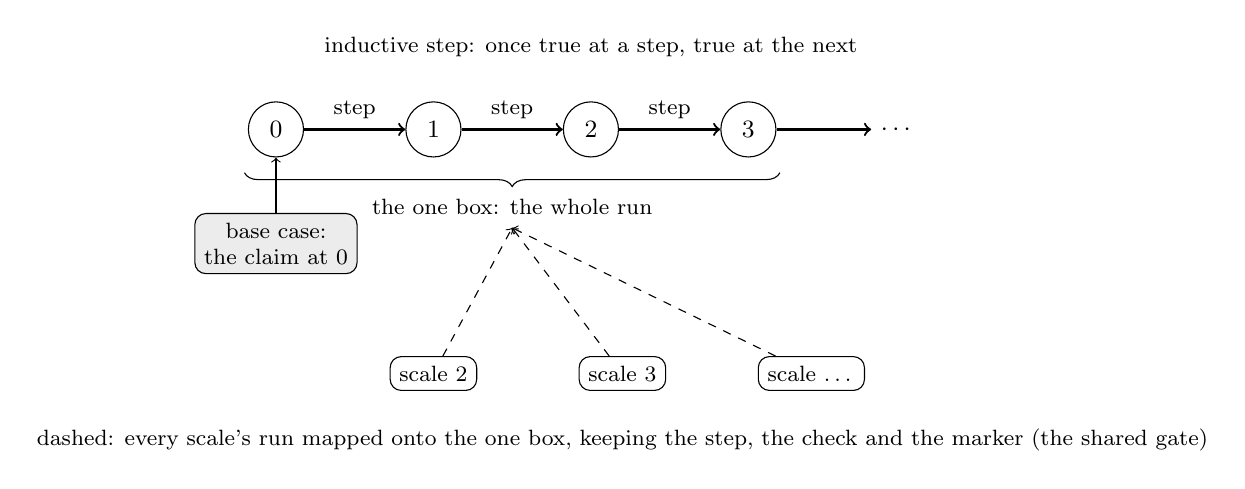
\begin{tikzpicture}[x=1cm,y=1cm,every node/.style={font=\small}]
  \foreach \i in {0,1,2,3} { \node[draw,circle,minimum size=7mm] (s\i) at (\i*2,0) {$\i$}; }
  \node (dots) at (7.9,0) {$\cdots$};
  \foreach \i/\j in {0/1,1/2,2/3} { \draw[->,thick] (s\i) -- node[above,font=\footnotesize] {step} (s\j); }
  \draw[->,thick] (s3) -- (dots);
  \node[draw,rounded corners,fill=gray!15,align=center,font=\footnotesize] (base) at (0,-1.45) {base case:\\ the claim at 0};
  \draw[->] (base) -- (s0);
  \node[align=center,font=\footnotesize] at (4,1.05) {inductive step: once true at a step, true at the next};
  \draw[decorate,decoration={brace,mirror,amplitude=5pt}] (-0.4,-0.55) -- (6.4,-0.55) node[midway,below=6pt,font=\footnotesize] (onebox) {the one box: the whole run};
  \node[draw,rounded corners,font=\footnotesize] (c1) at (2,-3.1) {scale 2};
  \node[draw,rounded corners,font=\footnotesize] (c2) at (4.4,-3.1) {scale 3};
  \node[draw,rounded corners,font=\footnotesize] (c3) at (6.8,-3.1) {scale $\dots$};
  \foreach \c in {c1,c2,c3} { \draw[->,dashed] (\c) -- (3,-1.25); }
  \node[align=center,font=\footnotesize] at (4.4,-3.95) {dashed: every scale's run mapped onto the one box, keeping the step, the check and the marker (the shared gate)};
\end{tikzpicture}
\caption{The headline as a picture. A statement is checked at every step of a run; a proof is a base case and an inductive step, and
the dashed maps carry it from the one box to every scale. Where the open part sits: on a card, the base case; on the Yang-Mills box, the
inductive step; for G2, the dashed maps (the shared gate, named R136a1). In the verify toy the content sits in the dashed maps too, and
everything there is proved.}
\end{figure}

\subsection*{II.5 The API: cards}
\addcontentsline{toc}{subsection}{II.5 The API: cards}

\textbf{Why it clicks.} The form layer says nothing about content, so every problem can use it. Every problem has the same shape: an input, a proved structure, one named open step.

\textbf{What the API gives (\href{https://github.com/StevenHrovat/gravity/blob/43a0bd8/docs/paper/D5/CLAIMS.md}{II.5.1}).} One import, \texttt{ProofPhase.\allowbreak{}API}, a facade over the form layer: it moves and renames nothing, and its theorems are re-exports or one-line wrappers. It has one structure per concept \textbf{[Lean]} (\texttt{API.lean}):

{\footnotesize
\begin{longtable}{>{\raggedright\arraybackslash}p{\dimexpr 0.2080\linewidth-2\tabcolsep\relax}>{\raggedright\arraybackslash}p{\dimexpr 0.2246\linewidth-2\tabcolsep\relax}>{\raggedright\arraybackslash}p{\dimexpr 0.2493\linewidth-2\tabcolsep\relax}>{\raggedright\arraybackslash}p{\dimexpr 0.2982\linewidth-2\tabcolsep\relax}}
\toprule
\textbf{Concept} & \textbf{In Lean} & \textbf{You supply} & \textbf{You get for free} \\
\midrule
\endhead
a running system & \texttt{RunSys} & states, step, factor, mass, the ledger law & \texttt{carry}, \texttt{contract}, \texttt{decay\_cost} \\
the settle bound & \texttt{settle}, \texttt{settle\_\allowbreak{}everywhere}, \texttt{settle\_\allowbreak{}iff\_\allowbreak{}bounded}, \texttt{balanceBound} & the contraction class & an explicit step count \\
the decidability edge & \texttt{edge} & nothing & decided above the floor, undecidable at it \\
a chain with costs & \texttt{Chain} & a quantity, costs, the step law & \texttt{Chain.\allowbreak{}ledger}, \texttt{Chain.decay}, \texttt{Chain.\allowbreak{}summable}, \texttt{Chain.size} \\
a margin that survives & \texttt{Margin} & shares kept & \texttt{Margin.\allowbreak{}survive}, \texttt{Margin.pos} \\
an encoder & \texttt{Encoder}, \texttt{szegoFactor}, \texttt{elecFactor}, \texttt{cost} & a state and its rotation & the Szeg\H{o} factor in [0, 1] (\texttt{szegoFactor\_\allowbreak{}mem}); the electric factor is \texttt{elec (Re c)} \\
an uncertainty & \texttt{Uncertainty} & error, factor, fresh uncertainty & \texttt{bounded}, \texttt{critical}, \texttt{sign} \\
the problem card & \texttt{Problem} & input, \texttt{Open}, \texttt{Concl}, \texttt{proved} & \texttt{Problem.\allowbreak{}holds} \\
the open-step slot & \texttt{OpenStep "name" P} & the one statement \texttt{P} & \texttt{P} itself, labelled \\
the external-input slot & \texttt{External "source" P} & a theorem from the literature & \texttt{P} itself, labelled \\
\bottomrule
\end{longtable}}

The slots are transparent: \texttt{OpenStep ".\allowbreak{}.\allowbreak{}.\allowbreak{}" P} \emph{is} \texttt{P}, so a theorem takes it as an ordinary hypothesis. Nothing is ever an axiom. The labels make the open steps and outside dependencies greppable.

\textbf{Adding a problem (\href{https://github.com/StevenHrovat/gravity/blob/43a0bd8/docs/paper/D5/CLAIMS.md}{II.5.2}).} Seven steps: copy the template (\texttt{API/\allowbreak{}Template.\allowbreak{}lean}, a worked toy); write the input; fill a running system, chain or margin and check the one ledger inequality; write the open step in its slot; call the free theorems; add an uncertainty if the input is only approximate; state the card. \textbf{[paper]} (the procedure; \texttt{docs/\allowbreak{}unified/\allowbreak{}API.\allowbreak{}md}, 3). The three cards of Parts III to V are \texttt{API/\allowbreak{}YangMills.\allowbreak{}lean}, \texttt{API/\allowbreak{}GRH.\allowbreak{}lean} and \texttt{API/NP.lean}, each proved as ``open step gives conclusion'' \textbf{[Lean]}; each open step is \textbf{[open]} (\href{https://github.com/StevenHrovat/gravity/blob/43a0bd8/docs/paper/D5/CLAIMS.md}{III.5.6}, IV.4, V.6: \texttt{CrossingCost}, with \href{https://github.com/StevenHrovat/gravity/blob/43a0bd8/docs/paper/D5/CLAIMS.md}{V.4.10} the nearest concrete target). A problem may have several cards: Navier-Stokes has three (VI.2), BSD three (VII.2), Hodge five (VIII.2); GU has a box and no card (IX.2). The GRH card is a card for a finite model of zeros (its open step \texttt{ScaleSign} is the sign at every scale of that model); the link to zeta is \texttt{tie\_in}, which takes the statement of the Riemann hypothesis as an \texttt{External} hypothesis. The toy settles in 101 steps to 1/100 (\texttt{toy\_\allowbreak{}settle\_\allowbreak{}101}) \textbf{[Lean]}.

\textbf{What runs and what is truth only (\href{https://github.com/StevenHrovat/gravity/blob/43a0bd8/docs/paper/D5/CLAIMS.md}{II.5.3}).} The settle count, the encoder factors on rational data and the ledger law on rational data are computable and decidable: \texttt{balanceBound}, \texttt{szegoQ}, \texttt{elecQ}, \texttt{PaysQ}, \texttt{settle0}, with \texttt{szegoQ\_\allowbreak{}cast}, \texttt{elecQ\_cast} and \texttt{PaysQ.pays} proving them right for the real system; the machine's step and balance test are primitive recursive (\texttt{estep\_\allowbreak{}primrec}, \texttt{halted\_\allowbreak{}primrec}). The real-valued structures and the undecidability on the lossless side are truth statements, not computed. \textbf{[Lean]} (\texttt{API.lean}).

\textbf{One consequence for every instance (\href{https://github.com/StevenHrovat/gravity/blob/43a0bd8/docs/paper/D5/CLAIMS.md}{II.5.4}).} G0's phase field is one compact circle. Every continuous character of the circle is z -\textgreater{} $z^{n}$ for an integer n, so every label carried on it has integer charge, with no further assumption. \textbf{[Lean]} (\texttt{API/\allowbreak{}Phase.\allowbreak{}lean}, \texttt{chargeQuantisation}, \texttt{PhaseLabel.\allowbreak{}integer\_\allowbreak{}charge}; classical content: Pontryagin duality for the circle).

\textbf{What it does not do (\href{https://github.com/StevenHrovat/gravity/blob/43a0bd8/docs/paper/D5/CLAIMS.md}{II.5.5}).} It proves no open step and adds no mathematics. It does not turn a problem into a running system for you: the structure and its one inequality are the work. Arguments that use only the interface cannot settle P vs NP (relativization, V.7), and the NP card inherits that. \textbf{[paper]}

\medskip\noindent\rule{\linewidth}{0.4pt}\medskip

\subsection*{II.6 The arsenal and its lint}
\addcontentsline{toc}{subsection}{II.6 The arsenal and its lint}

\textbf{Why it clicks.} Content-free results that more than one project uses should live once, and every use should be checkable for one property: that nothing in it cannot run.

\textbf{The arsenal (\href{https://github.com/StevenHrovat/gravity/blob/43a0bd8/docs/paper/D5/CLAIMS.md}{II.6.1}).} The arsenal is the set of transferable Lean results that need Mathlib, kept in the \texttt{im} repository (\texttt{arsenal/}), pinned to Lean and Mathlib v4.34.0. It is imported from there and never copied (\href{https://github.com/StevenHrovat/gravity/blob/43a0bd8/docs/paper/D5/CLAIMS.md}{II.6.4}). At the pinned commit its modules are \texttt{Arsenal.\allowbreak{}R136a1}, \texttt{Arsenal.BSD} with its parts (\texttt{Algebraic}, \texttt{Analytic}, \texttt{Count}, \texttt{Hasse}, \texttt{EulerRat}), \texttt{Arsenal.\allowbreak{}Rotation} (the one-box test, II.4) and \texttt{Arsenal.\allowbreak{}Rigidity} (II.4) \textbf{[paper]} (\texttt{arsenal/\allowbreak{}README.\allowbreak{}md}).

\textbf{R136a1 (\href{https://github.com/StevenHrovat/gravity/blob/43a0bd8/docs/paper/D5/CLAIMS.md}{II.6.2}).} The one way to leave a statement open: \texttt{R136a1 "name" P} is \texttt{P} as a named hypothesis, never an axiom. A theorem that needs it takes it as a hypothesis, so the system never assumes it. \textbf{[Lean]} (\texttt{Arsenal/\allowbreak{}R136a1.\allowbreak{}lean}, \texttt{R136a1}, \texttt{R136a1.out}).

\textbf{The lint (\href{https://github.com/StevenHrovat/gravity/blob/43a0bd8/docs/paper/D5/CLAIMS.md}{II.6.3}).} \texttt{arsenal/\allowbreak{}tools/\allowbreak{}lint.\allowbreak{}sh} is static, needs no network and no build. It fails unless: the toolchain is Lean v4.34.0 and the one requirement is Mathlib at tag v4.34.0; every module imports only Mathlib or the arsenal itself; no module uses an escape hatch (\texttt{sorry}, \texttt{admit}, \texttt{axiom}, \texttt{native\_\allowbreak{}decide}, \texttt{unsafe}, \texttt{implemented\_\allowbreak{}by}, \texttt{extern}, \texttt{ofReduceBool}, \texttt{skipKernelTC}), read in code only so prose stays free; and every module is reached from \texttt{Arsenal.\allowbreak{}lean}. It lists every part answered R136a1 by name. \textbf{[paper]} (read from the script; run at the commit of \texttt{im} pinned in \texttt{docs/\allowbreak{}mass-gap/\allowbreak{}formal/\allowbreak{}lakefile.\allowbreak{}toml}, result ``lint: OK (10 modules; Mathlib v4.34.0 only; no escape hatch; 4 part(s) answered R136a1)'', the four being \texttt{Euler product bound}, \texttt{Hasse}, \texttt{the gate is shared across scales} and \texttt{weak Mordell-Weil}). A self-test (\texttt{tools/\allowbreak{}lint-selftest.\allowbreak{}sh}) plants one case per rule, and the full check (\texttt{tools/\allowbreak{}check.\allowbreak{}sh}) adds a build against Mathlib and the kernel's axiom report for every declaration; both were run at the release commit (II.7).

\textbf{Shared vocabulary, imported and never copied (\href{https://github.com/StevenHrovat/gravity/blob/43a0bd8/docs/paper/D5/CLAIMS.md}{II.6.4}).} What can be transferred moves to the \texttt{im} repository and is used from there as a dependency, never vendored. Lean projects \texttt{require} the package by repository, subdirectory and commit. \textbf{[paper]} (the first author's rule; \texttt{arsenal/\allowbreak{}README.\allowbreak{}md}, ``Using it'').

\textbf{What the lint is, and is not.} It certifies form: that everything stated is soundly constructed. It does not say that the statements describe the world (Part I, R.1).

\medskip\noindent\rule{\linewidth}{0.4pt}\medskip

\subsection*{II.7 The independent re-check}
\addcontentsline{toc}{subsection}{II.7 The independent re-check}

The Lean modules of this paper are checked by kernels other than the one that built them (\texttt{docs/\allowbreak{}unified/\allowbreak{}INDEPENDENT-CHECK.\allowbreak{}md}, \texttt{tools/\allowbreak{}independent-check.\allowbreak{}sh}). Lean's own \texttt{leanchecker} replays each module's declarations into a fresh environment, and \texttt{nanoda\_lib}, a type checker written independently in Rust, checks an export of every declaration together with everything it uses \textbf{[Lean, re-checked]} for the modules a run covered (below). A full run once established a trusted base, Mathlib and Lean core at the pinned commit, recorded by hash in a stamp. Later runs re-check only the modules whose source or imports changed, against that stamp.

\textbf{What the runs covered.} A full run established the trusted base (Mathlib and Lean core at the pinned commit, recorded by hash in \texttt{docs/\allowbreak{}unified/\allowbreak{}independent-check.\allowbreak{}stamp}); quick runs re-check every module changed since, against it. The last quick run covers the source of this paper: \texttt{leanchecker} replayed every changed module with no failure, the axiom audit found no declaration resting on anything beyond \texttt{propext}, \texttt{Quot.sound} and \texttt{Classical.\allowbreak{}choice}, and \texttt{nanoda\_lib} checked the declarations of the changed modules and everything they use with no type-checker error \textbf{[Lean, re-checked]}. IM's arsenal, imported at its pinned commit, is checked like the project's own code and is never part of the trusted base; its own full check passes with 223 declarations on the three standard axioms. The scan for escape hatches reads code only, as the arsenal's lint does, and finds none. Every run, with its commit and numbers, is recorded in \texttt{docs/\allowbreak{}paper/\allowbreak{}REVIEW.\allowbreak{}md} (Record), and \texttt{tools/\allowbreak{}reproduce.\allowbreak{}sh kernels} repeats them (REPRODUCE.md).

\textbf{B. The tools the problems use.}

\subsection*{II.8 One chain, the first three problems}
\addcontentsline{toc}{subsection}{II.8 One chain, the first three problems}

The first three problems (Parts III to V) run along the same four links.

\begin{quote}
\textbf{positivity $\to$ a space $\to$ an evolution on it $\to$ a spectrum that the positivity pins}
\end{quote}

{\footnotesize
\begin{longtable}{>{\raggedright\arraybackslash}p{\dimexpr 0.1642\linewidth-2\tabcolsep\relax}>{\raggedright\arraybackslash}p{\dimexpr 0.2903\linewidth-2\tabcolsep\relax}>{\raggedright\arraybackslash}p{\dimexpr 0.2564\linewidth-2\tabcolsep\relax}>{\raggedright\arraybackslash}p{\dimexpr 0.2692\linewidth-2\tabcolsep\relax}}
\toprule
\textbf{Link} & \textbf{Yang-Mills} & \textbf{GRH} & \textbf{P vs NP (sampling side)} \\
\midrule
\endhead
1. Positivity & reflection positivity of $e^{-S}$ & Weil's pairing W(f * f\textasciitilde{}) $\ge$ 0 & positive weights on assignments \\
2. Space & the Osterwalder-Schrader (OS) Hilbert space & the GNS space of Weil's form & L2 of the Gibbs measure \\
3. Evolution & the transfer matrix $e^{-H}$, H $\ge$ 0 & translation in log-scale & the heat-bath operator, 0 $\le$ P $\le$ 1 \\
4. Spectrum & gap = decay rate of correlations & real spectrum = zeros on the line & gap = fast mixing \\
\bottomrule
\end{longtable}}

\textbf{Why it clicks.} Links 2 to 4 are free once link 1 is given: they are theorems of the same pattern in each column (the reflection step is the Lean form for Yang-Mills, the finite Weil criterion for GRH, the finite spectral measure for the sampling side; II.9 to II.10 give each). The whole difficulty of each problem sits in link 1 for the hard case (Yang-Mills: a certificate at one scale; GRH: positivity itself; P vs NP: the step from a certified class to all inputs). The rest of this part makes links 2 to 4 precise and adds the four tools that act on link 1 or carry it across scales.

\medskip\noindent\rule{\linewidth}{0.4pt}\medskip

\subsection*{II.9 Positivity builds a space}
\addcontentsline{toc}{subsection}{II.9 Positivity builds a space}

\textbf{Why it clicks.} A non-negative form is all you need to measure lengths, and lengths are all you need for a Hilbert space.

\textbf{Theorem \href{https://github.com/StevenHrovat/gravity/blob/43a0bd8/docs/paper/D5/CLAIMS.md}{II.9.1} (reconstruction from a positive form).} Let V be a real or complex vector space with a Hermitian form Q that is positive semi-definite, Q(v, v) $\ge$ 0. Divide out the null vectors and complete: the result is a Hilbert space H with a map $\Phi$ : V $\to$ H such that \textless{}$\Phi$ u, $\Phi$ v\textgreater{} = Q(u, v). A linear map $\tau$ on V that is symmetric for Q and satisfies Q($\tau$ u, $\tau$ u) $\le$ Q(u, u) descends to a bounded self-adjoint operator T on H with 0 \textless{}= \textless{}x, T x\textgreater{} when Q(u, $\tau$ u) $\ge$ 0. \textbf{[classical]} (Gelfand-Naimark-Segal; Osterwalder-Schrader, Commun. Math. Phys. 31 (1973) 83-112 and 42 (1975) 281-305). \textbf{[Lean]} in the abstract form used for Yang-Mills, over the reals (\texttt{RPData}: a symmetric real form, reflection positivity, a symmetric positive step with bounded orbits): \texttt{M1/\allowbreak{}UVTVOS.\allowbreak{}lean} (\texttt{inner\_Φ}, \texttt{T\_symm}, \texttt{T\_pos}, \texttt{contraction}).

\textbf{The three applications.}

\begin{itemize}
\item \textbf{Yang-Mills.} Q(F, G) = \textless{}$\theta$ F, G\textgreater{}, with $\theta$ the time reflection. Reflection positivity of the Wilson action, site and link, is \textbf{[Lean]} (\texttt{docs/\allowbreak{}mass-gap/\allowbreak{}formal/\allowbreak{}Positivity/\allowbreak{}}; the lattice has even extent N in the reflection direction, \texttt{wilson\_rp},
\end{itemize}
\texttt{wilson\_\allowbreak{}rp\_\allowbreak{}SU2}). The transfer step is $\tau$. Positivity is given by construction.

\begin{itemize}
\item \textbf{GRH.} Q is Weil's explicit-formula pairing. In a finite model (finitely many zeros, closed under conjugation) the pairing is non-negative on every finite exponential sum \textbf{iff} every zero is on the line \textbf{[Lean]} (\texttt{GRH/\allowbreak{}Weil.\allowbreak{}lean}, \texttt{weil\_\allowbreak{}criterion\_\allowbreak{}finite}). For the zeta function itself the equivalence is Weil's criterion \textbf{[classical]} (Weil 1952\,\hyperlink{bib215}{[215]}; Bombieri 2000\,\hyperlink{bib27}{[27]}). Positivity is \emph{not} given by construction: it is equivalent to the conclusion.
\item \textbf{P vs NP (sampling).} Q is the L2 inner product of a Gibbs measure with positive weights; the heat-bath operator is self-adjoint and positive, and every time correlation has a spectral measure on [0, 1] \textbf{[Lean]} (\texttt{Mixing/\allowbreak{}FiniteSpectral.\allowbreak{}lean}, \texttt{timeCorr\_\allowbreak{}spectral}).
\end{itemize}
\medskip\noindent\rule{\linewidth}{0.4pt}\medskip

\subsection*{II.10 Positivity pins the spectrum}
\addcontentsline{toc}{subsection}{II.10 Positivity pins the spectrum}

\textbf{Why it clicks.} A self-adjoint operator cannot hide anything off the real axis, and a positive contraction cannot hide anything outside [0, 1]. So ``where is the spectrum'' becomes ``how fast do correlations decay''.

\textbf{Theorem \href{https://github.com/StevenHrovat/gravity/blob/43a0bd8/docs/paper/D5/CLAIMS.md}{II.10.1} (decay rate = bottom of the spectrum).} Let $\nu$ be a finite measure on [0, inf) (the spectral measure of a vector for H $\ge$ 0) and corr(t) = int $e^{-tE}$ d $\nu$(E). Then corr(n) $\le$ K $e^{-mn}$ for all n, for some K, \textbf{iff} $\nu$ gives no mass below m. The admissible decay rates are exactly the m with $\nu$([0, m)) = 0, and the best rate is the bottom of the support. \textbf{[Lean]} (\texttt{Bridge/\allowbreak{}Spectral.\allowbreak{}lean}, \texttt{spectral\_\allowbreak{}gap\_\allowbreak{}iff}, \texttt{decayRates\_\allowbreak{}eq}; discrete-time form \texttt{Mixing/\allowbreak{}TimeGap.\allowbreak{}lean}, \texttt{time\_\allowbreak{}gap\_\allowbreak{}iff}).

\textbf{Corollary \href{https://github.com/StevenHrovat/gravity/blob/43a0bd8/docs/paper/D5/CLAIMS.md}{II.10.2} (gap from reflection positivity).} In the setting of \href{https://github.com/StevenHrovat/gravity/blob/43a0bd8/docs/paper/D5/CLAIMS.md}{II.9.1} (the real form of the Lean data), let Blk be a set of blocks that the step $\tau$ maps into itself, on which every correlation decays at rate m (Q(g, $\tau^{n}$ g) $\le$ $C_{g}$ $e^{-mn}$). Let F be approximated by blocks $f_{k}$ with Q(F - $f_{k}$, F - $f_{k}$) $\le$ $bB_{k}$ + 2 $bA_{k}$ and $bA_{k}$, $bB_{k}$ tending to 0 (the block bounds of the UV-TV round: hypotheses \texttt{hsplit}, \texttt{hA}, \texttt{hB}). Then Q(F, $\tau^{n}$ F) $\le$ $e^{-mn}$ Q(F, F) for all n. \textbf{[Lean]} (\texttt{M1/\allowbreak{}UVTVOS.\allowbreak{}lean}, \texttt{gap\_of\_RP}; \texttt{Bridge/\allowbreak{}OSLink.\allowbreak{}lean}, \texttt{gap\_\allowbreak{}of\_\allowbreak{}RP\_\allowbreak{}spectral}, which starts from a spectral representation of the block correlations instead of the decay). It is the quadratic-form form of "the transfer operator has norm at most $e^{-m}$ off the vacuum"; the identification of the vacuum complement is not part of the Lean statement.

\textbf{The three applications.} Yang-Mills: the mass gap is the decay rate of gauge-invariant correlations. GRH: if the generator of the evolution on Weil's space is self-adjoint, its spectrum is real, which in the variable $\gamma$ = ($\rho$ - 1/2)/i is the statement that the zeros are real; that such a space and generator exist for zeta is the Hilbert-Polya view and is \textbf{[open]} (\href{https://github.com/StevenHrovat/gravity/blob/43a0bd8/docs/paper/D5/CLAIMS.md}{IV.4.1}). P vs NP: a spectral gap of the heat-bath operator is fast mixing, hence polynomial-time sampling \textbf{[classical]} (the standard relation between the gap and the mixing time, through the relaxation time; Levin-Peres-Wilmer, chapter 12; claim \href{https://github.com/StevenHrovat/gravity/blob/43a0bd8/docs/paper/D5/CLAIMS.md}{II.10.3}), finite form \textbf{[Lean]} (\texttt{Mixing/}).

\medskip\noindent\rule{\linewidth}{0.4pt}\medskip

\subsection*{II.11 The bridge lemma: positivity locates singularities}
\addcontentsline{toc}{subsection}{II.11 The bridge lemma: positivity locates singularities}

\textbf{Why it clicks.} A sum of positive terms cannot cancel. So the first place where it blows up must be visible on the real axis, where nothing can cancel.

\textbf{Theorem \href{https://github.com/StevenHrovat/gravity/blob/43a0bd8/docs/paper/D5/CLAIMS.md}{II.11.1} (Pringsheim, extension form).} Let F be holomorphic on Re s $>$ x0, write its Taylor coefficients at real points c $>$ x0 as $F^{n}$(c) = (-1)\textasciicircum{}n M(c, n) with M real, and suppose F agrees on the right of x0 with a function holomorphic on a disc about x0. Then for some real c $>$ x0 and h $\ge$ 0 with c - h $<$ x0, the series sum M(c, n) $h^{n}$ / n! converges. \textbf{[Lean]} (\texttt{Bridge/\allowbreak{}Pringsheim.\allowbreak{}lean}, \texttt{pringsheim\_\allowbreak{}extension}; the disc form \texttt{pringsheim\_\allowbreak{}hasSum}). Not in Mathlib before this project.

The Lean core needs no sign: it is Cauchy's theorem in Taylor form. \textbf{Positivity enters in the instances.} There M(c, n) is itself a sum or integral of non-negative terms, such as sum\_k $a_{k}$ (log k)\textasciicircum{}n $k^{-c}$ with $a_{k}$ $\ge$ 0. Non-negative double series may be summed in either order (Tonelli), and the inner sum is the original series evaluated at c - h. So the original series converges beyond the point where it was supposed to stop, a contradiction. That is the whole mechanism: without positivity the reordering fails and a singularity can hide off the real axis.

\textbf{Three instances, all [Lean]:}

\begin{enumerate}
\item \textbf{Landau's theorem.} An L-series with non-negative coefficients has a singularity at the real point of its abscissa of absolute convergence (\texttt{Bridge/\allowbreak{}Landau.\allowbreak{}lean}, \texttt{landau}). The same theorem is the endgame of the proof of RH in Lean by others, which this project read and did not rebuild \textbf{[external]} (IV.0).
\item \textbf{Laplace transforms of positive measures.} For a measure on [0, inf), the real edge of convergence of int $e^{-st}$ d $\mu$ is a singularity (\texttt{Bridge/\allowbreak{}Laplace.\allowbreak{}lean}, \texttt{laplace\_\allowbreak{}landau}).
\item \textbf{The mass gap.} The Laplace integral of the correlation measure of F (a finite measure on [0, inf), the spectral measure of F for H $\ge$ 0) converges for real s $>$ -l0 and is singular at s = -l0, where l0 is the bottom of the support of that measure (\texttt{Bridge/\allowbreak{}Spectral.\allowbreak{}lean}, \texttt{resolvent\_\allowbreak{}singular}). Its identification with the resolvent \textless{}F, (H + s)\textasciicircum{}\{-1\} F\textgreater{} is \textbf{[classical]}.
\end{enumerate}
\textbf{What the bridge does not give.} It locates the \emph{first} singularity of a positive object. It does not make an object positive. Over function fields, one positive duality (the Hodge index theorem) gives both the axis of the functional equation and the balance point 1/2; over the integers no such positivity is known \textbf{[open]} (\texttt{docs/\allowbreak{}rh-guide/\allowbreak{}bridge/\allowbreak{}BRIDGE.\allowbreak{}md}, section 0; claims \href{https://github.com/StevenHrovat/gravity/blob/43a0bd8/docs/paper/D5/CLAIMS.md}{IV.2.5a} and \href{https://github.com/StevenHrovat/gravity/blob/43a0bd8/docs/paper/D5/CLAIMS.md}{IV.2.5c}).

\medskip\noindent\rule{\linewidth}{0.4pt}\medskip

\subsection*{II.12 Contraction and data processing}
\addcontentsline{toc}{subsection}{II.12 Contraction and data processing}

\textbf{Why it clicks.} A lossy channel can only forget. If it forgets a fixed fraction each step, it forgets geometrically, and a geometric rate is a gap.

\textbf{Definitions.} A stochastic kernel K moves probability distributions. Its contraction coefficient $\eta$(K) is the largest factor by which it shrinks the total-variation distance between two distributions (Dobrushin's coefficient). For a system of sites with local conditional laws, the influence C(x, z) of site z on site x is the largest change in the law at x when only z changes; the column sum of z is sum\_x C(x, z).

\textbf{Theorem \href{https://github.com/StevenHrovat/gravity/blob/43a0bd8/docs/paper/D5/CLAIMS.md}{II.12.1} (data processing, composed).} $\eta$(K) $\le$ 1 for every stochastic kernel, and $\eta$(K L) $\le$ $\eta$(K) $\eta$(L). The same kernel applied n times contracts by $\eta^{n.}$ \textbf{[classical]} (Dobrushin, Theory Probab. Appl. 1 (1956) 65-80; the strong data-processing inequality). \textbf{[Lean]} on finite state spaces (\texttt{Mixing/\allowbreak{}Chain.\allowbreak{}lean}, \texttt{contracts\_\allowbreak{}kchain}, \texttt{contracts\_\allowbreak{}kpow}, \texttt{tv\_\allowbreak{}pushv\_\allowbreak{}kpow\_\allowbreak{}le\_\allowbreak{}pow}).

\textbf{Theorem \href{https://github.com/StevenHrovat/gravity/blob/43a0bd8/docs/paper/D5/CLAIMS.md}{II.12.2} (Doeblin: a quantum per tick).} If K(x, .) $\ge$ $\varepsilon$ $\nu$(.) for every x, then $\eta$(K) $\le$ 1 - $\varepsilon$. \textbf{[Lean]} on finite state spaces (\texttt{Mixing/\allowbreak{}Doeblin.\allowbreak{}lean}, \texttt{contracts\_\allowbreak{}of\_\allowbreak{}doeblin}, \texttt{doeblin\_\allowbreak{}sharp}).

\textbf{Theorem \href{https://github.com/StevenHrovat/gravity/blob/43a0bd8/docs/paper/D5/CLAIMS.md}{II.12.3} (one finite check, decay everywhere).} If every column sum of the influence matrix is at most $\alpha$ $<$ 1, the heat-bath dynamics has a spectral gap: the spectral measure of every time correlation gives no mass above 1 - (1 - $\alpha$)/N, with N the number of sites. The condition is Dobrushin's (Theory Probab. Appl. 13 (1968) 197-224; Dobrushin-Shlosman 1985\,\hyperlink{bib70}{[70]}, uniqueness and decay of correlations); the gap form is known in the literature on rapid mixing under Dobrushin's condition (Dyer-Goldberg-Jerrum, Combin. Probab. Comput. 17 (2008) 761-779, states the mixing result; Hayes 2006 gives rapid mixing from a Dobrushin matrix of norm below 1; Wu 2006\,\hyperlink{bib221}{[221]} gives the Poincar\'e inequality, a spectral gap, under Dobrushin's uniqueness condition) (claim \href{https://github.com/StevenHrovat/gravity/blob/43a0bd8/docs/paper/D5/CLAIMS.md}{II.12.3}). \textbf{[Lean]} for finitely many sites with finite spin spaces (\texttt{Mixing/\allowbreak{}FiniteSpectral.\allowbreak{}lean}, \texttt{spectral\_\allowbreak{}gap\_\allowbreak{}dobrushin}; \texttt{Mixing/\allowbreak{}Link.\allowbreak{}lean}, \texttt{spectral\_\allowbreak{}gap\_\allowbreak{}of\_\allowbreak{}column}). With exponential weights the same condition gives exponential decay of spatial correlations \textbf{[Lean]} (\texttt{docs/\allowbreak{}mass-gap/\allowbreak{}formal/\allowbreak{}Attempts/\allowbreak{}R3/\allowbreak{}TailDecay.\allowbreak{}lean}, \texttt{theoremA\_w}).

\textbf{The honest limit (\href{https://github.com/StevenHrovat/gravity/blob/43a0bd8/docs/paper/D5/CLAIMS.md}{II.12.4}).} Doeblin gives a rate per channel. A site with k $\ge$ 2 neighbours needs the \emph{sum} of the k influences below one, and once the per-channel cost C is at least log 2, the sum of the Doeblin bounds k(1 - $e^{-C}$) is at least 1. The quantum per tick does not by itself give a column below one. \textbf{[Lean]} (\texttt{Mixing/\allowbreak{}Chain.\allowbreak{}lean}, \texttt{column\_\allowbreak{}sum\_\allowbreak{}ge\_\allowbreak{}one}, with the sharp threshold \texttt{column\_\allowbreak{}sum\_\allowbreak{}lt\_\allowbreak{}one\_\allowbreak{}iff}).

\textbf{Uniformity along a chain (\href{https://github.com/StevenHrovat/gravity/blob/43a0bd8/docs/paper/D5/CLAIMS.md}{II.12.5}).} If the same channel acts at every step (a homogeneous chain: translation invariance in the transfer direction), the contraction coefficient is the same at every step; once $\eta$ $<$ 1 at one step, the chain contracts like $\eta^{n.}$ \textbf{[classical]} with the composition law \textbf{[Lean]} above. Read as DMP: ``the uniformity is given by the arrow of causality'' \textbf{[reading]}.

\textbf{The three applications.} Yang-Mills: the gap mechanism reduces to one box of fixed physical size, uniformly over outsides; for a grid the per-box cost must beat the path entropy, $F_{e}$(L) $>$ log $\mu_{4}$ (Part III.5). P vs NP: a column sum below one is polynomial-time sampling and, classically, counting (Part V). GRH: no contraction step is known; the prime-by-prime extension has no slack to lose (Part IV).

\medskip\noindent\rule{\linewidth}{0.4pt}\medskip

\subsection*{II.13 A strict sign gives a rate: the self-dual point}
\addcontentsline{toc}{subsection}{II.13 A strict sign gives a rate: the self-dual point}

\textbf{Why it clicks.} If two quantities are dual to each other and the duality has a fixed point, then they cannot both be small: one of them is at least the fixed-point value.

\textbf{Theorem \href{https://github.com/StevenHrovat/gravity/blob/43a0bd8/docs/paper/D5/CLAIMS.md}{II.13.1} (hand-over).} For 0 $<$ $Z_{tw}$ $<$ Z put $F_{tw}$ = -log($Z_{tw}$ / Z) and $F_{e}$ = -log((Z - $Z_{tw}$)/(Z + $Z_{tw}$)). Then $F_{e}$ is the image of $F_{tw}$ under a decreasing involution with fixed point log(1 + $\sqrt{2}$), and

max($F_{tw}$, $F_{e}$) $\ge$ log(1 + $\sqrt{2}$), about 0.881.

The bound is sharp, attained at $Z_{tw}$ / Z = $\sqrt{2}$ - 1, where both free energies equal log(1 + $\sqrt{2}$) (from \texttt{elec\_\allowbreak{}selfdual} and \texttt{selfdual\_\allowbreak{}cost}, \href{https://github.com/StevenHrovat/gravity/blob/43a0bd8/docs/paper/D5/CLAIMS.md}{II.2.4}; no single theorem states the F-form). \textbf{[Lean]} (\texttt{Crossover/\allowbreak{}HandOver.\allowbreak{}lean}, \texttt{handover\_\allowbreak{}ratio}, \texttt{log\_\allowbreak{}one\_\allowbreak{}add\_\allowbreak{}sqrt\_\allowbreak{}two\_\allowbreak{}le\_\allowbreak{}max}; the duality \texttt{Flip/\allowbreak{}Floor.\allowbreak{}lean}, \texttt{elecF\_\allowbreak{}eq\_\allowbreak{}dual}).

\textbf{Theorem \href{https://github.com/StevenHrovat/gravity/blob/43a0bd8/docs/paper/D5/CLAIMS.md}{II.13.3} (the balance of the full turn).} Let z be positive on N $\ge$ 2 points and $\varepsilon$ positive on N points, tied by the two identities one turn gives: the values of $\varepsilon$ add up to z at the base point, and N times $\varepsilon$ at the base point is the sum of the values of z. Then some nontrivial value of z or of $\varepsilon$ is at most 1/(1 + sqrt N) of its base value, so some nontrivial free energy is at least log(1 + sqrt N) \textbf{[Lean]} (IM, \texttt{Arsenal/\allowbreak{}FullTurn.\allowbreak{}lean}, \texttt{full\_\allowbreak{}turn\_\allowbreak{}balance}, \texttt{full\_\allowbreak{}turn\_\allowbreak{}balance\_\allowbreak{}log}). At N = 2 it is Theorem \href{https://github.com/StevenHrovat/gravity/blob/43a0bd8/docs/paper/D5/CLAIMS.md}{II.13.1}. The bound is sharp: with every nontrivial twist ratio equal to x, the electric ratio is (1 - x)/(1 + (N - 1) x), and the two meet at x = 1/(1 + sqrt N), the self-dual point of the N-step turn \textbf{[paper]} (elementary algebra) (claim \href{https://github.com/StevenHrovat/gravity/blob/43a0bd8/docs/paper/D5/CLAIMS.md}{II.13.3}).

\textbf{Theorem \href{https://github.com/StevenHrovat/gravity/blob/43a0bd8/docs/paper/D5/CLAIMS.md}{II.13.4} (the balance along a path).} Under the same identities the bound holds for the mean free energy over all nontrivial values of one type, not only for their maximum \textbf{[Lean]} (\texttt{full\_\allowbreak{}turn\_\allowbreak{}balance\_\allowbreak{}mean}, by the concavity of the logarithm). So the maximum over sectors is a rate along a path that turns once through the sectors, the base point left out. This is the first author's refinement, ``a maximum over sectors is a rotation of a rate along a path up to the shared root'' \textbf{[reading]}, exact in this form, the shared root being the base point that every sector is measured against (claim \href{https://github.com/StevenHrovat/gravity/blob/43a0bd8/docs/paper/D5/CLAIMS.md}{II.13.4}).

\textbf{Where it applies.} Any system with a strict inequality between a sector and its twist. In SU(2) Yang-Mills the strict inequality holds at every coupling $\beta$ $\ne$ 0 (\texttt{Flip/\allowbreak{}Strict.\allowbreak{}lean}, \texttt{su2\_\allowbreak{}Ztw\_\allowbreak{}lt\_\allowbreak{}Z}), so every periodic SU(2) box with even time extent has a hand-over rate of at least 0.881 nats in one of its two channels, given 0 $<$ $Z_{tw}$ \textbf{[Lean]} (\texttt{Crossover/\allowbreak{}HandOver.\allowbreak{}lean}, \texttt{su2\_\allowbreak{}handover}, with the hypothesis 0 $<$ $Z_{tw}$ stated; the integrand is positive, the formal step is not written). Reading: this is the precise form of I.7, ``existence = non-existence + 1'': a sign with no rate becomes a rate at the self-dual point \textbf{[reading]}.

\textbf{What it does not give.} It is a statement about free energies of the whole periodic box (averaged over everything), not about the influence of an arbitrary fixed outside on one box. And 0.881 suffices for a chain of boxes (two channels per box) but not for a grid: in d $\ge$ 3 the number of ways a path can continue outweighs it (\texttt{Crossover/\allowbreak{}Containment.\allowbreak{}lean}, \texttt{path\_\allowbreak{}entropy\_\allowbreak{}beats\_\allowbreak{}handover}, \textbf{[Lean]}). Both gaps are named in Part III (III.4, III.5).

\medskip\noindent\rule{\linewidth}{0.4pt}\medskip

\subsection*{II.14 The dichotomy: local, crossing flux, residue}
\addcontentsline{toc}{subsection}{II.14 The dichotomy: local, crossing flux, residue}

\textbf{Why it clicks.} An obstruction to decay can only be of three kinds: short-range (it is forgotten), conserved (it cannot be forgotten, so it must be paid for), or stuck inside one region (then it is a finite question about that region).

\textbf{Statement (\href{https://github.com/StevenHrovat/gravity/blob/43a0bd8/docs/paper/D5/CLAIMS.md}{II.14.1}, the shape).} For a system split into regions, every piece of an obstruction is

\begin{itemize}
\item (a) \textbf{local}: forced by a few constraints; behind a collar of positive conditional mass it enters only as a boundary term;
\item (b) \textbf{a crossing flux}: carried by a conserved quantity through the region's boundary; it cannot be screened;
\item (c) \textbf{a residue}: inside one region; what remains is a percolation question: does the bad set span the region, or does it break into finite clusters with an exponential tail?
\end{itemize}
This is a proof strategy, not a theorem \textbf{[paper]} (\texttt{docs/\allowbreak{}mass-gap/\allowbreak{}weak-coupling/\allowbreak{}proof-phase/\allowbreak{}c9a-crossover/\allowbreak{}DICHOTOMY.\allowbreak{}md}; \texttt{docs/\allowbreak{}pnp/\allowbreak{}DICHOTOMY-TRANSFER.\allowbreak{}md}). Its exact pieces are theorems:

\begin{itemize}
\item \textbf{Gauss law mod 2.} For a $Z_{2}$ flux on a graph, the parity crossing the boundary of any region equals the charge inside, whatever the interior does; odd total charge is a contradiction \textbf{[Lean]} (\texttt{Proof/\allowbreak{}Crossing.\allowbreak{}lean}, \texttt{gauss}, \texttt{flux\_fixed}, \texttt{unsat\_\allowbreak{}of\_\allowbreak{}odd}). The same law for centre sheets: a flux-carrying outside forces at least one sheet through the box, entering and leaving an even number of times (when every plaquette lies in an even number of cells) \textbf{[Lean]} (\texttt{Crossover/\allowbreak{}FluxRate.\allowbreak{}lean}, \texttt{exists\_\allowbreak{}sheet\_\allowbreak{}of\_\allowbreak{}flux}, \texttt{even\_\allowbreak{}card\_\allowbreak{}fluxCells}).
\item \textbf{Uncontained pieces weigh nothing.} A sheet that ends inside the box is not a closed configuration, so it has weight zero under every law carried by closed configurations \textbf{[Lean]} (\texttt{Crossover/\allowbreak{}Dichotomy.\allowbreak{}lean}, \texttt{not\_\allowbreak{}uncontained}, \texttt{measure\_\allowbreak{}uncontained}).
\item \textbf{Every refutation crosses.} In every sound proof system whose rules have at most two premises, every refutation of an expanding formula contains a line sensitive to at least the expansion many variables, where ``expanding'' is two stated hypotheses (every proper subset of the blocks is satisfiable; boundary expansion for the middle sizes: each boundary variable makes its one block of the region true wherever that block is false, and the region's other blocks do not contain it) \textbf{[Lean]} (\texttt{Proof/\allowbreak{}Crossing.\allowbreak{}lean}, \texttt{cross\_\allowbreak{}any\_\allowbreak{}system\_\allowbreak{}of\_\allowbreak{}falsify}). For clause blocks both conditions hold whenever the variable occurs in exactly one clause of the region (\texttt{fixes\_\allowbreak{}of\_\allowbreak{}single}, \texttt{invisible\_\allowbreak{}of\_\allowbreak{}not\_\allowbreak{}mem}), so the theorem covers CNF formulas with unique-neighbour expansion; for parity blocks it is \texttt{Tseitin.\allowbreak{}cross\_\allowbreak{}any\_\allowbreak{}system}. The argument is the measure argument of Ben-Sasson and Wigderson, machine-checked for every sound two-premise system.
\item \textbf{Rarity and saturation do not overlap.} The regime where sheets are suppressed (their cost beats their entropy) and the regime where they saturate are disjoint (with entropy K' \textgreater{}= 2(d - 1) and $E_{min}$ $\le$ E, both cannot hold) \textbf{[Lean]} (\texttt{Crossover/\allowbreak{}Dichotomy.\allowbreak{}lean}, \texttt{window\_gap}); that a route between them crosses a window where neither mechanism applies is the consequence read off this.
\end{itemize}
\textbf{The three applications.} Yang-Mills: (b) is exact, (a) fails uniformly at the SO(3) cut, (c) is the open window (Part III). P vs NP: the crossing is universal, but its \emph{cost}, the price of naming the conserved quantity in the system's lines, is not; that cost is the open lower bound (Part V). GRH: the analogue of (b) is the zeros on the line, ``pure oscillation'' \textbf{[reading]}; no dichotomy proof exists there.

\medskip\noindent\rule{\linewidth}{0.4pt}\medskip

\subsection*{II.15 The native optimization method}
\addcontentsline{toc}{subsection}{II.15 The native optimization method}

\textbf{Why it clicks.} A cost that comes in whole units cannot fall forever. Lower it by one unit per improving pass and the method must stop, at an irreducible core.

\textbf{Theorem \href{https://github.com/StevenHrovat/gravity/blob/43a0bd8/docs/paper/D5/CLAIMS.md}{II.15.1} (quantized descent arrives).} Let f be a map on any set and $\mu$ a natural-number measure with $\mu$(f x) $<$ $\mu$(x) whenever f x $\ne$ x. Then f has a fixed point after at most $\mu$(x) steps from x. \textbf{[Lean]} (\texttt{Native/\allowbreak{}Method.\allowbreak{}lean}, \texttt{fixed\_\allowbreak{}after}, \texttt{reaches\_\allowbreak{}floor}). Without quanta it fails: x $\to$ (x + 1)/2 strictly decreases toward 1 and never reaches it (\texttt{real\_\allowbreak{}never\_\allowbreak{}arrives}).

\textbf{Theorem \href{https://github.com/StevenHrovat/gravity/blob/43a0bd8/docs/paper/D5/CLAIMS.md}{II.15.2} (a true contraction for depth).} Pairwise merging of adjacent layers turns d layers into ceil(d/2); after ceil(log2 d) passes one layer remains. \textbf{[Lean]} (\texttt{Native/\allowbreak{}Method.\allowbreak{}lean}, \texttt{iterate\_\allowbreak{}clog\_\allowbreak{}pairUp}).

\textbf{Measured.} Applied to this project's own proof chains, the per-layer kernel cost is finite and bounded by the size of the finite building blocks it evaluates (0.17 to 1.4 ms per layer in the deepest DMP chain; about 0.3 ms per recipe line for a reflected check). \textbf{[numerical]} (\texttt{docs/\allowbreak{}pnp/\allowbreak{}NATIVE-METHOD.\allowbreak{}md}, section 0).

\textbf{The three applications.} P vs NP: the method reduces any refutation to an irreducible core; whether that core is always of polynomial size is the open question N1 (Part V). Yang-Mills: the same ``quantum, then arrival'' shape is the Doeblin rate per tick (\href{https://github.com/StevenHrovat/gravity/blob/43a0bd8/docs/paper/D5/CLAIMS.md}{II.12.2}). GRH: the integer multiplicities of zeros and prime powers are the quanta on the prime side \textbf{[reading]}.

\medskip\noindent\rule{\linewidth}{0.4pt}\medskip

\subsection*{II.16 What the tools do not do}
\addcontentsline{toc}{subsection}{II.16 What the tools do not do}

None of II.9 to II.15 creates positivity. Each starts from a positive weight, a positive pairing, a positive cost or a strict sign, and carries it: into a space, into a spectrum, across a chain, across a boundary, down to a floor. The open step of each problem is the place where that starting positivity is known locally, or in a model, and must be established for every case. Part X states this once (section 4). The six sections II.1 to II.6 are the \emph{form layer}: the part of the machinery that says nothing about content and so serves every problem. II.16 holds for them too.

\medskip\noindent\rule{\linewidth}{0.4pt}\medskip

\subsection*{II.17 Where Part II ends}
\addcontentsline{toc}{subsection}{II.17 Where Part II ends}

The tools II.9 to II.15 carry a positivity. The form layer II.1 to II.6 carries a certificate and its uncertainty, says when the carrying settles, and says where the one open statement of a problem goes. None of it supplies a positivity, and none supplies a floor. Part X says why each problem's open step stays open.


%% ---- 03-part-III-yang-mills.md
\section*{Part III. Yang-Mills: the gap mechanism reduces to one box of fixed physical size}
\addcontentsline{toc}{section}{Part III. Yang-Mills: the gap mechanism reduces to one box of fixed physical size}

\textbf{As a statement checked step by step (II.4.1).} The steps are the lattice levels from a first level k0 of one box of fixed physical size; the statement checked at each level is the level criterion, the box's best one-box ratio within the margin. For some cell geometry and margin this holds at every level exactly when O1 holds in its Lean form \textbf{[Lean]} (\texttt{FineOneBox}, \texttt{fineOneBox\_\allowbreak{}iff\_\allowbreak{}complete}, III.12). Here the inductive step, from each level to the next, carries the content; the split into the first level and the step is exact (\texttt{route\_iff}), not a method of proof. The card's own box (\texttt{YMOneBox}) checks the chain form at every step, so there the open part is the base case.

\subsection*{III.0 What is proved and what is not}
\addcontentsline{toc}{subsection}{III.0 What is proved and what is not}

\textbf{The Clay statement} (Jaffe-Witten, official problem description): for every compact simple gauge group G, a non-trivial quantum Yang-Mills theory exists on $R^{4}$ and has a mass gap $\Delta$ $>$ 0, that is, the Hamiltonian has no spectrum in (0, $\Delta$). Existence includes axiomatic properties at least as strong as the Wightman and Osterwalder-Schrader axioms, with local gauge-invariant fields; the description also asks that the short-distance correlation functions of those fields agree with asymptotic freedom and perturbative renormalisation.

\textbf{This part does not prove it.} For SU(2) it proves two things.

\begin{enumerate}
\item \textbf{The minting half} (I.5): from a gap certificate at one box scale to the mass gap of the lattice theory in both orders of limits, with reflection positivity of the limit \textbf{[Lean]}, conditional on stated inputs (III.2). The Lean gap is a decay statement for slab correlations of bounded physical extent along a tuning; the step to a gap of the Hamiltonian on a Hilbert space is \href{https://github.com/StevenHrovat/gravity/blob/43a0bd8/docs/paper/D5/CLAIMS.md}{III.2.7} (\textbf{[paper]}).
\item \textbf{The global structure of the pressing half}: a per-box rate in one of two channels, a conserved carrier that no collar can screen, superadditivity along a chain, uniformity along it, and the conversion to physical units. Together they reduce the \textbf{gap mechanism} to one statement about one box \textbf{[Lean]} + \textbf{[classical]} (III.3). Sections III.4 and III.5 show why that box statement is harder for a grid of boxes than for a chain, and sharpen it to one number.
\end{enumerate}
It leaves four things open.

\begin{itemize}
\item \textbf{(O1) The one-box statement} (\href{https://github.com/StevenHrovat/gravity/blob/43a0bd8/docs/paper/D5/CLAIMS.md}{III.5.6}). In its Lean form O1 is \texttt{FineOneBox} (\href{https://github.com/StevenHrovat/gravity/blob/43a0bd8/docs/paper/D5/CLAIMS.md}{III.5.9}): one box of fixed physical size whose influence bounds, under every boundary condition, satisfy a one-box sum below one, uniformly in level and volume. The number attached to it is path counting (\textbf{[paper]}, \href{https://github.com/StevenHrovat/gravity/blob/43a0bd8/docs/paper/D5/CLAIMS.md}{III.5.9}): the electric flux free energy must exceed the path entropy of the four-dimensional lattice after the neutral excess act, \textbf{$F_{e}$(L) - 2C $>$ log $\mu_{4}$ = 1.91}, with C a bound on the excess act c(L) on every multiple of L (III.3, \href{https://github.com/StevenHrovat/gravity/blob/43a0bd8/docs/paper/D5/CLAIMS.md}{III.5.8}). That is a sufficient route to the one-box sum, not a necessary one, and $F_{e}$(L) in it is the torus free energy of III.3; ``uniformly over every well-defined outside'' is the content of the Lean form, and for the number it is a heuristic (\href{https://github.com/StevenHrovat/gravity/blob/43a0bd8/docs/paper/D5/CLAIMS.md}{III.5.7}). As E = $mc^{2}$ is $E^{2}$ = (pc)\textasciicircum{}2 + ($mc^{2}$)\textasciicircum{}2 with the momentum term dropped (a \textbf{[reading]}), the familiar form drops the excess act and reads $F_{e}$(L) $>$ 1.91 (twist ratio r(L) $>$ 0.74); it is weaker and alone does not give the chain (\href{https://github.com/StevenHrovat/gravity/blob/43a0bd8/docs/paper/D5/CLAIMS.md}{III.5.8}). In effective-string units the familiar form asks for a box of side L $\sqrt{\sigma}$ of about 1.7 to 1.8 (III.7.4, model evaluation, \textbf{[numerical]}); the full form asks for at least that.
\item \textbf{(O2) The identification inputs}: the line of constant physics (OnLCP) and non-triviality, the two hypotheses that make the lattice family Yang-Mills and not some other gapped family (III.9). The gap itself needs of the line of constant physics only its resolution clause (\href{https://github.com/StevenHrovat/gravity/blob/43a0bd8/docs/paper/D5/CLAIMS.md}{III.9.5}, \textbf{[Lean]}). Per box, the reflected correlation at even time is a reflection-positivity square, hence non-negative for observables of the positive half (\href{https://github.com/StevenHrovat/gravity/blob/43a0bd8/docs/paper/D5/CLAIMS.md}{III.9.5a}, \textbf{[Lean]}). That is not non-triviality: pure noise has correlation zero and passes it too. Non-triviality needs a scale-uniform lower bound c $>$ 0. That lower edge and the scheme clause (\href{https://github.com/StevenHrovat/gravity/blob/43a0bd8/docs/paper/D5/CLAIMS.md}{III.9.5b}) are what remains; they are the opposite edge to O1's decay, independent of O1 in the spectral model, and \textbf{[open]}. On the first author's reading they are not a second assumption: the ODP ends only at a dimensionless 1, so a running, DMP-complete system carries the lower edge by construction, and \href{https://github.com/StevenHrovat/gravity/blob/43a0bd8/docs/paper/D5/CLAIMS.md}{III.9.5b} is the lower edge of the one assumption, beside O1's upper edge, placed at the ODP's end, the certified start \texttt{\{infinity, 2, 3\}} (Part X 4.4, \href{https://github.com/StevenHrovat/gravity/blob/43a0bd8/docs/paper/D5/CLAIMS.md}{X.64a}, \textbf{[reading]}). Under that reading nothing more is to be shown at the start, and the direction of every later tick is \textbf{[conditional]} on the one assumption (\href{https://github.com/StevenHrovat/gravity/blob/43a0bd8/docs/paper/D5/CLAIMS.md}{X.66}).
\item \textbf{(O3) The continuum field theory}: Euclidean invariance, local fields as distributions, uniqueness of the limit, Wightman reconstruction, and short-distance agreement with asymptotic freedom. The external construction this project uses (III.9: a Lean 4 submission of 28 October 2026 and the hosting group's assessment of 10 November 2026, not refereed) is assessed there, as the assessors' opinion, to give a Wightman theory as a scaling limit of Wilson lattice gauge theory, in a selected phase, along a subsequence in the volume, with fields smeared against tests away from coincident points \textbf{[external]}. Its sources say it does not prove uniqueness of the infinite-volume limit or a mass gap, so uniqueness of the limit is \textbf{[open]} for it as for this project's own objects. For this project's own objects, rotation invariance cannot yet be stated, since the lattice has only the hypercubic group \textbf{[open]}.
\item \textbf{(O4) Other groups}: the Lean setting has a tuning for SU(2) only. The SU(N) package and the audit of what generalises are partial (\texttt{General/}, \texttt{proof-phase/\allowbreak{}GENERALISE-AUDIT.\allowbreak{}md}).
\end{itemize}
The title's ``one box'' is exact for the gap mechanism (O1). It is not true of the Clay statement as a whole, which also needs O2 to O4.

\textbf{Why O1 is one number at one scale.} ``The loss rate of one box is below one'' is not enough: the crossover rounds showed that the per-box rate 0.881 suffices for a chain of boxes but not for a grid (III.4), and that it suffices for a grid exactly when the influence runs in tubes, which needs a larger electric cost per box (III.5). O1 is one statement about one box at one scale.

\textbf{Convention for $\beta$.} In the Lean, $\beta$ = 2/$g^{2}$: the plaquette weight is exp($\beta$ Re tr $U_{p}$) (\texttt{Assembly.\allowbreak{}lean}), and the one-loop slope is 11/(6 $\pi^{2}$). The notes behind III.5.5, III.6 and III.9 (the floor e\textasciicircum{}\{-2 $\beta$ N\}, S $\ge$ $\pi^{2}$ $\beta$ = 4 $\pi^{2}$/$g^{2}$, $\beta_{eff}$ = 4/$g^{2}$ in \texttt{RDOEBLIN.md}) were written with the standard $\beta$ = 4/$g^{2}$, the weight exp(($\beta$/2) tr $U_{p}$). Where this part writes a bare $\beta$ in a formula it says which one. The simulations of III.7 ($\beta$ = 2.3 and 3.5) use the standard $\beta$ = 4/$g^{2}$: their SU(2) heat bath draws each link with weight exp($\beta$ (1/2) tr(U A)) for the staple sum A (Kennedy-Pendleton and Creutz updates; \texttt{proof-phase/\allowbreak{}c9a-crossover/\allowbreak{}w2/\allowbreak{}smalltorus.\allowbreak{}py}, \texttt{sample\_w0}, \texttt{heatbath}) \textbf{[paper]} (read from the code).

\subsection*{III.1 The lattice theory and its positivity (G0 by construction)}
\addcontentsline{toc}{subsection}{III.1 The lattice theory and its positivity (G0 by construction)}

Yang-Mills is the one problem of the first three whose starting positivity is given. The Wilson weight $e^{-S}$ is positive and local, and from those two facts reflection positivity follows. Everything in this section is machine-checked.

{\footnotesize
\begin{longtable}{>{\raggedright\arraybackslash}p{\dimexpr 0.1050\linewidth-2\tabcolsep\relax}>{\raggedright\arraybackslash}p{\dimexpr 0.4047\linewidth-2\tabcolsep\relax}>{\raggedright\arraybackslash}p{\dimexpr 0.1777\linewidth-2\tabcolsep\relax}>{\raggedright\arraybackslash}p{\dimexpr 0.2926\linewidth-2\tabcolsep\relax}}
\toprule
\textbf{\#} & \textbf{Result} & \textbf{Status} & \textbf{Source} \\
\midrule
\endhead
\href{https://github.com/StevenHrovat/gravity/blob/43a0bd8/docs/paper/D5/CLAIMS.md}{III.1.1} & Wilson measure on the 4D torus for SU(2) and general compact G & \textbf{[Lean]} & \texttt{AreaLaw/\allowbreak{}ConcreteSUn.\allowbreak{}lean}, \texttt{OneScale/} \\
III.1.2 & Reflection positivity, site and link & \textbf{[Lean]} & \texttt{Positivity/\allowbreak{}Wilson.\allowbreak{}lean} (\texttt{wilson\_rp}), \texttt{Positivity/\allowbreak{}LinkWilson.\allowbreak{}lean}, \texttt{Positivity/\allowbreak{}Concrete.\allowbreak{}lean} (\texttt{wilson\_\allowbreak{}rp\_\allowbreak{}SU2}) \\
\href{https://github.com/StevenHrovat/gravity/blob/43a0bd8/docs/paper/D5/CLAIMS.md}{III.1.3} & Temporal-gauge transfer kernel; centre flip of one row is a symmetry (\texttt{top\_parity}, any probability space); sector identity $Z_{e}$ = (Z + $Z_{tw}$)/2 (\texttt{twist\_\allowbreak{}centre\_\allowbreak{}transform}, finite configuration spaces; for the SU(2) measure it is the definition of \texttt{elecF}, \texttt{Flip/\allowbreak{}Floor.\allowbreak{}lean}) & \textbf{[Lean]} (identity definitional) & \texttt{Attempts/\allowbreak{}R4/\allowbreak{}LayerKernel.\allowbreak{}lean}, \texttt{LayerSector.\allowbreak{}lean} \\
\href{https://github.com/StevenHrovat/gravity/blob/43a0bd8/docs/paper/D5/CLAIMS.md}{III.1.4} & 't Hooft duality: the lattice rotation maps the temporal twist to the spatial twist on the symmetric box & \textbf{[Lean]} & \texttt{RouteB/\allowbreak{}Duality.\allowbreak{}lean}, \texttt{tHooft\_\allowbreak{}rotation} \\
III.1.5 & A good blocking: centre-covariant and reflection-positive at every level & \textbf{[Lean]}; non-trivial limit at fixed L1 \textbf{[paper]} & \texttt{RouteA/\allowbreak{}Blocking.\allowbreak{}lean}, \texttt{goodBlocking\_\allowbreak{}rp}; \texttt{proof-phase/\allowbreak{}ws1-routeA/\allowbreak{}NOTE.\allowbreak{}md} \\
\href{https://github.com/StevenHrovat/gravity/blob/43a0bd8/docs/paper/D5/CLAIMS.md}{III.1.6} & Strict flip bound $Z_{tw}$ $<$ Z for every $\beta$ $\ne$ 0, every box, every twist position (``existence = non-existence + 1'', I.7) & \textbf{[Lean]} & \texttt{Flip/\allowbreak{}Strict.\allowbreak{}lean}, \texttt{su2\_\allowbreak{}Ztw\_\allowbreak{}lt\_\allowbreak{}Z} \\
\href{https://github.com/StevenHrovat/gravity/blob/43a0bd8/docs/paper/D5/CLAIMS.md}{III.1.7} & The one-step transfer kernel at fixed cross-section is strictly positive & \textbf{[Lean]} & \texttt{Flip/\allowbreak{}Bound.\allowbreak{}lean}, \texttt{stepK\_pos} \\
\bottomrule
\end{longtable}}

\subsection*{III.2 The minting half: from a certificate to the gap}
\addcontentsline{toc}{subsection}{III.2 The minting half: from a certificate to the gap}

Suppose one box, at one scale, is known to forget its outside at a fixed rate. Then the whole lattice theory has a mass gap, in both orders of limits, and the reconstructed Hilbert space carries a transfer operator with a spectral gap. That implication is the minting half, and it is done.

{\footnotesize
\begin{longtable}{>{\raggedright\arraybackslash}p{\dimexpr 0.1056\linewidth-2\tabcolsep\relax}>{\raggedright\arraybackslash}p{\dimexpr 0.4026\linewidth-2\tabcolsep\relax}>{\raggedright\arraybackslash}p{\dimexpr 0.1589\linewidth-2\tabcolsep\relax}>{\raggedright\arraybackslash}p{\dimexpr 0.3129\linewidth-2\tabcolsep\relax}}
\toprule
\textbf{\#} & \textbf{Result} & \textbf{Status} & \textbf{Source} \\
\midrule
\endhead
\href{https://github.com/StevenHrovat/gravity/blob/43a0bd8/docs/paper/D5/CLAIMS.md}{III.2.1} & Dobrushin uniqueness with exponential weights; D' gives decay of block observables at one rate (abstract Gibbs systems) & \textbf{[Lean]} & \texttt{Attempts/\allowbreak{}R3/\allowbreak{}TailDecay.\allowbreak{}lean} (\texttt{theoremA\_w}), \texttt{Attempts/\allowbreak{}R3/\allowbreak{}Robust.\allowbreak{}lean} (\texttt{gap\_\allowbreak{}of\_\allowbreak{}localFactorsW}) \\
\href{https://github.com/StevenHrovat/gravity/blob/43a0bd8/docs/paper/D5/CLAIMS.md}{III.2.2} & Block decay converted to physical units (Corollary B) & \textbf{[Lean]} & \texttt{OneScale/\allowbreak{}CorollaryB.\allowbreak{}lean}, \texttt{corollaryB\_\allowbreak{}lattice} \\
\href{https://github.com/StevenHrovat/gravity/blob/43a0bd8/docs/paper/D5/CLAIMS.md}{III.2.3} & OS route: a windowed block gap gives MassGapLoc and the transfer operator's gap on the reconstructed space & \textbf{[Lean]} & \texttt{OS/\allowbreak{}GapLoc.\allowbreak{}lean} (\texttt{massGapLoc\_\allowbreak{}of\_\allowbreak{}UVTVBlockGap}), \texttt{M1/\allowbreak{}UVTVOS.\allowbreak{}lean} (\texttt{gap\_of\_RP}) \\
\href{https://github.com/StevenHrovat/gravity/blob/43a0bd8/docs/paper/D5/CLAIMS.md}{III.2.4} & The top-level assembly: OpenPieces implies MassGapLoc, LimitRP and NonTrivial (NonTrivial is itself a field of OpenPieces, so it is an output only trivially); reflection positivity of the limit is proved, not assumed & \textbf{[Lean]} & \texttt{Torus/\allowbreak{}Top.\allowbreak{}lean} (\texttt{yang\_\allowbreak{}mills\_\allowbreak{}assembly}), \texttt{Assembly.\allowbreak{}lean} (\texttt{OpenPieces}) \\
\href{https://github.com/StevenHrovat/gravity/blob/43a0bd8/docs/paper/D5/CLAIMS.md}{III.2.5} & The gap in both orders of limits (torus route) & \textbf{[Lean]} & \texttt{Torus/\allowbreak{}Top.\allowbreak{}lean} (\texttt{yang\_\allowbreak{}mills\_\allowbreak{}assembly\_\allowbreak{}torus}); \texttt{Existence/\allowbreak{}Bridge.\allowbreak{}lean} (\texttt{bothOrders\_\allowbreak{}of\_\allowbreak{}torusDecay}) \\
\href{https://github.com/StevenHrovat/gravity/blob/43a0bd8/docs/paper/D5/CLAIMS.md}{III.2.6} & Non-triviality of the hypotheses: pure noise and every bounded coupling fail OpenPieces & \textbf{[Lean]} & \texttt{Assembly.\allowbreak{}lean}, \texttt{not\_\allowbreak{}trivial} \\
\href{https://github.com/StevenHrovat/gravity/blob/43a0bd8/docs/paper/D5/CLAIMS.md}{III.2.7} & MassGapLoc implies a spectral gap of the continuum Hamiltonian (needs density of local vectors and the reconstruction) & \textbf{[paper]}; spectral bridge \textbf{[Lean]} & \texttt{Bridge/\allowbreak{}Spectral.\allowbreak{}lean}, \texttt{Bridge/\allowbreak{}OSLink.\allowbreak{}lean} \\
\href{https://github.com/StevenHrovat/gravity/blob/43a0bd8/docs/paper/D5/CLAIMS.md}{III.2.8} & Strong-coupling gap for any compact group (widest window 18 tanh(n $\beta$) $<$ 1) & \textbf{[Lean]} / \textbf{[paper]} & \texttt{OneScale/\allowbreak{}SingleLink.\allowbreak{}lean} \\
\bottomrule
\end{longtable}}

\textbf{The stated inputs.} \texttt{OpenPieces} (\texttt{Assembly.\allowbreak{}lean}) consists of the line of constant physics \texttt{OnLCP} (resolution, one-loop running, scheme clause), non-triviality \texttt{NonTrivial}, and a route through the crossover (for the torus form \texttt{BlockedTorusRoute}: \texttt{H1Local}, \texttt{LimitDprime}, \texttt{ObsTransferPhys}). In the one-box form (\href{https://github.com/StevenHrovat/gravity/blob/43a0bd8/docs/paper/D5/CLAIMS.md}{III.5.9}) the gap needs only the resolution clause and \texttt{FineOneBox}; \texttt{NonTrivial} and the running and scheme clauses are separate hypotheses that identify the family as Yang-Mills (pure noise also has a gap, \href{https://github.com/StevenHrovat/gravity/blob/43a0bd8/docs/paper/D5/CLAIMS.md}{III.2.6}). \href{https://github.com/StevenHrovat/gravity/blob/43a0bd8/docs/paper/D5/CLAIMS.md}{III.2.7} and III.9 name the rest.

\textbf{The crossover needs no description of its content.} Between the weak-coupling scale $L_{\ast}$ (where M1 controls the law, III.9) and the box scale of O1 lie finitely many blocking steps, each of finite range. The assembly uses only a block gap at one scale; it never needs to know what happens inside the crossover. So the certificate can be checked directly on the actual blocked law at that scale, with no assumption about how the law got there \textbf{[paper]} (\texttt{PREP.md}, ``The crossover is constrained by making no statement about its content''). The price is the quantifier: since nothing is said about the content, the certificate must hold for every content the crossover could have produced, that is, uniformly over every well-defined outside. That quantifier is already part of O1.

\subsection*{III.3 The pressing half: what one box gives, and how a chain carries it}
\addcontentsline{toc}{subsection}{III.3 The pressing half: what one box gives, and how a chain carries it}

This section collects what holds for every box, and what carries it along a line of boxes.

\textbf{A strict sign gives a rate (II.13).} By the strict flip bound (\href{https://github.com/StevenHrovat/gravity/blob/43a0bd8/docs/paper/D5/CLAIMS.md}{III.1.6}) and 't Hooft's duality $F_{e}$ = -log tanh($F_{tw}$/2), at every box size max($F_{tw}$, $F_{e}$) $\ge$ log(1 + $\sqrt{2}$) = 0.881. Rarity's rate is $F_{tw}$, the free energy of a forced centre sheet; disorder's rate is $F_{e}$, the per-box decay of a centre-charged signal. They cannot both be small. \textbf{[Lean]} (\texttt{su2\_\allowbreak{}handover}; hypotheses $\beta$ $\ne$ 0, even time extent, and 0 $<$ $Z_{tw}$). For the SU(N) twisted Wilson partition functions the rate holds with no hypothesis on $Z_{tw}$, for every N $\ge$ 2, every nontrivial sector, $\beta$ $\ne$ 0 and even time extent, since there 0 $<$ $Z_{tw}$ $<$ Z is proved \textbf{[Lean]} (\texttt{General/\allowbreak{}SUNHandOver.\allowbreak{}lean}, \texttt{sun\_\allowbreak{}handover}, from \texttt{sunZtw\_pos}, \texttt{sunZtw\_lt}); that the \texttt{Flip} object of \texttt{su2\_\allowbreak{}handover} is the k = 1 case of that package is the identification \texttt{General/\allowbreak{}SUNTwistInstances.\allowbreak{}lean} names, not proved (claim \href{https://github.com/StevenHrovat/gravity/blob/43a0bd8/docs/paper/D5/CLAIMS.md}{III.3.1b}).

\textbf{All N sectors at once (\href{https://github.com/StevenHrovat/gravity/blob/43a0bd8/docs/paper/D5/CLAIMS.md}{III.3.1c}).} The full turn over the centre $Z_{N}$ (\href{https://github.com/StevenHrovat/gravity/blob/43a0bd8/docs/paper/D5/CLAIMS.md}{II.2.7}) turns the N twisted partition functions into N electric sectors, $Z_{el}$(e) = (1/N) sum over k of cos(2 $\pi$ k e / N) $Z_{tw}$,k, the real form of 't Hooft's electric-flux projection ('t Hooft 1979; real because $Z_{tw}$,-k = $Z_{tw}$,k for even time extent, \texttt{sunZtw\_neg}). One turn gives the sum of the electric sectors as Z and N $Z_{el}$(0) as the sum of the twisted ones, and the balance \href{https://github.com/StevenHrovat/gravity/blob/43a0bd8/docs/paper/D5/CLAIMS.md}{II.13.3} turns these into the rate log(1 + sqrt N): some nontrivial twist free energy or some nontrivial electric free energy of the SU(N) Wilson box is at least log(1 + sqrt N) \textbf{[Lean]}, given that the electric sectors are positive (\texttt{General/\allowbreak{}SUNFullTurn.\allowbreak{}lean}, \texttt{sunZel\_sum}, \texttt{sunZel\_\allowbreak{}zero}, \texttt{sun\_\allowbreak{}handover\_\allowbreak{}full\_\allowbreak{}turn}), and the same holds for the mean over the N - 1 nontrivial sectors of one type (\texttt{sun\_\allowbreak{}handover\_\allowbreak{}full\_\allowbreak{}turn\_\allowbreak{}mean}, \href{https://github.com/StevenHrovat/gravity/blob/43a0bd8/docs/paper/D5/CLAIMS.md}{II.13.4}). For N = 2 the positivity is proved for $\beta$ $\ne$ 0 and even time extent, the sectors being (Z + $Z_{tw}$)/2 and (Z - $Z_{tw}$)/2 (\texttt{sunZel\_\allowbreak{}pos\_\allowbreak{}two}), and the rate is the log(1 + $\sqrt{2}$) above. For N $\ge$ 3 it is a stated hypothesis: each electric sector is the weight of one flux sector of the transfer matrix, positive in the transfer-matrix picture \textbf{[classical]}, not formalised here (claim \href{https://github.com/StevenHrovat/gravity/blob/43a0bd8/docs/paper/D5/CLAIMS.md}{III.3.1c}). The rate grows with N; III.5.4 says what that does and does not give.

\textbf{A flux-carrying outside forces at least one sheet.} The flux cells of a box are even in number (Gauss's law mod 2), so a flux carrying outside forces a sheet through the box, crossing the boundary at every flux cell. This is the quantum: ``at least something'' always crosses. \textbf{[Lean]} (\texttt{exists\_\allowbreak{}sheet\_\allowbreak{}of\_\allowbreak{}flux}, \texttt{even\_\allowbreak{}card\_\allowbreak{}fluxCells}).

\textbf{The law is the same on both sides.} The flux through a box's boundary computed from inside equals the one computed from outside, and the total flux out of a box is even. \textbf{[Lean]} (\texttt{cob\_\allowbreak{}restrict\_\allowbreak{}eq\_\allowbreak{}cob\_\allowbreak{}restrict\_\allowbreak{}compl}, \texttt{sum\_\allowbreak{}cob\_\allowbreak{}restrict\_\allowbreak{}eq\_\allowbreak{}zero}). Electric influence therefore has no sources inside a box: it propagates along connected paths of boxes (\href{https://github.com/StevenHrovat/gravity/blob/43a0bd8/docs/paper/D5/CLAIMS.md}{III.5.3}).

\textbf{Superadditivity along the chain.} With the transfer matrix along a chain of boxes, $F_{e}$(a + b) $\ge$ $F_{e}$(a) + $F_{e}$(b) - c(a) - c(b), and $F_{e}$(kL) $\ge$ k($F_{e}$(L) - 2C). The boundary term c(L) = log($Z_{0}$(L)/$\lambda_{0}^{L}$) is the neutral excess act, the weight of the neutral excitations over one box length; C is a bound on c(kL) for every multiple kL of L (the Lean needs this bound on all multiples, not only c(L)), and the model assumes $\lambda_{0}^{n}$ $\le$ $Z_{0}$(n) and $Z_{1}$ submultiplicative. The per-box rate multiplies if $F_{e}$(L) $>$ 2C (superadditivity up to the excess terms; the converse is not proved). \textbf{[Lean]} in abstract transfer-matrix form (\texttt{flux\_\allowbreak{}superadd}, \texttt{flux\_\allowbreak{}superadd\_\allowbreak{}iter}).

\textbf{Uniformity along the chain.} Every DB applies the same transfer step (translation invariance in Euclidean time), so the loss rate is the same at every step: a homogeneous Markov chain \textbf{[classical]}; its contraction $\eta^{n}$ is \textbf{[Lean]} (\texttt{contracts\_\allowbreak{}kpow}, II.12).

\textbf{Physical units.} A one-box contraction $\eta$ $\le$ $\eta_{0}$ $<$ 1 at a fixed physical box size $l_{\ast}$ = $L_{\ast}$ a, uniform in the lattice spacing a, gives a physical rate $m_{phys}$ = -log $\eta$ / $l_{\ast}$ $\ge$ -log $\eta_{0}$ / $l_{\ast}$ \textbf{[Lean]} (\texttt{phys\_\allowbreak{}rate\_\allowbreak{}of\_\allowbreak{}uniform}, an inequality between the two rates; the decay itself is \texttt{contracts\_\allowbreak{}kpow} above). For a family of blocked kernels with one floor $\varepsilon_{\ast}$ for every spacing, the influence at physical distance D is at most exp(-m D) with m = -log(1 - $\varepsilon_{\ast}$)/$l_{\ast}$ \textbf{[Lean]} (\texttt{rdoeblin\_\allowbreak{}physical\_\allowbreak{}decay}).

{\footnotesize
\begin{longtable}{>{\raggedright\arraybackslash}p{\dimexpr 0.1053\linewidth-2\tabcolsep\relax}>{\raggedright\arraybackslash}p{\dimexpr 0.3580\linewidth-2\tabcolsep\relax}>{\raggedright\arraybackslash}p{\dimexpr 0.1942\linewidth-2\tabcolsep\relax}>{\raggedright\arraybackslash}p{\dimexpr 0.3225\linewidth-2\tabcolsep\relax}}
\toprule
\textbf{\#} & \textbf{Result} & \textbf{Status} & \textbf{Source} \\
\midrule
\endhead
\href{https://github.com/StevenHrovat/gravity/blob/43a0bd8/docs/paper/D5/CLAIMS.md}{III.3.1} & Per-box hand-over rate: max($F_{tw}$, $F_{e}$) $\ge$ 0.881 at every box size & \textbf{[Lean]} (0 $<$ $Z_{tw}$ a hypothesis) & \texttt{Crossover/\allowbreak{}HandOver.\allowbreak{}lean}, \texttt{su2\_\allowbreak{}handover} \\
\href{https://github.com/StevenHrovat/gravity/blob/43a0bd8/docs/paper/D5/CLAIMS.md}{III.3.1b} & The same rate for every SU(N) sector of the twisted Wilson partition functions, unconditionally & \textbf{[Lean]} & \texttt{General/\allowbreak{}SUNHandOver.\allowbreak{}lean}, \texttt{sun\_\allowbreak{}handover} \\
\href{https://github.com/StevenHrovat/gravity/blob/43a0bd8/docs/paper/D5/CLAIMS.md}{III.3.1c} & Over all N centre sectors by the full turn: some nontrivial twist or electric free energy $\ge$ log(1 + sqrt N), and so does the mean over the nontrivial sectors of one type & \textbf{[Lean]} (positive electric sectors a hypothesis for N $\ge$ 3; proved for N = 2) & \texttt{General/\allowbreak{}SUNFullTurn.\allowbreak{}lean}, \texttt{sun\_\allowbreak{}handover\_\allowbreak{}full\_\allowbreak{}turn}, \texttt{sun\_\allowbreak{}handover\_\allowbreak{}full\_\allowbreak{}turn\_\allowbreak{}mean}, \texttt{sunZel\_\allowbreak{}pos\_\allowbreak{}two} \\
III.3.2 & A flux-carrying outside forces at least one sheet & \textbf{[Lean]} & \texttt{Crossover/\allowbreak{}FluxRate.\allowbreak{}lean}, \texttt{exists\_\allowbreak{}sheet\_\allowbreak{}of\_\allowbreak{}flux}, \texttt{even\_\allowbreak{}card\_\allowbreak{}fluxCells} \\
\href{https://github.com/StevenHrovat/gravity/blob/43a0bd8/docs/paper/D5/CLAIMS.md}{III.3.3} & The flux law is the same seen from inside and outside; no sources & \textbf{[Lean]} & \texttt{Crossover/\allowbreak{}Dichotomy.\allowbreak{}lean}, \texttt{cob\_\allowbreak{}restrict\_\allowbreak{}eq\_\allowbreak{}cob\_\allowbreak{}restrict\_\allowbreak{}compl}, \texttt{sum\_\allowbreak{}cob\_\allowbreak{}restrict\_\allowbreak{}eq\_\allowbreak{}zero} \\
\href{https://github.com/StevenHrovat/gravity/blob/43a0bd8/docs/paper/D5/CLAIMS.md}{III.3.4} & Superadditivity up to the excess terms; the rate multiplies along a chain if $F_{e}$(L) $>$ 2C, C bounding the excess act c(kL) on every multiple of L & \textbf{[Lean]} (abstract) & \texttt{Crossover/\allowbreak{}CompositeHTF.\allowbreak{}lean}, \texttt{flux\_\allowbreak{}superadd}, \texttt{flux\_\allowbreak{}superadd\_\allowbreak{}iter} \\
\href{https://github.com/StevenHrovat/gravity/blob/43a0bd8/docs/paper/D5/CLAIMS.md}{III.3.5} & Uniformity along the chain & \textbf{[classical]}; $\eta^{n}$ \textbf{[Lean]} & translation invariance; \texttt{Mixing/\allowbreak{}Chain.\allowbreak{}lean}, \texttt{contracts\_\allowbreak{}kpow} \\
\href{https://github.com/StevenHrovat/gravity/blob/43a0bd8/docs/paper/D5/CLAIMS.md}{III.3.6} & A one-box contraction at fixed physical size gives a physical rate (decay at the distances n $l_{\ast}$) & \textbf{[Lean]} & \texttt{Crossover/\allowbreak{}Neighbours.\allowbreak{}lean}, \texttt{phys\_\allowbreak{}rate\_\allowbreak{}of\_\allowbreak{}uniform}; \texttt{Crossover/\allowbreak{}RDoeblin.\allowbreak{}lean}, \texttt{rdoeblin\_\allowbreak{}physical\_\allowbreak{}decay} \\
\href{https://github.com/StevenHrovat/gravity/blob/43a0bd8/docs/paper/D5/CLAIMS.md}{III.3.7} & The doubling law with a fixed loss gives the gap on all larger dyadic boxes & \textbf{[Lean]} (implication) & \texttt{Flip/\allowbreak{}Floor.\allowbreak{}lean}, \texttt{su2\_\allowbreak{}gap\_\allowbreak{}of\_\allowbreak{}doubling\_\allowbreak{}defect} \\
III.3.8 & Uncontained sheets weigh nothing (dichotomy part b) & \textbf{[Lean]} & \texttt{Crossover/\allowbreak{}Dichotomy.\allowbreak{}lean}, \texttt{measure\_\allowbreak{}uncontained} \\
\bottomrule
\end{longtable}}

So along a chain, one box at one scale is enough. The question is what a four-dimensional grid of boxes needs.

\subsection*{III.4 Why a grid is harder than a chain}
\addcontentsline{toc}{subsection}{III.4 Why a grid is harder than a chain}

In a chain, flux entering a box has one way out. In a grid it can leave through any of the other 2d - 1 faces, so a box has 2d channels to its neighbours, and Dobrushin's condition needs the \textbf{sum} of the influences over all channels below one (II.12).

\textbf{The hand-over covers two channels, not eight.} The per-box ratio $\sqrt{2}$ - 1 = 0.414 keeps a column sum below one for at most two channels \textbf{[Lean]} (\texttt{handover\_\allowbreak{}column\_\allowbreak{}sum\_\allowbreak{}iff}). A grid in d dimensions needs a per-box suppression F $>$ log(2d), that is log 8 = 2.08 in d = 4, more than twice the duality floor \textbf{[Lean]} (\texttt{column\_\allowbreak{}requirement}).

\textbf{A per-box floor (Doeblin) cannot supply it.} Doeblin's mass per box is at most $e^{-K}$/(1 - $e^{-K}$) with K = C $\beta$ $L_{\ast}^{d-1}$, which goes to zero as the lattice spacing does: the calculus is \textbf{[Lean]} (\texttt{neg\_\allowbreak{}log\_\allowbreak{}one\_\allowbreak{}sub\_\allowbreak{}le}, \texttt{doeblin\_\allowbreak{}mass\_\allowbreak{}tendsto\_\allowbreak{}zero}), the floor $e^{-K}$ of the Wilson kernel with K = C $\beta$ $L_{\ast}^{d-1}$ is \textbf{[paper]} (\texttt{RDOEBLIN.md}, 0). For a grid the floor exponent must stay below log(8/7) = 0.134 (column form) \textbf{[Lean]} (\texttt{floor\_\allowbreak{}column\_\allowbreak{}requirement}), or below -log(1 - $p_{c}$), about 0.22 in the disagreement-percolation form (the requirement \texttt{floor\_\allowbreak{}disagreement\_\allowbreak{}requirement} is \textbf{[Lean]} for any p; the value 0.22 uses the site-percolation threshold of $Z^{4}$, $p_{c}$ about 0.197, \textbf{[classical]} (recalled), claim \href{https://github.com/StevenHrovat/gravity/blob/43a0bd8/docs/paper/D5/CLAIMS.md}{III.4.3c}). At the weak-coupling scale it is in the tens \textbf{[paper]} (\texttt{RDOEBLIN.md}). It misses by orders of magnitude, and a larger box at fixed coupling makes it worse.

\textbf{Duality gives no floor above log(2d).} For n independent Z/2 sectors 't Hooft's Fourier relation reads (1 + $S_{tw}$)(1 + $S_{e}$) = $2^{n}$ \textbf{[paper]} (\texttt{TRANSFER.md}). The smaller sum is then forced only below the self-dual value $\sqrt{2^{n}}$ - 1 \textbf{[Lean]} (\texttt{min\_\allowbreak{}le\_\allowbreak{}of\_\allowbreak{}sector\_\allowbreak{}product}), which is at least one as soon as n $\ge$ 2 \textbf{[Lean]} (\texttt{selfdual\_\allowbreak{}sector\_\allowbreak{}ge\_\allowbreak{}one}). Duality allows both summed weights to be large and forces no summable suppression. What the summed form does give is the requirement as a quantitative 't Hooft criterion: the summed electric weight is below one iff the summed twist weight exceeds $2^{n-1}$ - 1 \textbf{[Lean]} (\texttt{electric\_\allowbreak{}sum\_\allowbreak{}lt\_\allowbreak{}one\_\allowbreak{}iff}). That is a dynamical statement (near-saturated twists), not supplied by any duality.

\textbf{A gauge-covariant frame carries nothing.} A composite Higgs-type field built from the collar's covariant Laplacian exists on every collar \textbf{[paper]}. But conditioning on a gauge-covariant frame leaves the law of every gauge-invariant observable unchanged \textbf{[Lean]}, finite analogue (\texttt{weight\_\allowbreak{}fiber\_\allowbreak{}eq}, \texttt{weight\_\allowbreak{}fiber\_\allowbreak{}mul\_\allowbreak{}card}); \textbf{[paper]} for compact groups. The frame changes nothing (\texttt{HTF.md}).

{\footnotesize
\begin{longtable}{>{\raggedright\arraybackslash}p{\dimexpr 0.0959\linewidth-2\tabcolsep\relax}>{\raggedright\arraybackslash}p{\dimexpr 0.3390\linewidth-2\tabcolsep\relax}>{\raggedright\arraybackslash}p{\dimexpr 0.2323\linewidth-2\tabcolsep\relax}>{\raggedright\arraybackslash}p{\dimexpr 0.3128\linewidth-2\tabcolsep\relax}}
\toprule
\textbf{\#} & \textbf{Result} & \textbf{Status} & \textbf{Source} \\
\midrule
\endhead
III.4.1 & The hand-over keeps a column below one for at most two channels; a grid needs F $>$ log(2d) = 2.08 & \textbf{[Lean]} & \texttt{Crossover/\allowbreak{}Neighbours.\allowbreak{}lean}, \texttt{handover\_\allowbreak{}column\_\allowbreak{}sum\_\allowbreak{}iff}, \texttt{column\_\allowbreak{}requirement} \\
\href{https://github.com/StevenHrovat/gravity/blob/43a0bd8/docs/paper/D5/CLAIMS.md}{III.4.2} & Doeblin's mass per box goes to zero in the continuum & \textbf{[Lean]} (the calculus) + \textbf{[paper]} (the floor e\textasciicircum{}\{-C $\beta$ $L^{d-1}$\}) & \texttt{Neighbours.\allowbreak{}lean}, \texttt{neg\_\allowbreak{}log\_\allowbreak{}one\_\allowbreak{}sub\_\allowbreak{}le}, \texttt{doeblin\_\allowbreak{}mass\_\allowbreak{}tendsto\_\allowbreak{}zero} \\
III.4.3 & A grid needs floor exponent below 0.134 (or 0.22, with the recalled threshold $p_{c}$ = 0.197); at $L_{\ast}$ it is in the tens & \textbf{[Lean]} (requirement) + \textbf{[paper]} (estimate) & \texttt{Crossover/\allowbreak{}RDoeblin.\allowbreak{}lean}, \texttt{floor\_\allowbreak{}column\_\allowbreak{}requirement}, \texttt{floor\_\allowbreak{}disagreement\_\allowbreak{}requirement}; \texttt{RDOEBLIN.md} \\
III.4.4 & Multi-sector duality forces nothing for n $\ge$ 2; the quantitative 't Hooft criterion & \textbf{[Lean]} (the relation itself \textbf{[paper]}) & \texttt{Crossover/\allowbreak{}Runs.\allowbreak{}lean}, \texttt{min\_\allowbreak{}le\_\allowbreak{}of\_\allowbreak{}sector\_\allowbreak{}product}, \texttt{selfdual\_\allowbreak{}sector\_\allowbreak{}ge\_\allowbreak{}one}, \texttt{electric\_\allowbreak{}sum\_\allowbreak{}lt\_\allowbreak{}one\_\allowbreak{}iff} \\
III.4.5 & A gauge-covariant frame carries no gauge-invariant information & \textbf{[Lean]} (finite) + \textbf{[paper]} & \texttt{Crossover/\allowbreak{}CompositeHTF.\allowbreak{}lean}, \texttt{weight\_\allowbreak{}fiber\_\allowbreak{}eq}, \texttt{weight\_\allowbreak{}fiber\_\allowbreak{}mul\_\allowbreak{}card}; \texttt{HTF.md} \\
\href{https://github.com/StevenHrovat/gravity/blob/43a0bd8/docs/paper/D5/CLAIMS.md}{III.4.6} & At typical fields the summed boundary influence drops below one at about 7 cells from the boundary (box of about 15 cells) & \textbf{[numerical]} (typical, not supremum) & \texttt{NEIGHBOURS.\allowbreak{}md}, 0.2 \\
\bottomrule
\end{longtable}}

\subsection*{III.5 Containment: the requirement moved inside one box}
\addcontentsline{toc}{subsection}{III.5 Containment: the requirement moved inside one box}

The first author's correction (``the saturation has to be proven inside confinement and absent outside that confinement, as a containing existence'', \texttt{PREP.md}) reverses the direction of the attack. Instead of building the inside of a box from outside data, prove three things: outside, saturation is absent; the container ends; inside, saturation makes the influence run in tubes, and tubes are chains, where III.3 closes. The first two close. The third closes negatively at the duality floor and positively above a sharp threshold.

\textbf{III.5.1 Outside, absence (lemma).} For every box, the twist ratio r = $Z_{tw}$/Z satisfies r $<$ 1 and r = (1 - $e^{-F_e}$)/(1 + $e^{-F_e}$) $\le$ $F_{e}$ \textbf{[Lean]} (\texttt{twist\_\allowbreak{}ratio\_\allowbreak{}eq}, \texttt{twist\_\allowbreak{}ratio\_\allowbreak{}le\_\allowbreak{}elecF}, \texttt{elecF\_\allowbreak{}nonneg}). The twist is rare exactly where electric flux is cheap. In a physically small box small-volume perturbation theory makes $F_{e}$ of order g(L)\textasciicircum{}2 \textbf{[classical]} (L\"uscher 1983\,\hyperlink{bib143}{[143]}; van Baal 1984; recalled, not re-checked: that these works contain the statement was not read), so r = O($g^{2}$). The mechanism outside is cheap electric flux, seen from the other side of the duality as a rare twist.

\textbf{III.5.2 The container ends, in long boxes.} At fixed cross-section the transfer kernel is strictly positive (\href{https://github.com/StevenHrovat/gravity/blob/43a0bd8/docs/paper/D5/CLAIMS.md}{III.1.7}). By Jentzsch's theorem \textbf{[classical]} (Jentzsch 1912\,\hyperlink{bib115}{[115]}) the vacuum is the unique top state; it is centre-invariant \textbf{[paper]}, so the flux sector lies a factor $\mu$ $<$ 1 below it per unit length. Then $F_{e}$(T) $\ge$ -T log $\mu$ - log C grows without bound \textbf{[Lean]} (\texttt{elecF\_\allowbreak{}lower\_\allowbreak{}of\_\allowbreak{}gap}, \texttt{exists\_\allowbreak{}elecF\_\allowbreak{}ge}). In every long enough box the rarity branch fails, and by the hand-over the electric channel carries the suppression. What this does not give: $\mu$ depends on the cross-section and may tend to one as it grows. In the cubic geometry the end needs $F_{e}$(L) $\ge$ 0.881 at one L, that is $g^{2}$ of order one, beyond perturbative or M1 control \textbf{[open]}; measured near L = 4 at $\beta$ = 2.3 ($F_{e}$ = 0.91, \textbf{[numerical]}, preliminary).

\textbf{\href{https://github.com/StevenHrovat/gravity/blob/43a0bd8/docs/paper/D5/CLAIMS.md}{III.5.3} Inside: what the law gives.} Gauss's law makes electric influence a conserved line with no sources that no collar can screen (III.3.2, \href{https://github.com/StevenHrovat/gravity/blob/43a0bd8/docs/paper/D5/CLAIMS.md}{III.3.3}). That is the whole structural content of ``tube'', derived from the law without assuming tubes \textbf{[Lean]} for the pieces, \textbf{[paper]} for the conclusion. The law does not say which path carries the influence: it allows every path and every branching.

\textbf{III.5.4 Inside: what the cost must give.} Bound the influence between two boxes at distance D by a sum over paths of boxes, each box costing $e^{-F}$. With $\mu$ continuations per step the sum is a geometric series in $\mu$ $e^{-F}$, which converges iff F $>$ log $\mu$ \textbf{[Lean]} (\texttt{path\_\allowbreak{}sum\_\allowbreak{}summable\_\allowbreak{}iff}, \texttt{tube\_\allowbreak{}threshold}). Self-avoiding paths on $Z^{d}$ have connective constant $\mu_{d}$ $\ge$ d, and for $\mu$ $\ge$ 3, $\mu$ ($\sqrt{2}$ - 1) $\ge$ 1 \textbf{[Lean]} (\texttt{path\_\allowbreak{}entropy\_\allowbreak{}beats\_\allowbreak{}handover}). \textbf{So in every d $\ge$ 3 the duality floor 0.881 cannot meet the path-sum criterion: the cheapest chain does not dominate the sum over paths} (a sufficient criterion fails; that is not a proof that influence does not decay). For d = 4, $\mu_{4}$ = 6.77 and log $\mu_{4}$ = 1.91 is a series estimate \textbf{[numerical]} (Clisby-Liang-Slade 2007, recalled); rigorously log $\mu_{4}$ lies between log 4 = 1.39 and log 7 = 1.95 \textbf{[classical]} (sharper rigorous lower bounds exist, Hara-Slade-Sokal 1993). Equivalently, the single-sector twist ratio must exceed ($\mu$ - 1)/($\mu$ + 1) = 0.74.

\textbf{With all N sectors (\href{https://github.com/StevenHrovat/gravity/blob/43a0bd8/docs/paper/D5/CLAIMS.md}{III.5.4d}).} The full-turn rate log(1 + sqrt N) of \href{https://github.com/StevenHrovat/gravity/blob/43a0bd8/docs/paper/D5/CLAIMS.md}{III.3.1c} grows with N, and it holds for the mean over the N - 1 nontrivial sectors of one type, not only for their maximum (\texttt{sun\_\allowbreak{}handover\_\allowbreak{}full\_\allowbreak{}turn\_\allowbreak{}mean}). The boxes are copies of one another, so the type is the same along a whole path, and a path that turns once through the sectors pays log(1 + sqrt N) per box on average: the first author's refinement (\href{https://github.com/StevenHrovat/gravity/blob/43a0bd8/docs/paper/D5/CLAIMS.md}{II.13.4}) \textbf{[Lean]} for the mean. The rate exceeds the series value log $\mu_{4}$ = 1.91 from N = 34 on (1 + $\sqrt{34}$ = 6.83) and the rigorous bound log 7 from N = 37 on. Not shown, and needed before it bounds the influence between two boxes:

\begin{itemize}
\item that the influence travels along paths whose boxes turn through the sectors in this way (the sector a box passes on is set by the dynamics, not chosen);
\item that the sector labels add no entropy of their own to the path count. This one fails by naive counting: labelling each box with one of its N - 1 sectors costs log(N - 1) per box, which equals log(1 + sqrt N) at N = 4 and exceeds it for every N $\ge$ 5. It holds only if the rotation itself fixes the sector sequence, as the first author's refinement reads it;
\item that the per-box mean multiplies along a path with the excess act of \href{https://github.com/StevenHrovat/gravity/blob/43a0bd8/docs/paper/D5/CLAIMS.md}{III.3.4} paid, so that F(L) - 2C, not F(L), exceeds log $\mu$;
\item that the one-box reduction, formalised for SU(2), carries over to SU(N) for the N $\ge$ 34 the comparison needs;
\item for N $\ge$ 3, the positivity of the electric sectors.
\end{itemize}
So for large N the grid gap is reduced to these steps, one of which fails unless the rotation fixes the labels; it is not closed \textbf{[paper]} (claim \href{https://github.com/StevenHrovat/gravity/blob/43a0bd8/docs/paper/D5/CLAIMS.md}{III.5.4d}).

\textbf{III.5.5 What the action adds and what it does not.} The Bogomolny bound S $\ge$ 8 $\pi^{2}$ \textbar{}Q\textbar{} / $g^{2}$ \textbf{[classical]} gives, on a twisted torus with odd twist product, the floor S $\ge$ $\pi^{2}$ $\beta$ ($\beta$ = 4/$g^{2}$, the standard convention) for admissible fields \textbf{[classical]} ('t Hooft 1979; L\"uscher 1983\,\hyperlink{bib143}{[143]}, admissibility; Bogomolny 1976\,\hyperlink{bib26}{[26]}). It strengthens III.5.1 for multi-plane twist sectors \textbf{[paper]}. It does not help the single-plane twist used here (that sector contains flat configurations, so its floor is zero), nor inside (it bounds twists from above, while O1 needs them high) \textbf{[paper]}. At a fixed physical box size the position entropy 4 log(L/a) of a fractional instanton beats its action $\pi^{2}$ $\beta$ = 4 $\pi^{2}$/$g^{2}$ = (11/3) log(1/(a $\Lambda$)) (standard $\beta$) as a $\to$ 0 \textbf{[paper]}, one-loop sketch (determinants and measure not checked).

\textbf{\href{https://github.com/StevenHrovat/gravity/blob/43a0bd8/docs/paper/D5/CLAIMS.md}{III.5.6} The one-box statement (O1).} Combining \href{https://github.com/StevenHrovat/gravity/blob/43a0bd8/docs/paper/D5/CLAIMS.md}{III.5.3} and III.5.4: law (structure) plus cost above entropy (dominance) gives tubes, and tubes are chains, where III.3 applies. What remains is:

\begin{quote}
\textbf{(O1)} At one box of fixed physical size, $F_{e}$(L) - 2C $>$ log $\mu_{4}$ = 1.91, with C a bound on the neutral excess act c(kL) of III.3 on every multiple of L; in its Lean form, \texttt{FineOneBox} (below), uniformly over every boundary condition. \textbf{[open]}
\end{quote}

The familiar form $F_{e}$(L) $>$ 1.91 (equivalently r(L) $>$ 0.74) drops the excess act, as E = $mc^{2}$ drops the momentum term of $E^{2}$ = (pc)\textasciicircum{}2 + ($mc^{2}$)\textasciicircum{}2 (a \textbf{[reading]}). The drop is only seeming: c $\ge$ 0, so the full form implies the familiar one, but the familiar one alone does not give the chain criterion (\href{https://github.com/StevenHrovat/gravity/blob/43a0bd8/docs/paper/D5/CLAIMS.md}{III.5.8}, examples in Lean). The number is path counting (\textbf{[paper]}, \href{https://github.com/StevenHrovat/gravity/blob/43a0bd8/docs/paper/D5/CLAIMS.md}{III.5.9}); it is a sufficient route to the one-box sum and is stated for the torus free energy $F_{e}$ of III.3, not for every outside.

This is the grid requirement log 8 = 2.08 of III.4.1 refined from column sums to path counting. Containment moves the requirement inside the box but does not lower it to the chain value 0.881.

\textbf{Care points.}

\begin{itemize}
\item \textbf{O1 in one form.} The Lean form of O1 is \texttt{FineOneBox} (\texttt{OneBox/\allowbreak{}Fine.\allowbreak{}lean}); reading the number above as its one-box sum is path counting (\textbf{[paper]}, \href{https://github.com/StevenHrovat/gravity/blob/43a0bd8/docs/paper/D5/CLAIMS.md}{III.5.9}). \texttt{FineOneBox} is one box at the physical cell scale, influence bounds under every boundary condition, uniform in level and volume. \texttt{WilsonOneBox} and \texttt{FineOneBoxSplit} imply it, and it feeds \texttt{yang\_\allowbreak{}mills\_\allowbreak{}assembly\_\allowbreak{}onebox}; \texttt{BlockGapBddW} belongs to the separate blocking route (\href{https://github.com/StevenHrovat/gravity/blob/43a0bd8/docs/paper/D5/CLAIMS.md}{III.5.9}, \textbf{[Lean]}).
\item \textbf{O1 in the one-box test.} In the one-box test (II.4, the rotation API) O1 is exactly DMP-completeness of the Yang-Mills box: the chain form holds exactly when some margin makes every chain of outsides DMP-complete, and \texttt{FineOneBox} holds exactly when the Yang-Mills box, with its geometry fixed across levels, is DMP-complete from its start level \textbf{[Lean]} (III.12). Both directions are proved, so the general test carries exactly O1, no more and no less: a restatement by construction, which proves no new bound. That the box is DMP-complete is O1 itself \textbf{[open]} (\href{https://github.com/StevenHrovat/gravity/blob/43a0bd8/docs/paper/D5/CLAIMS.md}{III.10e}).
\item \textbf{Per-box costs multiply.} In that per-outside form the composition of the per-box influences is a theorem, so no annealed quantity enters the gap; the annealed-to-quenched identification is needed only to read a torus measurement of $F_{e}$ as evidence about O1 (\href{https://github.com/StevenHrovat/gravity/blob/43a0bd8/docs/paper/D5/CLAIMS.md}{III.5.7}, \textbf{[Lean]}).
\item \textbf{Chain and tube.} In the transfer-matrix model the chain criterion $F_{e}$(L) $>$ 2C (C bounding c(kL) on the multiples of L) and the tube threshold $F_{e}$(L) $>$ log $\mu$ are independent, with examples both ways; the joint form gives both (\href{https://github.com/StevenHrovat/gravity/blob/43a0bd8/docs/paper/D5/CLAIMS.md}{III.5.8}, \textbf{[Lean]}, model).
\end{itemize}
{\footnotesize
\begin{longtable}{>{\raggedright\arraybackslash}p{\dimexpr 0.1106\linewidth-2\tabcolsep\relax}>{\raggedright\arraybackslash}p{\dimexpr 0.3646\linewidth-2\tabcolsep\relax}>{\raggedright\arraybackslash}p{\dimexpr 0.2109\linewidth-2\tabcolsep\relax}>{\raggedright\arraybackslash}p{\dimexpr 0.2940\linewidth-2\tabcolsep\relax}}
\toprule
\textbf{\#} & \textbf{Result} & \textbf{Status} & \textbf{Source} \\
\midrule
\endhead
\href{https://github.com/StevenHrovat/gravity/blob/43a0bd8/docs/paper/D5/CLAIMS.md}{III.5.1a} & r $<$ 1, r = (1 - $e^{-F_e}$)/(1 + $e^{-F_e}$) $\le$ $F_{e}$, $F_{e}$ $\ge$ 0 & \textbf{[Lean]} & \texttt{Crossover/\allowbreak{}Containment.\allowbreak{}lean}, \texttt{twist\_\allowbreak{}ratio\_\allowbreak{}eq}, \texttt{twist\_\allowbreak{}ratio\_\allowbreak{}le\_\allowbreak{}elecF}, \texttt{elecF\_\allowbreak{}nonneg} \\
\href{https://github.com/StevenHrovat/gravity/blob/43a0bd8/docs/paper/D5/CLAIMS.md}{III.5.1b} & Small box: $F_{e}$ = O(g(L)\textasciicircum{}2) & \textbf{[classical]} (recalled) & \texttt{CONTAINMENT.\allowbreak{}md}, 1 \\
\href{https://github.com/StevenHrovat/gravity/blob/43a0bd8/docs/paper/D5/CLAIMS.md}{III.5.2a} & At fixed cross-section $F_{e}$(T) grows without bound & \textbf{[Lean]} core + \textbf{[classical]} (Jentzsch) + \textbf{[paper]} (centre invariance) & \texttt{Containment.\allowbreak{}lean}, \texttt{elecF\_\allowbreak{}lower\_\allowbreak{}of\_\allowbreak{}gap}, \texttt{exists\_\allowbreak{}elecF\_\allowbreak{}ge}; \texttt{CONTAINMENT.\allowbreak{}md}, 2 \\
\href{https://github.com/StevenHrovat/gravity/blob/43a0bd8/docs/paper/D5/CLAIMS.md}{III.5.2b} & Cubic boxes: $F_{e}$(L) $\ge$ 0.881 at some L & \textbf{[open]}; near L = 4 at $\beta$ 2.3 \textbf{[numerical]} & \texttt{CONTAINMENT.\allowbreak{}md}, 2 \\
\href{https://github.com/StevenHrovat/gravity/blob/43a0bd8/docs/paper/D5/CLAIMS.md}{III.5.3} & Gauss's law makes influence path-like (no sources, unscreenable) & \textbf{[Lean]} pieces + \textbf{[paper]} & III.3.2, \href{https://github.com/StevenHrovat/gravity/blob/43a0bd8/docs/paper/D5/CLAIMS.md}{III.3.3}; \texttt{CONTAINMENT.\allowbreak{}md}, 6.1 \\
\href{https://github.com/StevenHrovat/gravity/blob/43a0bd8/docs/paper/D5/CLAIMS.md}{III.5.4a} & Path sums converge iff F $>$ log $\mu$; 0.881 loses for $\mu$ $\ge$ 3 & \textbf{[Lean]} & \texttt{Containment.\allowbreak{}lean}, \texttt{path\_\allowbreak{}sum\_\allowbreak{}summable\_\allowbreak{}iff}, \texttt{tube\_\allowbreak{}threshold}, \texttt{path\_\allowbreak{}entropy\_\allowbreak{}beats\_\allowbreak{}handover} \\
\href{https://github.com/StevenHrovat/gravity/blob/43a0bd8/docs/paper/D5/CLAIMS.md}{III.5.4b} & log $\mu_{4}$ in [1.39, 1.95] (rigorous); $\mu_{4}$ = 6.77 (series estimate, numerical) & \textbf{[classical]} (recalled) & \texttt{CONTAINMENT.\allowbreak{}md}, 3 \\
III.5.5 & Bogomolny floor helps outside only and loses to entropy as a $\to$ 0 & \textbf{[classical]} (bound) + \textbf{[paper]} (sketch) & \texttt{CONTAINMENT.\allowbreak{}md}, 6.2 \\
\href{https://github.com/StevenHrovat/gravity/blob/43a0bd8/docs/paper/D5/CLAIMS.md}{III.5.6} & \textbf{(O1)} $F_{e}$(L) - 2C $>$ log $\mu_{4}$ at one box of fixed physical size, C bounding the excess act on the multiples of L (Lean form \texttt{FineOneBox}, \href{https://github.com/StevenHrovat/gravity/blob/43a0bd8/docs/paper/D5/CLAIMS.md}{III.5.9}; familiar form $F_{e}$(L) $>$ log $\mu_{4}$, the excess act dropped) & \textbf{[open]} & \texttt{CONTAINMENT.\allowbreak{}md}, 0 and 5; \texttt{docs/\allowbreak{}OPEN-QUESTIONS-DMP.\allowbreak{}md}, 0 \\
\href{https://github.com/StevenHrovat/gravity/blob/43a0bd8/docs/paper/D5/CLAIMS.md}{III.5.7} & Per-box costs multiply over the lattice in O1's per-outside form; annealed to quenched only for reading measurements & \textbf{[Lean]} & \texttt{OneBox/\allowbreak{}Fine.\allowbreak{}lean}, \texttt{fineDecayInv\_\allowbreak{}of\_\allowbreak{}fineOneBox}; \texttt{Closures/\allowbreak{}OneBoxForm.\allowbreak{}lean} \\
\href{https://github.com/StevenHrovat/gravity/blob/43a0bd8/docs/paper/D5/CLAIMS.md}{III.5.8} & Chain criterion and tube threshold independent in the model; the joint form gives both & \textbf{[Lean]} (model) & \texttt{Closures/\allowbreak{}ChainJoint.\allowbreak{}lean}, \texttt{joint\_\allowbreak{}gives\_\allowbreak{}both}, \texttt{tube\_\allowbreak{}not\_\allowbreak{}chain}, \texttt{chain\_\allowbreak{}not\_\allowbreak{}tube} \\
\href{https://github.com/StevenHrovat/gravity/blob/43a0bd8/docs/paper/D5/CLAIMS.md}{III.5.9} & O1 in one Lean form: \texttt{FineOneBox}, with the other forms linked; reading the number of \href{https://github.com/StevenHrovat/gravity/blob/43a0bd8/docs/paper/D5/CLAIMS.md}{III.5.6} as its one-box sum is path counting, \textbf{[paper]} & \textbf{[Lean]} & \texttt{OneBox/\allowbreak{}Fine.\allowbreak{}lean}; \texttt{Closures/\allowbreak{}OneBoxForm.\allowbreak{}lean} \\
\bottomrule
\end{longtable}}

\subsection*{III.6 The one box from inside: saturation and the dichotomy}
\addcontentsline{toc}{subsection}{III.6 The one box from inside: saturation and the dichotomy}

\textbf{Saturation from what we have.} Configuration by configuration the twist changes the weight by at least e\textasciicircum{}\{-2 $\beta$ N\}, N = $L^{2}$ flipped plaquettes, so $Z_{tw}$/Z $\ge$ e\textasciicircum{}\{-2 $\beta$ $L^{2}$\} (weight exp(($\beta$/2) tr U), the standard $\beta$; with the Lean $\beta$ it is e\textasciicircum{}\{-4 $\beta$ $L^{2}$\}) \textbf{[Lean]} (\texttt{ratio\_\allowbreak{}floor\_\allowbreak{}of\_\allowbreak{}pointwise}, \texttt{exp\_\allowbreak{}floor\_\allowbreak{}ge\_\allowbreak{}iff}; the pointwise weight bound for the Wilson action is an input of the Lean theorem, not proved there). That saturates the twist, in the sense of a twist ratio of at least 3/7 (the threshold of \texttt{proof-phase/\allowbreak{}c9a-crossover/\allowbreak{}SATURATION.\allowbreak{}md}), only for $\beta$ $L^{2}$ $\le$ (1/2) log(7/3) = 0.42 (standard $\beta$; 0.21 with the Lean $\beta$); with the self-dual threshold 0.414 of III.5 the bound is 0.44, with the tube threshold 0.74 it is 0.15: strong coupling in tick units, vanishing in the continuum. Conversely a large electric free energy forces a saturated twist \textbf{[Lean]} (\texttt{twist\_\allowbreak{}ratio\_\allowbreak{}of\_\allowbreak{}elecF}), so saturation is a consequence of O1, not an independent input.

\textbf{Bond-moving bounds localise Tomboulis's step, they do not avoid it.} Rigorous one-sided bounds on Z and on the even sector Z\textasciicircum{}+ exist, and the upper decimation flows to strong coupling for every $\beta$ in d $\le$ 4 \textbf{[classical, recalled]} (Ito 1985, for hierarchical lattice gauge theories of Migdal-Kadanoff type; its record was read, not the bounds). A lower bound on the twist ratio needs the two normalisations matched; the upper one is at least one \textbf{[Lean]} (\texttt{jensen\_\allowbreak{}normalization}) and extensive in the box volume. In the one-box form the mismatch is finite but vanishes at fixed physical box size \textbf{[paper]}, sketch. So the step needed is a lower bound on the box partition function matched to the upper decimation's normalisation within O(1): Tomboulis's interpolation step (Tomboulis 2007\,\hyperlink{bib203}{[203]}, arXiv:0707.2179; gaps pointed out by Ito and Seiler 2007\,\hyperlink{bib112}{[112]} to 2009; not accepted as a proof \textbf{[classical]}), now localised to one box.

\textbf{The dichotomy inside one box.} Part (a), that a sheet plaquette always costs something, fails uniformly: at the SO(3) cut (tr $U_{p}$ = 0) a sheet plaquette is free \textbf{[paper]}. What survives: for every outside, the box contracts, or one of two bad events holds (near-degenerate spanning surfaces for a flux-carrying outside; an SO(3) cut along a would-be sheet) \textbf{[paper]}. Rarity and saturation are disjoint, with a window between them of about 0.18 to at least 1.79 nats per plaquette \textbf{[Lean]} (\texttt{window\_gap}) + \textbf{[paper]} (numbers).

{\footnotesize
\begin{longtable}{>{\raggedright\arraybackslash}p{\dimexpr 0.1031\linewidth-2\tabcolsep\relax}>{\raggedright\arraybackslash}p{\dimexpr 0.3715\linewidth-2\tabcolsep\relax}>{\raggedright\arraybackslash}p{\dimexpr 0.2366\linewidth-2\tabcolsep\relax}>{\raggedright\arraybackslash}p{\dimexpr 0.2688\linewidth-2\tabcolsep\relax}}
\toprule
\textbf{\#} & \textbf{Result} & \textbf{Status} & \textbf{Source} \\
\midrule
\endhead
\href{https://github.com/StevenHrovat/gravity/blob/43a0bd8/docs/paper/D5/CLAIMS.md}{III.6.1} & Tick-unit floor $Z_{tw}$/Z $\ge$ e\textasciicircum{}\{-2 $\beta$ $L^{2}$\} (standard $\beta$; e\textasciicircum{}\{-4 $\beta$ $L^{2}$\} with the Lean $\beta$); saturates only for $\beta$ $L^{2}$ $\le$ 0.42 & \textbf{[Lean]} (pointwise weight bound an input) & \texttt{Crossover/\allowbreak{}Saturation.\allowbreak{}lean}, \texttt{ratio\_\allowbreak{}floor\_\allowbreak{}of\_\allowbreak{}pointwise}, \texttt{exp\_\allowbreak{}floor\_\allowbreak{}ge\_\allowbreak{}iff} \\
\href{https://github.com/StevenHrovat/gravity/blob/43a0bd8/docs/paper/D5/CLAIMS.md}{III.6.2} & A large electric free energy forces a saturated twist & \textbf{[Lean]} & \texttt{Saturation.\allowbreak{}lean}, \texttt{twist\_\allowbreak{}ratio\_\allowbreak{}of\_\allowbreak{}elecF} \\
III.6.3 & Bond-moving: the one-box form localises the interpolation step (Tomboulis) to one box & \textbf{[paper]} (sketch); Jensen normalisation \textbf{[Lean]} & \texttt{SATURATION.\allowbreak{}md}, 0; \texttt{Saturation.\allowbreak{}lean}, \texttt{jensen\_\allowbreak{}normalization} \\
\href{https://github.com/StevenHrovat/gravity/blob/43a0bd8/docs/paper/D5/CLAIMS.md}{III.6.4} & Kanazawa's bracket 1/2 $<$ Z\textasciicircum{}+/Z $<$ 1 (strict as printed, Z\textasciicircum{}+ = (Z + $Z_{tw}$)/2; Kanazawa 2009\,\hyperlink{bib118}{[118]}, Eq. 33) is the same statement as \href{https://github.com/StevenHrovat/gravity/blob/43a0bd8/docs/paper/D5/CLAIMS.md}{III.1.6}, 0 $<$ $Z_{tw}$ $<$ Z & \textbf{[classical]}; Lean form \href{https://github.com/StevenHrovat/gravity/blob/43a0bd8/docs/paper/D5/CLAIMS.md}{III.1.6} \textbf{[Lean]} & \texttt{SATURATION.\allowbreak{}md}, 0 \\
\href{https://github.com/StevenHrovat/gravity/blob/43a0bd8/docs/paper/D5/CLAIMS.md}{III.6.5} & Dichotomy part (a) fails uniformly at the SO(3) cut & \textbf{[paper]} & \texttt{DICHOTOMY.\allowbreak{}md}, 0.2 \\
\href{https://github.com/StevenHrovat/gravity/blob/43a0bd8/docs/paper/D5/CLAIMS.md}{III.6.6} & Reduction to two bad events & \textbf{[paper]} & \texttt{DICHOTOMY.\allowbreak{}md}, 0.4 \\
\href{https://github.com/StevenHrovat/gravity/blob/43a0bd8/docs/paper/D5/CLAIMS.md}{III.6.7} & Window between rarity and saturation, 0.18 to $\ge$ 1.79 nats per plaquette & \textbf{[Lean]} (disjointness) + \textbf{[paper]} (numbers) & \texttt{Crossover/\allowbreak{}Dichotomy.\allowbreak{}lean}, \texttt{window\_gap}; \texttt{DICHOTOMY.\allowbreak{}md}, 0.3 \\
\href{https://github.com/StevenHrovat/gravity/blob/43a0bd8/docs/paper/D5/CLAIMS.md}{III.6.8} & Y2 to Y5: inside residue, hand-over through the window, condition A uniformly (m about 4 measured on typical fields), uniformity in volume & \textbf{[open]} (pieces of O1); per-volume gap \textbf{[Lean]} conditional on H2-all & \texttt{docs/\allowbreak{}OPEN-QUESTIONS-DMP.\allowbreak{}md}, 2; \texttt{Quantum/\allowbreak{}PerVolume.\allowbreak{}lean}, \texttt{perVolumeGap} \\
\href{https://github.com/StevenHrovat/gravity/blob/43a0bd8/docs/paper/D5/CLAIMS.md}{III.6.9} & IR column at L1: W1 column certified at 0.99988 at L $\sqrt{\sigma}$ = 2.80 (computer-assisted certificate as a named hypothesis) & \textbf{[open]}; implication \textbf{[Lean]} & \texttt{Certified/\allowbreak{}Measured.\allowbreak{}lean}; \texttt{proof-phase/\allowbreak{}c9b-adjoint/\allowbreak{}ROUTE3.\allowbreak{}md} \\
\bottomrule
\end{longtable}}

\subsection*{III.7 Measured: what the numbers say about O1}
\addcontentsline{toc}{subsection}{III.7 Measured: what the numbers say about O1}

Measurements can refute O1, never establish it (provability rule, \texttt{proof-phase/\allowbreak{}c9b-adjoint/\allowbreak{}REDESIGN.\allowbreak{}md}, section 8). Every error bar is max(statistical floor, resolution floor), the resolution floor of an energy read over Euclidean extent T being 1/T in lattice units; ad-hoc floors are not used; a change of floor after data is reported beside the pre-registered result (\texttt{attempts/\allowbreak{}RULES.\allowbreak{}md}, last section).

\textbf{\href{https://github.com/StevenHrovat/gravity/blob/43a0bd8/docs/paper/D5/CLAIMS.md}{III.7.1} Small tori (preliminary).} At $\beta$ = 2.3 the cubic twist ratio crosses the tube threshold between L = 4 (r = 0.425, at the self-dual value) and L = 6 (r = 0.86, $F_{e}$ = 2.6). Central values pass the familiar form $F_{e}$ $>$ 1.91 at L = 6 (the excess act c(L) was not measured, so O1 itself is untested), but the one-sided 95 \% lower bound of $F_{e}$ is 1.26 statistically and 0.96 with the resolution floor: \textbf{not certified} \textbf{[numerical]} (\texttt{CONTAINMENT.\allowbreak{}md}, 1 and 3; \texttt{SATURATION.\allowbreak{}md}, 0). At $\beta$ = 3.5, L = 2: r = 0.018, $F_{e}$ = 0.035, as III.5.1 predicts.

\textbf{\href{https://github.com/StevenHrovat/gravity/blob/43a0bd8/docs/paper/D5/CLAIMS.md}{III.7.2} The chain criterion at a large cross-section.} The pre-registered check of $F_{e}$(L) $>$ 2c(L) on chains of cross-section $16^{3}$ refuted it at $\beta$ = 3.5, L = 1, at 99 \% \textbf{[numerical]}. Re-scored post hoc under the universal floor, the refuted range grows to L $\le$ 2 (both levels) and L = 3 (95 \% only). At $\beta$ = 2.3 no test was possible (no flux bound). This geometry is not the cubic one of O1, so it bears on O1 neither way; it says only that at that cross-section and coupling the electric multiplication needs L $\ge$ 4 (\texttt{ONEBOX-CHECK.\allowbreak{}md}, 4, 5, 7).

\textbf{III.7.3 The cubic one-box geometry is untested by saved data}; a small-torus simulation is pre-registered (\texttt{ONEBOX-CHECK.\allowbreak{}md}, 8).

\textbf{III.7.4 The mirror reading.} The identity 8 $\pi^{2}$ = -4 zeta(2)/zeta(-1) is derived in Lean from Mathlib's functional equation \textbf{[Lean]} (\texttt{GRH/\allowbreak{}Mirror.\allowbreak{}lean}, \texttt{eight\_\allowbreak{}pi\_\allowbreak{}sq\_\allowbreak{}mirror}, \texttt{zeta\_\allowbreak{}neg\_\allowbreak{}one\_\allowbreak{}val}); it is the k = 1 member of a classical family. In Yang-Mills it brackets $F_{e}$(L) between two asymptotic ends: the L\"uscher term (zeta(-1)) at the infrared end, fractional instantons (4 $\pi^{2}$/$g^{2}$) at the ultraviolet end. In effective-string terms the familiar form of O1 becomes L $\sqrt{\sigma}$ $>$ 1.72 (L\"uscher) or 1.80 (Arvis), just above the string's breakdown at 1.45 \textbf{[numerical]} (an evaluation of the model formulas, not a measurement), using the effective string as a model, and using $\sigma$ $>$ 0, which is confinement, the property being proved. The mirror does not constrain $F_{e}$ between the two ends, where O1 sits \textbf{[reading]} for ``brackets'' (\texttt{docs/\allowbreak{}rh-guide/\allowbreak{}MIRROR.\allowbreak{}md}, 0.2).

{\footnotesize
\begin{longtable}{>{\raggedright\arraybackslash}p{\dimexpr 0.1161\linewidth-2\tabcolsep\relax}>{\raggedright\arraybackslash}p{\dimexpr 0.3995\linewidth-2\tabcolsep\relax}>{\raggedright\arraybackslash}p{\dimexpr 0.2028\linewidth-2\tabcolsep\relax}>{\raggedright\arraybackslash}p{\dimexpr 0.2616\linewidth-2\tabcolsep\relax}}
\toprule
\textbf{\#} & \textbf{Result} & \textbf{Status} & \textbf{Source} \\
\midrule
\endhead
\href{https://github.com/StevenHrovat/gravity/blob/43a0bd8/docs/paper/D5/CLAIMS.md}{III.7.1} & Small tori at $\beta$ 2.3: $F_{e}$(6) = 2.6 centrally (familiar form only; c(L) not measured), lower bound 0.96 with the floor; not certified & \textbf{[numerical]} (preliminary) & \texttt{CONTAINMENT.\allowbreak{}md}, 1, 3; \texttt{SATURATION.\allowbreak{}md}, 0 \\
\href{https://github.com/StevenHrovat/gravity/blob/43a0bd8/docs/paper/D5/CLAIMS.md}{III.7.2} & Chain criterion refuted at cross-section $16^{3}$, $\beta$ 3.5, L = 1 (pre-registered); L $\le$ 2 post hoc & \textbf{[numerical]} & \texttt{ONEBOX-CHECK.\allowbreak{}md}, 4, 7 \\
III.7.3 & The universal error-bar floor max(statistical, 1/T) & \textbf{[paper]} (a design rule) & \texttt{attempts/\allowbreak{}RULES.\allowbreak{}md}, last section \\
\href{https://github.com/StevenHrovat/gravity/blob/43a0bd8/docs/paper/D5/CLAIMS.md}{III.7.4a} & 8 $\pi^{2}$ = -4 zeta(2)/zeta(-1); zeta(-1) = -1/12 & \textbf{[Lean]} & \texttt{GRH/\allowbreak{}Mirror.\allowbreak{}lean}, \texttt{eight\_\allowbreak{}pi\_\allowbreak{}sq\_\allowbreak{}mirror}, \texttt{zeta\_\allowbreak{}neg\_\allowbreak{}one\_\allowbreak{}val} \\
\href{https://github.com/StevenHrovat/gravity/blob/43a0bd8/docs/paper/D5/CLAIMS.md}{III.7.4b} & Familiar form of O1 in effective-string units: L $\sqrt{\sigma}$ $>$ 1.72 to 1.80 (evaluation of the model; uses $\sigma$ $>$ 0) & \textbf{[numerical]} (model-based) & \texttt{docs/\allowbreak{}rh-guide/\allowbreak{}MIRROR.\allowbreak{}md}, 0.2 \\
\bottomrule
\end{longtable}}

\subsection*{III.8 ``It runs'': the formal target shared with GRH}
\addcontentsline{toc}{subsection}{III.8 ``It runs'': the formal target shared with GRH}

Both Yang-Mills and GRH ask about an evolution that does not increase a positive norm. If T is a contraction on a normed space, the GRH-type conclusion is that every mirrored mode is a phase; the Yang-Mills conclusion is that, with \textbar{}\textbar{}T x\textbar{}\textbar{} \textless{}= $\eta$ \textbar{}\textbar{}x\textbar{}\textbar{} on the neutral sector and $\eta$ $<$ 1, there is no phase mode there, and iterates decay as $\eta^{n}$ \textbf{[Lean]} (\texttt{no\_\allowbreak{}phase\_\allowbreak{}mode}, \texttt{iterate\_\allowbreak{}contraction}, \texttt{runs\_\allowbreak{}two\_\allowbreak{}targets}; GRH side \texttt{GRH/\allowbreak{}Tate.\allowbreak{}lean}, \texttt{runs\_\allowbreak{}and\_\allowbreak{}mirror\_\allowbreak{}on\_\allowbreak{}line}). The open steps are complementary: Yang-Mills has the positive norm for free (reflection positivity) and lacks the margin $\eta$ $<$ 1; GRH lacks the positive norm (Weil positivity) and needs no margin (Part X).

{\footnotesize
\begin{longtable}{>{\raggedright\arraybackslash}p{\dimexpr 0.1104\linewidth-2\tabcolsep\relax}>{\raggedright\arraybackslash}p{\dimexpr 0.3492\linewidth-2\tabcolsep\relax}>{\raggedright\arraybackslash}p{\dimexpr 0.1562\linewidth-2\tabcolsep\relax}>{\raggedright\arraybackslash}p{\dimexpr 0.3642\linewidth-2\tabcolsep\relax}}
\toprule
\textbf{\#} & \textbf{Result} & \textbf{Status} & \textbf{Source} \\
\midrule
\endhead
\href{https://github.com/StevenHrovat/gravity/blob/43a0bd8/docs/paper/D5/CLAIMS.md}{III.8.1} & ``It runs'' in two targets: phases (mirror) and no phase mode under a margin & \textbf{[Lean]} & \texttt{Crossover/\allowbreak{}Runs.\allowbreak{}lean}, \texttt{no\_\allowbreak{}phase\_\allowbreak{}mode}, \texttt{iterate\_\allowbreak{}contraction}, \texttt{runs\_\allowbreak{}two\_\allowbreak{}targets} \\
\bottomrule
\end{longtable}}

\subsection*{III.9 The weak-coupling side and the continuum (inputs from outside the gap mechanism)}
\addcontentsline{toc}{subsection}{III.9 The weak-coupling side and the continuum (inputs from outside the gap mechanism)}

{\footnotesize
\begin{longtable}{>{\raggedright\arraybackslash}p{\dimexpr 0.0825\linewidth-2\tabcolsep\relax}>{\raggedright\arraybackslash}p{\dimexpr 0.4269\linewidth-2\tabcolsep\relax}>{\raggedright\arraybackslash}p{\dimexpr 0.1975\linewidth-2\tabcolsep\relax}>{\raggedright\arraybackslash}p{\dimexpr 0.2731\linewidth-2\tabcolsep\relax}}
\toprule
\textbf{\#} & \textbf{Result} & \textbf{Status} & \textbf{Source} \\
\midrule
\endhead
\href{https://github.com/StevenHrovat/gravity/blob/43a0bd8/docs/paper/D5/CLAIMS.md}{III.9.1} & UV stability, small-field control and one-loop running at the weak-coupling unit scale (the OpenAI submission of 28 October 2026 and the \texttt{yang-mills-group} assessment of 10 November 2026, not refereed; see below) & \textbf{[external]} & \texttt{H1-OPENAI.\allowbreak{}md}; \texttt{references.\allowbreak{}md} (OpenAI submission) \\
\href{https://github.com/StevenHrovat/gravity/blob/43a0bd8/docs/paper/D5/CLAIMS.md}{III.9.2} & Balaban's large-field control preserves partition functions, not laws (Balaban 1987 to 1989, five papers in CMP) & \textbf{[classical]}, read where it bears on the claim & \texttt{proof-phase/\allowbreak{}c5d-supplier/\allowbreak{}BALABAN-READING.\allowbreak{}md} \\
\href{https://github.com/StevenHrovat/gravity/blob/43a0bd8/docs/paper/D5/CLAIMS.md}{III.9.3} & M1: the law-preserving large-field step, at weak coupling up to $L_{\ast}$ & \textbf{[paper]}, complete at paper level; Lean parts & \texttt{M1/\allowbreak{}Assembly.\allowbreak{}lean} (\texttt{m1\_\allowbreak{}assembly}); \texttt{proof-phase/\allowbreak{}m1-tools/\allowbreak{}M1-PLAN.\allowbreak{}md} \\
\href{https://github.com/StevenHrovat/gravity/blob/43a0bd8/docs/paper/D5/CLAIMS.md}{III.9.4} & The continuum limit exists (mesh limit at fixed volume, then volume along a subsequence; selected phase; fields smeared away from coincident points) & \textbf{[external]} & \texttt{H1-OPENAI.\allowbreak{}md}; \texttt{Existence/\allowbreak{}Bridge.\allowbreak{}lean} (\texttt{plaqLaw\_\allowbreak{}eq\_\allowbreak{}wilsonMeasure}) \\
\href{https://github.com/StevenHrovat/gravity/blob/43a0bd8/docs/paper/D5/CLAIMS.md}{III.9.5} & (O2) The gap needs of the line of constant physics only its resolution clause ($l_{k}$ -\textgreater{} infinity); with O1 in its one form it gives torus decay, the gap in both orders of limits and reflection positivity; the running clause (one-loop slope 11/(6 $\pi^{2}$), Lean $\beta$), the scheme clause and non-triviality are not used & \textbf{[Lean]} & \texttt{Closures/\allowbreak{}OneBoxForm.\allowbreak{}lean} (\texttt{tendsto\_\allowbreak{}a\_\allowbreak{}of\_\allowbreak{}resolution}, \texttt{gap\_\allowbreak{}of\_\allowbreak{}o1Form}, \texttt{yang\_\allowbreak{}mills\_\allowbreak{}assembly\_\allowbreak{}onebox\_\allowbreak{}of\_\allowbreak{}resolution}); \texttt{Assembly.\allowbreak{}lean} (\texttt{OnLCP}, \texttt{NonTrivial}) \\
\href{https://github.com/StevenHrovat/gravity/blob/43a0bd8/docs/paper/D5/CLAIMS.md}{III.9.5a} & (O2) Per box, by construction: the reflected correlation at even time is a reflection-positivity square, hence non-negative for observables of the positive half; this is not non-triviality (strict positivity is not claimed); the running clause holds by construction on the one-loop line & \textbf{[Lean]} & \texttt{Closures/\allowbreak{}NonTrivialSplit.\allowbreak{}lean} (\texttt{wcorr\_\allowbreak{}even\_\allowbreak{}eq\_\allowbreak{}rpForm}, \texttt{wcorr\_\allowbreak{}even\_\allowbreak{}nonneg}, \texttt{nonTrivial\_\allowbreak{}of\_\allowbreak{}uniformLower}, \texttt{oneLoopTuning}, \texttt{running\_\allowbreak{}oneLoop}) \\
\href{https://github.com/StevenHrovat/gravity/blob/43a0bd8/docs/paper/D5/CLAIMS.md}{III.9.5b} & (O2) The scale-uniform lower bound c $>$ 0 on a slab correlation at a fixed physical time and the scheme clause: the lower edge of the window whose upper edge is O1's gap (independent of O1 and compatible with it in the spectral model, \textbf{[Lean]}); placed at the ODP's end, a reading & \textbf{[open]}; part of the one assumption by the first author's reading (\href{https://github.com/StevenHrovat/gravity/blob/43a0bd8/docs/paper/D5/CLAIMS.md}{X.64a}) & \texttt{Closures/\allowbreak{}NonTrivialSplit.\allowbreak{}lean} (\texttt{lower\_\allowbreak{}of\_\allowbreak{}spectral\_\allowbreak{}weight}, \texttt{gap\_\allowbreak{}not\_\allowbreak{}lower}, \texttt{gap\_\allowbreak{}and\_\allowbreak{}lower\_\allowbreak{}compatible}); \href{https://github.com/StevenHrovat/gravity/blob/43a0bd8/docs/paper/D5/CLAIMS.md}{X.64a} \\
\href{https://github.com/StevenHrovat/gravity/blob/43a0bd8/docs/paper/D5/CLAIMS.md}{III.9.6} & (O3) Euclidean invariance, local fields as distributions, Wightman reconstruction, short-distance agreement: claimed for the external construction in its selected phase and for its fixed-stencil fields (partial); uniqueness of the limit is not claimed there & \textbf{[external]} (partial) for the external construction; \textbf{[open]} for ours, and uniqueness of the limit \textbf{[open]} for both & \texttt{PROOF-BLUEPRINT.\allowbreak{}md}, P6.2, P6.4 to P6.9, P7.6 \\
\href{https://github.com/StevenHrovat/gravity/blob/43a0bd8/docs/paper/D5/CLAIMS.md}{III.9.7} & (O4) Every compact simple group: existence external; this project's tuning SU(2) only & \textbf{[external]} / \textbf{[open]} & \texttt{PROOF-BLUEPRINT.\allowbreak{}md}, P6.10 \\
\bottomrule
\end{longtable}}

\textbf{The external construction.} \href{https://github.com/StevenHrovat/gravity/blob/43a0bd8/docs/paper/D5/CLAIMS.md}{III.9.1}, \href{https://github.com/StevenHrovat/gravity/blob/43a0bd8/docs/paper/D5/CLAIMS.md}{III.9.4}, \href{https://github.com/StevenHrovat/gravity/blob/43a0bd8/docs/paper/D5/CLAIMS.md}{III.9.6} and \href{https://github.com/StevenHrovat/gravity/blob/43a0bd8/docs/paper/D5/CLAIMS.md}{III.9.7} rest on one source: the Lean 4 submission of 28 October 2026 by OpenAI to the pure Yang-Mills problem, posted with the hosting group's checks and its Assessment 1 (dated 10 November 2026) in the public repository of the group \texttt{yang-mills-group} (\texttt{references.\allowbreak{}md}). In the assessors' stated opinion it proves that a relativistic quantum field theory satisfying the Wightman axioms can be constructed as a scaling limit of four-dimensional Wilson lattice gauge theory for any simple compact gauge group; they state that it does not prove that the infinite-volume limit is unique or that there is a mass gap. This project read the repository's description of the package and its own study of it (\texttt{H1-OPENAI.\allowbreak{}md}) and did not rebuild the package. The repository says that posting is not endorsement or certification, and no refereeing is stated there; the mark \textbf{[external]} here means ``others' result, read, not rebuilt'', not ``accepted''. The scope that matters for this part: the construction controls the flow only down to a reference coupling deep in the perturbative regime, far from order-one coupling; the reconstruction is for a selected phase; the volume limit is along a subsequence; the fields are smeared against tests supported away from coincident points; the independent check of the Osterwalder-Schrader bridge covers a selected scalar family; and it does not establish an intrinsic continuum mass (\texttt{H1-OPENAI.\allowbreak{}md}, 1, 2 and 5).

M1 hands over at a weak-coupling scale: the coupling becomes of order one only after the crossover. So the floor M1 supplies at $L_{\ast}$ is uniform in the spacing but tiny, and it gives a physical-units gap only along a chain at fixed cross-section (\href{https://github.com/StevenHrovat/gravity/blob/43a0bd8/docs/paper/D5/CLAIMS.md}{III.3.6}), not on a grid (III.4.3) \textbf{[paper]} (\texttt{RDOEBLIN.md}, 0).

\subsection*{III.10 DMP readings attached to this part (all [reading])}
\addcontentsline{toc}{subsection}{III.10 DMP readings attached to this part (all [reading])}

\begin{itemize}
\item \textbf{Outside, non-existence keeps existing through assertion.} The twist is rare because electric flux costs almost nothing: one fact seen from the two sides of the duality (III.5.1).
\item \textbf{The container must end, and does, along the run.} ``It can never catch up'' in exact form: $Z_{1}$/$Z_{0}$ $\le$ C $\mu^{T}$, $\mu$ $<$ 1 (III.5.2).
\item \textbf{Inside, existence has to outrun possibility.} Of the $\mu$ continuations per step only one is the tube; the tube dominates only if its cost per step exceeds log $\mu$. The balanced state (0.881) is not enough (III.5.4). This is ``existence = non-existence + 1'' in counting form.
\item \textbf{IM is both sides.} Gauss's law is the same statement on both sides of every DB; it makes every tube possible, and the action has to make one tube cheaper than all others combined (\href{https://github.com/StevenHrovat/gravity/blob/43a0bd8/docs/paper/D5/CLAIMS.md}{III.5.3}, III.5.4).
\item \textbf{The pressing as the instanton of the first act.} The Bogomolny bound is a worst-case floor proved before any dynamics runs; it prices the rare side and loses logarithmically to entropy as the tick shrinks (III.5.5).
\item \textbf{The duality is never alone while running.} The 't Hooft relation is kinematic and chooses no branch; the action selects it (III.4.4).
\item \textbf{The crossover is confined by making no statement about its content} (III.2).
\item WHKs: group plus one scale fix everything (dimensional transmutation, \textbf{[classical]}); mass gap = the arrow of causality exists (I.7); only 3+1 transmutes, $g^{2}$ being dimensionless only in d = 4 \textbf{[classical]}.
\end{itemize}
\subsection*{III.11 What would close it}
\addcontentsline{toc}{subsection}{III.11 What would close it}

O1 first: a worst-case argument, for one box of fixed physical size, that the one-box sum of \texttt{FineOneBox} holds under every boundary condition (by the number $F_{e}$(L) - 2C $>$ log $\mu_{4}$, the electric cost per box exceeding the path entropy of the four-dimensional lattice, if path counting is the route), together with the per-box product structure along paths (\href{https://github.com/StevenHrovat/gravity/blob/43a0bd8/docs/paper/D5/CLAIMS.md}{III.5.7}). Then O2: its scale-uniform lower edge (\href{https://github.com/StevenHrovat/gravity/blob/43a0bd8/docs/paper/D5/CLAIMS.md}{III.9.5b}), open and part of the one assumption by a reading, beside O1 (Part X 4.4); the per-box half is proved and the gap uses only the resolution clause. Then O3: an observable bridge from this project's bounded slab observables to local fields, or adoption of the external construction's field notion with its audit. Then O4: a tuning for general G. O1 is the mathematical core; O2 to O4 are the remaining distance from the gap mechanism to the Clay statement.

\subsection*{III.12 The box in the one-box test}
\addcontentsline{toc}{subsection}{III.12 The box in the one-box test}

\textbf{The box.} For a tuning T and a cell geometry g (a cell map at every level and volume with physical cell size $L_{1}$, constants $n_{max}$ and $D_{0}$, and a positive rate), the Yang-Mills box \texttt{ymBox T g theta} has the lattice levels k from $k_{0}$ as its ticks, floor 0, margin $\theta$ $<$ 1 and the marker ``inside'' at every level. Its gate factor at level k is \texttt{ymFac T g k}: the best one-box ratio $\gamma$ for which the level criterion holds in every volume, and 1 when no ratio below 1 works. The level criterion (\texttt{LevelBox}) asks for a box $\Lambda_{0}$ of at most $n_{max}$ sites and diameter at most $D_{0}$, a gauge-covariant block specification on it, an influence bound on it from every outside cell, and the one-box sum of those bounds below $\gamma$ \textbf{[Lean]} (\texttt{ETM/\allowbreak{}RotationInstances.\allowbreak{}lean}, \texttt{LevelBox}, \texttt{ymFac}, \texttt{ymBox}).

\textbf{What the test gives.} For a fixed geometry the box is DMP-complete from $k_{0}$ for some margin exactly when one ratio $\gamma$ $<$ 1 satisfies the level criterion at every level from $k_{0}$ (\texttt{ym\_\allowbreak{}complete\_\allowbreak{}iff}); over all valid geometries this is exactly \texttt{FineOneBox} (\texttt{fineOneBox\_\allowbreak{}iff\_\allowbreak{}complete}); and a DMP-complete box gives the one-box assembly, decay, the gap in both orders of limits and reflection positivity, with the line of constant physics and non-triviality as inputs (\texttt{ym\_\allowbreak{}assembly\_\allowbreak{}of\_\allowbreak{}complete}) \textbf{[Lean]} (claims \href{https://github.com/StevenHrovat/gravity/blob/43a0bd8/docs/paper/D5/CLAIMS.md}{III.10c}, \href{https://github.com/StevenHrovat/gravity/blob/43a0bd8/docs/paper/D5/CLAIMS.md}{III.10d}). The chain form has its own box, \texttt{o1Box}, with gate factor min(1, $e^{-F}_{e}$) along a chain of outsides; it is DMP-complete for some margin exactly when the chain-form bound holds (\texttt{o1\_\allowbreak{}iff\_\allowbreak{}complete}) \textbf{[Lean]}. Because \texttt{ymFac} is defined as the best ratio, both equivalences are restatements by construction and prove no new bound. That the box is DMP-complete is O1 itself \textbf{[open]} (claim \href{https://github.com/StevenHrovat/gravity/blob/43a0bd8/docs/paper/D5/CLAIMS.md}{III.10e}).


%% ---- 04-part-IV-grh.md
\section*{Part IV. The generalised Riemann hypothesis: the positivity route}
\addcontentsline{toc}{section}{Part IV. The generalised Riemann hypothesis: the positivity route}

\textbf{As a statement checked step by step (II.4.1).} For a finite zero model the statement is the sign at every scale (\texttt{ScaleSign}), and the card's box checks it at every step (\texttt{grh\_\allowbreak{}box\_\allowbreak{}iff}, IV.8) \textbf{[Lean]}. The statement is the same at every step, so the inductive step is free and the open part is the base case, the whole of \texttt{ScaleSign}. The certified first scales (IV.1, the first box) are progress inside that statement, not part of the induction.

\subsection*{IV.0 What is proved, by whom, and what this part does}
\addcontentsline{toc}{subsection}{IV.0 What is proved, by whom, and what this part does}

\textbf{State of the problem.}

\begin{itemize}
\item The Riemann hypothesis for zeta and GRH for every Dirichlet L-function are proved in Lean by others: a library released 2026-11-20; the Riemann hypothesis was certified by the Lean FRO and the Mathlib Initiative on 2026-11-21, and the Dirichlet theorems are checked on the library's verification page \textbf{[external]} (\texttt{SOURCES.md}, S1 to S4; \texttt{GUIDE.md}, section 1). This project read the main statements in the source and did not rebuild the library.
\item GRH for Dedekind, Hecke and general automorphic L-functions is not proved \textbf{[open]} (\texttt{GUIDE.md}, sections 1 and 5).
\item As far as this project traced it, the proof by others does not go through Weil's positivity criterion (the positive pairing of II.8). Positivity enters it elsewhere: its sign is the non-negative coefficients of Landau's theorem (IV.2.3, IV.2.4). Its endgame, as traced here, is Landau's theorem applied to a one-sided square-root bound on the prime count, obtained from a Stepanov-type size balance \textbf{[external, traced, preliminary]} (\texttt{GUIDE.md}, sections 2, 4, 5).
\item Tao's post of 20 November 2026 (Tao 2026) reports that L. Alp\"oge, the author of that library's proof, has also generated a Lean-only proof of a Generalized Riemann Hypothesis and, as a preliminary analysis, that its strategy appears to use the full power of modern developments in the Langlands program. Which L-functions that proof covers is not stated there, and how its route relates to the one traced above was not examined here \textbf{[external, unverified]}.
\end{itemize}
\textbf{What this part does.} It follows the other road: Weil's positivity criterion, the second column of the chain of II.8. It proves the chain in finite models (IV.1), shows exactly why a mirror symmetry alone cannot place zeros on the line (IV.2), measures the shape of the missing positivity (IV.3), and states the one missing construction in eight faces (IV.4), with ``it runs'' as the form shared with Yang-Mills (IV.5). \textbf{This part does not prove GRH for any L-function.} Its value is a reduction that is independent of the existing proof and would, if closed, extend to L-functions the existing proof does not reach.

\subsection*{IV.1 The chain in finite models (links 1 to 4)}
\addcontentsline{toc}{subsection}{IV.1 The chain in finite models (links 1 to 4)}

In a finite model everything works: zeros are finitely many, the pairing is a finite sum, and ``positive'' means ``on the line''.

{\footnotesize
\begin{longtable}{>{\raggedright\arraybackslash}p{\dimexpr 0.1008\linewidth-2\tabcolsep\relax}>{\raggedright\arraybackslash}p{\dimexpr 0.4457\linewidth-2\tabcolsep\relax}>{\raggedright\arraybackslash}p{\dimexpr 0.1436\linewidth-2\tabcolsep\relax}>{\raggedright\arraybackslash}p{\dimexpr 0.2898\linewidth-2\tabcolsep\relax}}
\toprule
\textbf{\#} & \textbf{Result} & \textbf{Status} & \textbf{Source} \\
\midrule
\endhead
\href{https://github.com/StevenHrovat/gravity/blob/43a0bd8/docs/paper/D5/CLAIMS.md}{II.9.3} & Finite Weil criterion: zeros closed under conjugation; the zero pairing is non-negative on every finite exponential sum iff every zero is on the line & \textbf{[Lean]} & \texttt{GRH/\allowbreak{}Weil.\allowbreak{}lean}, \texttt{weil\_\allowbreak{}criterion\_\allowbreak{}finite} \\
\href{https://github.com/StevenHrovat/gravity/blob/43a0bd8/docs/paper/D5/CLAIMS.md}{IV.1.2} & Zeros on the line imply the pairing is non-negative (each term is a square) & \textbf{[Lean]} & \texttt{GRH/\allowbreak{}Weil.\allowbreak{}lean}, \texttt{weilSum\_\allowbreak{}re\_\allowbreak{}nonneg\_\allowbreak{}of\_\allowbreak{}real} \\
\href{https://github.com/StevenHrovat/gravity/blob/43a0bd8/docs/paper/D5/CLAIMS.md}{IV.1.3} & Positivity implies the line for any test class with the approximation property and finite multiplicities (named hypotheses) & \textbf{[Lean]} & \texttt{GRH/\allowbreak{}Weil.\allowbreak{}lean}, \texttt{real\_\allowbreak{}of\_\allowbreak{}weilSum\_\allowbreak{}nonneg} \\
\href{https://github.com/StevenHrovat/gravity/blob/43a0bd8/docs/paper/D5/CLAIMS.md}{II.9.4} & Weil's criterion for zeta and Dirichlet L-functions & \textbf{[classical]} & Weil 1952\,\hyperlink{bib215}{[215]}; Bombieri 2000\,\hyperlink{bib27}{[27]} \\
\href{https://github.com/StevenHrovat/gravity/blob/43a0bd8/docs/paper/D5/CLAIMS.md}{IV.1.5} & Weil's explicit formula for zeta holds for every smooth compactly supported test function, by the contour shift, with a polynomial zero count per unit window (Mathlib-only core, no named step); the real-place term is a line integral at Re s = c $>$ 1, and its identification with the term of Weil's closed form on the critical line is not in Lean & \textbf{[Lean]} & \texttt{GRH/\allowbreak{}ContourShift.\allowbreak{}lean} (\texttt{CS.\allowbreak{}contourShift}), \texttt{GRH/\allowbreak{}ContourShiftTie.\allowbreak{}lean} (\texttt{explicit\_\allowbreak{}formula\_\allowbreak{}of\_\allowbreak{}smooth}), \texttt{GRH/\allowbreak{}ContourShiftZeta.\allowbreak{}lean} (\texttt{zero\_\allowbreak{}count\_\allowbreak{}window}) \\
\href{https://github.com/StevenHrovat/gravity/blob/43a0bd8/docs/paper/D5/CLAIMS.md}{IV.1.5b} & For Dirichlet and other L-functions the explicit formula, and Weil's criterion itself, are classical but not yet in Lean & \textbf{[classical]} (not in Lean) & \texttt{docs/\allowbreak{}unified/\allowbreak{}CONTOUR-SHIFT.\allowbreak{}md}, section 5 \\
\href{https://github.com/StevenHrovat/gravity/blob/43a0bd8/docs/paper/D5/CLAIMS.md}{IV.1.6} & A similitude multiplying a positive form by q has all eigenvalues of modulus sqrt q & \textbf{[Lean]} & \texttt{GRH/\allowbreak{}Orbits.\allowbreak{}lean}, \texttt{similitude\_\allowbreak{}eigenvalue} \\
\href{https://github.com/StevenHrovat/gravity/blob/43a0bd8/docs/paper/D5/CLAIMS.md}{IV.1.7} & If $\Theta$ - 1/2 is skew-adjoint for a positive form, every eigenvalue has real part 1/2 (finite dimension) & \textbf{[Lean]} & \texttt{GRH/\allowbreak{}Orbits.\allowbreak{}lean}, \texttt{skew\_\allowbreak{}shift\_\allowbreak{}re\_\allowbreak{}half} \\
\href{https://github.com/StevenHrovat/gravity/blob/43a0bd8/docs/paper/D5/CLAIMS.md}{IV.1.8} & Lee-Yang circle theorem and Asano contraction, small cases & \textbf{[Lean]} & \texttt{GRH/\allowbreak{}LeeYang.\allowbreak{}lean}, \texttt{asano}, \texttt{ising3\_\allowbreak{}zeros\_\allowbreak{}on\_\allowbreak{}circle} \\
\href{https://github.com/StevenHrovat/gravity/blob/43a0bd8/docs/paper/D5/CLAIMS.md}{IV.1.9} & Fixed points of $f^{n}$ are counted by points of exact period d dividing n (finite ``remnants as evidence'') & \textbf{[Lean]} & \texttt{GRH/\allowbreak{}Orbits.\allowbreak{}lean}, \texttt{card\_\allowbreak{}fixed\_\allowbreak{}pow\_\allowbreak{}eq\_\allowbreak{}sum} \\
\href{https://github.com/StevenHrovat/gravity/blob/43a0bd8/docs/paper/D5/CLAIMS.md}{IV.1.10} & A finite exponential sum bounded by any exponential constant is bounded exactly (``a lossy bound becomes exact on a finite spectrum'') & \textbf{[Lean]} & \texttt{GRH/\allowbreak{}Induction.\allowbreak{}lean}, \texttt{norm\_\allowbreak{}le\_\allowbreak{}of\_\allowbreak{}exp\_\allowbreak{}bound} \\
\bottomrule
\end{longtable}}

\textbf{The explicit formula, as proved (\href{https://github.com/StevenHrovat/gravity/blob/43a0bd8/docs/paper/D5/CLAIMS.md}{IV.1.5}).} Let c $>$ 1, let g : R $\to$ C be smooth with compact support, and let ($\gamma_{i}$) list the nontrivial zeros $\rho$ = 1/2 + i $\gamma_{i}$ of zeta with multiplicity. Write $H(s) = \int g(x)\, e^{(s - 1/2)x}\, dx$ and $\tilde g(x) = g(-x)$. Then the sum over i of $H(\tfrac12 + i\gamma_i)$ converges, and

\[\sum_i H(\tfrac12 + i\gamma_i) = H(1) + H(0) - \sum_{n \ge 2} \frac{\Lambda(n)}{\sqrt n}\bigl(g(\log n) + g(-\log n)\bigr) + \tfrac12\bigl(A_c(g) + A_c(\tilde g)\bigr),\]

where $A_c$ is the real-place term, a line integral at Re s = c of the digamma factor against the transform of g \textbf{[Lean]} (\texttt{GRH/\allowbreak{}ContourShiftTie.\allowbreak{}lean}, \texttt{explicit\_\allowbreak{}formula\_\allowbreak{}of\_\allowbreak{}smooth}; \texttt{GRH/\allowbreak{}ExplicitFormula.\allowbreak{}lean}, \texttt{efRHS}). The formula is Weil's \textbf{[classical]}; what is new is the formalisation, with no named step. That $A_c$ equals the real-place term of Weil's closed form on the critical line is not in Lean.

\textbf{The explicit formula is one turn (\href{https://github.com/StevenHrovat/gravity/blob/43a0bd8/docs/paper/D5/CLAIMS.md}{IV.1.5c}).} The contour shift moves the line integral of H(s) times the logarithmic derivative $\Lambda$'(s)/$\Lambda$(s) of the completed zeta function from Re s = c to Re s = 1 - c, and the difference of the two lines is an integral once around the critical strip. Each zero contributes its order times H at the zero, and the order is the winding number of one turn of the logarithmic derivative around it (\href{https://github.com/StevenHrovat/gravity/blob/43a0bd8/docs/paper/D5/CLAIMS.md}{II.2.7}, \texttt{full\_\allowbreak{}turn\_\allowbreak{}order}); the poles at s = 0 and s = 1 wind -1 each and give the terms H(0) + H(1) \textbf{[Lean]} for the local winding at a zero, \textbf{[paper]} for reading the formula as the full turn taken once around the strip (claim \href{https://github.com/StevenHrovat/gravity/blob/43a0bd8/docs/paper/D5/CLAIMS.md}{IV.1.5c}).

\textbf{The certified first box, as stated.} For a = 3/5, 13/20 and 69/100 and every f in $L^{2}$(-a, a), real or complex,

\[c(a)\,\|f\|^2 \le W(f), \qquad c(\tfrac35) = 1.500\cdot 10^{-9},\quad c(\tfrac{13}{20}) = 3.398\cdot 10^{-11},\quad c(\tfrac{69}{100}) = 6.417\cdot 10^{-13},\]

where W is Weil's quadratic form of zeta on test functions supported in [-a, a]: the real place, with the constant $-\log\pi - \gamma - \log 4a$, and the prime powers n with log n $<$ 2a, here only 2 and 3, with weights $\Lambda(n)/\sqrt n$. The three numbers are enclosed in ball arithmetic (\texttt{docs/\allowbreak{}unified/\allowbreak{}grh\_\allowbreak{}onebox\_\allowbreak{}cert-a0.\allowbreak{}60.\allowbreak{}log}, \texttt{-a0.65.log}, \texttt{-a0.69.log}; rerun with \texttt{tools/\allowbreak{}reproduce.\allowbreak{}sh certs}) \textbf{[certified]}; the analytic estimates that make them bounds on all of $L^{2}$(-a, a) (a polynomial part of degree below 100, a tail, and the cross term between them) are argued in \texttt{docs/\allowbreak{}unified/\allowbreak{}GRH-ONEBOX-CERT.\allowbreak{}md} \textbf{[paper]}, and the assembly from the three inputs is \textbf{[Lean]} (\texttt{GRH/\allowbreak{}OneBoxCert.\allowbreak{}lean}, \texttt{onebox\_\allowbreak{}positive}) (claim \href{https://github.com/StevenHrovat/gravity/blob/43a0bd8/docs/paper/D5/CLAIMS.md}{X.65}).

\subsection*{IV.2 The mirror alone does not place the zeros}
\addcontentsline{toc}{subsection}{IV.2 The mirror alone does not place the zeros}

\textbf{\href{https://github.com/StevenHrovat/gravity/blob/43a0bd8/docs/paper/D5/CLAIMS.md}{IV.2.1} Without positivity, duality allows off-line pairs.} An indefinite form is preserved by a mirror pair off the line (3/4 and 1/4) \textbf{[Lean]} (\texttt{GRH/\allowbreak{}Orbits.\allowbreak{}lean}, \texttt{krein\_\allowbreak{}off\_\allowbreak{}line}). The functional equation pairs $\rho$ with 1 - conj($\rho$); on the line the partner is the zero itself, off the line it is a second zero. A mirror symmetry never places zeros on its axis by itself.

\textbf{IV.2.2 The arithmetic instance.} Tate's thesis writes the completed L-function as a product of local zeta integrals, one per place, each with its own functional equation; the global functional equation is Poisson summation for Q inside the adeles \textbf{[classical]}. On the critical line the local factors at s and at 1 - s have the same modulus, so their ratio is a pure phase, proved in Lean for every unramified prime \textbf{[Lean]} (\texttt{GRH/\allowbreak{}Tate.\allowbreak{}lean}, \texttt{local\_\allowbreak{}factor\_\allowbreak{}unimodular}). Mathlib proves the functional equation for every even or odd function on Z/N, not only for characters \textbf{[classical]} (in Mathlib as \texttt{completedLFunction\_\allowbreak{}one\_\allowbreak{}sub\_\allowbreak{}even} and \texttt{completedLFunction\_\allowbreak{}one\_\allowbreak{}sub\_\allowbreak{}odd}, \texttt{Mathlib/\allowbreak{}NumberTheory/\allowbreak{}LSeries/\allowbreak{}ZMod.\allowbreak{}lean}, Mathlib v4.34.0). Among those functions is the Davenport-Heilbronn combination mod 5, which has a self-dual functional equation and zeros off the line \textbf{[classical]} (recalled). So local functional equations, global Poisson and the Gaussian allow an off-line pair. This is the arithmetic \texttt{krein\_\allowbreak{}off\_\allowbreak{}line}.

\textbf{IV.2.3 The one local sign.} What must be added is a sign. The one local sign available is $\Lambda$(n) $\ge$ 0: each Euler factor's log-derivative has non-negative coefficients; Davenport-Heilbronn lacks it \textbf{[classical]}. With Landau's theorem it turns a one-sided square-root bound on $\psi$(x) - x into a contradiction with an off-line pair \textbf{[paper]} (\texttt{grh/\allowbreak{}INDUCTION.\allowbreak{}md}, 0.2). The one-sided bound is global: it does not follow from the local data plus Poisson, and generalised-prime systems with regular integers violate it \textbf{[classical]} (Diamond-Montgomery-Vorhauer). This is exactly the bound the proof by others supplies.

\textbf{IV.2.4 Positivity locates singularities (the bridge, II.11).} Pringsheim, Landau, Laplace and spectral instances \textbf{[Lean]} (\texttt{Bridge/}); a positive transform has no pole of negative residue approached from the right, and the ray form excludes poles of non-positive residue right of $\theta$ \textbf{[Lean]} (\texttt{Bridge/\allowbreak{}Poles.\allowbreak{}lean}, \texttt{landau\_\allowbreak{}ray\_\allowbreak{}poles}, \texttt{lseries\_\allowbreak{}residue\_\allowbreak{}nonneg}); a real zero $\beta$ in ($\theta$, 1) of L($\chi$, s) gives such a pole, of residue -m/($\beta$(1 - $\beta$)) \textbf{[classical]}, two-line computation, not formalised, and this step is what turns the Lean statement into one about zeros.

\textbf{IV.2.5 The two 1/2s.} Over function fields one positive duality (the Hodge index; Rosati positivity) gives both the mirror axis and the balance point 1/2 \textbf{[classical]} (Weil 1948: the two books of 1948) \textbf{[reading]} for the phrase ``gives both''. In Stepanov's route and in the Lean proof by others the two 1/2s meet only in the conclusion \textbf{[reading]} (from \texttt{GUIDE.md}; the mirror step in the Lean is \textbf{[external, traced]}). An arithmetic positivity in the role of the Hodge index, giving both, is \textbf{[open]} (\texttt{bridge/\allowbreak{}BRIDGE.\allowbreak{}md}, section 4).

\textbf{\href{https://github.com/StevenHrovat/gravity/blob/43a0bd8/docs/paper/D5/CLAIMS.md}{IV.2.6} The mirror constants.} The mirror pair Weil's form actually uses is (s = 1, s = 0); it fixes the real-place constants (log $\pi$ + $\gamma$, the pole terms; zeta'(0)/zeta(0) = log 2 $\pi$) \textbf{[classical]}; the measured effect on the form is \textbf{[numerical]}. These constants belong to the archimedean part alone, which on its own is indefinite from support 0.425 on (\href{https://github.com/StevenHrovat/gravity/blob/43a0bd8/docs/paper/D5/CLAIMS.md}{IV.3.9}; the smallest eigenvalue of the archimedean part turns negative between 0.40 and 0.425). No sign comes from them (\texttt{MIRROR.md}, 0.3).

{\footnotesize
\begin{longtable}{>{\raggedright\arraybackslash}p{\dimexpr 0.1171\linewidth-2\tabcolsep\relax}>{\raggedright\arraybackslash}p{\dimexpr 0.3744\linewidth-2\tabcolsep\relax}>{\raggedright\arraybackslash}p{\dimexpr 0.2271\linewidth-2\tabcolsep\relax}>{\raggedright\arraybackslash}p{\dimexpr 0.2615\linewidth-2\tabcolsep\relax}}
\toprule
\textbf{\#} & \textbf{Result} & \textbf{Status} & \textbf{Source} \\
\midrule
\endhead
\href{https://github.com/StevenHrovat/gravity/blob/43a0bd8/docs/paper/D5/CLAIMS.md}{IV.2.1} & Duality without positivity allows mirror pairs off the line & \textbf{[Lean]} & \texttt{GRH/\allowbreak{}Orbits.\allowbreak{}lean}, \texttt{krein\_\allowbreak{}off\_\allowbreak{}line} \\
\href{https://github.com/StevenHrovat/gravity/blob/43a0bd8/docs/paper/D5/CLAIMS.md}{IV.2.2a} & The ratio of the local factor at s and at 1 - s has modulus 1 on the line (unramified primes) & \textbf{[Lean]} & \texttt{GRH/\allowbreak{}Tate.\allowbreak{}lean}, \texttt{local\_\allowbreak{}factor\_\allowbreak{}unimodular} \\
\href{https://github.com/StevenHrovat/gravity/blob/43a0bd8/docs/paper/D5/CLAIMS.md}{IV.2.2b} & Functional equation for every even/odd function on Z/N; Davenport-Heilbronn has zeros off the line & \textbf{[classical]} (in Mathlib: \texttt{completedLFunction\_\allowbreak{}one\_\allowbreak{}sub\_\allowbreak{}even}, \texttt{\_odd}) & \texttt{grh/TATE.md}, 0.2 \\
\href{https://github.com/StevenHrovat/gravity/blob/43a0bd8/docs/paper/D5/CLAIMS.md}{IV.2.3a} & $\Lambda$(n) $\ge$ 0 plus a one-sided square-root bound plus Landau excludes zeros right of 1/2 & \textbf{[paper]} & \texttt{grh/\allowbreak{}INDUCTION.\allowbreak{}md}, 0.2; \texttt{grh/TATE.md}, 0.3 \\
\href{https://github.com/StevenHrovat/gravity/blob/43a0bd8/docs/paper/D5/CLAIMS.md}{IV.2.3b} & The one-sided bound is global (generalised primes violate it) & \textbf{[classical]} & Diamond-Montgomery-Vorhauer; \texttt{grh/TATE.md}, 0.3 \\
\href{https://github.com/StevenHrovat/gravity/blob/43a0bd8/docs/paper/D5/CLAIMS.md}{IV.2.4a} & Positive transforms exclude negative-residue poles; ray form & \textbf{[Lean]} & \texttt{Bridge/\allowbreak{}Poles.\allowbreak{}lean}, \texttt{landau\_\allowbreak{}ray\_\allowbreak{}poles}, \texttt{lseries\_\allowbreak{}residue\_\allowbreak{}nonneg} \\
\href{https://github.com/StevenHrovat/gravity/blob/43a0bd8/docs/paper/D5/CLAIMS.md}{IV.2.4b} & A real zero in ($\theta$, 1) gives a negative-residue pole & \textbf{[classical]} (not formalised) & \texttt{bridge/\allowbreak{}BRIDGE.\allowbreak{}md}, 1.4 \\
\href{https://github.com/StevenHrovat/gravity/blob/43a0bd8/docs/paper/D5/CLAIMS.md}{IV.2.5a} & Function fields: one positive duality gives both 1/2s & \textbf{[classical]} & Weil 1948; \texttt{bridge/\allowbreak{}BRIDGE.\allowbreak{}md}, 2.3 \\
\href{https://github.com/StevenHrovat/gravity/blob/43a0bd8/docs/paper/D5/CLAIMS.md}{IV.2.5b} & Stepanov and the Lean proof by others: the 1/2s meet only in the conclusion & \textbf{[reading]} (the mirror step: \textbf{[external, traced]}) & \texttt{bridge/\allowbreak{}BRIDGE.\allowbreak{}md}, 2.3 and 3 \\
\href{https://github.com/StevenHrovat/gravity/blob/43a0bd8/docs/paper/D5/CLAIMS.md}{IV.2.5c} & \textbf{An arithmetic positivity giving both 1/2s} & \textbf{[open]} & \texttt{bridge/\allowbreak{}BRIDGE.\allowbreak{}md}, 4 \\
\href{https://github.com/StevenHrovat/gravity/blob/43a0bd8/docs/paper/D5/CLAIMS.md}{IV.2.6} & The mirror pair Weil uses is (1, 0); its constants are archimedean and give no sign & \textbf{[numerical]} + \textbf{[Lean]} (via \href{https://github.com/StevenHrovat/gravity/blob/43a0bd8/docs/paper/D5/CLAIMS.md}{IV.2.1}) & \texttt{MIRROR.md}, 0.3 \\
\bottomrule
\end{longtable}}

Reading: ``inversion and halving'': every 1/2 in these formulas is the fixed point of an inversion (s $\to$ 1 - s, $\alpha$ $\to$ q/$\alpha$, m $\to$ x/m) \textbf{[reading]}.

\subsection*{IV.3 Measured: the shape of the missing positivity}
\addcontentsline{toc}{subsection}{IV.3 Measured: the shape of the missing positivity}

On a grid of cells Weil's form is a Toeplitz matrix, because it is translation invariant. This turns the question into one about a sequence of matrices, and numerics can probe it. Every number in this section can refute a construction; none proves a sign. Margins depend on the discretisation: unless stated, cells are the $C^{1}$ spline cells (r = 3) with smoothing $\varepsilon$ = 0.05; at $\varepsilon$ = 0.025 the margin at support 1.2 is 1e-11 instead of 1e-9, and on the step-cell grid (r = 1) it is 8e-4. As in IV.1, the support a is the half-width of the test function's support, so the primes p with log p $\le$ 2a enter (2 and 3 up to a = log 4 / 2 = 0.69). The margins here are smallest eigenvalues of the smoothed form on a finite grid of cells: a minimum over a subspace is at least the minimum over the whole space, so these numbers lie above the true margin. They are not comparable with the certified lower bounds of IV.1, and they do not contradict the upper bound of about 3.6e-15 at a = 0.75 found with a trial function (X.4.4) \textbf{[paper]}.

\textbf{\href{https://github.com/StevenHrovat/gravity/blob/43a0bd8/docs/paper/D5/CLAIMS.md}{IV.3.1} The induction frame is exact.} Growing the support by one cell adds one entry, at the corner of the matrix. The bigger section is positive exactly when that entry lands in an interval centred on the value extrapolated from all smaller scales, with the current margin as radius (Szeg\H{o} recursion, Levinson) \textbf{[classical]}. Each step is one scalar condition.

\textbf{IV.3.2 Each step holds, by exact cancellation.} The induction holds at every step computed, every reflection coefficient at most 0.68 in modulus, up to support a = 1.25 \textbf{[numerical]}. But the margin collapses ($\lambda_{min}$ about 1e-11 by a = 1.24 at $\varepsilon$ = 0.025), and the new prime's own term is up to about 700 interval radii, of which the extrapolation from below cancels all but less than one \textbf{[numerical]}. No estimate with slack can carry such a step: scaling one prime weight by (1 + $\eta$) breaks positivity at $\eta$ of order 1e-3 to 1e-9 \textbf{[numerical]}.

\textbf{IV.3.3 The ground state.} Minimising the form over unit vectors on each section gives the margin; the minimiser's polynomial has all its zeros on the unit circle, which is the critical line in grid coordinates (to 1e-53), and as primes enter these zeros lock onto zeta's (14.134725 to 3e-7 with the primes up to 11) \textbf{[numerical]}. Without the primes they are evenly spaced. The zeros of the minimiser are on the circle for every real symmetric Toeplitz section, positive or not (Carath\'eodory-Fej\'er; Pisarenko 1973\,\hyperlink{bib169}{[169]}; Makhoul 1981\,\hyperlink{bib144}{[144]}) \textbf{[classical]}. In Lean is the Carath\'eodory-Toeplitz equivalence for atomic measures: if every section is positive the atoms lie on the circle (\texttt{atoms\_\allowbreak{}on\_\allowbreak{}circle}), and atoms on the circle with non-negative weights give positive sections (\texttt{atomic\_\allowbreak{}toep\_\allowbreak{}nonneg}, \texttt{GRH/\allowbreak{}Induction.\allowbreak{}lean}) \textbf{[Lean]}. Positivity is exactly the statement that the uniform remnant $\lambda_{min}$ is non-negative.

\textbf{IV.3.4 The true primes sit at the edge, not at the centre.} The margin is concave in the prime weights (a minimum of linear forms, \textbf{[paper]}) and the positive configurations form a convex set \textbf{[Lean]} (\texttt{GRH/\allowbreak{}Variational.\allowbreak{}lean}, \texttt{toep\_\allowbreak{}pos\_\allowbreak{}convex}). Scaling the prime 2 by (1 + s) changes the margin at rate -1.01 while the margin is 1e-9: the arithmetic configuration lies about 1e-9 from the edge of the positive window \textbf{[numerical]}. ``Positivity = stability of the minimum'' holds only as a tautology \textbf{[Lean]} (\texttt{line\_\allowbreak{}min\_\allowbreak{}iff}, \texttt{min\_\allowbreak{}at\_\allowbreak{}zero\_\allowbreak{}iff}).

\textbf{\href{https://github.com/StevenHrovat/gravity/blob/43a0bd8/docs/paper/D5/CLAIMS.md}{IV.3.5} All or nothing.} At support 0.625 to 0.725 only 2 and 3 are present: A + $P_{2}$ and A + $P_{3}$ are both indefinite, A + $P_{2}$ + $P_{3}$ is positive. At every support computed beyond an entry window, the only positive set of primes is the full set present; dropping 11, which has barely entered, already gives -1.1e-3 against +1e-9 \textbf{[numerical]}. Two combined Szeg\H{o} steps carry exactly the product of the single steps, so the chain has no hidden pair certificate \textbf{[paper]} (the composition of Szeg\H{o} steps is \textbf{[classical]}).

\textbf{IV.3.6 Contraction on the sections, isometry on the space.} On the sections every step contracts (factors 1 - $k^{2}$ in (0.54, 1); per-prime products 0.065 for 2 up to 0.92 for 11), and the product goes to zero (Kolmogorov-Szeg\H{o} for the atomic zero measure) \textbf{[numerical]} + \textbf{[classical]}. A positive margin survives finitely many positive factors \textbf{[Lean]} (\texttt{GRH/\allowbreak{}Transfer.\allowbreak{}lean}, \texttt{margin\_\allowbreak{}pos\_\allowbreak{}of\_\allowbreak{}factors}; with a uniform factor bound q $<$ 1, \texttt{survive}, \texttt{survive\_\allowbreak{}pos} in \texttt{Unified/\allowbreak{}Ledger.\allowbreak{}lean}), and \texttt{prod\_\allowbreak{}one\_\allowbreak{}sub\_\allowbreak{}le\_\allowbreak{}exp} bounds the product above by exp(-sum of the contractions) \textbf{[Lean]}. Here the roles of Yang-Mills are reversed: $\eta$ $<$ 1 is automatic and harmless, and the sign is $\eta_{p}$ $>$ 0 at every step.

\textbf{IV.3.7 No two-term bound gives the sign.} The best bound that sees the archimedean part and the primes separately is Weyl's, $\lambda_{min}$(A) + $\lambda_{min}$(sum P), attained by aligning the worst directions \textbf{[paper]}; the inequality itself is \textbf{[Lean]} (\texttt{two\_\allowbreak{}term\_\allowbreak{}bound}). It is -7.9 $t_{0}$ against a true +1e-9 $t_{0}$ at support 1.225 \textbf{[numerical]}. The correct two-term form is Krein's extension theorem: a section is positive exactly when Weil's distribution on the window extends to a positive measure \textbf{[classical]}.

\textbf{\href{https://github.com/StevenHrovat/gravity/blob/43a0bd8/docs/paper/D5/CLAIMS.md}{IV.3.8} Positivity cannot be assembled place by place.} Different primes live on disjoint lattices k log p \textbf{[Lean]} (\texttt{prime\_\allowbreak{}lattices\_\allowbreak{}disjoint}), so places can exchange only the lag-0 part; each prime block has zero diagonal and is indefinite as soon as it is non-zero \textbf{[Lean]} (\texttt{zero\_\allowbreak{}diag\_\allowbreak{}indefinite}, \texttt{form\_\allowbreak{}two\_\allowbreak{}point}); so place-by-place positivity would force the real place's own form to be positive and to pay for every prime \textbf{[Lean]} (\texttt{local\_\allowbreak{}assembly\_\allowbreak{}forces\_\allowbreak{}arch}).

\textbf{\href{https://github.com/StevenHrovat/gravity/blob/43a0bd8/docs/paper/D5/CLAIMS.md}{IV.3.9} The real place alone is not positive at resolvable scales.} It loses positivity at support 0.40 to 0.43, just after the prime 2 enters at (1/2) log 2 = 0.347; by support 1.225 the place-by-place condition fails by 9.7 $t_{0}$ while the whole form is positive by 1e-9 $t_{0}$ \textbf{[numerical]}. The growing mean log(r / 2 $\pi$) confines only above frequency about 2 $\pi$. Semilocally, Weil's form cut to a set of places is positive only if the set holds the real place and every prime up to $e^{2a}$ \textbf{[numerical]} (\texttt{grh/\allowbreak{}SEMILOCAL.\allowbreak{}md}).

\textbf{\href{https://github.com/StevenHrovat/gravity/blob/43a0bd8/docs/paper/D5/CLAIMS.md}{IV.3.10} Weight positivity is not enough.} $\Lambda$(n) $\ge$ 0, $\Phi$(u) $>$ 0 and the Euler product are provably insufficient; the de Bruijn-Newman constant $\Lambda$ = 0 sits exactly at the edge ($\Lambda$ $\ge$ 0 is Rodgers-Tao \textbf{[classical]}; $\Lambda$ $\le$ 0 is RH, so it holds through \href{https://github.com/StevenHrovat/gravity/blob/43a0bd8/docs/paper/D5/CLAIMS.md}{IV.0a} \textbf{[external]}) \textbf{[paper]} (\texttt{grh/\allowbreak{}LEE-YANG.\allowbreak{}md}, 5; Polya 1926\,\hyperlink{bib172}{[172]}; Rodgers-Tao 2020\,\hyperlink{bib178}{[178]}).

{\footnotesize
\begin{longtable}{>{\raggedright\arraybackslash}p{\dimexpr 0.1201\linewidth-2\tabcolsep\relax}>{\raggedright\arraybackslash}p{\dimexpr 0.3760\linewidth-2\tabcolsep\relax}>{\raggedright\arraybackslash}p{\dimexpr 0.1998\linewidth-2\tabcolsep\relax}>{\raggedright\arraybackslash}p{\dimexpr 0.2842\linewidth-2\tabcolsep\relax}}
\toprule
\textbf{\#} & \textbf{Result} & \textbf{Status} & \textbf{Source} \\
\midrule
\endhead
\href{https://github.com/StevenHrovat/gravity/blob/43a0bd8/docs/paper/D5/CLAIMS.md}{IV.3.1} & Toeplitz frame; each step is one scalar condition at the corner & \textbf{[classical]} + \textbf{[paper]} & \texttt{grh/\allowbreak{}INDUCTION.\allowbreak{}md}, 0.1 \\
\href{https://github.com/StevenHrovat/gravity/blob/43a0bd8/docs/paper/D5/CLAIMS.md}{IV.3.2a} & Each step holds up to a = 1.25, reflection coefficients at most 0.68 & \textbf{[numerical]} & \texttt{grh/\allowbreak{}INDUCTION.\allowbreak{}md}, 0.1, 0.5 \\
\href{https://github.com/StevenHrovat/gravity/blob/43a0bd8/docs/paper/D5/CLAIMS.md}{IV.3.2b} & Each step is an exact cancellation (prime term up to about 700 radii) & \textbf{[numerical]} & \texttt{grh/\allowbreak{}INDUCTION.\allowbreak{}md}, 0.1 \\
\href{https://github.com/StevenHrovat/gravity/blob/43a0bd8/docs/paper/D5/CLAIMS.md}{IV.3.2c} & Weight scaling breaks positivity at 1e-3 to 1e-9 & \textbf{[numerical]} & \texttt{grh/\allowbreak{}INDUCTION.\allowbreak{}md}, 0.3 \\
\href{https://github.com/StevenHrovat/gravity/blob/43a0bd8/docs/paper/D5/CLAIMS.md}{IV.3.3a} & Ground-state zeros on the circle, locking onto zeta's zeros & \textbf{[numerical]} & \texttt{grh/\allowbreak{}VARIATIONAL.\allowbreak{}md}, 0.1 \\
\href{https://github.com/StevenHrovat/gravity/blob/43a0bd8/docs/paper/D5/CLAIMS.md}{IV.3.3b} & Minimiser's zeros on the circle for every real symmetric Toeplitz section; positivity = remnant $\ge$ 0 & \textbf{[classical]} + \textbf{[Lean]} & \texttt{GRH/\allowbreak{}Induction.\allowbreak{}lean}, \texttt{atoms\_\allowbreak{}on\_\allowbreak{}circle}, \texttt{atomic\_\allowbreak{}toep\_\allowbreak{}nonneg}; \texttt{grh/\allowbreak{}VARIATIONAL.\allowbreak{}md}, 0.2 \\
\href{https://github.com/StevenHrovat/gravity/blob/43a0bd8/docs/paper/D5/CLAIMS.md}{IV.3.4a} & Positive configurations convex \textbf{[Lean]}; margin concave in the weights \textbf{[paper]} & \textbf{[Lean]} & \texttt{GRH/\allowbreak{}Variational.\allowbreak{}lean}, \texttt{toep\_\allowbreak{}pos\_\allowbreak{}convex} \\
\href{https://github.com/StevenHrovat/gravity/blob/43a0bd8/docs/paper/D5/CLAIMS.md}{IV.3.4b} & The true primes sit about 1e-9 from the edge & \textbf{[numerical]} & \texttt{grh/\allowbreak{}VARIATIONAL.\allowbreak{}md}, 0.4 \\
\href{https://github.com/StevenHrovat/gravity/blob/43a0bd8/docs/paper/D5/CLAIMS.md}{IV.3.5} & Only the full set of primes present is positive & \textbf{[numerical]} & \texttt{grh/\allowbreak{}TRANSFER.\allowbreak{}md}, 0.1 \\
\href{https://github.com/StevenHrovat/gravity/blob/43a0bd8/docs/paper/D5/CLAIMS.md}{IV.3.6a}, \href{https://github.com/StevenHrovat/gravity/blob/43a0bd8/docs/paper/D5/CLAIMS.md}{IV.3.6b} & Per-step contraction on sections; a positive margin survives positive factors & \textbf{[numerical]} + \textbf{[Lean]} & \texttt{GRH/\allowbreak{}Transfer.\allowbreak{}lean}, \texttt{margin\_\allowbreak{}pos\_\allowbreak{}of\_\allowbreak{}factors}, \texttt{prod\_\allowbreak{}one\_\allowbreak{}sub\_\allowbreak{}le\_\allowbreak{}exp}; \texttt{grh/\allowbreak{}TRANSFER.\allowbreak{}md}, 0.2 \\
\href{https://github.com/StevenHrovat/gravity/blob/43a0bd8/docs/paper/D5/CLAIMS.md}{IV.3.7a}, \href{https://github.com/StevenHrovat/gravity/blob/43a0bd8/docs/paper/D5/CLAIMS.md}{IV.3.7b} & Weyl's two-term inequality \textbf{[Lean]}; best separate bound \textbf{[paper]}; fails by 7.9 $t_{0}$ & \textbf{[Lean]} (inequality) + \textbf{[paper]} + \textbf{[numerical]} & \texttt{GRH/\allowbreak{}Transfer.\allowbreak{}lean}, \texttt{two\_\allowbreak{}term\_\allowbreak{}bound}; \texttt{grh/\allowbreak{}TRANSFER.\allowbreak{}md}, 0.3 \\
\href{https://github.com/StevenHrovat/gravity/blob/43a0bd8/docs/paper/D5/CLAIMS.md}{IV.3.8} & Disjoint prime lattices; prime blocks indefinite; place-by-place forces the real place to pay for all & \textbf{[Lean]} & \texttt{GRH/\allowbreak{}Tate.\allowbreak{}lean}, \texttt{prime\_\allowbreak{}lattices\_\allowbreak{}disjoint}, \texttt{zero\_\allowbreak{}diag\_\allowbreak{}indefinite}, \texttt{form\_\allowbreak{}two\_\allowbreak{}point}, \texttt{local\_\allowbreak{}assembly\_\allowbreak{}forces\_\allowbreak{}arch} \\
\href{https://github.com/StevenHrovat/gravity/blob/43a0bd8/docs/paper/D5/CLAIMS.md}{IV.3.9} & Real place alone indefinite from support 0.40 to 0.43; semilocal test & \textbf{[numerical]} & \texttt{grh/TATE.md}, 0.4; \texttt{grh/\allowbreak{}SEMILOCAL.\allowbreak{}md} \\
\href{https://github.com/StevenHrovat/gravity/blob/43a0bd8/docs/paper/D5/CLAIMS.md}{IV.3.10} & Weight positivity is not enough; $\Lambda$ = 0 at the edge ($\Lambda$ $\le$ 0 through \href{https://github.com/StevenHrovat/gravity/blob/43a0bd8/docs/paper/D5/CLAIMS.md}{IV.0a}) & \textbf{[classical]} + \textbf{[external]} + \textbf{[paper]} & \texttt{grh/\allowbreak{}LEE-YANG.\allowbreak{}md}, 5 \\
\href{https://github.com/StevenHrovat/gravity/blob/43a0bd8/docs/paper/D5/CLAIMS.md}{IV.3.11} & Explicit formula normalisation agrees to about 1e-15; smallest eigenvalue on a 10-function space 2.4e-1 to 2.6e-9 up to support 0.7 (noise level beyond 1.0), no violation & \textbf{[numerical]} & \texttt{grh/\allowbreak{}weil\_\allowbreak{}numerics.\allowbreak{}log}; \texttt{grh/\allowbreak{}ATTEMPT.\allowbreak{}md}, 4 \\
\bottomrule
\end{longtable}}

\subsection*{IV.4 The open step: one missing positivity, eight faces}
\addcontentsline{toc}{subsection}{IV.4 The open step: one missing positivity, eight faces}

The missing piece: \textbf{a positive object built from the primes, the characters and the real place alone, without the zeros.} For zeta and the Dirichlet L-functions the positivity itself now follows from the external theorem and Weil's criterion (II.9); what stays open there is a proof from arithmetic alone, and beyond Dirichlet the statement itself, for which no card is written yet (\href{https://github.com/StevenHrovat/gravity/blob/43a0bd8/docs/paper/D5/CLAIMS.md}{IV.1.5b}). The step asks for non-negativity at every support, not for a margin uniform in the support, which is false for zeta's zero measure (\href{https://github.com/StevenHrovat/gravity/blob/43a0bd8/docs/paper/D5/CLAIMS.md}{X.45b}). The notes have met it eight times. Each face, if built, would give the open step; the relations proved among the faces are the two stated below the table.

{\footnotesize
\begin{longtable}{>{\raggedright\arraybackslash}p{\dimexpr 0.1618\linewidth-2\tabcolsep\relax}>{\raggedright\arraybackslash}p{\dimexpr 0.5039\linewidth-2\tabcolsep\relax}>{\raggedright\arraybackslash}p{\dimexpr 0.1343\linewidth-2\tabcolsep\relax}>{\raggedright\arraybackslash}p{\dimexpr 0.1800\linewidth-2\tabcolsep\relax}}
\toprule
\textbf{Face} & \textbf{Statement} & \textbf{Status} & \textbf{Source} \\
\midrule
\endhead
1 Weil Hilbert space & A Hilbert space $H_{\chi}$ and a map $\Phi$ from test functions, built from arithmetic data only, with \textless{}$\Phi$ f, $\Phi$ g\textgreater{} = $W_{\chi}$(f * g\textasciitilde{}). By Weil and GNS it exists iff GRH holds for $\chi$. None of its subset truncations is positive (\href{https://github.com/StevenHrovat/gravity/blob/43a0bd8/docs/paper/D5/CLAIMS.md}{IV.3.5}) & \textbf{[open]} & \texttt{grh/\allowbreak{}ATTEMPT.\allowbreak{}md}, step 4 \\
2 Critical ferromagnet & A lattice ferromagnet at its critical coupling whose block-spin law is Riemann's $\Phi$; RH by Newman's closure. Asano adds one site at a time; here one prime at a time fails & \textbf{[open]} & \texttt{grh/\allowbreak{}LEE-YANG.\allowbreak{}md}, 5c \\
3 Deninger space & A foliated space whose closed orbits are the primes, with a positive leafwise Hodge form. In the hyperbolic analogue positivity gives only ``line or real segment''; the line needs a gap ($\lambda_{1}$ $\ge$ 1/4) & \textbf{[open]} & \texttt{grh/\allowbreak{}ORBITS.\allowbreak{}md}, 6; \texttt{grh/\allowbreak{}TRANSFER.\allowbreak{}md}, 5 \\
4 Hermite-Biehler chain & A Hermite-Biehler coupling of $\xi$'s real and imaginary parts (de Branges frame; Conrey and Li 2000 examine de Branges' positivity conditions and indicate their difficulty; that a stated condition fails is recalled, not checked here); its Schur parameters are the step factors & \textbf{[open]}; framework \textbf{[classical]} & \texttt{grh/\allowbreak{}INDUCTION.\allowbreak{}md}, 0.4 \\
5 Step lemma & From the primes up to $p_{k+1}$ and the real place, put the new corner entry inside the extrapolated interval, without the zeros & \textbf{[open]} & \texttt{grh/\allowbreak{}INDUCTION.\allowbreak{}md}, 7 \\
6 Sign of the remnant & From arithmetic alone, $\lambda_{min}$(a) $\ge$ 0 at every support; equivalently the ground states converge to the zero measure & \textbf{[open]} & \texttt{grh/\allowbreak{}VARIATIONAL.\allowbreak{}md}, 0.5 \\
7 Global sign (``it runs'') & The norm in which the scaling flow runs is positive; equivalently the one-sided square-root prime bound. In the constructions where the norm is positive by construction, the space either misses the off-line zeros (Connes) or yields a half-plane (Lax-Phillips) (recalled, not traced to a page) & \textbf{[open]} & \texttt{grh/TATE.md}, 0.5, 0.6 \\
8 All-or-nothing step & At each scale the full set of primes present, and no subset, places the corner entry inside the interval; no decomposition into pairs, single primes or two terms carries it & \textbf{[open]} & \texttt{grh/\allowbreak{}TRANSFER.\allowbreak{}md}, 5 \\
\bottomrule
\end{longtable}}

Faces 2 and 3 each imply face 1 \textbf{[paper]} (\texttt{grh/\allowbreak{}INDUCTION.\allowbreak{}md}, 7; \texttt{grh/\allowbreak{}ORBITS.\allowbreak{}md}, 4). Faces 5, 6 and 8 are the same quantity read between scales, at one scale, and over subsets \textbf{[paper]} (\texttt{grh/\allowbreak{}VARIATIONAL.\allowbreak{}md}, 5; \texttt{grh/\allowbreak{}TRANSFER.\allowbreak{}md}, 5).

\textbf{The constraint on any construction} (IV.3): it cannot add one prime at a time with slack; it cannot assemble positivity place by place or subset by subset; it cannot separate the archimedean part from the primes. All primes up to the scale and the real place must enter together, in their exact relative position, through an exact identity.

\subsection*{IV.5 ``It runs'': the face shared with Yang-Mills}
\addcontentsline{toc}{subsection}{IV.5 ``It runs'': the face shared with Yang-Mills}

The first author named the positivity the reductio needs: ``It runs.'' Read formally: an off-line pair of zeros would be a growing mode of the arithmetic evolution, contradicting that the evolution does not increase a positive norm. On the completion of test functions in Weil's form the scaling flow preserves the form automatically \textbf{[paper]}. If the flow does not increase a positive norm, there is no growing mode; the functional equation pairs every decaying mode with a growing one; so every mode is a phase, which is RH. The abstract implication (a contraction with a mirror pair of modes has modulus one) is \textbf{[Lean]} (\texttt{GRH/\allowbreak{}Tate.\allowbreak{}lean}, \texttt{runs\_\allowbreak{}and\_\allowbreak{}mirror\_\allowbreak{}on\_\allowbreak{}line}; \texttt{atoms\_\allowbreak{}on\_\allowbreak{}circle} in grid form); that the modes are the zeros and that the flow is a contraction in Weil's norm is \textbf{[open]} (face 7). The open part is exactly face 7: that norm is Weil's form, and its positivity is the open step. On the constructed space the flow is an isometry ($\eta$ = 1, ``flat''), and what remains are the zeros (phases) and the orbit lengths log p: the explicit formula is a trace formula of these remnants \textbf{[classical]}.

Yang-Mills has the same formal target with the opposite missing piece (III.8): there the positive norm is free and the margin is missing; here the margin is not needed and the positive norm is missing \textbf{[paper]}; the Lean states the two targets (\texttt{Crossover/\allowbreak{}Runs.\allowbreak{}lean}, \texttt{runs\_\allowbreak{}two\_\allowbreak{}targets}: modulus one, and exclusion of a strictly contracted set) \textbf{[Lean]}.

\subsection*{IV.6 DMP readings attached to this part (all [reading])}
\addcontentsline{toc}{subsection}{IV.6 DMP readings attached to this part (all [reading])}

\begin{itemize}
\item \textbf{Positivity is the corollary ``something exists''; forced existence lands on the prescribed line} (I.1, I.2).
\item \textbf{The circle is the only self-closed existence; a collapse must split into at least two.} The ground state's zeros are always on the circle (IV.3.3); a zero leaving the line comes with its mirror partner (\href{https://github.com/StevenHrovat/gravity/blob/43a0bd8/docs/paper/D5/CLAIMS.md}{IV.2.1}). Positivity is what keeps every zero self-paired on the circle.
\item \textbf{The sign from the virtual flux around the true zeros.} Each prime's wobble has mean exactly zero; the real place contributes the growing positive mean log(r / 2 $\pi$); the sign holds only if the mean wins against every alignment of prime phases a test function can resolve (by Kronecker and Voronin they can align). The margin of 1e-9 says it wins, only just (IV.3.2, IV.3.4).
\item \textbf{The reductio as excision at G0.} An overtaking alignment would be a negative direction, that is an off-line pair; the reading says such an assertion is excised at once. In mathematics that needs a contradiction from arithmetic structure; duality alone gives none (\href{https://github.com/StevenHrovat/gravity/blob/43a0bd8/docs/paper/D5/CLAIMS.md}{IV.2.1}). The 17-million-line Lean proof by others achieved it by another route (a one-sided prime bound plus Landau).
\item \textbf{That the functional equation can be evaluated place by place} is Tate's thesis (IV.2.2); it gives the mirror, not the sign.
\item \textbf{GRH as the ODP's tool that runs before causality.} RH is equivalent to M(x) = O(x\textasciicircum{}\{1/2 + $\varepsilon$\}): the building blocks deviate from their mean density by no more than the square-root floor of independent fluctuations (``Moebius randomness'') \textbf{[classical]} for the equivalence; reading GRH as the certificate that the blocks sit at the universal floor is interpretation.
\item ``What GRH is missing is its concept of the remnant of acts'': face 3; ``the act must entangle the real with the imaginary through a coupling factor'': face 4; ``arithmetic exists but never runs'': there is no Frobenius over Z \textbf{[classical]}, and running it as content is face 2.
\end{itemize}
\subsection*{IV.7 What would close it}
\addcontentsline{toc}{subsection}{IV.7 What would close it}

Any one of the eight faces, built without the zeros. The constraint from IV.3 rules out every assembly with slack, by place, by subset or by separate terms, so the construction must be an exact identity coupling all primes up to the scale and the real place. The Yang-Mills chain (Part III) is the model: there the positive object ($e^{-S}$ with locality) is given by construction, and reflection positivity follows. The open step here is to find the arithmetic G0 in which Weil positivity is a construction rather than a conclusion (Part X).

\subsection*{IV.8 The box in the one-box test}
\addcontentsline{toc}{subsection}{IV.8 The box in the one-box test}

\textbf{Gate factor and marker.} The ticks are the scales, each carrying the margin to the next. The first author reads each scale as one, and so as existence itself \textbf{[reading]}. At each scale the gate reads inside when the margin is carried to the next scale with a nonnegative factor, the sign at that scale; the marker is the claim ``inside''. The box of a finite zero model passes exactly when the sign holds at every scale, the card's open step (\texttt{ScaleSign}) \textbf{[Lean]} (\texttt{grh\_\allowbreak{}box\_\allowbreak{}iff}, \texttt{ETM/\allowbreak{}CardBox.\allowbreak{}lean}; claim \href{https://github.com/StevenHrovat/gravity/blob/43a0bd8/docs/paper/D5/CLAIMS.md}{IV.8a}). For a model of zeta's zeros with nonnegative weights it passes under Mathlib's statement of the Riemann hypothesis, taken as a named \texttt{External} slot \textbf{[Lean]} (\texttt{grh\_\allowbreak{}box\_\allowbreak{}of\_\allowbreak{}RH}). The first ticks are certified: at the start \{infinity, 2, 3\} the sign holds with explicit margins (\href{https://github.com/StevenHrovat/gravity/blob/43a0bd8/docs/paper/D5/CLAIMS.md}{X.65}, \textbf{[certified]} for the enclosures, \textbf{[paper]} for the analytic estimates). Small supports have a literature: Yoshida studied the Hermitian forms of the explicit formula, and Connes and Consani proved Weil positivity for test functions supported so close to 1 that only the real place enters \textbf{[external, recalled]}; the certified first box is the next range, where the primes 2 and 3 enter, with explicit margins. Like every card box it is a restatement of the open step (II.5) \textbf{[paper]}. Its open ticks are the scales beyond the start (IV.4).


%% ---- 05-part-V-pnp.md
\section*{Part V. P vs NP: inside a certified class, and across it}
\addcontentsline{toc}{section}{Part V. P vs NP: inside a certified class, and across it}

\textbf{As a statement checked step by step (II.4.1).} The statement is the card's open step, the crossing cost (\texttt{CrossingCost}), checked at every step of the card's box (V.10) \textbf{[Lean]}; the inductive step is free and the open part is the base case. A passing box gives every refutation at least $e^{\theta  b}$ lines (\texttt{np\_\allowbreak{}box\_\allowbreak{}concl}).

\subsection*{V.0 What is proved and what is not}
\addcontentsline{toc}{subsection}{V.0 What is proved and what is not}

\textbf{This part does not resolve P vs NP, nor NP vs coNP.} It proves, in Lean, the sampling side of the chain of II.8 for finite systems (V.1) and the exact parts of the dichotomy for refutations (V.3). It then takes the strongest proof system in which the structureless case is open, cutting planes on random 3-CNF, and locates the open step there to one missing cost measure (V.4, V.5). Every closing argument must pass the relativization, natural-proofs and algebrization barriers (V.7).

Two notions of the problem are used:

\begin{itemize}
\item \textbf{P vs NP} (decision, search, counting): \texttt{DICTIONARY.\allowbreak{}md}.
\item \textbf{NP vs coNP} via proof systems: a polynomially bounded proof system exists iff NP = coNP \textbf{[classical]} (Cook-Reckhow 1979\,\hyperlink{bib61}{[61]}); NP $\ne$ coNP implies P $\ne$ NP. \texttt{PROOF-SYSTEMS.\allowbreak{}md}. This part works on the NP vs coNP side, through proof complexity; that is why the abstract names NP versus coNP for this problem.
\end{itemize}
\textbf{The algebraic analogue.} On 23 November 2026 a proof that VP $\ne$ VNP over every field, Valiant's algebraic analogue of P $\ne$ NP, was posted with a Lean 4 formalisation, credited to Claude (Anthropic): circuits for the Hamiltonian cycle polynomial over every field, and for the permanent outside characteristic 2, need more than m\textasciicircum{}(c (log m)\textasciicircum{}(1/3)) gates (Anthropic 2026\,\hyperlink{bib48}{[48]}). Its own README says that no human mathematician has checked the proof, that no machine checks that the Lean statement matches the paper, and that it does not settle P vs NP \textbf{[external, unverified]} (claim \href{https://github.com/StevenHrovat/gravity/blob/43a0bd8/docs/paper/D5/CLAIMS.md}{V.0v}). This paper uses nothing from it.

\subsection*{V.1 Inside a certified class: the chain holds (links 1 to 4)}
\addcontentsline{toc}{subsection}{V.1 Inside a certified class: the chain holds (links 1 to 4)}

A finite spin system with positive weights whose Dobrushin influences sum to less than one is easy in three senses: its sampler mixes fast, its dynamics has a spectral gap (\href{https://github.com/StevenHrovat/gravity/blob/43a0bd8/docs/paper/D5/CLAIMS.md}{V.1.1}, \href{https://github.com/StevenHrovat/gravity/blob/43a0bd8/docs/paper/D5/CLAIMS.md}{II.12.3}, \href{https://github.com/StevenHrovat/gravity/blob/43a0bd8/docs/paper/D5/CLAIMS.md}{II.10.1}), and approximate counting follows by self-reducibility, because the condition survives pinning (\href{https://github.com/StevenHrovat/gravity/blob/43a0bd8/docs/paper/D5/CLAIMS.md}{V.1.6}, classical). All the finite pieces are now unconditional in Lean: the couplings are built from the classical objects, and the spectral measure is proved from Mathlib's finite-dimensional spectral theorem (\texttt{ITEMS.md}).

{\footnotesize
\begin{longtable}{>{\raggedright\arraybackslash}p{\dimexpr 0.0967\linewidth-2\tabcolsep\relax}>{\raggedright\arraybackslash}p{\dimexpr 0.4305\linewidth-2\tabcolsep\relax}>{\raggedright\arraybackslash}p{\dimexpr 0.1567\linewidth-2\tabcolsep\relax}>{\raggedright\arraybackslash}p{\dimexpr 0.2961\linewidth-2\tabcolsep\relax}}
\toprule
\textbf{\#} & \textbf{Result} & \textbf{Status} & \textbf{Source} \\
\midrule
\endhead
\href{https://github.com/StevenHrovat/gravity/blob/43a0bd8/docs/paper/D5/CLAIMS.md}{V.1.1} & Dobrushin row sums at most $\alpha$ $<$ 1 (finite system, positive weights): the heat-bath sampler is within n $\alpha^{t}$ of equilibrium after t sweeps; random scan under column sums & \textbf{[Lean]} & \texttt{Mixing/\allowbreak{}Classical.\allowbreak{}lean}, \texttt{tv\_\allowbreak{}sweep\_\allowbreak{}dobrushin}, \texttt{tv\_\allowbreak{}rs\_\allowbreak{}dobrushin}, \texttt{mixing\_\allowbreak{}sweep\_\allowbreak{}dobrushin} \\
\href{https://github.com/StevenHrovat/gravity/blob/43a0bd8/docs/paper/D5/CLAIMS.md}{II.12.3} & The column condition gives a spectral gap of at least (1 - $\alpha$)/n per single-site step; the spectral measure exists and lies in [0, 1] & \textbf{[Lean]} & \texttt{Mixing/\allowbreak{}FiniteSpectral.\allowbreak{}lean}, \texttt{spectral\_\allowbreak{}gap\_\allowbreak{}dobrushin}, \texttt{timeCorr\_\allowbreak{}spectral}, \texttt{exists\_\allowbreak{}spectral\_\allowbreak{}measure} \\
\href{https://github.com/StevenHrovat/gravity/blob/43a0bd8/docs/paper/D5/CLAIMS.md}{II.10.1} & Gap in time iff no spectral mass above $e^{-m}$ & \textbf{[Lean]} & \texttt{Mixing/\allowbreak{}TimeGap.\allowbreak{}lean}, \texttt{time\_\allowbreak{}gap\_\allowbreak{}iff} \\
\href{https://github.com/StevenHrovat/gravity/blob/43a0bd8/docs/paper/D5/CLAIMS.md}{II.12.1}, \href{https://github.com/StevenHrovat/gravity/blob/43a0bd8/docs/paper/D5/CLAIMS.md}{II.12.2}, \href{https://github.com/StevenHrovat/gravity/blob/43a0bd8/docs/paper/D5/CLAIMS.md}{II.12.5} & Doeblin contraction, sharpness, $\eta^{n}$ along a homogeneous chain, the box bound under a density floor & \textbf{[Lean]} & \texttt{Mixing/\allowbreak{}Doeblin.\allowbreak{}lean}, \texttt{contracts\_\allowbreak{}of\_\allowbreak{}doeblin}, \texttt{doeblin\_\allowbreak{}sharp}, \texttt{box\_bound}; \texttt{Mixing/\allowbreak{}Chain.\allowbreak{}lean}, \texttt{contracts\_\allowbreak{}kpow} \\
\href{https://github.com/StevenHrovat/gravity/blob/43a0bd8/docs/paper/D5/CLAIMS.md}{V.1.5} & Dobrushin condition gives a unique Gibbs state; spatial mixing gives a volume-uniform gap & \textbf{[classical]} & Dobrushin 1968, 1970; Stroock-Zegarlinski 1992\,\hyperlink{bib195}{[195]}; Martinelli-Olivieri 1994\,\hyperlink{bib147}{[147]} (part II for the general case, part I for the attractive case) \\
\href{https://github.com/StevenHrovat/gravity/blob/43a0bd8/docs/paper/D5/CLAIMS.md}{V.1.6} & Polynomial sampling gives polynomial approximate counting for self-reducible problems, and back & \textbf{[classical]} & Jerrum-Valiant-Vazirani 1986\,\hyperlink{bib117}{[117]} \\
\href{https://github.com/StevenHrovat/gravity/blob/43a0bd8/docs/paper/D5/CLAIMS.md}{V.1.7} & Hard-core model below $\lambda_{c}$(D): deterministic counting (correlation decay) and O(n log n) mixing (Chen-Liu-Vigoda; strictly below $\lambda_{c}$, constants depending on the gap) & \textbf{[classical]} & Weitz 2006\,\hyperlink{bib216}{[216]}; Anari-Liu-Oveis Gharan 2020\,\hyperlink{bib7}{[7]}; Chen-Liu-Vigoda 2021\,\hyperlink{bib42}{[42]} \\
\href{https://github.com/StevenHrovat/gravity/blob/43a0bd8/docs/paper/D5/CLAIMS.md}{V.1.8} & \textbf{The certified class}: (a) influence sums below $\alpha$ after blocking (the Dobrushin class): existence, search, sampling and approximate counting polynomial; (b) the Lov\'asz local lemma condition: existence guaranteed and search polynomial, but sampling and approximate counting only in Moitra's stronger regime (variable degree below $2^{k/60}$); between that regime and the local lemma range, counting is NP-hard unless NP = RP (\href{https://github.com/StevenHrovat/gravity/blob/43a0bd8/docs/paper/D5/CLAIMS.md}{V.2.2}) & \textbf{[classical]} assembled; mixing step \textbf{[Lean]} & \texttt{DICTIONARY.\allowbreak{}md}, 6.2; Erd\H{o}s-Lov\'asz 1975; Moser-Tardos 2010\,\hyperlink{bib155}{[155]}; Moitra 2019 \\
\href{https://github.com/StevenHrovat/gravity/blob/43a0bd8/docs/paper/D5/CLAIMS.md}{V.1.9} & Not yet unconditional: infinite or continuous single-site spaces (the gauge group), hard constraints, systematic scan under column sums & \textbf{[open]} in Lean; \textbf{[classical]} on paper & \texttt{ITEMS.md}, 3 \\
\bottomrule
\end{longtable}}

The finite results are the same theorems Part III uses for Yang-Mills (II.12); the gauge-theory instance still rests on the couplings and the $L^{2}$ spectral theorem as hypotheses (\href{https://github.com/StevenHrovat/gravity/blob/43a0bd8/docs/paper/D5/CLAIMS.md}{V.1.9}).

\subsection*{V.2 At the edge of the class: what is known to go wrong}
\addcontentsline{toc}{subsection}{V.2 At the edge of the class: what is known to go wrong}

{\footnotesize
\begin{longtable}{>{\raggedright\arraybackslash}p{\dimexpr 0.0917\linewidth-2\tabcolsep\relax}>{\raggedright\arraybackslash}p{\dimexpr 0.4662\linewidth-2\tabcolsep\relax}>{\raggedright\arraybackslash}p{\dimexpr 0.1869\linewidth-2\tabcolsep\relax}>{\raggedright\arraybackslash}p{\dimexpr 0.2352\linewidth-2\tabcolsep\relax}}
\toprule
\textbf{\#} & \textbf{Result} & \textbf{Status} & \textbf{Source} \\
\midrule
\endhead
\href{https://github.com/StevenHrovat/gravity/blob/43a0bd8/docs/paper/D5/CLAIMS.md}{V.2.1} & Antiferromagnetic two-spin systems beyond uniqueness (on graphs of the corresponding bounded degree): no FPRAS unless NP = RP & \textbf{conditional} (NP $\ne$ RP) & Sly 2010\,\hyperlink{bib191}{[191]}; Sly-Sun 2014\,\hyperlink{bib190}{[190]}; Galanis-Stefankovic-Vigoda 2015\,\hyperlink{bib84}{[84]}, 2016 \\
\href{https://github.com/StevenHrovat/gravity/blob/43a0bd8/docs/paper/D5/CLAIMS.md}{V.2.2} & Bounded-degree k-uniform hypergraph independent sets (monotone k-CNF): approximate counting NP-hard above degree c $2^{k/2}$ & \textbf{conditional} & Bezakova-Galanis-Goldberg-Guo-Stefankovic 2019 \\
\href{https://github.com/StevenHrovat/gravity/blob/43a0bd8/docs/paper/D5/CLAIMS.md}{V.2.3} & The ferromagnetic Ising model loses uniqueness but keeps an FPRAS at every temperature & \textbf{[classical]} & Jerrum-Sinclair 1993\,\hyperlink{bib116}{[116]} \\
\href{https://github.com/StevenHrovat/gravity/blob/43a0bd8/docs/paper/D5/CLAIMS.md}{V.2.4} & Lattice gauge theory with the Wilson action is on the ferromagnetic side: slow dynamics at phase boundaries, but no NP-hardness from coexistence is predicted & \textbf{[reading]} & \texttt{DICTIONARY.\allowbreak{}md}, 5 \\
\href{https://github.com/StevenHrovat/gravity/blob/43a0bd8/docs/paper/D5/CLAIMS.md}{V.2.5} & Putting all counting instances inside the uniqueness region is as strong as NP = RP; reducing SAT into the LLL class is impossible as stated (all LLL instances are satisfiable) & \textbf{conditional} / \textbf{[classical]} & \texttt{DICTIONARY.\allowbreak{}md}, 6.3 \\
\bottomrule
\end{longtable}}

\subsection*{V.3 Refutations: the dichotomy transferred (NP vs coNP)}
\addcontentsline{toc}{subsection}{V.3 Refutations: the dichotomy transferred (NP vs coNP)}

A refutation proves that a formula has no satisfying assignment: the remnant ``it does not exist''. Resolution always finds one. For an expanding, minimally unsatisfiable formula (the two hypotheses of \href{https://github.com/StevenHrovat/gravity/blob/43a0bd8/docs/paper/D5/CLAIMS.md}{V.3.5}), every refutation in every sound two-premise system must, somewhere, cross from local facts to a global one (\href{https://github.com/StevenHrovat/gravity/blob/43a0bd8/docs/paper/D5/CLAIMS.md}{II.14.5}). That crossing is universal in this sense; its cost is not.

\textbf{Confinement times resolution (the size-width relation).} In resolution the cost of the crossing has two terms: the width the crossing must assert (confinement: the cut principle, width at least the boundary), and the share of it one restriction resolves (resolution). The DAG-like size-width relation is in Lean: if width w + d + b is impossible, for axioms of width at most w, every DAG-like refutation has size at least exp(b (w + d + 1)/2n) \textbf{[Lean]} (\texttt{Proof/\allowbreak{}Dag.\allowbreak{}lean}, \texttt{size\_width}, \texttt{size\_\allowbreak{}width\_\allowbreak{}exp}). With the cut principle the same bound holds whenever w + d + b $<$ e, e the boundary of every middle region \textbf{[Lean]} (\texttt{dag\_\allowbreak{}size\_\allowbreak{}ge}); optimising b gives exp((e - w)\textasciicircum{}2 / 8n) up to rounding \textbf{[paper]}. This is Ben-Sasson-Wigderson (2001)\,\hyperlink{bib22}{[22]} \textbf{[classical]}, machine-checked here.

{\footnotesize
\begin{longtable}{>{\raggedright\arraybackslash}p{\dimexpr 0.0808\linewidth-2\tabcolsep\relax}>{\raggedright\arraybackslash}p{\dimexpr 0.4243\linewidth-2\tabcolsep\relax}>{\raggedright\arraybackslash}p{\dimexpr 0.2241\linewidth-2\tabcolsep\relax}>{\raggedright\arraybackslash}p{\dimexpr 0.2507\linewidth-2\tabcolsep\relax}}
\toprule
\textbf{\#} & \textbf{Result} & \textbf{Status} & \textbf{Source} \\
\midrule
\endhead
\href{https://github.com/StevenHrovat/gravity/blob/43a0bd8/docs/paper/D5/CLAIMS.md}{V.3.1} & Tree-like resolution is sound and refutation-complete: refutable iff unsatisfiable & \textbf{[Lean]} & \texttt{Proof/\allowbreak{}Resolution.\allowbreak{}lean}; \texttt{Proof/\allowbreak{}Complete.\allowbreak{}lean}, \texttt{refutable\_\allowbreak{}iff} \\
\href{https://github.com/StevenHrovat/gravity/blob/43a0bd8/docs/paper/D5/CLAIMS.md}{V.3.2} & No inference creates assertion; every refutation has a middle-sized clause; resolution width is at least the boundary count (for formulas whose proper sub-systems are satisfiable and whose middle-sized sub-systems have a large sensitive boundary: the two hypotheses of \href{https://github.com/StevenHrovat/gravity/blob/43a0bd8/docs/paper/D5/CLAIMS.md}{V.3.5}) & \textbf{[Lean]} & \texttt{Proof/\allowbreak{}Cut.\allowbreak{}lean}, \texttt{exists\_\allowbreak{}middle}, \texttt{width\_ge} \\
\href{https://github.com/StevenHrovat/gravity/blob/43a0bd8/docs/paper/D5/CLAIMS.md}{V.3.3} & Tree-like size-width: if no refutation of width W exists, every tree-like refutation has more than 2\textasciicircum{}\{W - w\} leaves (w the axiom width) & \textbf{[Lean]} & \texttt{Proof/\allowbreak{}SizeWidth.\allowbreak{}lean}, \texttt{tl\_\allowbreak{}size\_\allowbreak{}gt} \\
\href{https://github.com/StevenHrovat/gravity/blob/43a0bd8/docs/paper/D5/CLAIMS.md}{V.3.4} & DAG-like size-width: size $\ge$ exp(b (w + d + 1)/2n); with the cut principle for w + d + b $<$ e, hence exp((e - w)\textasciicircum{}2 / 8n) & \textbf{[Lean]} (the optimisation over b \textbf{[paper]}; classical: Ben-Sasson-Wigderson 2001\,\hyperlink{bib22}{[22]}) & \texttt{Proof/\allowbreak{}Dag.\allowbreak{}lean}, \texttt{size\_width}, \texttt{size\_\allowbreak{}width\_\allowbreak{}exp}, \texttt{dag\_\allowbreak{}size\_\allowbreak{}ge} \\
\href{https://github.com/StevenHrovat/gravity/blob/43a0bd8/docs/paper/D5/CLAIMS.md}{V.3.5} & Tseitin on expanders: resolution width at least the expansion, with two stated hypotheses (sub-systems satisfiable; expansion count) & \textbf{[Lean]} with hypotheses & \texttt{Proof/\allowbreak{}Tseitin.\allowbreak{}lean}, \texttt{width\_ge}, \texttt{tl\_\allowbreak{}size\_\allowbreak{}ge} \\
\href{https://github.com/StevenHrovat/gravity/blob/43a0bd8/docs/paper/D5/CLAIMS.md}{II.14.2} & Gauss law mod 2: boundary parity equals interior charge; odd charge is unsatisfiable & \textbf{[Lean]} & \texttt{Proof/\allowbreak{}Crossing.\allowbreak{}lean}, \texttt{gauss}, \texttt{unsat\_\allowbreak{}of\_\allowbreak{}odd} \\
\href{https://github.com/StevenHrovat/gravity/blob/43a0bd8/docs/paper/D5/CLAIMS.md}{II.14.5} & \textbf{Every refutation crosses:} in every sound system with at most two premises per rule, every refutation of an expanding formula has a line sensitive to at least the expansion many variables & \textbf{[Lean]} with the two hypotheses (satisfiable sub-systems; unique-neighbour expansion), clause blocks included & \texttt{Proof/\allowbreak{}Crossing.\allowbreak{}lean}, \texttt{cross\_\allowbreak{}any\_\allowbreak{}system\_\allowbreak{}of\_\allowbreak{}falsify}, \texttt{fixes\_\allowbreak{}of\_\allowbreak{}single}, \texttt{invisible\_\allowbreak{}of\_\allowbreak{}not\_\allowbreak{}mem} \\
\href{https://github.com/StevenHrovat/gravity/blob/43a0bd8/docs/paper/D5/CLAIMS.md}{V.3.8} & The crossing is universal, its cost is not: one XOR names the Tseitin flux; resolution pays $2^{b-1}$ clauses of width b for it, Frege about $b^{2}$ symbols & \textbf{[Lean]} (\texttt{summary}) / \textbf{[classical]} (standard counts: the CNF of an XOR of b variables; the balanced parity formula; recalled) & \texttt{DICHOTOMY-TRANSFER.\allowbreak{}md}, 3 \\
\href{https://github.com/StevenHrovat/gravity/blob/43a0bd8/docs/paper/D5/CLAIMS.md}{V.3.9} & Known lower bounds: resolution (Haken 1985\,\hyperlink{bib98}{[98]}; Urquhart 1987\,\hyperlink{bib207}{[207]}; Chvatal-Szemeredi 1988\,\hyperlink{bib47}{[47]}), bounded-depth Frege (Ajtai 1988\,\hyperlink{bib3}{[3]}; Pitassi-Beame-Impagliazzo 1993\,\hyperlink{bib170}{[170]}; Krajicek-Pudlak-Woods 1995\,\hyperlink{bib132}{[132]}), cutting planes (Pudlak 1997\,\hyperlink{bib175}{[175]}) & \textbf{[classical]} & \texttt{PROOF-SYSTEMS.\allowbreak{}md}, 2 \\
\href{https://github.com/StevenHrovat/gravity/blob/43a0bd8/docs/paper/D5/CLAIMS.md}{V.3.10} & Feasible interpolation for resolution and cutting planes; its failure for Frege and extended Frege under cryptographic assumptions & \textbf{[classical]} / \textbf{conditional} & Krajicek 1997\,\hyperlink{bib131}{[131]}; Pudlak 1997\,\hyperlink{bib175}{[175]}; Krajicek-Pudlak 1998\,\hyperlink{bib130}{[130]}; Bonet-Pitassi-Raz 2000\,\hyperlink{bib28}{[28]} \\
\href{https://github.com/StevenHrovat/gravity/blob/43a0bd8/docs/paper/D5/CLAIMS.md}{V.3.11} & No superpolynomial lower bound is known for $AC^{0}$[p]-Frege, Frege or extended Frege (a statement about the literature, recalled) \textbf{[open]}; best de Morgan formula lower bounds about $n^{3}$ \textbf{[classical]} & \textbf{[open]} / \textbf{[classical]} & Krajicek, \emph{Proof Complexity} (2019), recalled; formulas: Hastad 1998\,\hyperlink{bib103}{[103]}; Tal 2014\,\hyperlink{bib196}{[196]} \\
\bottomrule
\end{longtable}}

\subsection*{V.4 The edge: cutting planes on random 3-CNF}
\addcontentsline{toc}{subsection}{V.4 The edge: cutting planes on random 3-CNF}

\textbf{Why this system and this family.} Cutting planes (CP) is the strongest system in which random CNF is known to be hard only when the clauses are wide enough: width $\Theta$(log n) is solved, constant width is open \textbf{[classical]}. The other candidates are either solved (polynomial calculus, sum-of-squares degree) or open for every formula, structured or not (Res(xor), bounded-depth Frege with parity gates), so randomness is not their obstacle. The open part of CP is exactly the structureless, constant-width case \textbf{[classical]} + \textbf{[reading]} for the choice (\texttt{EDGE.md}, 0.1).

\textbf{Target.} For a large constant $\Delta$ and a random 3-CNF F with $\Delta$ n clauses: with high probability every CP refutation of F has size 2\textasciicircum{}($n^{\Omega}$(1)) \textbf{[open]}.

\textbf{What closes.} (1) Incompressibility of the specific formula gives expansion: a small clause set spanning too few variables could be described in fewer bits than its length. This is a statement about one input, not about typical Boolean functions, so the natural-proofs barrier does not bite here \textbf{[classical]} (counting) + \textbf{[reading]} (the form). (2) Expansion forces the crossing in CP: CP's rules are sound with at most two premises, so \texttt{cross\_\allowbreak{}any\_\allowbreak{}system\_\allowbreak{}of\_\allowbreak{}falsify} applies, with the clauses of F as blocks (\texttt{fixes\_\allowbreak{}of\_\allowbreak{}single}, \texttt{invisible\_\allowbreak{}of\_\allowbreak{}not\_\allowbreak{}mem}) \textbf{[Lean]} (that CP derivations are such systems is a one-line observation \textbf{[paper]}).

\textbf{Where it stops.} In resolution the crossing line is a clause of width e, and any one literal kills it under a restriction, which turns ``sensitive to e variables'' into size. In CP that step is false: the majority line ``at least half of these e variables are true'' is sensitive to all e and survives every restriction of fewer than e/2 variables \textbf{[Lean]} (\texttt{Proof/\allowbreak{}Edge.\allowbreak{}lean}, \texttt{majority\_\allowbreak{}line}, \texttt{thr\_\allowbreak{}sensitive}, \texttt{thr\_\allowbreak{}survives}). The uncertainty term of the size-width relation collapses: one line can aggregate its units.

\textbf{The duality floor, and where it fails.} For a unit threshold ``at least k of these e variables'', forcing it true needs k fixed variables and forcing it false needs e - k + 1; the two sum to e + 1, so every such line pays at least (e + 1)/2 in one channel \textbf{[Lean]} (\texttt{Proof/\allowbreak{}CPDuality.\allowbreak{}lean}, \texttt{thr\_\allowbreak{}duality}). This is the CP form of max($F_{tw}$, $F_{e}$) $\ge$ c. It fails for weighted lines: the line r x1 + r x2 + (sum of r further variables) $\ge$ 2r is sensitive to all r + 2 variables and is forced true by fixing two and false by fixing two \textbf{[Lean]} (\texttt{two\_cheap}). So no measure on single lines built from certificates gives the floor.

\textbf{Pairs, and the interface.} Feasible interpolation splits the formula as A(x, y) and B(x, z) and every line into an A-part and a B-part sharing only x: two derived lines that share existence (x) and not possibility. The two boundary laws are disjoint exactly when the formula is unsatisfiable \textbf{[Lean]} (\texttt{split\_\allowbreak{}unsat\_\allowbreak{}iff}). The cost is charged to the interface, a monotone real circuit (Pudlak 1997\,\hyperlink{bib175}{[175]}) or a dag-like communication protocol \textbf{[classical]}. That passes clique-colouring and random k-CNF with k = $\Theta$(log n) \textbf{[classical]} (Hrubes-Pudlak; Fleming-Pankratov-Pitassi-Robere; Sokolov for the dag-like communication technique) and fails at constant width, where the interface carries O(1) bits per clause. Every CP refutation of a 3-CNF contains a creative pair (the all-1/2 point satisfies every clause of width at least two and every axiom has a coefficient +-1), a rounding of a combination of at least two lines, while rounding a single axiom creates nothing; additive pairs cross for free \textbf{[Lean]} (\texttt{Proof/\allowbreak{}CPPairs.\allowbreak{}lean}, \texttt{creative\_\allowbreak{}pair}, \texttt{round\_\allowbreak{}single}, \texttt{fan\_cheap}). The pairwise form gives a floor in kind and in depth, not in size.

\textbf{Positivity runs to rank, not size.} The all-1/2 point satisfies every clause of width at least two and every sum of satisfied lines \textbf{[Lean]} (\texttt{half\_\allowbreak{}clause}); rounding breaks it, in an instance \textbf{[Lean]} (\texttt{half\_\allowbreak{}breaks\_\allowbreak{}rounding}). Fractional points surviving r rounds give CP rank lower bounds, known for random k-CNF (Buresh-Oppenheim et al.) \textbf{[classical]}, and rank bounds size only linearly. SOS-degree hardness does not transfer to CP size: Tseitin needs linear SOS degree (Grigoriev 2001\,\hyperlink{bib92}{[92]}) but has quasi-polynomial CP refutations (Dadush-Tiwari 2020\,\hyperlink{bib63}{[63]}) \textbf{[classical]}.

\textbf{The first unclosable step.} Both transfers stop at one place: \textbf{interface hardness at width 3}, a superpolynomial lower bound on dag-like protocols for the falsified-clause search of a random 3-CNF under some balanced split. Equivalently, a cost measure $W_{CP}$ on CP lines that the crossing forces on every refutation of an expanding 3-CNF and that is expensive in size \textbf{[open]}. \textbf{No new lower bound} is claimed.

{\footnotesize
\begin{longtable}{>{\raggedright\arraybackslash}p{\dimexpr 0.1050\linewidth-2\tabcolsep\relax}>{\raggedright\arraybackslash}p{\dimexpr 0.3665\linewidth-2\tabcolsep\relax}>{\raggedright\arraybackslash}p{\dimexpr 0.2182\linewidth-2\tabcolsep\relax}>{\raggedright\arraybackslash}p{\dimexpr 0.2904\linewidth-2\tabcolsep\relax}}
\toprule
\textbf{\#} & \textbf{Result} & \textbf{Status} & \textbf{Source} \\
\midrule
\endhead
\href{https://github.com/StevenHrovat/gravity/blob/43a0bd8/docs/paper/D5/CLAIMS.md}{V.4.1} & CP on random 3-CNF is the sharpest open case (log n width solved, constant width open) & \textbf{[classical]} + \textbf{[reading]} & \texttt{EDGE.md}, 0.1 \\
\href{https://github.com/StevenHrovat/gravity/blob/43a0bd8/docs/paper/D5/CLAIMS.md}{V.4.2} & Incompressibility of the one formula gives expansion; natural proofs do not bite & \textbf{[classical]} + \textbf{[reading]} & \texttt{EDGE.md}, 0.3 \\
\href{https://github.com/StevenHrovat/gravity/blob/43a0bd8/docs/paper/D5/CLAIMS.md}{II.14.5} & Expansion forces a crossing line in every CP refutation & \textbf{[Lean]} (satisfiable sub-systems; unique-neighbour expansion of the clauses); CP as a two-premise system \textbf{[paper]} & \texttt{Proof/\allowbreak{}Crossing.\allowbreak{}lean}, \texttt{cross\_\allowbreak{}any\_\allowbreak{}system\_\allowbreak{}of\_\allowbreak{}falsify}, \texttt{fixes\_\allowbreak{}of\_\allowbreak{}single} \\
\href{https://github.com/StevenHrovat/gravity/blob/43a0bd8/docs/paper/D5/CLAIMS.md}{V.4.4} & The majority line is sensitive to all e variables and survives restrictions of fewer than e/2 & \textbf{[Lean]} & \texttt{Proof/\allowbreak{}Edge.\allowbreak{}lean}, \texttt{majority\_\allowbreak{}line}, \texttt{thr\_\allowbreak{}sensitive}, \texttt{thr\_\allowbreak{}survives} \\
\href{https://github.com/StevenHrovat/gravity/blob/43a0bd8/docs/paper/D5/CLAIMS.md}{V.4.5} & Unit thresholds: duality floor (e + 1)/2 & \textbf{[Lean]} & \texttt{Proof/\allowbreak{}CPDuality.\allowbreak{}lean}, \texttt{thr\_\allowbreak{}duality} \\
\href{https://github.com/StevenHrovat/gravity/blob/43a0bd8/docs/paper/D5/CLAIMS.md}{V.4.6} & Weighted lines are cheap in both channels & \textbf{[Lean]} & \texttt{Proof/\allowbreak{}CPDuality.\allowbreak{}lean}, \texttt{two\_cheap} \\
\href{https://github.com/StevenHrovat/gravity/blob/43a0bd8/docs/paper/D5/CLAIMS.md}{V.4.7a}, \href{https://github.com/StevenHrovat/gravity/blob/43a0bd8/docs/paper/D5/CLAIMS.md}{V.4.7b} & Interpolation split: disjoint boundary laws iff unsatisfiable & \textbf{[Lean]} (logical core) + \textbf{[classical]} (interface bounds) & \texttt{Proof/\allowbreak{}CPDuality.\allowbreak{}lean}, \texttt{split\_\allowbreak{}unsat\_\allowbreak{}iff}; Pudlak 1997\,\hyperlink{bib175}{[175]} \\
\href{https://github.com/StevenHrovat/gravity/blob/43a0bd8/docs/paper/D5/CLAIMS.md}{V.4.8} & Every CP refutation of a 3-CNF contains a creative pair; single roundings create nothing; additive pairs are cheap & \textbf{[Lean]} & \texttt{Proof/\allowbreak{}CPPairs.\allowbreak{}lean}, \texttt{creative\_\allowbreak{}pair}, \texttt{round\_\allowbreak{}single}, \texttt{fan\_cheap} \\
\href{https://github.com/StevenHrovat/gravity/blob/43a0bd8/docs/paper/D5/CLAIMS.md}{V.4.9a}, \href{https://github.com/StevenHrovat/gravity/blob/43a0bd8/docs/paper/D5/CLAIMS.md}{V.4.9b} & The all-1/2 point survives sums, not rounding; rank, not size; SOS degree does not transfer & \textbf{[Lean]} + \textbf{[classical]} & \texttt{Proof/\allowbreak{}CPDuality.\allowbreak{}lean}, \texttt{half\_\allowbreak{}clause}, \texttt{half\_\allowbreak{}breaks\_\allowbreak{}rounding}; Grigoriev 2001\,\hyperlink{bib92}{[92]}; Dadush-Tiwari 2020\,\hyperlink{bib63}{[63]} \\
\href{https://github.com/StevenHrovat/gravity/blob/43a0bd8/docs/paper/D5/CLAIMS.md}{V.4.10} & \textbf{Interface hardness at width 3} (equivalently a size-forcing cost measure $W_{CP}$) & \textbf{[open]} & \texttt{EDGE.md}, 0.4; \texttt{CP-DUALITY.\allowbreak{}md}, 0.5 \\
\href{https://github.com/StevenHrovat/gravity/blob/43a0bd8/docs/paper/D5/CLAIMS.md}{V.4.11} & The lifting interface \texttt{ExtractAPI G c} is equivalent to lifting with a constant-size gadget, \texttt{LiftCPConst G c}, and that gives the card's \texttt{CrossingCost} for lifted formulas; nothing here is a lower bound & \textbf{[Lean]} & \texttt{Proof/\allowbreak{}SoundAPI.\allowbreak{}lean}, \texttt{liftCPConst\_\allowbreak{}iff\_\allowbreak{}extract}; \texttt{Proof/\allowbreak{}LiftingNP.\allowbreak{}lean}, \texttt{constGadget\_\allowbreak{}crossingCost} \\
\bottomrule
\end{longtable}}

\textbf{\href{https://github.com/StevenHrovat/gravity/blob/43a0bd8/docs/paper/D5/CLAIMS.md}{V.4.11} The lifting interface.} Lifting theorems turn a width lower bound for resolution into a size lower bound for cutting planes on the formula composed with a gadget G; the known ones need gadgets that grow with n. \texttt{LiftCPConst G c} states the constant version: for one fixed gadget, every cutting-planes refutation of F o G has at least e\textasciicircum{}(c (w + 1)) lines when F needs width above w. \texttt{ExtractAPI G c} states it from the other side: every refutation smaller than that admits a labelling by narrow clauses. The two are equivalent, and \texttt{LiftCPConst} gives the card's open step \texttt{CrossingCost} for lifted formulas, with $\theta$ = 1/2 \textbf{[Lean]} (\texttt{liftCPConst\_\allowbreak{}iff\_\allowbreak{}extract}, \texttt{constGadget\_\allowbreak{}crossingCost}). Neither is proved. For the XOR gadget \texttt{LiftCPConst} is false: on Tseitin formulas over expanders the lifted formula is again a Tseitin formula, which has quasi-polynomial cutting-planes refutations (Dadush-Tiwari 2020\,\hyperlink{bib63}{[63]}), while its resolution width is linear \textbf{[classical]} (not machine-checked here). So the open step is lifting with a suitable constant gadget, such as indexing, and what it would give is a super-polynomial lower bound for cutting planes on lifted formulas, not for stronger systems: cutting planes is not the strongest system (V.6) \textbf{[open]} (claims \href{https://github.com/StevenHrovat/gravity/blob/43a0bd8/docs/paper/D5/CLAIMS.md}{V.4.11}, \href{https://github.com/StevenHrovat/gravity/blob/43a0bd8/docs/paper/D5/CLAIMS.md}{X.7k}).

\subsection*{V.5 The native method and the floor}
\addcontentsline{toc}{subsection}{V.5 The native method and the floor}

The native method makes each layer of a proof one decision and then computes: merge single-purpose lemmas, turn finite case analysis into a checker proved equal to the statement, let automation carry regularity. Every pass lowers a natural-number measure \textbf{[paper]}, so the method stops \textbf{[Lean]} (\texttt{fixed\_\allowbreak{}after}: a map that lowers a natural-number measure on every move reaches a fixed point); without quanta it would not (\texttt{real\_\allowbreak{}never\_\allowbreak{}arrives}). Depth contracts by 1/2 under pointer jumping (\texttt{iterate\_\allowbreak{}clog\_\allowbreak{}pairUp}), while the total checking work is conserved (\texttt{sum\_pairUp}) \textbf{[Lean]}. Applied to the bottom of the \texttt{yang\_\allowbreak{}mills\_\allowbreak{}assembly} chain with the same statements re-checked: 16 theorems to 12, 5 layers to 4, term size -6 \%, kernel time unchanged within noise \textbf{[Lean]} + \textbf{[numerical]}.

{\footnotesize
\begin{longtable}{>{\raggedright\arraybackslash}p{\dimexpr 0.1149\linewidth-2\tabcolsep\relax}>{\raggedright\arraybackslash}p{\dimexpr 0.3854\linewidth-2\tabcolsep\relax}>{\raggedright\arraybackslash}p{\dimexpr 0.1723\linewidth-2\tabcolsep\relax}>{\raggedright\arraybackslash}p{\dimexpr 0.3074\linewidth-2\tabcolsep\relax}}
\toprule
\textbf{\#} & \textbf{Result} & \textbf{Status} & \textbf{Source} \\
\midrule
\endhead
\href{https://github.com/StevenHrovat/gravity/blob/43a0bd8/docs/paper/D5/CLAIMS.md}{II.15.1}, \href{https://github.com/StevenHrovat/gravity/blob/43a0bd8/docs/paper/D5/CLAIMS.md}{II.15.2} & Quantized descent arrives; real descent need not; pointer jumping halves depth; work conserved (II.15) & \textbf{[Lean]} & \texttt{Native/\allowbreak{}Method.\allowbreak{}lean}, \texttt{fixed\_\allowbreak{}after}, \texttt{real\_\allowbreak{}never\_\allowbreak{}arrives}, \texttt{iterate\_\allowbreak{}clog\_\allowbreak{}pairUp}, \texttt{sum\_pairUp}, \texttt{reaches\_\allowbreak{}floor} \\
\href{https://github.com/StevenHrovat/gravity/blob/43a0bd8/docs/paper/D5/CLAIMS.md}{V.5.2} & Applied to a real chain: same statements, 16 theorems to 12, 5 layers to 4 & \textbf{[Lean]} + \textbf{[numerical]} & \texttt{Native/\allowbreak{}RouteBChain.\allowbreak{}lean}; \texttt{NATIVE-METHOD.\allowbreak{}md}, 0.3 \\
\href{https://github.com/StevenHrovat/gravity/blob/43a0bd8/docs/paper/D5/CLAIMS.md}{V.5.3} & The method's floor is per proof and lies at or above the minimal refutation; the method bounds no minimum & \textbf{[reading]} & \texttt{NATIVE-METHOD.\allowbreak{}md}, 5 \\
\href{https://github.com/StevenHrovat/gravity/blob/43a0bd8/docs/paper/D5/CLAIMS.md}{V.5.4} & Finding a resolution refutation polynomial in the shortest one is NP-hard & \textbf{[classical]} & Atserias-M\"uller 2019\,\hyperlink{bib10}{[10]} (FOCS; J. ACM 2020) \\
\bottomrule
\end{longtable}}

\subsection*{V.6 The open steps}
\addcontentsline{toc}{subsection}{V.6 The open steps}

{\footnotesize
\begin{longtable}{>{\raggedright\arraybackslash}p{\dimexpr 0.0976\linewidth-2\tabcolsep\relax}>{\raggedright\arraybackslash}p{\dimexpr 0.4675\linewidth-2\tabcolsep\relax}>{\raggedright\arraybackslash}p{\dimexpr 0.1690\linewidth-2\tabcolsep\relax}>{\raggedright\arraybackslash}p{\dimexpr 0.2459\linewidth-2\tabcolsep\relax}}
\toprule
\textbf{\#} & \textbf{Open step} & \textbf{Form} & \textbf{Source} \\
\midrule
\endhead
N1 & Is the irreducible core of every refutation polynomial in the question? (the size of the remnant) & NP vs coNP & \texttt{docs/\allowbreak{}OPEN-QUESTIONS-DMP.\allowbreak{}md}, 4 \\
N2 & Interface hardness at width 3 for cutting planes on random 3-CNF (\href{https://github.com/StevenHrovat/gravity/blob/43a0bd8/docs/paper/D5/CLAIMS.md}{V.4.10}) & NP vs coNP, for CP & \texttt{EDGE.md}, 0.4; \texttt{CP-DUALITY.\allowbreak{}md}, 0.5 \\
N3 & Step T and step H for Frege: a short Frege refutation of a random 3-CNF yields a small separating formula for a balanced cut, and that pair has none of polynomial size (beyond the $n^{3}$ barrier) & NP vs coNP, for Frege & \texttt{DICHOTOMY-TRANSFER.\allowbreak{}md}, 4 to 6 \\
N4 & From the certified class to all inputs: is every instance's existence decidable cheaply? & P vs NP & \texttt{DICTIONARY.\allowbreak{}md}, 6.3, 8 \\
\bottomrule
\end{longtable}}

How the open steps relate. The Lean card's open step is \texttt{CrossingCost} (\texttt{API/NP.lean}): every refutation admits b restrictions, each keeping at most a 1 - $\theta$ share of the costly lines. Lifting with a suitable constant gadget gives it for lifted formulas (\href{https://github.com/StevenHrovat/gravity/blob/43a0bd8/docs/paper/D5/CLAIMS.md}{V.4.11}, \textbf{[Lean]}); N2 would give it for random 3-CNF in cutting planes, but that implication is not stated in Lean. N1, N3 and N4 are further items, not instances of the card. N2 is the sharpest: a named system, a named family and one missing object. It would not settle NP vs coNP (CP is not the strongest system), but it is the first place where the structureless case meets a system strong enough to name a crossing in one line.

\subsection*{V.7 The barriers}
\addcontentsline{toc}{subsection}{V.7 The barriers}

\textbf{Every closing argument must pass three barriers} \textbf{[classical]}: relativization (Baker-Gill-Solovay 1975\,\hyperlink{bib13}{[13]}; the coupling proofs and the gadget reductions both relativize \textbf{[paper]}), natural proofs (Razborov-Rudich 1997\,\hyperlink{bib176}{[176]}; ``structureless means hard'' is large and constructive when stated about typical functions; \href{https://github.com/StevenHrovat/gravity/blob/43a0bd8/docs/paper/D5/CLAIMS.md}{V.4.2} avoids it by speaking about one formula), algebrization (Aaronson-Wigderson 2009\,\hyperlink{bib1}{[1]}; partition-function polynomials and zero-free regions algebrize \textbf{[paper]}). Williams' route (2014) is reported to evade relativization and algebrization and is not known to be a natural proof (recalled; the source's own statement was not read), but no faster-than-brute-force satisfiability algorithm follows from local certification \textbf{[open]}.

\subsection*{V.8 DMP readings attached to this part (all [reading])}
\addcontentsline{toc}{subsection}{V.8 DMP readings attached to this part (all [reading])}

\begin{itemize}
\item \textbf{Two categories of proof lines.} Lines derived directly from the axioms are cheap and mechanically checkable; new derivations (lemmas, cuts, extension variables) are what make short proofs possible, and eliminating them can blow a proof up exponentially. The first author's ``first true act'' is two new derivations used together, sharing existence but not possibility: in CP, the interpolation split (V.4.7) and the creative pair (\href{https://github.com/StevenHrovat/gravity/blob/43a0bd8/docs/paper/D5/CLAIMS.md}{V.4.8}).
\item \textbf{The pairs of derived lines are the entanglement through which the HTF acts in NP}: the size floor needs the pair to be charged at its interface (\href{https://github.com/StevenHrovat/gravity/blob/43a0bd8/docs/paper/D5/CLAIMS.md}{V.4.10}).
\item \textbf{The lower bound is confinement plus the needed uncertainty}: the size-width relation (\href{https://github.com/StevenHrovat/gravity/blob/43a0bd8/docs/paper/D5/CLAIMS.md}{V.3.4}); in CP the uncertainty term collapses because one line aggregates its units (\href{https://github.com/StevenHrovat/gravity/blob/43a0bd8/docs/paper/D5/CLAIMS.md}{V.4.4}), and $W_{CP}$ is the missing term.
\item \textbf{"P = NP within a DB, P $\ne$ NP across it"}: the first half is \href{https://github.com/StevenHrovat/gravity/blob/43a0bd8/docs/paper/D5/CLAIMS.md}{V.1.8}; the second is not proved (V.6).
\item Describable =\textgreater{} exists =\textgreater{} positive: SAT iff \#SAT $>$ 0. A contradiction excised leaves ``it does not exist'': refutation completeness (\href{https://github.com/StevenHrovat/gravity/blob/43a0bd8/docs/paper/D5/CLAIMS.md}{V.3.1}). Inward and outward reach: Dobrushin column and row sums.
\item ``A question with no structure has no basis/language in which to speak an answer'': incompressibility of the one formula (\href{https://github.com/StevenHrovat/gravity/blob/43a0bd8/docs/paper/D5/CLAIMS.md}{V.4.2}); the care point is the natural-proofs barrier, avoided only by speaking about the specific formula.
\end{itemize}
\subsection*{V.9 What would close it}
\addcontentsline{toc}{subsection}{V.9 What would close it}

For NP vs coNP through proof complexity: superpolynomial lower bounds for every proof system, which would include N3 for Frege. The nearest step is N2, interface hardness at width 3 for cutting planes, which would be a new lower bound for a natural system on the structureless family, though not a resolution of NP vs coNP. For P vs NP: N4, a barrier-passing argument from the certified class to all inputs. Nothing in this part closes any of them.

\subsection*{V.10 The box in the one-box test}
\addcontentsline{toc}{subsection}{V.10 The box in the one-box test}

\textbf{Gate factor and marker.} The ticks are the \textbf{bounds} (the first author's name; in plain terms, the restrictions): each bounds the share of costly lines a restriction keeps. At each bound the gate reads inside when the restriction keeps at most a 1 - $\theta$ share of the costly lines; the marker is the claim ``inside''. The box passes exactly when the card's open step (\texttt{CrossingCost}) holds, and a passing box gives the crossing bound: every refutation has at least $e^{\theta  b}$ lines \textbf{[Lean]} (\texttt{np\_\allowbreak{}box\_\allowbreak{}concl}, \texttt{ETM/\allowbreak{}CardBox.\allowbreak{}lean}; claim \href{https://github.com/StevenHrovat/gravity/blob/43a0bd8/docs/paper/D5/CLAIMS.md}{V.10a}). Like every card box it is a restatement of the open step (II.5) \textbf{[paper]}. Its open ticks are the bounds of the lifting step at width 3 (\href{https://github.com/StevenHrovat/gravity/blob/43a0bd8/docs/paper/D5/CLAIMS.md}{V.4.10}).


%% ---- 06-part-VI-navier-stokes.md
\section*{Part VI. Navier-Stokes: three cards and the claimed certificates}
\addcontentsline{toc}{section}{Part VI. Navier-Stokes: three cards and the claimed certificates}

\textbf{As a statement checked step by step (II.4.1).} Navier-Stokes has three cards (VI.2: route I, regularity, the A/B dichotomy), each checked at every step of its card box, with the open part in the base case; the paper does not assume any of them \textbf{[Lean]} for the card boxes (\texttt{tickBox\_\allowbreak{}observable}). The model box of VI.8, built from the energy bound alone, is separate: its statement is that the energy-only factor stays within the margin at every dyadic scale, and that fails at some scale (\texttt{ns\_\allowbreak{}not\_\allowbreak{}complete}) \textbf{[Lean]}. What fails is the energy ledger as a certificate, not regularity.

\subsection*{VI.0 What is proved, by whom, and what this part does}
\addcontentsline{toc}{subsection}{VI.0 What is proved, by whom, and what this part does}

\textbf{The Clay problem} (Fefferman's official statement) asks one of four things. For three-dimensional incompressible Navier-Stokes with viscosity $\nu$ $>$ 0 and force f:

\begin{itemize}
\item \textbf{(A)} On $R^{3}$, with \textbf{zero force}, every smooth, divergence-free datum whose derivatives decay faster than any power has a smooth solution for all time with bounded energy.
\item \textbf{(B)} The same on the torus $R^{3}$/$Z^{3.}$
\item \textbf{(C)} On $R^{3}$ there are a smooth, rapidly decaying datum \textbf{and a smooth force} for which no such global solution exists.
\item \textbf{(D)} The same on the torus, again with a force.
\end{itemize}
A proof of any one wins the prize \textbf{[classical]}. Two points matter below. (C) and (D) allow a force, so a forced blowup of the admitted class would settle (C) as stated. A blowup with \textbf{no} force disproves (A) (or (B)) and so proves (C) (or (D)) with f = 0.

\textbf{State of the problem (2026-11-24).} Two claimed proofs of blowup were posted in autumn 2026. Neither is refereed, and neither is checked in this project.

\begin{itemize}
\item \textbf{OpenAI, 8 September 2026:} blowup with a smooth, compactly supported force. It addresses (C) and (D) \textbf{[external, unverified]}.
\item \textbf{Alp\"oge and Buckmaster, 20 November 2026:} blowup with \textbf{no force}. It addresses (A) and (B). It rests on a numerical certificate that is \textbf{announced, not released} (only its hash is public). \textbf{[external, unverified, certificate unreleased]}.
\end{itemize}
If either claim holds, the Clay problem is answered by others, in the direction of blowup. \textbf{This part proves no statement about the real Navier-Stokes equations.} The status of the problem in this paper is: (A) and (B) are open here, and an external claim asserts that they are false.

\textbf{What this part does.} It puts Navier-Stokes on the DMP API as a card (VI.2), and proves in Lean, as a skeleton, what the form layer says about the two possible blowup routes and about regularity (VI.3). It records what is borrowed and its exact status (VI.4), states the one open step (VI.5), and checks the restatement against Perelman's proof of Poincar\'e (Appendix A). The Lean modules contain \textbf{no Navier-Stokes object}: nothing in them is about the equations themselves.

\subsection*{VI.1 The problem as stated, and what is known}
\addcontentsline{toc}{subsection}{VI.1 The problem as stated, and what is known}

\textbf{VI.1.1 No-go results} \textbf{[classical]} (recalled from the literature; not re-read for this draft).

{\footnotesize
\begin{longtable}{>{\raggedright\arraybackslash}p{\dimexpr 0.6549\linewidth-2\tabcolsep\relax}>{\raggedright\arraybackslash}p{\dimexpr 0.3251\linewidth-2\tabcolsep\relax}}
\toprule
\textbf{Result} & \textbf{What it rules out} \\
\midrule
\endhead
Leray 1934\,\hyperlink{bib140}{[140]}: a singularity at T* forces \texttt{sup abs(u) \textgreater{}= c (nu/\allowbreak{}(T* - t))\textasciicircum{}\{1/\allowbreak{}2\}} and \texttt{norm(grad u)\_\allowbreak{}\{L\textasciicircum{}2\} \textgreater{}= c (T* - t)\textasciicircum{}\{-1/\allowbreak{}4\}} & blowup slower than these rates \\
Ne\v{c}as, R\r{u}\v{z}i\v{c}ka, \v{S}ver\'ak 1996; Tsai 1998: no nonzero backward self-similar solution \texttt{(T* - t)\textasciicircum{}\{-1/\allowbreak{}2\} U(x /\allowbreak{} sqrt(T* - t))} with \texttt{U} in \texttt{L\textasciicircum{}3} (Tsai: \texttt{L\textasciicircum{}p}, \texttt{3 \textless{} p \textless{} infinity}, and under local energy bounds) & exact self-similarity at the Leray scaling \\
Caffarelli, Kohn, Nirenberg 1982: the singular set of a suitable weak solution has zero one-dimensional parabolic measure & singularities along curves; isolated points remain \\
Escauriaza, Seregin, \v{S}ver\'ak 2003; Seregin 2012\,\hyperlink{bib183}{[183]}: a solution bounded in \texttt{L\textasciicircum{}infinity\_\allowbreak{}t L\textasciicircum{}3\_\allowbreak{}x} is smooth; at a singular time the \texttt{L\textasciicircum{}3} norm must tend to infinity & blowup with a bounded scale-invariant norm \\
Axisymmetric Type I exclusion (Chen-Strain-Tsai-Yau; Koch-Nadirashvili-Seregin-\v{S}ver\'ak) & axisymmetric Type I blowup \\
Chae-Wolf; Pineau-Vicol (as reported by Alp\"oge-Buckmaster): a smooth backward discretely self-similar solution, continuous in time with values in \texttt{L\textasciicircum{}p}, \texttt{p} in \texttt{[3, infinity)}, obeys the Type I bound; a nonzero one with the Type I bound needs a period bounded below by a number depending only on the profile's Type I constant (Pineau-Vicol: also for rotations by a small angle) & discretely self-similar solutions with a too-small period \\
\bottomrule
\end{longtable}}

What these leave open: \textbf{discretely self-similar} solutions (the shape repeats after a fixed zoom), asymptotically self-similar solutions, and Type II rates.

\textbf{\href{https://github.com/StevenHrovat/gravity/blob/43a0bd8/docs/paper/D5/CLAIMS.md}{VI.1.2} Tao's averaged equations} \textbf{[classical]} (Tao, J. Amer. Math. Soc. 29 (2016)). Replace the nonlinearity by an average of rotated and dilated copies. The average keeps the energy identity and the standard estimates, and the averaged equation blows up in finite time. So a proof of global regularity must use finer structure of the true nonlinearity than the energy identity and those estimates.

\textbf{\href{https://github.com/StevenHrovat/gravity/blob/43a0bd8/docs/paper/D5/CLAIMS.md}{VI.1.3} Numerical evidence by others} \textbf{[external]}. Hou (arXiv 2107.06509, 2021, revised 2022) reports an axisymmetric scenario with smooth data: vorticity growth of about $10^{7}$ with nearly self-similar singular scaling (the abstract's words; the constant viscosity and the Leray-type rates are as the notes recall, not re-read). It is numerical evidence, not a proof. Strict Type I axisymmetric blowup is excluded (VI.1.1), so a singular scenario would have to deviate from the observed rate; the tension is noted here, not resolved.

\subsection*{VI.2 The card}
\addcontentsline{toc}{subsection}{VI.2 The card}

The DMP API (\texttt{docs/\allowbreak{}unified/\allowbreak{}API.\allowbreak{}md}) gives every problem one shape: a well-defined input, a proved structure on it, and one named open step in a slot, with external inputs in their own slot. Navier-Stokes has three cards in \texttt{Unified/\allowbreak{}NavierStokesAPI.\allowbreak{}lean} (namespace \texttt{ProofPhase.\allowbreak{}API.\allowbreak{}NavierStokes}). The table fills the API's template.

{\footnotesize
\begin{longtable}{>{\raggedright\arraybackslash}p{\dimexpr 0.1940\linewidth-2\tabcolsep\relax}>{\raggedright\arraybackslash}p{\dimexpr 0.5129\linewidth-2\tabcolsep\relax}>{\raggedright\arraybackslash}p{\dimexpr 0.2732\linewidth-2\tabcolsep\relax}}
\toprule
\textbf{API concept} & \textbf{Navier-Stokes} & \textbf{Lean} \\
\midrule
\endhead
\textbf{Input} & route I: the perturbation states, the period map, the size (rescaled \texttt{H\textasciicircum{}1}), a contraction constant \texttt{rho}, a quadratic constant \texttt{C}, a ball radius \texttt{delta} with \texttt{rho + C delta \textless{} 1}; route II: a profile certificate and a trajectory; regularity: a chain over dyadic scales & \texttt{DSSInput}, \texttt{RouteIInput}, \texttt{DyadicInput} \\
\textbf{Running system} & route I: states in the ball, one step is one period, factor \texttt{rho + C size}, mass the perturbation size & \texttt{system}, \texttt{contracting} \\
\textbf{Chain} & regularity: the quantity carried to dyadic scale \texttt{2\textasciicircum{}\{-k\}}, cost the share dissipated per scale, floor the share the transfer adds back & \texttt{regularity} \\
\textbf{Uncertainty} & route II: the perturbation, factor \texttt{q + C M}, fresh uncertainty the profile residual plus the viscous term & \texttt{eulerUncertainty}, \texttt{routeII\_\allowbreak{}bounded} \\
\textbf{Open-step slot} & route I: \texttt{PeriodContraction}; regularity: a uniform dissipation cost per dyadic scale above the transfer floor; the tie: the certificate & \texttt{PeriodContraction}, \texttt{regularity}, \texttt{abProblem} \\
\textbf{External-input slot} & Alp\"oge-Buckmaster's Theorems 7.1 and 1.1 and their Lean library & \texttt{ABInterface.\allowbreak{}thm71}, \texttt{.thm11}, \texttt{.formal} \\
\textbf{Computable layer} & the window decision; the settle count & \texttt{windowQ}, \texttt{windowQ\_\allowbreak{}correct}, \texttt{settles\_by} \\
\bottomrule
\end{longtable}}

The three cards, in the card shape:

{\footnotesize
\begin{longtable}{>{\raggedright\arraybackslash}p{\dimexpr 0.1309\linewidth-2\tabcolsep\relax}>{\raggedright\arraybackslash}p{\dimexpr 0.1801\linewidth-2\tabcolsep\relax}>{\raggedright\arraybackslash}p{\dimexpr 0.2487\linewidth-2\tabcolsep\relax}>{\raggedright\arraybackslash}p{\dimexpr 0.2471\linewidth-2\tabcolsep\relax}>{\raggedright\arraybackslash}p{\dimexpr 0.1733\linewidth-2\tabcolsep\relax}}
\toprule
\textbf{Card} & \textbf{Input} & \textbf{The one open step} & \textbf{Conclusion} & \textbf{External input} \\
\midrule
\endhead
\textbf{Route I} (\texttt{routeI}) & a non-steady periodic profile of the zoomed equation at the Leray scaling, and a perturbation in a ball & \texttt{PeriodContraction}: one period contracts the perturbation, after finitely many directions are removed by the datum \textbf{[open]} & the perturbation settles onto the profile within every $\varepsilon$; the periods fill the finite time 1; the \texttt{H\textasciicircum{}1} amplitude tends to infinity; the profile is not steady & none in the card; the content is what a certificate supplies \\
\textbf{Regularity} (\texttt{regularity}) & a chain over dyadic scales & every dyadic scale dissipates a uniform cost above the transfer floor \textbf{[open]} & the carried quantity decays at a positive rate and is summable over all scales & none \\
\textbf{External tie} (\texttt{abProblem}) & the interface \texttt{ABInterface} & the Alp\"oge-Buckmaster certificate satisfies their Appendix B (unreleased) \textbf{[open]} & not (A) and not (B), so (C) and (D) with zero force & their Theorems 7.1 and 1.1 and their Lean library, as \texttt{External} fields \\
\bottomrule
\end{longtable}}

Nothing is an axiom. An \texttt{OpenStep} or \texttt{External} slot is an ordinary hypothesis, and neither appears in the axiom audit. The three statements of the interface (a certificate exists; a profile exists; Fefferman's (A); (B)) are \textbf{named, not defined}: this library has no Navier-Stokes object. Replacing the names by real definitions is the first item of the audit (VI.5).

\subsection*{VI.3 What is proved}
\addcontentsline{toc}{subsection}{VI.3 What is proved}

All of this is \textbf{[Lean]}, standard axioms only (\texttt{docs/\allowbreak{}unified/\allowbreak{}navierstokes-axioms.\allowbreak{}log}: 52 declarations on the three standard axioms, 4 on none; the source contains no \texttt{sorry}, \texttt{admit}, \texttt{native\_\allowbreak{}decide} or \texttt{axiom}). None of it proves a statement about the equations. Each result says what the ledger gives from a hypothesis.

\subsubsection*{VI.3.1 The window}
\addcontentsline{toc}{subsubsection}{VI.3.1 The window}

Zoom at the singularity's own rate. If the singular region shrinks like \texttt{(T* - t)\textasciicircum{}alpha}, the viscous term in the zoomed frame has the weight \texttt{(T* - t)\textasciicircum{}\{1 - 2 alpha\}}. The local energy near the singular point scales like \texttt{(T* - t)\textasciicircum{}\{5 alpha - 2\}}. The scalings are \textbf{[classical]}; the arithmetic is \textbf{[Lean]}.

{\footnotesize
\begin{longtable}{>{\raggedright\arraybackslash}p{\dimexpr 0.1688\linewidth-2\tabcolsep\relax}>{\raggedright\arraybackslash}p{\dimexpr 0.4141\linewidth-2\tabcolsep\relax}>{\raggedright\arraybackslash}p{\dimexpr 0.1933\linewidth-2\tabcolsep\relax}>{\raggedright\arraybackslash}p{\dimexpr 0.2038\linewidth-2\tabcolsep\relax}}
\toprule
\textbf{\texttt{alpha}} & \textbf{Viscous floor} & \textbf{Local energy} & \textbf{Verdict} \\
\midrule
\endhead
\texttt{\textgreater{} 1/\allowbreak{}2} & grows without bound (\texttt{nsViscous\_\allowbreak{}tendsto\_\allowbreak{}atTop}); no one-scale certificate covers all steps (\texttt{ns\_\allowbreak{}no\_\allowbreak{}uniform\_\allowbreak{}certificate}) & bounded & excluded \\
\texttt{= 1/2} & constant (\texttt{nsViscous\_\allowbreak{}half}): part of the zoomed equation; Type I (\texttt{ns\_\allowbreak{}typeI\_\allowbreak{}iff}) & bounded & \textbf{route I}: the Leray end \\
\texttt{2/\allowbreak{}5 \textless{}= alpha \textless{} 1/\allowbreak{}2} & shrinks (\texttt{nsViscous\_\allowbreak{}le}), summable over steps (\texttt{nsViscous\_\allowbreak{}summable}) & bounded (\texttt{ns\_\allowbreak{}energy\_\allowbreak{}window}) & \textbf{route II}: Type II \\
\texttt{\textless{} 2/\allowbreak{}5} & shrinks & unbounded & excluded \\
\bottomrule
\end{longtable}}

\texttt{ns\_window} (\texttt{Unified/\allowbreak{}NavierStokes.\allowbreak{}lean}) says that a bounded viscous floor and a bounded local energy hold together exactly for \texttt{2/\allowbreak{}5 \textless{}= alpha \textless{}= 1/\allowbreak{}2}. \texttt{nsViscous\_\allowbreak{}bounded\_\allowbreak{}iff} says the floor is bounded exactly when \texttt{alpha \textless{}= 1/\allowbreak{}2}.

The window decision runs. \texttt{windowQ} sorts a rational exponent into one of the four rows, and \texttt{windowQ\_\allowbreak{}correct} (\texttt{Unified/\allowbreak{}NavierStokesAPI.\allowbreak{}lean}) proves the computed answer right for the model's statement (the exponents of the table): ``inside'' exactly when the viscous floor and the local energy are bounded, ``Leray'' exactly when the Type I bound holds as well (\texttt{windowQ\_\allowbreak{}admissible\_\allowbreak{}iff}, \texttt{windowQ\_\allowbreak{}leray\_\allowbreak{}iff}, \texttt{windowQ\_\allowbreak{}half}). This follows the API's rule for a new instance: the decision runs, and a theorem proves it right.

\subsubsection*{VI.3.2 Route I: the Leray end, a discretely self-similar profile}
\addcontentsline{toc}{subsubsection}{VI.3.2 Route I: the Leray end, a discretely self-similar profile}

The hypothesis is a structure, \texttt{LerayDSSCertificate}: a profile \texttt{W} (with values in an arbitrary type) that is periodic in zoomed time with period \texttt{S \textgreater{} 0} and \textbf{not steady}; a number \texttt{A \textgreater{} 0}, meant as a lower bound on the profile's rescaled \texttt{H\textasciicircum{}1} size (the structure carries no norm, so \texttt{A} is only a constant); a contraction \texttt{0 \textless{}= rho \textless{} 1} and a constant \texttt{C \textgreater{}= 0}. The period inequality \texttt{M(n+1) \textless{}= rho M(n) + C M(n)\textasciicircum{}2} is not a field of the structure: it is a hypothesis of the theorems below and the open step \texttt{PeriodContraction} of the card. It is the period map on the complement of finitely many directions, which the choice of datum removes.

The ledger then proves (\texttt{ns\_\allowbreak{}blowup\_\allowbreak{}of\_\allowbreak{}dss}):

\begin{itemize}
\item the perturbation decays geometrically, \texttt{M(n) \textless{}= (rho + C delta)\textasciicircum{}n delta}, for a start \texttt{M(0) \textless{}= delta} with \texttt{rho + C delta \textless{} 1} (\texttt{ns\_\allowbreak{}dss\_\allowbreak{}converge}): the solution converges to the profile;
\item infinitely many periods fit into the finite time 1 (\texttt{ns\_\allowbreak{}period\_\allowbreak{}hasSum}, via \texttt{nsPeriodLength});
\item the amplitude \texttt{e\textasciicircum{}\{nS/\allowbreak{}4\} (A - M(n))} tends to infinity (\texttt{ns\_\allowbreak{}dss\_\allowbreak{}amplitude}); this defined sequence stands for the rescaled \texttt{H\textasciicircum{}1} size times \texttt{e\textasciicircum{}\{nS/\allowbreak{}4\}}, whose growth is the rate \texttt{(T* - t)\textasciicircum{}\{-1/\allowbreak{}4\}}, Leray's lower bound; that the sequence is the \texttt{H\textasciicircum{}1} norm of a solution is \textbf{[paper]}, not in the Lean;
\item the profile is not steady (\texttt{LerayDSSCertificate.\allowbreak{}not\_\allowbreak{}steady}), so exact self-similarity is not used.
\end{itemize}
In ledger language: the free flow pays \texttt{S/4} per period at floor 0 (\texttt{ns\_\allowbreak{}free\_\allowbreak{}flow\_\allowbreak{}pays}, an identity for the supplied decay \texttt{e\textasciicircum{}\{-k S/\allowbreak{}4\}}), which is the ledger form of the subcriticality of \texttt{H\textasciicircum{}1} (\href{https://github.com/StevenHrovat/gravity/blob/43a0bd8/docs/paper/D5/CLAIMS.md}{VI.3.2c}); the contraction \texttt{rho} is a separate hypothesis. A period factor \texttt{0 \textless{} rho \textless{} 1} is a cost \texttt{-log rho} above floor 0 for one step type (\texttt{ns\_\allowbreak{}dss\_\allowbreak{}costAboveFloor}); the zoomed equation is autonomous, so one period is every period.

The API card \texttt{routeI} assembles this: from \texttt{PeriodContraction} (the open step) it concludes settling onto the profile (the API's \texttt{settle\_\allowbreak{}everywhere}), with the period count from \texttt{settles\_by}, together with the three consequences above. Settling in the zoomed frame is blowup in real time through the scaling \texttt{T* - t = e\textasciicircum{}\{-s\}} (here \texttt{T* = 1}, \texttt{ns\_\allowbreak{}period\_\allowbreak{}hasSum}) \textbf{[paper]}; no statement about the equations is in the Lean. The open step is the content a certificate would supply (VI.5).

\subsubsection*{VI.3.3 Route II: inside the window, viscosity as a shrinking residual}
\addcontentsline{toc}{subsubsection}{VI.3.3 Route II: inside the window, viscosity as a shrinking residual}

\texttt{EulerProfileCertificate} is the Chen-Hou one-scale certificate (damping \texttt{q}, nonlinear constant \texttt{C}, profile residual \texttt{epsilon}, focusing margin) with the exponent in \texttt{2/\allowbreak{}5 \textless{}= alpha \textless{} 1/\allowbreak{}2} and the trapping condition raised by the viscosity: \texttt{(1 - q)\textasciicircum{}2 \textgreater{}= 4 C (epsilon + nu)}. From it the ledger proves trapped perturbation, a finite \texttt{T*} and unbounded amplitude (\texttt{ns\_\allowbreak{}blowup\_\allowbreak{}of\_\allowbreak{}euler\_\allowbreak{}profile}), stated also as a cost above a floor (\texttt{ns\_\allowbreak{}euler\_\allowbreak{}gap\_\allowbreak{}of\_\allowbreak{}costAboveFloor}). Below the Leray scaling the viscous term is a summable fresh uncertainty, so even with no damping its accumulated total stays bounded (\texttt{ns\_\allowbreak{}viscous\_\allowbreak{}transport\_\allowbreak{}bounded}); at \texttt{alpha = 1/2} it is a constant fresh uncertainty and accumulates without bound (\texttt{ns\_\allowbreak{}viscous\_\allowbreak{}transport\_\allowbreak{}unbounded\_\allowbreak{}at\_\allowbreak{}leray}). The API gives the same bound in its own form (\texttt{routeII\_\allowbreak{}bounded}): \texttt{M(n) \textless{}= M(0) + 2 (epsilon + nu)/\allowbreak{}(1 - q)}.

The consequence for the two routes, in the ledger's transport bound: at the Leray scaling a perturbative treatment of viscosity at cost = floor fails (the constant fresh uncertainty accumulates), so in this bound the viscous term has to sit inside the profile equation, which is route I. This is a statement about the bound, not about the equations. \textbf{No route II profile is known [open].}

\subsubsection*{VI.3.4 Why the energy ledger cannot decide}
\addcontentsline{toc}{subsubsection}{VI.3.4 Why the energy ledger cannot decide}

The energy identity is one global sum: total dissipation is at most the start energy. A summable budget never pays a uniform positive cost per step (\texttt{ns\_\allowbreak{}energy\_\allowbreak{}budget\_\allowbreak{}not\_\allowbreak{}costAboveFloor}), and dissipated shares whose partial sums stay below the start energy are such a budget (\texttt{ns\_\allowbreak{}energy\_\allowbreak{}identity\_\allowbreak{}not\_\allowbreak{}costAboveFloor}, \texttt{energy\_\allowbreak{}cannot\_\allowbreak{}fill}). Per dyadic scale the viscous cost grows like \texttt{nu 4\textasciicircum{}k} while the transfer bound that energy alone allows grows like \texttt{K 2\textasciicircum{}\{5k/\allowbreak{}2\}}; whatever \texttt{nu} and \texttt{K \textgreater{} 0}, the bound overtakes the cost at some scale (\texttt{dyadic\_\allowbreak{}supercritical}). The scalings are \textbf{[classical]} (Bernstein); the arithmetic is \textbf{[Lean]}. In two dimensions the same count is critical, which is why 2D Navier-Stokes is regular \textbf{[classical]}.

So the regularity card's slot cannot be filled from the energy identity. This is the ledger form of Tao's averaged equations (\href{https://github.com/StevenHrovat/gravity/blob/43a0bd8/docs/paper/D5/CLAIMS.md}{VI.1.2}): they keep this identity and blow up.

\subsubsection*{VI.3.5 The blueprint: Chen-Hou, as a skeleton}
\addcontentsline{toc}{subsubsection}{VI.3.5 The blueprint: Chen-Hou, as a skeleton}

Chen and Hou proved stable, nearly self-similar finite-time blowup for 2D Boussinesq and for 3D axisymmetric Euler with smooth data and a solid wall, by a computer-assisted proof \textbf{[external]} (arXiv 2210.07191 and 2305.05660). It is not Navier-Stokes: there is no viscosity, there is a wall, and the flow is axisymmetric. The project restates its ledger in \texttt{Unified/\allowbreak{}Blowup.\allowbreak{}lean}:

\begin{itemize}
\item if the one-step certificate holds (\texttt{(1 - q)\textasciicircum{}2 \textgreater{}= 4 C r}) and the start is in the ball, the perturbation stays in the ball forever (\texttt{trap}, \texttt{trap\_\allowbreak{}radius}, \texttt{trap\_\allowbreak{}of\_\allowbreak{}gap}), and the threshold is sharp (\texttt{escape\_\allowbreak{}of\_\allowbreak{}below}, \texttt{escape\_pos});
\item the certificate follows from \texttt{CostAboveFloor} of \texttt{1 - q} over \texttt{2 sqrt(C r)} for one step type (\texttt{gap\_\allowbreak{}of\_\allowbreak{}costAboveFloor}: the strict cost condition implies the trapping gap; the converse and the boundary case are not proved);
\item under a focusing margin the real durations are summable, the total time \texttt{T*} is finite, and the amplitude is unbounded (\texttt{durations\_\allowbreak{}pay}, \texttt{arrival}, \texttt{amplitude\_\allowbreak{}unbounded}, assembled in \texttt{blowup\_\allowbreak{}of\_\allowbreak{}certificate});
\item every rescaled step adds one fixed quantum to the Beale-Kato-Majda count \textbf{[reading]}: the Lean content is only the identity \texttt{boundary\_\allowbreak{}quantum} (the sum of the inverse durations times the durations is n); the Beale-Kato-Majda count is not defined in Lean.
\end{itemize}
All of this except the last item is \textbf{[Lean]} for the skeleton. The partial differential equation enters only as the step inequality, a hypothesis. That BKM's integral is infinite exactly when smooth continuation fails is \textbf{[classical]}.

\subsection*{VI.4 What is borrowed}
\addcontentsline{toc}{subsection}{VI.4 What is borrowed}

\subsubsection*{VI.4.1 Alp\"oge and Buckmaster: the unforced claim \textbf{[external, unverified, certificate unreleased]}}
\addcontentsline{toc}{subsubsection}{VI.4.1 Alp\"oge and Buckmaster: the unforced claim \textbf{[external, unverified, certificate unreleased]}}

The claim, as the notes read it from the paper itself (79 pages, version of 20 November 2026):

\begin{itemize}
\item \textbf{Statement.} Smooth, compactly supported, divergence-free data on $R^{3}$, and smooth data on the torus, whose \textbf{unforced} solutions blow up in finite time. The paper says this disproves (A) and (B).
\item \textbf{Route.} A profile of the Navier-Stokes equations in self-similar variables, with the viscous term inside the profile equation, periodic in zoomed time up to an isometry: backward discretely self-similar, the case Bradshaw and Tsai left open. Their Theorem 1.1 says one such profile gives blowup at Leray's rate, stable in finite codimension. Their Theorem 7.1 says an approximate profile with explicit inequalities (a \textbf{certificate}) gives an exact profile nearby. This is exactly route I of VI.3.2.
\item \textbf{The candidate.} Found by Newton's method after continuation. Not axisymmetric: invariant under rotation by \texttt{2 pi/19} about one axis and by \texttt{pi} about another. Period about 0.36.
\item \textbf{What is not available.} The certificate is \textbf{not released}; the paper gives only its SHA-256 hash, \texttt{3f7a335b84b6c7631742cacc5343dfcd11cf72f5221ff79b2b9268790b4b22c5}, and says it will be released. The interval-arithmetic check (128 bits) is outside their formalisation and not in their repository. Their Lean library (about 2,270 files and 600,000 lines, Lean 4.33) was patched on 20 November and the patched package was not rebuilt, per its README. Its formal Theorem 1.1 has no rate, and the paper's prose no longer follows the Lean proof.
\item \textbf{Expert status.} The notes record Tao's blog post of 20 November: technically human-readable, broadly clear strategy, a professional write-up still needed. No referee report exists.
\end{itemize}
This project did \textbf{not} rebuild their library, did \textbf{not} see the certificate, and did \textbf{not} check any of their inequalities. It reads the claim, records it, and uses it only as an external input in a named slot.

How their profile avoids the no-go results (VI.1.1) \textbf{[external]}: it depends on zoomed time, so Ne\v{c}as-R\r{u}\v{z}i\v{c}ka-\v{S}ver\'ak and Tsai (which exclude steady profiles) do not apply; it is bounded in weak \texttt{L\textasciicircum{}3} but not \texttt{L\textasciicircum{}3}, consistent with Escauriaza-Seregin-\v{S}ver\'ak; it is not axisymmetric; its period lies above the Chae-Wolf lower bound, with the constant not checked here.

\subsubsection*{VI.4.2 OpenAI: the forced claim \textbf{[external, unverified]}}
\addcontentsline{toc}{subsubsection}{VI.4.2 OpenAI: the forced claim \textbf{[external, unverified]}}

For every \texttt{nu \textgreater{} 0}, a smooth force with compact support, a compact set, and a smooth solution on \texttt{[0, 1)} with zero initial velocity and bounded energy whose sup-norm is unbounded as \texttt{t -\textgreater{} 1}; the paper says this establishes (C), and (D) by a corollary. An independent build record of its Lean proof (posted on Zenodo on 10 October 2026, Lean v4.34.0-rc2, as the notes record it; the record was not found again for this draft) reports the three standard axioms, no \texttt{sorry}, and a match to a public formalisation of (C) and (D) \textbf{[external, not rebuilt here]}. A preprint (arXiv 2610.08144) shows lemma-level places where the Lean proof is not a faithful translation of the written one, and expressly claims nothing about the written proof's correctness \textbf{[external]}. Because a force is allowed in (C) and (D), this claim, if it holds, answers (C) and (D) as stated but says nothing about (A) and (B), which have zero force.

\subsubsection*{VI.4.3 Smaller programmes \textbf{[external]}}
\addcontentsline{toc}{subsubsection}{VI.4.3 Smaller programmes \textbf{[external]}}

Petrillo and Glimm (arXiv 2609.23868) set a target for a computer search for unforced blowup; its implications are proved in Lean over Mathlib with no Navier-Stokes object. Cheskidov, Dai and Palasek (arXiv 2609.26790) prove cascade blowup in dyadic shell models, not in Navier-Stokes. The companion unforced Euler claim by Alp\"oge, Buckmaster and Coiculescu was not read.

\subsubsection*{VI.4.4 The logic point \textbf{[classical]}}
\addcontentsline{toc}{subsubsection}{VI.4.4 The logic point \textbf{[classical]}}

The first author's scope decision is that a blowup that cannot be ruled out is in itself enough for an existence to be constructed where it blows up. The exact statement behind it is G\"odel's completeness theorem: if ZFC plus ``some smooth datum blows up'' is consistent, a model of it exists. Three senses of ``cannot be ruled out'' must be kept apart: (a) one method cannot rule it out (the energy method; VI.3.4); (b) the axioms cannot refute it (independence; \textbf{not known} for Navier-Stokes); (c) it is not ruled out for the real equations over the real numbers. A completeness model for (b) may be nonstandard, so it settles nothing about the actual equations. Only a proof settles the Clay question. The two 2026 claims are proofs of that kind: an explicit datum and an argument, not a completeness model. If correct, they are the first author's ``existence constructed where it blows up'', in the standard sense.

\subsection*{VI.5 The one open step}
\addcontentsline{toc}{subsection}{VI.5 The one open step}

\textbf{The open step of the card.} The route I card has one open step: \textbf{\texttt{PeriodContraction}. One period of the zoomed flow, from a non-steady periodic profile at the Leray scaling, contracts the perturbation, on the complement of finitely many directions removed by the datum, in a real norm, with \texttt{rho + C delta \textless{} 1}.} In the external tie, this is the statement ``the Alp\"oge-Buckmaster certificate satisfies their Appendix B''. It is exactly what their unreleased certificate claims to supply. Everything else in the card is proved (VI.3) or is a named external theorem (VI.4.1). \textbf{[open]}

\textbf{The other slot, stated exactly.} The regularity card names what regularity would need: \textbf{every dyadic scale dissipates a uniform cost above the transfer floor, from the true nonlinearity.} The energy identity cannot supply it (VI.3.4). If the 2026 claims hold, the slot cannot be filled for some data. \textbf{[open; false if the unforced claim holds]}

\textbf{What this does to the problem.} The API does not settle Navier-Stokes as regular. It settles blowup in the Leray window once one named slot is filled (the period contraction), which is a claimed but unreleased certificate today. The mechanical answer is therefore: \textbf{open, with the open step located and an external claim asserting it holds.} Route II has no candidate \textbf{[open]}. What continues past \texttt{T*} for a blowup solution is \textbf{[open]} (weak solutions are not unique in general; for Ricci flow the same question is a theorem, \href{https://github.com/StevenHrovat/gravity/blob/43a0bd8/docs/paper/D5/CLAIMS.md}{A.1f}).

\textbf{What would discharge the external inputs by import.} The notes list twelve audit items, none done. The ones that change the status of the tie:

\begin{enumerate}
\item Replace the named statements by real definitions of (A) and (B) (a pinned public formalisation), and check in one environment that their formal Theorem 1.1 has exactly the type ``not (A) and not (B)'', word by word against Fefferman.
\item Rebuild their library after the 20 November patch; run the axiom audit on the comparator statements; search for \texttt{sorry}, \texttt{native\_\allowbreak{}decide}, custom notation that could change a statement's meaning.
\item When the certificate is released: check its hash against the published one; check it has the form of their Appendix B; re-verify the Appendix B inequalities with an \textbf{independent} interval implementation. This is the step that today rests on one computation by the authors.
\item Identify the two derivation steps that their paper says are proved in the Lean and not in the prose.
\item Map their Appendix B row by row onto \texttt{LerayDSSCertificate}.
\end{enumerate}
Until these are done, everything in VI.4.1 stays \textbf{[external, unverified]}. The project's policy is to cite and audit, not vendor. An independent construction of the profile from scratch is beyond reach now: it is a genuinely three-dimensional, time-periodic shape with an operator-level certificate at 128-bit precision \textbf{[reading]}.

\subsection*{VI.6 DMP readings attached to this part (all [reading])}
\addcontentsline{toc}{subsection}{VI.6 DMP readings attached to this part (all [reading])}

\begin{itemize}
\item \textbf{A blowup is a certificate that infinitely many steps fit in finite time.} The finite check at one scale is what makes the packing geometric; \texttt{T*} is the boundary where the smooth description ends, and the profile is what crosses it. This is the hand-over of the form layer run in reverse.
\item \textbf{The same theorem as the mass gap.} \texttt{summable\_\allowbreak{}of\_\allowbreak{}gap} gives a finite correlation length in Yang-Mills and a finite \texttt{T*} here (Lean for both uses; the parallel is the reading).
\item \textbf{Scale invariance as the arrow of causality.} Because the zoomed equation is autonomous, the set of ``outsides'' has one element: the same step at every scale, so the for-all over steps costs nothing.
\item \textbf{``Does not run, hence blows up.''} In ledger terms the energy ledger cannot pay a uniform cost per scale (VI.3.4). The first author's reading came after both claims were public (8 September and 20 November), so it agrees with the side the claims assert and is not a prediction made before them. It proves nothing: a method's failure to exclude blowup is not blowup. The claims, if correct, prove it by a certified profile. Running has a precise statement: an object runs on DMP when the running-state hypothesis R of Part X 4.2 holds (the first author's definition, \href{https://github.com/StevenHrovat/gravity/blob/43a0bd8/docs/paper/D5/CLAIMS.md}{X.64b}). The first author's reading: the whole process is described and Navier-Stokes does not build in it (the energy ledger cannot pay a uniform cost per scale, \href{https://github.com/StevenHrovat/gravity/blob/43a0bd8/docs/paper/D5/CLAIMS.md}{VI.3.4a} and \href{https://github.com/StevenHrovat/gravity/blob/43a0bd8/docs/paper/D5/CLAIMS.md}{VI.3.4b}, \textbf{[Lean]}), so it does not run, and blowup is the expected consequence. The negative result is the expected one, and it makes the framework falsifiable: global regularity would refute it \textbf{[reading]} (\href{https://github.com/StevenHrovat/gravity/blob/43a0bd8/docs/paper/D5/CLAIMS.md}{VI.7e}). Blowup of the real equations is still the card's open step (\href{https://github.com/StevenHrovat/gravity/blob/43a0bd8/docs/paper/D5/CLAIMS.md}{VI.5.1}, \textbf{[open]}); in the settling machine a missing floor gives undecidability (II.3), so the step from ``does not run'' to blowup is the reading, not a theorem. The model box of VI.8 shows the wrong marker for the energy-only ledger \textbf{[Lean]} (model, \href{https://github.com/StevenHrovat/gravity/blob/43a0bd8/docs/paper/D5/CLAIMS.md}{VI.7g}). It covers the energy-only ledger, not an actual solution with a better transfer bound \textbf{[reading]} (\href{https://github.com/StevenHrovat/gravity/blob/43a0bd8/docs/paper/D5/CLAIMS.md}{VI.7h}).
\item \textbf{Settle means opposite things on the two cards.} In the API, ``settle'' means the carried quantity dies out. For regularity that quantity is the cascade, so settling means regular; for route I it is the perturbation from the blowup profile, so settling means blowup. The same theorem answers opposite physical questions.
\end{itemize}
\subsection*{VI.7 What would close it}
\addcontentsline{toc}{subsection}{VI.7 What would close it}

If the Alp\"oge-Buckmaster certificate is released and verifies independently, the route I card's open step is discharged, (A) and (B) fail, and the Clay problem is answered in the direction of blowup, by their work, with this part supplying the ledger skeleton and the audit. If the certificate fails an inequality, the open step stays open and the regularity slot stays as it is. Either way the paper changes in one place per card, as X.8 describes. A proof of \textbf{regularity} would have to fill the regularity slot from the true nonlinearity, which the energy identity cannot do (VI.3.4), and which the unforced claim, if true, makes impossible for some data.

\medskip\noindent\rule{\linewidth}{0.4pt}\medskip

\subsection*{VI.8 The box in the one-box test}
\addcontentsline{toc}{subsection}{VI.8 The box in the one-box test}

\textbf{The model box.} \texttt{nsBox nu K theta} has the dyadic scales k as its ticks, floor 0, margin $\theta$ $<$ 1, and the marker ``inside'' (the claim ``regular'') at every scale. Its gate factor at scale k is the energy-only transfer bound K $2^{5k/2}$ over the viscous cost $\nu$ $4^{k}$, clipped to [0, 1] (\texttt{nsFac}) \textbf{[Lean]} (\texttt{ETM/\allowbreak{}RotationInstances.\allowbreak{}lean}, \texttt{nsFac}, \texttt{nsBox}).

\textbf{What the test gives.} Since $2^{5k/2}$ outgrows $4^{k}$, the factor reaches 1 at some scale (\texttt{nsFac\_\allowbreak{}eq\_\allowbreak{}one}); the gate reads outside there while the marker says inside, so the box is not DMP-complete (\texttt{ns\_\allowbreak{}gate\_\allowbreak{}outside}, \texttt{ns\_\allowbreak{}wrong\_\allowbreak{}marker}, \texttt{ns\_\allowbreak{}not\_\allowbreak{}complete}) \textbf{[Lean]} (claim \href{https://github.com/StevenHrovat/gravity/blob/43a0bd8/docs/paper/D5/CLAIMS.md}{VI.7g}). This is the classical supercriticality of the energy (VI.3.4), formalised. The box is a model, built from the energy bound alone; it is not the box of any of the three cards of VI.2, whose boxes pass exactly when their open steps hold (\texttt{cardBox\_\allowbreak{}complete\_\allowbreak{}iff}). So the test says that the energy ledger cannot certify regularity, and nothing about the equations themselves.


%% ---- 07-part-VII-bsd.md
\section*{Part VII. Birch and Swinnerton-Dyer: the card, three named parts, and the one open step}
\addcontentsline{toc}{section}{Part VII. Birch and Swinnerton-Dyer: the card, three named parts, and the one open step}

\textbf{As a statement checked step by step (II.4.1).} For a curve the statement is BSD for that curve, checked at every step of the card's box (\texttt{bsd\_\allowbreak{}box\_\allowbreak{}iff}, VII.8) \textbf{[Lean]}; the inductive step is free and the open part is the base case. The analytic side of the statement is read by one turn around s = 1: the leading coefficient, and the rank as a winding number (VII.3).

\subsection*{VII.0 What is proved, by whom, and what this part does}
\addcontentsline{toc}{subsection}{VII.0 What is proved, by whom, and what this part does}

\textbf{The Clay problem} (Wiles' official description) \textbf{[classical]}. Let E be an elliptic curve over the rationals. Its group of rational points E(Q) is finitely generated (Mordell 1922\,\hyperlink{bib154}{[154]}), so it is a finite group of torsion points plus r independent points of infinite order. The number r is the \textbf{rank}. For each prime p of good reduction let $a_{p}$ = p + 1 - \#E($F_{p}$). The numbers $a_{p}$ build the L-function L(E, s) as an Euler product. The conjecture says: \textbf{the Taylor expansion of L(E, s) at s = 1 is c (s - 1)\textasciicircum{}r + higher terms, with c not zero and r the rank.} In particular L(E, 1) = 0 exactly when E(Q) is infinite. Clay's text also gives the refined formula for c: the real period, the regulator, the order of the Tate-Shafarevich group, the Tamagawa numbers and the torsion order enter. The statement needs L(E, s) near s = 1, so it needs the analytic continuation, which is the modularity theorem (Wiles, Taylor-Wiles, Breuil-Conrad-Diamond-Taylor) \textbf{[external]}.

\textbf{State of the problem (2026-11-24).} The rank statement is proved when the order of the zero is 0 or 1 (Gross-Zagier, Kolyvagin, with modularity) \textbf{[external]}. It is \textbf{open} from order 2 on. The notes record no credible claimed proof of the general statement (an unrefereed preprint of 2026-01-16 on PhilArchive claims one for all ranks; it was not read, and no review of it was found). \textbf{This part proves no case of the conjecture that was not already known}, and its Lean contains no new theorem about elliptic curves that experts did not have.

\textbf{What this part does.} It states BSD as a property of one Weierstrass equation and proves in Lean what Mathlib gives about it (VII.3). It puts BSD on the DMP API as a card with one named open step (VII.2). It records what is borrowed and its exact status (VII.4), states the one open step (VII.5), and attaches the first author's readings, short (VII.6). Three classical theorems that Mathlib lacks are carried as \textbf{named parts}, not axioms: weak Mordell-Weil, Hasse's bound, and one Euler product bound. They are theorems of others, not open problems. They are missing from the library, not from mathematics.

\subsection*{VII.1 The problem as stated, and what is known}
\addcontentsline{toc}{subsection}{VII.1 The problem as stated, and what is known}

\textbf{VII.1.1 What is proved} (recalled from the literature; not re-read for this draft).

{\footnotesize
\begin{longtable}{>{\raggedright\arraybackslash}p{\dimexpr 0.3016\linewidth-2\tabcolsep\relax}>{\raggedright\arraybackslash}p{\dimexpr 0.5054\linewidth-2\tabcolsep\relax}>{\raggedright\arraybackslash}p{\dimexpr 0.1730\linewidth-2\tabcolsep\relax}}
\toprule
\textbf{Result} & \textbf{Statement} & \textbf{Mark} \\
\midrule
\endhead
Mordell 1922\,\hyperlink{bib154}{[154]}, Weil 1929\,\hyperlink{bib212}{[212]} & E(Q), and E(K) for a number field K, is finitely generated. The proof is weak Mordell-Weil (E(Q)/2E(Q) is finite) plus descent with a height & classical \\
Hasse 1933-36, Weil 1948 & \texttt{abs(a\_\allowbreak{}p) \textless{}= 2 sqrt p}: the Riemann hypothesis of the curve over $F_{p}$ & classical \\
Deuring 1953-56 & for curves with complex multiplication, L(E, s) is a Hecke L-function: entire, with a functional equation & classical \\
Wiles 1995\,\hyperlink{bib217}{[217]}, Taylor-Wiles 1995\,\hyperlink{bib201}{[201]}, Breuil-Conrad-Diamond-Taylor 2001\,\hyperlink{bib32}{[32]} & every E/Q is modular, so L(E, s) is entire and the completed function has a functional equation with sign w = +1 or -1 & external \\
Coates-Wiles 1977\,\hyperlink{bib50}{[50]}; Rubin 1987\,\hyperlink{bib180}{[180]} & CM curves: L(E, 1) not zero gives E(Q) finite (Coates-Wiles) and Sha finite (Rubin) & external \\
Gross-Zagier 1986\,\hyperlink{bib93}{[93]} & L'(E, 1) is a nonzero multiple of the height of a Heegner point; a simple zero gives a point of infinite order & external \\
Kolyvagin 1988-90, with modularity & analytic rank 0 or 1 gives rank = analytic rank and Sha finite & external \\
Buhler-Gross-Zagier 1985\,\hyperlink{bib36}{[36]} & the curve 5077a has a zero of order exactly 3 and rank 3 & external, recalled \\
Kato 2004\,\hyperlink{bib119}{[119]}; Skinner-Urban 2014\,\hyperlink{bib188}{[188]}; later work & for many curves of analytic rank 0 or 1, the p-part of the refined formula for many p & external, recalled \\
Monsky 1996\,\hyperlink{bib152}{[152]}; Nekovar; Dokchitser-Dokchitser 2010\,\hyperlink{bib74}{[74]} & p-parity for E/Q (a theorem); so finiteness of Sha would give \texttt{(-1)\textasciicircum{}rank = w} & external \\
\bottomrule
\end{longtable}}

\textbf{VII.1.2 What is open} \textbf{[open]}.

\begin{itemize}
\item The rank part for analytic rank 2 or more, in general. There is no construction of two or more independent points from a higher zero (no higher Heegner points), and no bound "rank $\le$ order" beyond order 1.
\item The finiteness of Sha in general (known for analytic rank at most 1).
\item The refined formula for all curves of analytic rank 0 and 1, at all primes at once, and any case of rank 2 or more beyond single curves.
\item The Riemann hypothesis for L(E, s) (the zeros on the line \texttt{re s = 1}), part of GRH beyond Dirichlet L-functions (Part IV).
\item No curve of proved analytic rank 4 or more is known. A zero can be certified only up to order 3 (a value by modular symbols, a first derivative by Gross-Zagier, each with parity). Numerics cannot certify a zero \textbf{[classical, recalled]}.
\end{itemize}
\subsection*{VII.2 The card}
\addcontentsline{toc}{subsection}{VII.2 The card}

The DMP API (\texttt{docs/\allowbreak{}unified/\allowbreak{}API.\allowbreak{}md}) gives every problem one shape: a well-defined input, a proved structure on it, one named open step in a slot, and external inputs in their own slot. BSD has two layers. The Mathlib-only core is \texttt{Arsenal.BSD} in DMP.IM. The instance of the API is \texttt{Unified/\allowbreak{}BSDAPI.\allowbreak{}lean} in this repository (namespace \texttt{ProofPhase.\allowbreak{}API.\allowbreak{}BSD}). The table fills the template.

{\footnotesize
\begin{longtable}{>{\raggedright\arraybackslash}p{\dimexpr 0.1790\linewidth-2\tabcolsep\relax}>{\raggedright\arraybackslash}p{\dimexpr 0.4942\linewidth-2\tabcolsep\relax}>{\raggedright\arraybackslash}p{\dimexpr 0.3068\linewidth-2\tabcolsep\relax}}
\toprule
\textbf{API concept} & \textbf{BSD} & \textbf{Lean} \\
\midrule
\endhead
\textbf{Input} & an elliptic curve W over Q; a function \texttt{Lam} meant to be its continued L-function; a sign \texttt{w}. Over IM: any number field K & \texttt{Input} (\texttt{BSDAPI}); \texttt{Arsenal.\allowbreak{}BSD.\allowbreak{}Pts} \\
\textbf{Encoder} & at each prime p: state \texttt{sqrt p}, rotated image the Frobenius eigenvalue \texttt{alpha}. The shared root \texttt{norm alpha = sqrt p} is Hasse's bound. Reflection coefficient \texttt{a\_\allowbreak{}p /\allowbreak{} (2 sqrt p)}, Szeg\H{o} factor \texttt{1 - a\_\allowbreak{}p\textasciicircum{}2/\allowbreak{}(4p)} & \texttt{frob}, \texttt{frob\_refl}, \texttt{frob\_szego} \\
\textbf{Margin and chain} & the partial Euler product \texttt{P\_\allowbreak{}n = product of N\_\allowbreak{}p /\allowbreak{} p}. It keeps at least \texttt{(1 - p\textasciicircum{}\{-1/\allowbreak{}2\})\textasciicircum{}2} per prime and gains at most \texttt{(1 + p\textasciicircum{}\{-1/\allowbreak{}2\})\textasciicircum{}2} & \texttt{EulerData.\allowbreak{}lower}, \texttt{EulerData.\allowbreak{}upper} \\
\textbf{Open-step slot} & BSD: the L-series continues to \texttt{s = 1} and the order of its zero there is the rank. In ledger form: \texttt{P\_\allowbreak{}n \textasciitilde{} C (log p\_\allowbreak{}n)\textasciicircum{}rank} & \texttt{BSDStatement} (core); \texttt{problem}, \texttt{ledgerCard} \\
\textbf{External-input slot} & modularity (continuation, functional equation), weak Mordell-Weil, Hasse, Gross-Zagier-Kolyvagin, Goldfeld. In IM, weak Mordell-Weil, Hasse and the Euler product bound are named parts & \texttt{Input.cont}, \texttt{.fe}, \texttt{.weak}, \texttt{EulerData.\allowbreak{}hasse}, \texttt{LowRank}, \texttt{LedgerInput.\allowbreak{}goldfeld}; \texttt{R136a1} \\
\textbf{Computable layer} & point counts over any finite ring, \texttt{a\_p}, the Hasse check, each proved right & \texttt{Arsenal.\allowbreak{}BSD.\allowbreak{}count}, \texttt{frobTrace}, \texttt{hasseCheck}, \texttt{count\_\allowbreak{}correct}, \texttt{hasseCheck\_\allowbreak{}iff} \\
\bottomrule
\end{longtable}}

The cards, in the card shape:

{\footnotesize
\begin{longtable}{>{\raggedright\arraybackslash}p{\dimexpr 0.1677\linewidth-2\tabcolsep\relax}>{\raggedright\arraybackslash}p{\dimexpr 0.1828\linewidth-2\tabcolsep\relax}>{\raggedright\arraybackslash}p{\dimexpr 0.2288\linewidth-2\tabcolsep\relax}>{\raggedright\arraybackslash}p{\dimexpr 0.2233\linewidth-2\tabcolsep\relax}>{\raggedright\arraybackslash}p{\dimexpr 0.1774\linewidth-2\tabcolsep\relax}}
\toprule
\textbf{Card} & \textbf{Input} & \textbf{The one open step} & \textbf{Conclusion} & \textbf{External input} \\
\midrule
\endhead
\textbf{BSD} (\texttt{problem}) & a curve W over Q, a function \texttt{Lam}, a sign \texttt{w} & \texttt{BSDStatement W}: rank equals the order of the zero at s = 1 \textbf{[open]} & \texttt{E(Q)} is infinite exactly when \texttt{Lam 1 = 0}; and \texttt{w = (-1)\textasciicircum{}n} whenever the rank is the number n & modularity, weak Mordell-Weil \\
\textbf{Ledger form} (\texttt{ledgerCard}) & a curve, a continuation, the prime data (the counts $N_{p}$) & the rank is r and the products \texttt{N\_p / p} grow like \texttt{C (log p)\textasciicircum{}r} \textbf{[open]} & \texttt{BSDStatement W} & modularity; Goldfeld's theorem \\
\textbf{Low-rank slot} (\texttt{LowRank}, \texttt{open\_\allowbreak{}of\_\allowbreak{}lowRank}) & the BSD input & none: it is a filled slot & the card's open step holds whenever the order is at most 1 & Gross-Zagier, Kolyvagin, with modularity \\
\bottomrule
\end{longtable}}

In IM the statement is made for \textbf{any number field} and uses the true rank in the extended naturals (no junk value when the group is not known to be finitely generated). The older form, over Q only, is kept in the API instance. \textbf{Nothing is an axiom.} A part answered R136a1 is a named hypothesis that the theorems using it carry (it is the statement itself); an \texttt{OpenStep} or \texttt{External} slot of the API is likewise an ordinary hypothesis. Neither appears in an axiom audit.

\subsection*{VII.3 What is proved}
\addcontentsline{toc}{subsection}{VII.3 What is proved}

All of this is \textbf{[Lean]}. Three cautions come first.

\begin{enumerate}
\item \textbf{Audit.} The axiom log of the API instance (\texttt{bsd-axioms.\allowbreak{}log}, regenerated 2026-11-24 in the commit that last changed \texttt{BSDAPI.lean}, 46 declarations) shows standard axioms only for the instance. For the native core in IM (\texttt{Arsenal.BSD} and \texttt{Arsenal.\allowbreak{}BSD.\allowbreak{}EulerRat} at the pinned commit \texttt{b01adbd}) \texttt{\#print axioms} on all 85 declarations gives: 82 on \texttt{propext, Classical.\allowbreak{}choice, Quot.\allowbreak{}sound}, three on a subset of them, none on \texttt{sorryAx} (\texttt{review/\allowbreak{}part-R6.\allowbreak{}md}). IM's own audit script (\texttt{arsenal/\allowbreak{}tools/\allowbreak{}check.\allowbreak{}sh}) was run at the release commit (II.7). The names below were checked against the source files, by reading, one by one.
\item \textbf{Inputs.} A result marked ``from the named part'' is a Lean theorem with the part as a hypothesis, not a proof of the part.
\item \textbf{No new theorem.} The proved structure is bookkeeping around classical facts. It shows the shape of the problem.
\end{enumerate}
\subsubsection*{VII.3.1 The algebraic side (\texttt{Arsenal.\allowbreak{}BSD.\allowbreak{}Algebraic})}
\addcontentsline{toc}{subsubsection}{VII.3.1 The algebraic side (\texttt{Arsenal.\allowbreak{}BSD.\allowbreak{}Algebraic})}

The group of points \texttt{Pts W} is Mathlib's group of nonsingular points with the point at infinity.

\begin{itemize}
\item \textbf{Mordell-Weil from weak Mordell-Weil} (\texttt{mordellWeil\_\allowbreak{}of\_\allowbreak{}weak}): if E(K)/2E(K) is finite, E(K) is finitely generated. The proof is Mathlib's descent theorem with the naive height. Weak Mordell-Weil (\texttt{WeakMordellWeil}) is a named part. \textbf{[Lean, from the named part]}
\item \textbf{The torsion is finite}, with no assumption (\texttt{torsion\_\allowbreak{}finite}, from Mathlib's \texttt{finite\_\allowbreak{}torsion}). \textbf{[Lean]}
\item \textbf{The rank} \texttt{algRank} is the rank of E(K) as a Z-module, in the extended naturals. It is the true rank whether or not E(K) is known to be finitely generated. It equals \texttt{Module.\allowbreak{}finrank} once E(K) is finitely generated, and is then finite (\texttt{algRank\_\allowbreak{}eq\_\allowbreak{}finrank}, \texttt{algRank\_\allowbreak{}ne\_\allowbreak{}top}).
\item \textbf{Rank zero is finiteness} (\texttt{algRank\_\allowbreak{}eq\_\allowbreak{}zero\_\allowbreak{}iff\_\allowbreak{}torsion}, \texttt{algRank\_\allowbreak{}eq\_\allowbreak{}zero\_\allowbreak{}iff}): the rank is 0 exactly when every point has finite order, exactly when E(K) is finite. No Mordell-Weil is needed: finite torsion is enough. And E(K) is infinite exactly when the rank is positive (\texttt{infinite\_\allowbreak{}iff\_\allowbreak{}algRank\_\allowbreak{}pos}). \textbf{[Lean]}
\end{itemize}
\subsubsection*{VII.3.2 The analytic side (\texttt{Arsenal.\allowbreak{}BSD.\allowbreak{}Analytic})}
\addcontentsline{toc}{subsubsection}{VII.3.2 The analytic side (\texttt{Arsenal.\allowbreak{}BSD.\allowbreak{}Analytic})}

\begin{itemize}
\item \textbf{The continuation as a property} (\texttt{IsContinuation}): a function analytic on a half-plane \texttt{re s \textgreater{} a} with \texttt{a \textless{} 1}, equal to Mathlib's L-series on some right half-plane. This is what BSD reads: the germ at s = 1, reached from where the series converges. An entire function that equals the series for \texttt{re s \textgreater{} 3/\allowbreak{}2} is one (\texttt{IsContinuation.\allowbreak{}of\_\allowbreak{}entire}). A continuation is analytic at 1 (\texttt{IsContinuation.\allowbreak{}analyticAt\_\allowbreak{}one}). \textbf{[Lean]} That a continuation exists over Q is modularity \textbf{[external]}.
\item \textbf{The order of the zero is well defined}: two continuations agree near s = 1 (\texttt{continuation\_\allowbreak{}unique}, the identity theorem on a convex half-plane), so they have the same order there (\texttt{order\_\allowbreak{}welldefined}). A zero exists exactly when the order is positive (\texttt{zero\_\allowbreak{}iff\_\allowbreak{}order\_\allowbreak{}ne\_\allowbreak{}zero}). \textbf{[Lean]}
\item \textbf{The $\gamma$ factor} (\texttt{gammaFactor}; over Q it is \texttt{N\textasciicircum{}\{s/\allowbreak{}2\} (2 pi)\textasciicircum{}\{-s\} Gamma(s)}, \texttt{gammaFactor\_\allowbreak{}degree\_\allowbreak{}one}) is analytic and not zero at s = 1 (\texttt{gammaFactor\_\allowbreak{}analyticAt}, \texttt{gammaFactor\_\allowbreak{}one\_\allowbreak{}ne\_\allowbreak{}zero}). So the completed function has the same order as the L-function (\texttt{completed\_\allowbreak{}order}). \textbf{[Lean]}
\item \textbf{Parity} (\texttt{order\_\allowbreak{}parity}, \texttt{order\_\allowbreak{}parity\_\allowbreak{}of\_\allowbreak{}factor}, \texttt{analytic\_\allowbreak{}parity}): if the completed function satisfies \texttt{xi(2 - s) = w xi(s)} near s = 1 (\texttt{FunctionalEquation}; the strip form implies it, \texttt{FunctionalEquation.\allowbreak{}of\_\allowbreak{}strip}) and the order is a natural number n, then \texttt{w = (-1)\textasciicircum{}n}. The sign is not free: it is forced by the order. \textbf{[Lean, from the functional equation]}
\end{itemize}
In words: the mirror \texttt{s \textless{}-\textgreater{} 2 - s} fixes the parity of the order. It does not fix the order.

\subsubsection*{VII.3.3 Point counts that run (\texttt{Arsenal.\allowbreak{}BSD.\allowbreak{}Count})}
\addcontentsline{toc}{subsubsection}{VII.3.3 Point counts that run (\texttt{Arsenal.\allowbreak{}BSD.\allowbreak{}Count})}

\texttt{count W} counts the solutions of the Weierstrass equation over any finite ring, plus the point at infinity. \texttt{frobTrace W = q + 1 - count W}. The decidable \texttt{hasseCheck W} is proved equal to the real inequality \texttt{abs(a) \textless{}= 2 sqrt q} (\texttt{hasseCheck\_\allowbreak{}iff}). Over a finite field, \texttt{count} is Mathlib's \texttt{Nat.card} of the group of points (\texttt{count\_\allowbreak{}correct}), and at every prime of good reduction the count of the curve read mod p is Mathlib's (\texttt{reduceMod}, \texttt{count\_\allowbreak{}reduceMod}). Nothing is \texttt{noncomputable}: what runs is visibly computable. At p = 5 the curve $y^{2}$ = $x^{3}$ - x has trace -2 and passes the check, both by the kernel (\texttt{decide}). \textbf{[Lean]}

\subsubsection*{VII.3.4 Hasse, named, and what it gives (\texttt{Arsenal.\allowbreak{}BSD.\allowbreak{}Hasse})}
\addcontentsline{toc}{subsubsection}{VII.3.4 Hasse, named, and what it gives (\texttt{Arsenal.\allowbreak{}BSD.\allowbreak{}Hasse})}

Hasse's bound at a place of good reduction, in Mathlib's own terms, is the named part \texttt{Hasse W} (with \texttt{LocalHasse} at one place). Mathlib has neither isogeny degrees nor intersection theory on E x E, so the bound is not provable there yet. What follows from it is proved:

\begin{itemize}
\item \textbf{The rotation bound} (\texttt{invQuad}, \texttt{invQuad\_\allowbreak{}coeff}, \texttt{quad\_bound}): if \texttt{a\textasciicircum{}2 \textless{}= 4q}, the coefficients \texttt{c\_k} of \texttt{1/\allowbreak{}(1 - aT + qT\textasciicircum{}2)} obey \texttt{abs(c\_\allowbreak{}k) \textless{}= (k + 1) q\textasciicircum{}\{k/\allowbreak{}2\}}. The proof is the rotation itself: \texttt{c\_k} is a sum of \texttt{alpha\textasciicircum{}i beta\textasciicircum{}\{k-i\}} with both roots on the circle of radius \texttt{sqrt q}. At bad places \texttt{abs(c\_\allowbreak{}k) \textless{}= 1} (\texttt{lin\_bound}, \texttt{invQuad\_\allowbreak{}bound}, \texttt{invQuad\_\allowbreak{}bound\_\allowbreak{}lin}). \textbf{[Lean]}
\item \textbf{Every local factor of Mathlib's L-function is bounded} (\texttt{localPowerSeries\_\allowbreak{}coeff\_\allowbreak{}zero}, \texttt{localPowerSeries\_\allowbreak{}coeff\_\allowbreak{}bound}), and the first coefficient of \texttt{W.LFunction} is 1 (\texttt{eulerProduct\_\allowbreak{}apply\_\allowbreak{}one}, \texttt{LFunction\_\allowbreak{}one}). \textbf{[Lean, from \texttt{LocalHasse}]}
\item \textbf{A finite order}: an L-series with first coefficient 1 that converges absolutely somewhere is not zero for all large real arguments (\texttt{LSeries\_\allowbreak{}not\_\allowbreak{}eventually\_\allowbreak{}zero}), so every continuation has a finite order at s = 1 (\texttt{order\_\allowbreak{}ne\_\allowbreak{}top\_\allowbreak{}of\_\allowbreak{}LSeries}, \texttt{order\_\allowbreak{}ne\_\allowbreak{}top\_\allowbreak{}of\_\allowbreak{}summable}). \textbf{[Lean]}
\item \textbf{Through one more named part.} \texttt{EulerProductBound} says an Euler product whose local factors have these coefficient bounds converges absolutely for \texttt{re s \textgreater{} 3/\allowbreak{}2} (it is dominated by \texttt{zeta\_\allowbreak{}K(s - 1/\allowbreak{}2)\textasciicircum{}2}) \textbf{[classical, recalled]}. With it, Hasse gives the convergence (\texttt{LSeriesSummable\_\allowbreak{}of\_\allowbreak{}hasse}), a finite order (\texttt{order\_\allowbreak{}ne\_\allowbreak{}top}), and parity with \textbf{no order given separately} (\texttt{analytic\_\allowbreak{}parity\_\allowbreak{}of\_\allowbreak{}hasse}). \textbf{[Lean, from the named parts \texttt{Hasse} and \texttt{EulerProductBound}]}
\end{itemize}
\subsubsection*{VII.3.5 The statement, and what follows from it (\texttt{Arsenal.BSD})}
\addcontentsline{toc}{subsubsection}{VII.3.5 The statement, and what follows from it (\texttt{Arsenal.BSD})}

\texttt{BSDStatement W} says: a continuation exists, and the rank equals the order of its zero at s = 1. It is a statement about W alone (\texttt{bsdStatement\_\allowbreak{}iff} turns it into the equation \texttt{rank = order} when a continuation is in hand). It is the \textbf{rank part of the Clay statement} for K = Q, given the continuation \textbf{[paper]} (the identification of the Lean definition with Wiles' text is made in prose here, not in Lean). From it:

\begin{itemize}
\item \textbf{The existence line} (\texttt{existence\_\allowbreak{}line}): E(K) is infinite exactly when \texttt{Lam 1 = 0}. \textbf{[Lean, from BSD]}
\item \textbf{Parity of the rank} (\texttt{rank\_\allowbreak{}parity}, \texttt{rank\_\allowbreak{}parity\_\allowbreak{}of\_\allowbreak{}fg}): with the functional equation, a rank equal to the number n gives \texttt{w = (-1)\textasciicircum{}n}. \textbf{[Lean, from BSD]}
\item \textbf{A finite rank, and parity with no rank given separately} (\texttt{algRank\_\allowbreak{}ne\_\allowbreak{}top\_\allowbreak{}of\_\allowbreak{}hasse}, \texttt{rank\_\allowbreak{}parity\_\allowbreak{}of\_\allowbreak{}hasse}): under BSD, Hasse and the Euler product bound, the rank is finite (it is the order of a zero) and \texttt{w = (-1)\textasciicircum{}rank}. Over Q the Euler product bound is proved (IM, \texttt{Arsenal.\allowbreak{}BSD.\allowbreak{}EulerRat}, \texttt{eulerProductBound\_\allowbreak{}rat}), so there Hasse alone is named. \textbf{[Lean, from BSD and the named parts]}
\item \textbf{The refined conjecture} (\texttt{RefinedBSD}): near s = 1, \texttt{Lam(s) = (s - 1)\textasciicircum{}r g(s)} with \texttt{g(1) = Omega Reg \#Sha tam /\allowbreak{} (\#tors\textasciicircum{}2 sqrt abs(d\_\allowbreak{}K))}. The rank \texttt{r}, the torsion order and the field discriminant are derived. Mathlib defines none of the real period, the regulator, Sha or the Tamagawa product, so they stay free numbers in the statement. The refined statement gives the rank statement when its leading coefficient is not zero (\texttt{bsd\_\allowbreak{}of\_\allowbreak{}refined}). \textbf{[Lean]}
\item \textbf{Both analytic sides as one turn around s = 1} (claim \href{https://github.com/StevenHrovat/gravity/blob/43a0bd8/docs/paper/D5/CLAIMS.md}{VII.3.5f}): when \texttt{Lam(s) = (s - 1)\textasciicircum{}r g(s)} near s = 1 with g holomorphic, one turn of \texttt{Lam(s)/\allowbreak{}(s - 1)\textasciicircum{}(r + 1)} around 1 gives \texttt{g(1)}, the leading coefficient, with the r! of \texttt{Lam\textasciicircum{}(r)(1)/\allowbreak{}r!} taken up by the turn; when g has no zero on the disc, one turn of \texttt{Lam'/Lam} gives r, so the analytic rank is a winding number (IM, \texttt{Arsenal/\allowbreak{}FullTurn.\allowbreak{}lean}, \texttt{full\_\allowbreak{}turn\_\allowbreak{}leading}, \texttt{full\_\allowbreak{}turn\_\allowbreak{}order}). \textbf{[Lean]} for the two turns; reading BSD as ``the rank is the winding number of L around s = 1'' combines them with \texttt{bsdStatement\_\allowbreak{}iff} in prose \textbf{[paper]}.
\end{itemize}
\subsubsection*{VII.3.6 Hasse as an encoder, and the Euler ledger (\texttt{ProofPhase.\allowbreak{}API.\allowbreak{}BSD})}
\addcontentsline{toc}{subsubsection}{VII.3.6 Hasse as an encoder, and the Euler ledger (\texttt{ProofPhase.\allowbreak{}API.\allowbreak{}BSD})}

\begin{itemize}
\item \textbf{The Frobenius eigenvalue} \texttt{alpha = a/\allowbreak{}2 + i sqrt(q - a\textasciicircum{}2/\allowbreak{}4)} has norm \texttt{sqrt q} exactly when \texttt{a\textasciicircum{}2 \textless{}= 4q} (\texttt{frobAlpha}, \texttt{frobAlpha\_\allowbreak{}normSq}, \texttt{norm\_\allowbreak{}frobAlpha}). The point count is \texttt{norm(1 - alpha)\textasciicircum{}2} (\texttt{count\_\allowbreak{}normSq}). \textbf{[Lean]}
\item \textbf{Hasse's bound is an encoder} (\texttt{frob}): the state \texttt{sqrt q} and the rotated image \texttt{alpha} share one root, and that shared root is Hasse's bound. The reflection coefficient is \texttt{a/\allowbreak{}(2 sqrt q)} (\texttt{frob\_refl}). The Szeg\H{o} factor is \texttt{1 - a\textasciicircum{}2/\allowbreak{}(4q)}, in the unit interval (\texttt{frob\_szego}). In angle terms: \texttt{cos theta\_\allowbreak{}p} and \texttt{sin\textasciicircum{}2 theta\_\allowbreak{}p}, the Sato-Tate density. \textbf{[Lean; Hasse as input]}
\item \textbf{The ledger}. At each step (a prime) the factor is \texttt{N\_p / p}. Hasse's bound puts it between \texttt{(1 - p\textasciicircum{}\{-1/\allowbreak{}2\})\textasciicircum{}2} and \texttt{(1 + p\textasciicircum{}\{-1/\allowbreak{}2\})\textasciicircum{}2} (\texttt{factor\_\allowbreak{}bounds}, \texttt{EulerData.\allowbreak{}fac\_\allowbreak{}bounds}). So the partial product keeps a margin (\texttt{EulerData.\allowbreak{}lower}) and has a chain bound (\texttt{EulerData.\allowbreak{}upper}, \texttt{P\_le}). \textbf{No finite stage of the Euler product is zero} (\texttt{no\_\allowbreak{}finite\_\allowbreak{}zero}). A zero at s = 1 is a property of the whole chain, a rate, never of one step. \textbf{[Lean; Hasse as input]}
\item \textbf{The ledger of one curve.} Built from one given integral curve, the ledger's counts are that curve's point counts by construction, and at every good prime they are the computed count, which Mathlib's count equals (\texttt{Closures/\allowbreak{}EulerCurve.\allowbreak{}lean}: \texttt{ofCurve\_N}, \texttt{ofCurve\_\allowbreak{}N\_\allowbreak{}good}, \texttt{ofCurve\_\allowbreak{}fac\_\allowbreak{}good}). \textbf{[Lean, by construction; Hasse stays the named input]} That these counts give the linear coefficient of Mathlib's local factor at the completion is the classical definition of \texttt{a\_p}, not linked in Lean. \textbf{[classical, a formalisation item]}
\end{itemize}
\subsubsection*{VII.3.7 The card and its conclusions (\texttt{ProofPhase.\allowbreak{}API.\allowbreak{}BSD})}
\addcontentsline{toc}{subsubsection}{VII.3.7 The card and its conclusions (\texttt{ProofPhase.\allowbreak{}API.\allowbreak{}BSD})}

\begin{itemize}
\item \textbf{Without the open step} (\texttt{unconditional}): from the three \texttt{External} inputs of \texttt{Input}, E(Q) is finitely generated, its torsion is finite, every continuation has the same order at s = 1, and that order's parity is the sign. \textbf{[Lean, from modularity and weak Mordell-Weil]}
\item \textbf{The card} (\texttt{problem}): open step \texttt{BSDStatement W}; conclusion the existence line and the parity of the rank. \textbf{[Lean]}
\item \textbf{The low-rank theorem in its slot} (\texttt{LowRank}, \texttt{open\_\allowbreak{}of\_\allowbreak{}lowRank}): Gross-Zagier-Kolyvagin as an \texttt{External} fills the open step whenever the order is at most 1. \textbf{[Lean for the plumbing; external for the content]}
\item \textbf{The ledger card} (\texttt{LedgerInput}, \texttt{ledgerCard}): from the growth \texttt{C (log p)\textasciicircum{}r} (open step) and Goldfeld's theorem (\texttt{External}), BSD follows. Goldfeld's theorem is true only when the prime data are the curve's own (see the care in VII.3.6). \textbf{[Lean for the plumbing; external for the content]}
\end{itemize}
\subsubsection*{VII.3.8 The slot is not empty: $y^{2}$ = $x^{3}$ - x}
\addcontentsline{toc}{subsubsection}{VII.3.8 The slot is not empty: $y^{2}$ = $x^{3}$ - x}

The curve $y^{2}$ = $x^{3}$ - x (conductor 32, complex multiplication by i, Fermat's curve for the congruent number 1).

\begin{itemize}
\item The curve over Q and over Z; its discriminant is 64 and it is elliptic (\texttt{E32}, \texttt{E32\_Δ}, \texttt{E32Z}, \texttt{E32Z\_Δ}); the three points of order two are on it (\texttt{E32\_points}). \textbf{[Lean]}
\item The computed count mod p is Mathlib's at every odd prime (\texttt{count\_E32}). At p = 5 the Hasse check is proved by the kernel (\texttt{hasse\_\allowbreak{}E32\_\allowbreak{}five}). \textbf{[Lean]} The trace of Frobenius at the odd primes up to 37 (zero at the primes that are 3 mod 4) and the Hasse check at the odd primes up to 59 run as \texttt{\#eval} and \texttt{\#guard} in the build: computed, not kernel proofs \textbf{[numerical]}. (The notes say ``below 100''; the source checks up to 59, and this part follows the source.)
\item The known values enter as \texttt{External} inputs (\texttt{Data32}): continuation and functional equation (Deuring), \texttt{L(E, 1)} not zero, and E(Q) finite (Fermat's descent, E(Q) = the four points O, (0,0), (1,0), (-1,0)). \textbf{[external]}
\item From them (\texttt{input32}, \texttt{bsd\_E32}, \texttt{card\_E32}): rank 0 equals order 0, BSD holds for this curve, the card's open step is filled, and the root number is +1. \textbf{[Lean, from the external values]}
\end{itemize}
Numerically (\texttt{bsd\_\allowbreak{}check.\allowbreak{}log}, about 30 seconds on a CPU) \textbf{[numerical]}:

\begin{itemize}
\item For $y^{2}$ = $x^{3}$ - x (32a2): Hasse holds at all 2262 primes below 20000; the largest \texttt{abs(a\_\allowbreak{}p)/\allowbreak{}(2 sqrt p)} is 0.99989. \texttt{L(E, 1) = 0.\allowbreak{}655514388573}. With the real period 5.2441151066, \texttt{L(E, 1)/\allowbreak{}Omega = 0.\allowbreak{}1250000000}. That equals the refined right-hand side \texttt{c\_\allowbreak{}2 Sha /\allowbreak{} T\textasciicircum{}2 = 2 * 1 /\allowbreak{} 16} with the recalled values \texttt{c\_2 = 2}, \texttt{Sha = 1}, \texttt{T = 4}. A number agreeing to ten digits does not prove \texttt{L(E, 1)} is not zero; the non-vanishing is the external input.
\item For $y^{2}$ + y = $x^{3}$ - x (37a1, root number -1, rank 1): Hasse holds at the same primes. \texttt{L'(E, 1) = 0.\allowbreak{}305999773834}. The point (0, 0) has infinite order (the multiple 5P = (1/4, -5/8) is not integral, Nagell-Lutz). \texttt{L'(E, 1)/\allowbreak{}Omega = 0.\allowbreak{}0511114083}, against the recalled regulator 0.0511114082.
\item The ledger \texttt{product of N\_\allowbreak{}p/\allowbreak{}p} over \texttt{(log x)\textasciicircum{}r} at x = 100, 1000, 5000, 20000 is 1.65, 2.24, 2.12, 2.25 for 32a2 (target 2.157) and 6.82, 6.79, 7.96, 7.19 for 37a1 (target 8.23). The products oscillate and converge slowly at the centre of the critical strip. The targets are \texttt{sqrt 2 e\textasciicircum{}\{r gamma\} r! /\allowbreak{} L\textasciicircum{}(r)(E, 1)} (as in \texttt{bsd\_\allowbreak{}check.\allowbreak{}log}); the factor \texttt{sqrt 2} is the recalled constant of Goldfeld \textbf{[classical, recalled]}; the rank-0 numbers support it.
\end{itemize}
A computation can refute a statement. It never proves a for-all statement, and none is claimed.

\subsection*{VII.4 What is borrowed}
\addcontentsline{toc}{subsection}{VII.4 What is borrowed}

Every borrowed result is cited and marked. The project did not rebuild any of it.

{\footnotesize
\begin{longtable}{>{\raggedright\arraybackslash}p{\dimexpr 0.5541\linewidth-2\tabcolsep\relax}>{\raggedright\arraybackslash}p{\dimexpr 0.2592\linewidth-2\tabcolsep\relax}>{\raggedright\arraybackslash}p{\dimexpr 0.1667\linewidth-2\tabcolsep\relax}}
\toprule
\textbf{Borrowed} & \textbf{Where it enters} & \textbf{Status} \\
\midrule
\endhead
\textbf{Modularity} (Wiles, Taylor-Wiles, Breuil-Conrad-Diamond-Taylor): continuation and functional equation of L(E, s) over Q & \texttt{Input.cont}, \texttt{Input.fe} & external \\
\textbf{Weak Mordell-Weil} (Mordell 1922\,\hyperlink{bib154}{[154]}, Weil 1929\,\hyperlink{bib212}{[212]}): E(K)/2E(K) is finite & \texttt{WeakMordellWeil} (named part in IM; \texttt{Input.weak} in the API) & classical \\
\textbf{Hasse's bound} (1933-36): \texttt{a\_\allowbreak{}p\textasciicircum{}2 \textless{}= 4p} at good primes. Textbook proof: the degree is a positive definite quadratic form on End(E), so \texttt{deg(m - n phi) = m\textasciicircum{}2 - a m n + q n\textasciicircum{}2 \textgreater{}= 0} forces the discriminant bound (Silverman, The Arithmetic of Elliptic Curves, Theorem IV.1.1). The same positivity is the Hodge index on E x E (Part VIII) & \texttt{Hasse} (named part); \texttt{EulerData.\allowbreak{}hasse} & classical \\
\textbf{The Euler product bound}: factors with the Hasse-type coefficient bounds give absolute convergence for \texttt{re s \textgreater{} 3/\allowbreak{}2}, dominated by \texttt{zeta\_\allowbreak{}K(s - 1/\allowbreak{}2)\textasciicircum{}2} & \texttt{EulerProductBound}: proved over Q (\texttt{eulerProductBound\_\allowbreak{}rat}); a named part beyond Q & Lean over Q; classical, recalled, beyond \\
\textbf{Gross-Zagier, Kolyvagin} (with modularity): analytic rank 0 or 1 gives BSD & \texttt{LowRank} & external \\
\textbf{Goldfeld 1982\,\hyperlink{bib91}{[91]}}: the 1965 growth form of the Euler products, with exponent the rank r, implies BSD and the Riemann hypothesis for L(E, s) (K. Conrad 2005, abstract: the asymptotic implies the Riemann hypothesis, with a factor \texttt{sqrt 2} in the constant; Goldfeld's paper not read) & \texttt{LedgerInput.\allowbreak{}goldfeld} & external \\
For the example: Deuring (continuation, CM), Fermat's descent (E(Q) is the four points), \texttt{L(E, 1)} not zero, recalled constants of the refined formula & \texttt{Data32} & classical / external \\
\bottomrule
\end{longtable}}

The three named parts of IM (weak Mordell-Weil, Hasse, the Euler product bound) are classical theorems. A statement answered R136a1 is placed outside the system and carried as a hypothesis by exactly the theorems that use it. It is not the same as ``open''. The notes assess weak Mordell-Weil as within reach on Mathlib, Hasse as needing isogeny degrees or intersection theory on E x E, and modularity as a very large formalisation \textbf{[paper, an estimate]}.

\subsection*{VII.5 The one open step}
\addcontentsline{toc}{subsection}{VII.5 The one open step}

\textbf{The open step of the card.} The BSD card has one open step: \textbf{\texttt{BSDStatement W}. The L-series of the elliptic curve continues to s = 1, and the order of its zero there equals the rank of E(Q).} It is proved for order 0 and 1 by others (VII.4), with modularity. \textbf{For order 2 and more it is open. [open]} Everything else in the card is proved (VII.3) or is a named external theorem (VII.4).

\textbf{What a proof would have to supply} (the two halves of an equality):

\begin{itemize}
\item a \textbf{construction} of r independent rational points from a zero of order r. No higher analogue of Heegner points is known. Candidates (derivatives of p-adic L-functions, Darmon's Stark-Heegner points) are conjectural; and
\item a \textbf{bound} "rank $\le$ order" beyond order 1 (Euler systems of higher rank, or Iwasawa main conjectures with non-degenerate p-adic heights).
\end{itemize}
\textbf{The stronger slot.} The ledger card's open step, the 1965 growth form of the Euler products, is strictly stronger. By Goldfeld it also gives the Riemann hypothesis for L(E, s) \textbf{[external]}, which is part of GRH beyond Dirichlet L-functions. \textbf{[open]}

\textbf{The refined formula.} That the leading coefficient equals the full product of arithmetic invariants is also open in general. The rank statement follows from it (\texttt{bsd\_\allowbreak{}of\_\allowbreak{}refined}). \textbf{[open]}

\textbf{Care points.}

\begin{itemize}
\item \textbf{The direction of the classical proofs.} The proofs do not run ``points exist, so a zero by counting''. At order 1 the zero \textbf{produces} the point (the Heegner point has height \texttt{L'(E, 1)} up to a factor). A nonzero value \textbf{forbids} points (Kolyvagin's Euler system bounds the Selmer group). So ``the zero forces a point'' is proved when the zero is simple and open from order 2 on. "A point of infinite order forces \texttt{L(E, 1) = 0}" is proved for every E/Q \textbf{[external]}; it is the contrapositive of Kolyvagin with modularity.
\item \textbf{No finite stage sees the zero} (\texttt{no\_\allowbreak{}finite\_\allowbreak{}zero}). The order of the zero is decided by all primes together. A zero at s = 1 is not visible in any finite set of values \texttt{a\_p}.
\item \textbf{Two Riemann hypotheses, one proved.} Hasse's bound is the curve's local Riemann hypothesis, proved and an encoder. The Riemann hypothesis for L(E, s) is global and open. BSD itself does not need it; the ledger form of BSD would imply it.
\item \textbf{Parity is free; size is not.} The functional equation fixes the parity of the order (\texttt{analytic\_\allowbreak{}parity}). The order is the content and no symmetry fixes it.
\end{itemize}
\textbf{What this does to the problem.} The API does not settle BSD. It states BSD as a property of one equation, separates the proved structure from the one open equality, and shows the slot is filled where the order is 0 or 1 and for the example above. The mechanical answer is: \textbf{open, with the open step located, and the three classical parts that Mathlib lacks named.}

\subsection*{VII.6 DMP readings attached to this part (all [reading])}
\addcontentsline{toc}{subsection}{VII.6 DMP readings attached to this part (all [reading])}

Each reading is the first author's statement with its exact counterpart. None is mathematics.

\begin{itemize}
\item \textbf{BSD is IM: a full subset of only derivations.} Both sides of BSD are derived from one Weierstrass equation. The rank is a derivation of the rational points. The analytic side is a derivation of the point counts mod p. Unlike Yang-Mills (a measure), Navier-Stokes (initial data) or GU (hypercharges), the card takes \textbf{no content input}; its external slots are theorems about the derivations. So BSD is stated entirely in the vocabulary of IM (\texttt{Arsenal.BSD}). \textbf{Care:} this is a statement about form, not about settling. The rank equality stays open.
\item \textbf{The zeros follow existence.} The order of the zero at s = 1 counts the independent rational points. Its exact counterpart has three levels: the existence line (\texttt{existence\_\allowbreak{}line}), the rank equation, and the 1965 ledger form. The proved arrow runs by construction (Heegner) and exclusion (Kolyvagin), not by counting (VII.5).
\item \textbf{Hasse is rotation at a DB.} In the first author's words, what stays open in the rederived core is ``rotation at DB shaped''. At the prime p (the DB) Frobenius acts as a rotation: its eigenvalue lies on the circle of radius \texttt{sqrt p}, and \texttt{cos theta\_\allowbreak{}p = a\_\allowbreak{}p/\allowbreak{}(2 sqrt p)} is the encoder's reflection coefficient (\texttt{frob}, \texttt{frob\_refl}) \textbf{[Lean; Hasse classical]}. Its proof is one positivity: the degree form, or equivalently the Hodge index on E x E. The linear algebra of that is Part VIII's \texttt{weil\_bound} at genus 1, where the conclusion is \texttt{abs(N - (q + 1)) \textless{}= 2 sqrt q}, which is Hasse's bound \textbf{[Lean for the linear algebra, from the intersection numbers and the Hodge index property, both external; the specialisation to one curve and the link of N to Mathlib's count are not made in Lean]}. So the open piece in Lean is one rotation per DB, confined by one positivity. It is open as a formalisation, not as mathematics.
\item \textbf{What is left of BSD is the record, the \texttt{.cmb}.} In DMP the CMB is the observability layer: counts, never content. What the native core leaves open is exactly such a record: the refined formula's counts (the order of Sha, the Tamagawa product, the torsion) and measures (the period, the regulator). The refined conjecture says the leading coefficient over \texttt{Omega Reg Sha tam /\allowbreak{} (tors\textasciicircum{}2 sqrt abs(d\_\allowbreak{}K))} is exactly 1: a dimensionless number whose logarithm is 0 \textbf{[classical statement, open]}. The functional equation carries both sides through the rotation \texttt{s \textless{}-\textgreater{} 2 - s} with sign \texttt{(-1)\textasciicircum{}rank} (\texttt{analytic\_\allowbreak{}parity}, \texttt{rank\_\allowbreak{}parity}) \textbf{[Lean]}. Dividing by \texttt{(s - 1)\textasciicircum{}r} removes the zero at the problem spot and leaves a finite nonzero value at the one box s = 1 (\texttt{bsd\_\allowbreak{}of\_\allowbreak{}refined}) \textbf{[Lean for the shape]}. The record balances numerically for $y^{2}$ = $x^{3}$ - x: \texttt{L(E, 1)/\allowbreak{}Omega = 0.\allowbreak{}125} against \texttt{2 * 1 / 16} \textbf{[numerical]}. \textbf{Care:} ``the ratio is 1'' is the refined conjecture itself, open in general. In Lean the five quantities are free numbers.
\item \textbf{Where BSD sits.} BSD is an equation between an existence count (independent points) and a zero count (the vanishing rate of the Euler ledger): the two sides that X.3 reads as existence and falsifiability.
\end{itemize}
\subsection*{VII.7 What would close it}
\addcontentsline{toc}{subsection}{VII.7 What would close it}

If an independent proof supplied the construction and the bound for orders 2 and more, the card's open step would be discharged by that work, and this part would supply the ledger skeleton and the audit. The paper would change as X.8 describes. Nothing in this paper proves any part of that.

What would change the status of the borrowed parts, none of it done: proofs on Mathlib of weak Mordell-Weil (Kummer theory, class groups and unit groups of the 2-division field) and of Hasse's bound (isogeny degrees as a quadratic form, or intersection theory on E x E), so that \texttt{WeakMordellWeil} and \texttt{Hasse} stop being named parts; the Euler product bound beyond Q (done over Q, \texttt{eulerProductBound\_\allowbreak{}rat}); and the link from Mathlib's local factor at a completion to the count over Z/p, so that \texttt{EulerData} is tied to one curve in Lean. Modularity, a very large formalisation, stays an external input. The axiom logs of the API instance and IM's audit of the native modules are kept current at every change of the pin (VII.3, II.7).

\subsection*{VII.8 The box in the one-box test}
\addcontentsline{toc}{subsection}{VII.8 The box in the one-box test}

\textbf{Gate factor and marker.} In the Lean the box of a curve has the ticks \texttt{0, 1, 2, .\allowbreak{}.\allowbreak{}.\allowbreak{}}, every tick carries the card's one open step, the gate reads inside at a tick exactly when that step holds, and the marker is the claim ``inside''. The box of a curve passes exactly when BSD holds for it \textbf{[Lean]} (\texttt{bsd\_\allowbreak{}box\_\allowbreak{}iff}, \texttt{ETM/\allowbreak{}CardBox.\allowbreak{}lean}; claim \href{https://github.com/StevenHrovat/gravity/blob/43a0bd8/docs/paper/D5/CLAIMS.md}{VII.8a}). Like every card box it is a restatement of the open step (II.5) \textbf{[paper]}. \textbf{[reading]} The first author names the ticks the \textbf{primitives}: the primes, the primitive elements of the multiplicative integers \textbf{[classical]}, at which the curve's Euler ledger is read (VII.3.6), the gate reading inside when the ledger is consistent with the rank. That identification of the ticks with the primes is not in the Lean. On that reading the open ticks start where the order of the zero reaches 2 (\href{https://github.com/StevenHrovat/gravity/blob/43a0bd8/docs/paper/D5/CLAIMS.md}{VII.5.1}).


%% ---- 08-part-VIII-hodge.md
\section*{Part VIII. Hodge: the card, the positivity, and the one open step}
\addcontentsline{toc}{section}{Part VIII. Hodge: the card, the positivity, and the one open step}

\textbf{As a statement checked step by step (II.4.1).} For an input of codimension p the statement is the Hodge statement for it, checked at every step of the card's box (\texttt{hodge\_\allowbreak{}box\_\allowbreak{}iff}, VIII.8) \textbf{[Lean]}; the inductive step is free and the open part is the base case, which is proved for divisors (\texttt{hodge\_\allowbreak{}box\_\allowbreak{}divisor}, from Lefschetz (1,1) with its named inputs).

\subsection*{VIII.0 What is proved, by whom, and what this part does}
\addcontentsline{toc}{subsection}{VIII.0 What is proved, by whom, and what this part does}

\textbf{The Clay problem} (Deligne's description) \textbf{[classical]}. Let X be a projective non-singular algebraic variety over the complex numbers. A \textbf{Hodge class} is a class in the rational cohomology \texttt{H\textasciicircum{}\{2p\}(X, Q)} whose image in \texttt{H\textasciicircum{}\{2p\}(X, C)} lies in the \texttt{(p, p)} part of the Hodge decomposition. The class of an algebraic subvariety of codimension p is a Hodge class. \textbf{The Hodge conjecture says the converse: every Hodge class is a rational linear combination of classes of algebraic subvarieties.}

\textbf{State of the problem (2026-11-24).} The conjecture is a theorem for p = 1 (Lefschetz 1924\,\hyperlink{bib139}{[139]}), and by hard Lefschetz for curves (degree 2n - 2). So it holds for every variety of dimension at most 3 \textbf{[classical]}. It is \textbf{open} for codimension p $\ge$ 2 in general; the first open case is the fourth cohomology of fourfolds \textbf{[open]}. Beyond that, only special families are known, mostly abelian varieties (VIII.1). The notes record no claimed proof of the general case.

\textbf{This part proves no case of the Hodge conjecture that was not already known.} The Lean proves the linear algebra of the positivity and the diagram chases of Lefschetz (1,1). The geometry (Hodge theory, the exponential sequence, hard Lefschetz, intersection theory on a surface) enters as named \texttt{External} slots. The conjecture itself is the card's one \texttt{OpenStep}.

\textbf{What this part does.} It puts Hodge on the DMP API as a card (VIII.2), proves what Mathlib can reach (VIII.3), records what is borrowed (VIII.4), states the one open step (VIII.5), and attaches the first author's readings, short (VIII.6). Hodge is also the place where the \textbf{same positivity} that the Riemann hypothesis over finite fields needs appears as a theorem over the complex numbers. VIII.3.4 and VIII.3.5 show the shape for curves in Lean.

\subsection*{VIII.1 The problem as stated, and what is known}
\addcontentsline{toc}{subsection}{VIII.1 The problem as stated, and what is known}

\textbf{VIII.1.1 What is proved} (recalled from the literature; not re-read for this draft).

{\footnotesize
\begin{longtable}{>{\raggedright\arraybackslash}p{\dimexpr 0.2042\linewidth-2\tabcolsep\relax}>{\raggedright\arraybackslash}p{\dimexpr 0.5922\linewidth-2\tabcolsep\relax}>{\raggedright\arraybackslash}p{\dimexpr 0.1836\linewidth-2\tabcolsep\relax}}
\toprule
\textbf{Case} & \textbf{Result} & \textbf{Mark} \\
\midrule
\endhead
p = 1 (divisors) & \textbf{Lefschetz (1,1)} (Lefschetz 1924\,\hyperlink{bib139}{[139]}; sheaf proof Kodaira-Spencer 1953\,\hyperlink{bib126}{[126]}): an integral class in \texttt{H\textasciicircum{}2(X, Z)} is of type \texttt{(1,1)} exactly when it is the first Chern class of a holomorphic line bundle; on a projective X every line bundle is \texttt{O(D)} for a divisor D. So the conjecture holds for p = 1, even with integer coefficients & classical \\
p = n - 1 (curves) & hard Lefschetz \texttt{L\textasciicircum{}\{n-2\} : H\textasciicircum{}2 -\textgreater{} H\textasciicircum{}\{2n-2\}} is an isomorphism of Hodge structures and sends divisor classes to curve classes; so the rational conjecture holds in degree 2n - 2 & classical \\
dimension at most 3 & follows from the two rows above: the only degrees with \texttt{(p, p)} classes are p = 0, 1, n - 1, n & classical \\
abelian varieties whose Hodge ring is generated by divisor classes & the conjecture holds; this covers a very general abelian variety (Mattuck) and simple abelian varieties of prime dimension (Tankeev). Mumford's example and Weil's classes show that not every abelian variety is of this kind & classical / external, recalled \\
abelian fourfolds of Weil type & Weil classes are algebraic: Markman, arXiv 2502.03415 (February 2025: abelian sixfolds of discriminant -1, and by a degeneration argument all abelian fourfolds of Weil type) and arXiv 2509.23403 (September 2025, whose abstract reports the algebraicity on all abelian fourfolds of Weil type and that the conjecture for abelian varieties of dimension at most 5 then follows); other proofs of the discriminant-1 case by Floccari-Fu (arXiv 2504.13607) and van Geemen-Rapagnetta (arXiv 2607.18341) & external, abstracts and search records only, not checked \\
other families & cubic fourfolds (Zucker), uniruled fourfolds (Conte-Murre), some Fermat hypersurfaces (Shioda) & external, recalled \\
\bottomrule
\end{longtable}}

\textbf{VIII.1.2 What fails} \textbf{[external, recalled]}. Two natural strengthenings are false, so ``described'' must be read exactly.

\begin{itemize}
\item \textbf{Integral coefficients.} ``Every integral class whose rational image is Hodge is algebraic'' is false. Atiyah and Hirzebruch (1962) found torsion classes in \texttt{H\textasciicircum{}4(X, Z)} that are not algebraic (the degree is as recalled, the paper not read; Totaro 1997\,\hyperlink{bib205}{[205]} gave the cobordism reading). Koll\'ar (1992)\,\hyperlink{bib18}{[18]} found non-torsion failures: integral classes on hypersurfaces that are not algebraic though a multiple is.
\item \textbf{Non-projective K\"ahler manifolds.} On a general complex torus there are Hodge classes but too few analytic subvarieties (Zucker 1977\,\hyperlink{bib223}{[223]}). Voisin (2002)\,\hyperlink{bib208}{[208]} showed that even with Chern classes of coherent sheaves the statement fails on some complex tori. Projectivity is part of the hypothesis.
\end{itemize}
\textbf{VIII.1.3 The standard conjectures and the positivity} \textbf{[classical; open where marked]}. Grothendieck's standard conjectures (1969) are four statements for a Weil cohomology of a smooth projective variety.

\begin{itemize}
\item \textbf{B (Lefschetz type):} the inverse of hard Lefschetz is given by an algebraic correspondence. Known for abelian varieties (Lieberman); implied by the Hodge conjecture in characteristic 0. \textbf{[open in general]}
\item \textbf{C (Kunneth type):} the Kunneth projectors are algebraic. Over finite fields it follows from the Weil conjectures (Katz-Messing 1974\,\hyperlink{bib120}{[120]}).
\item \textbf{D:} numerical and homological equivalence agree. \textbf{[open in general]}
\item \textbf{Hodge type:} on primitive algebraic classes of codimension \texttt{p \textless{}= n/\allowbreak{}2} the form \texttt{(-1)\textasciicircum{}p \textless{}x, L\textasciicircum{}\{n-2p\} x\textgreater{}} is positive definite.
\end{itemize}
The Hodge-type conjecture is a \textbf{positivity}. \textbf{Over the complex numbers it is a theorem}: the Hodge-Riemann bilinear relations make the form definite on primitive Hodge classes, and algebraic classes are Hodge classes. \textbf{In characteristic p it is open}, except for surfaces, where it is the Hodge index theorem (Hodge 1937\,\hyperlink{bib105}{[105]}; Segre; Grothendieck 1958\,\hyperlink{bib96}{[96]} in every characteristic), and a few further cases (for example Ancona 2021\,\hyperlink{bib8}{[8]} for abelian fourfolds) \textbf{[external, recalled]}.

\textbf{The link to the Weil conjectures.} Weil proved the Riemann hypothesis for curves over a finite field in 1948 through the Castelnuovo-Severi inequality, which Mattuck-Tate and Grothendieck (both 1958) showed follows from the Hodge index theorem on the surface \texttt{C x C}: \texttt{abs(N - q - 1) \textless{}= 2 g sqrt q}. Grothendieck's plan was that the standard conjectures give it for every smooth projective variety by the same positivity. \textbf{Deligne proved the Riemann hypothesis over finite fields in 1974 by another route} (Lefschetz pencils, monodromy, Rankin's squaring trick), without the standard conjectures, which remain open \textbf{[classical]}.

\textbf{VIII.1.4 What is open} \textbf{[open]}.

\begin{itemize}
\item The Hodge conjecture for p $\ge$ 2 in general, including general abelian varieties beyond the cases above.
\item The standard conjecture B in general, D, and the Hodge type in positive characteristic.
\item Any positivity route to the Riemann hypothesis over finite fields beyond surfaces (Deligne's theorem is proved; the route is not), and its analogue over Z.
\end{itemize}
\subsection*{VIII.2 The card}
\addcontentsline{toc}{subsection}{VIII.2 The card}

The DMP API (\texttt{docs/\allowbreak{}unified/\allowbreak{}API.\allowbreak{}md}) gives every problem a well-defined input, a proved structure on it, and one named open step. Hodge has the cards of \texttt{Unified/\allowbreak{}HodgeAPI.\allowbreak{}lean} (namespace \texttt{ProofPhase.\allowbreak{}API.\allowbreak{}Hodge}) on top of the Mathlib-only module \texttt{Unified/\allowbreak{}HodgeLinear.\allowbreak{}lean} (namespace \texttt{ProofPhase.\allowbreak{}Hodge}). The table fills the template.

{\footnotesize
\begin{longtable}{>{\raggedright\arraybackslash}p{\dimexpr 0.1844\linewidth-2\tabcolsep\relax}>{\raggedright\arraybackslash}p{\dimexpr 0.5054\linewidth-2\tabcolsep\relax}>{\raggedright\arraybackslash}p{\dimexpr 0.2903\linewidth-2\tabcolsep\relax}}
\toprule
\textbf{API concept} & \textbf{Hodge} & \textbf{Lean} \\
\midrule
\endhead
\textbf{Input} & \texttt{V = H\textasciicircum{}\{2p\}(X, Q)}; \texttt{hodge}, the rational \texttt{(p, p)} classes (the \textbf{described} side); \texttt{alg}, the rational span of the classes of algebraic cycles of codimension p (the side that \textbf{exists}) & \texttt{Input} \\
\textbf{Encoder} & the polarisation \texttt{Q}: positive definite on Hodge classes, so Cauchy-Schwarz \texttt{Q(x,y)\textasciicircum{}2 \textless{}= Q(x,x) Q(y,y)} bounds the overlap of two classes, the same shape as the encoder bound & \texttt{PolHS.\allowbreak{}hodge\_\allowbreak{}cs}, \texttt{PosInput.\allowbreak{}alg\_\allowbreak{}cs} \\
\textbf{Running system} & over a finite field: Frobenius acting as a similitude of a positive form & \texttt{weilCard} \\
\textbf{Open-step slot} & the Hodge conjecture: \texttt{hodge \textless{}= alg} & \texttt{HodgeConjecture} \\
\textbf{External-input slot} & the cycle class is a Hodge class; the Hodge-Riemann relations; the exponential sequence; the Hodge decomposition; hard Lefschetz; Atiyah-Hirzebruch's torsion class; the Hodge index theorem on a surface & \texttt{Input.\allowbreak{}alg\_\allowbreak{}le}, \texttt{PosInput.hr}, \texttt{DivisorInput.\allowbreak{}exact}, \texttt{.hodge\_int}, \texttt{.div\_hodge}, \texttt{CurveClassInput.\allowbreak{}hl\_\allowbreak{}hodge}, \texttt{.hl\_alg}, \texttt{integral\_\allowbreak{}fails}, \texttt{curve\_open} \\
\bottomrule
\end{longtable}}

The cards, in the card shape:

{\footnotesize
\begin{longtable}{>{\raggedright\arraybackslash}p{\dimexpr 0.1706\linewidth-2\tabcolsep\relax}>{\raggedright\arraybackslash}p{\dimexpr 0.2215\linewidth-2\tabcolsep\relax}>{\raggedright\arraybackslash}p{\dimexpr 0.2358\linewidth-2\tabcolsep\relax}>{\raggedright\arraybackslash}p{\dimexpr 0.1772\linewidth-2\tabcolsep\relax}>{\raggedright\arraybackslash}p{\dimexpr 0.1749\linewidth-2\tabcolsep\relax}}
\toprule
\textbf{Card} & \textbf{Input} & \textbf{The one open step} & \textbf{Conclusion} & \textbf{External input} \\
\midrule
\endhead
\textbf{Hodge} (\texttt{problem}) & rational cohomology with its Hodge classes and algebraic classes & \texttt{HodgeConjecture}: every rational \texttt{(p, p)} class is a rational combination of algebraic cycle classes \textbf{[open]} & \texttt{hodge = alg}: described = exists & the cycle class is a Hodge class \\
\textbf{Divisors} (\texttt{DivisorInput}, \texttt{holds}, \texttt{card}) & line bundles, \texttt{H\textasciicircum{}2(X, Z)}, \texttt{H\textasciicircum{}\{0,2\}}, \texttt{H\textasciicircum{}2(X, Q)}, the maps & none: the open step is \textbf{filled} for p = 1 & \texttt{hodge} = the rational span of divisor classes & exponential sequence; Hodge decomposition; divisors are \texttt{(1,1)} \\
\textbf{Curves} (\texttt{CurveClassInput}, \texttt{holds}) & the divisor input, \texttt{H\textasciicircum{}\{2n-2\}}, hard Lefschetz & none: filled by transfer from divisors & the conjecture in degree \texttt{2n - 2} & hard Lefschetz \\
\textbf{Weil, positivity} (\texttt{weilCard}) & Frobenius on weight-w cohomology over \texttt{F\_q} & \texttt{StandardHodge}: a positive form on which Frobenius is a similitude of ratio \texttt{q\textasciicircum{}w} \textbf{[open]} & every eigenvalue has \texttt{abs(mu)\textasciicircum{}2 = q\textasciicircum{}w} & none \\
\textbf{Curves over \texttt{F\_q}} (\texttt{curveCard}) & the intersection form on \texttt{C x C} with fibre classes, graph of Frobenius and diagonal & the Hodge index property at \texttt{f1 + f2} & \texttt{abs(N - (q + 1)) \textless{}= 2 g sqrt q} & intersection numbers; the Hodge index theorem (\texttt{curve\_open}) \\
\bottomrule
\end{longtable}}

The last two cards belong to the GRH column (Part IV); they sit here because they use the same positivity. Hodge's own open step is the first row. Nothing is an axiom. An \texttt{OpenStep} or \texttt{External} slot is an ordinary hypothesis and does not appear in the axiom audit. \texttt{Unified/\allowbreak{}HodgeAPI.\allowbreak{}lean} is built and audited through \texttt{ETM/\allowbreak{}CardBox.\allowbreak{}lean}, which imports it.

\subsection*{VIII.3 What is proved}
\addcontentsline{toc}{subsection}{VIII.3 What is proved}

All of this is \textbf{[Lean]}. The audit log (\texttt{hodge-axioms.\allowbreak{}log}, written after both modules were last edited): both modules build with no warnings; all 47 declarations rest on the three standard axioms (two, \texttt{sq\_\allowbreak{}add\_\allowbreak{}smul} and \texttt{transfer}, on two of them); the source has no \texttt{sorry}, \texttt{admit}, \texttt{native\_\allowbreak{}decide} or \texttt{axiom}. The log was regenerated at the release commit (II.7). None of it proves a statement about a variety. Each result says what the ledger gives from a hypothesis.

\subsubsection*{VIII.3.1 A polarised Hodge structure, and positivity on its Hodge classes (\texttt{HodgeLinear})}
\addcontentsline{toc}{subsubsection}{VIII.3.1 A polarised Hodge structure, and positivity on its Hodge classes (\texttt{HodgeLinear})}

Cauchy-Schwarz holds for a symmetric form that is nonnegative on a subspace, over any ordered field (\texttt{sq\_\allowbreak{}add\_\allowbreak{}smul}, \texttt{cs\_\allowbreak{}of\_\allowbreak{}nonneg}).

\texttt{PolHS} is a real polarised Hodge structure of weight 0 in Deligne's circle form. It is a real representation \texttt{h} of the circle, whose characters \texttt{z -\textgreater{} z\textasciicircum{}\{p-q\}} are the Hodge types; a symmetric form \texttt{Q} invariant under the circle; and the Hodge-Riemann positivity \texttt{Q(C x, x) \textgreater{} 0} for \texttt{x} not zero, where \texttt{C = h(i)} is the Weil operator. A Tate twist brings weight 2p to weight 0. The \textbf{Hodge classes} are the vectors fixed by the whole circle (\texttt{PolHS.hodge}, \texttt{mem\_hodge}): charge 0. Proved:

\begin{itemize}
\item \texttt{Q} is positive definite on the Hodge classes (\texttt{PolHS.\allowbreak{}hodge\_\allowbreak{}pos}, \texttt{hodge\_\allowbreak{}nonneg}): on a fixed vector the Weil operator is the identity;
\item it satisfies Cauchy-Schwarz there (\texttt{hodge\_cs}), the encoder bound;
\item the Hodge classes split off orthogonally: the space is their direct sum with their \texttt{Q}-orthogonal (\texttt{hodge\_\allowbreak{}isCompl}, finite dimension).
\end{itemize}
That the cohomology of a smooth projective variety, with \texttt{Q} built from the cup product, an ample class and the Lefschetz signs, \textbf{is} such a structure is the Hodge-Riemann theorem of Hodge theory \textbf{[classical]}, not in Mathlib and not proved here.

\subsubsection*{VIII.3.2 The card, and the positivity on algebraic classes (\texttt{HodgeAPI})}
\addcontentsline{toc}{subsubsection}{VIII.3.2 The card, and the positivity on algebraic classes (\texttt{HodgeAPI})}

\begin{itemize}
\item \textbf{The card} (\texttt{Input}, \texttt{HodgeConjecture}, \texttt{problem}): from \texttt{alg \textless{}= hodge} (an \texttt{External}) and the open step \texttt{hodge \textless{}= alg}, the conclusion \texttt{hodge = alg} follows by antisymmetry. The card adds no mathematics. It shows the shape: the content is all in the slot.
\item \textbf{Positivity} (\texttt{PosInput}): a symmetric rational form \texttt{Q} and the Hodge-Riemann relations on rational Hodge classes, as an \texttt{External}. Then: \texttt{Q} is positive definite on algebraic classes (\texttt{PosInput.\allowbreak{}alg\_\allowbreak{}pos}, \texttt{alg\_nonneg}), which is an instance of \textbf{Grothendieck's Hodge standard conjecture in characteristic 0} (given that the \texttt{External} identifies \texttt{Q} with the Lefschetz-sign form on primitive classes); an algebraic class orthogonal to all algebraic classes is zero (\texttt{num\_\allowbreak{}eq\_\allowbreak{}hom}), which is conjecture D in this piece; and \texttt{Q(x,y)\textasciicircum{}2 \textless{}= Q(x,x) Q(y,y)} on algebraic classes (\texttt{alg\_cs}), the encoder bound. \textbf{[Lean, from Hodge-Riemann]}
\item \textbf{Where the external input comes from} (\texttt{hr\_\allowbreak{}of\_\allowbreak{}polHS}): a real polarised Hodge structure whose rational points carry \texttt{Q}, and whose Hodge classes contain the rational Hodge classes, gives exactly the \texttt{hr} slot. \textbf{[Lean]} The one thing outside is the theorem of Hodge theory that the cohomology of X is such a structure.
\end{itemize}
\subsubsection*{VIII.3.3 The Hodge index theorem as linear algebra (\texttt{HodgeLinear})}
\addcontentsline{toc}{subsubsection}{VIII.3.3 The Hodge index theorem as linear algebra (\texttt{HodgeLinear})}

\texttt{HodgeIndex B H} says every class orthogonal to \texttt{H} has nonpositive square. For the intersection form on the Neron-Severi group of a surface and \texttt{H} ample this is the Hodge index theorem \textbf{[classical]}. Proved:

\begin{itemize}
\item \textbf{Signature gives the index property} (\texttt{hodgeIndex\_\allowbreak{}of\_\allowbreak{}sigPos}): if the form has no positive plane (signature \texttt{(1, *)}) and \texttt{H} is positive, a class orthogonal to \texttt{H} cannot be positive. The signature is Mathlib's, in Sylvester's law of inertia form.
\item \textbf{The reversed Cauchy-Schwarz inequality} (\texttt{reverse\_cs}): under the index property, \texttt{B(D,D) B(H,H) \textless{}= B(D,H)\textasciicircum{}2}. This is the Lorentzian twin of the encoder bound. \textbf{[Lean]}
\end{itemize}
\subsubsection*{VIII.3.4 Weil's bound for curves from the Hodge index property (\texttt{HodgeLinear}, \texttt{HodgeAPI})}
\addcontentsline{toc}{subsubsection}{VIII.3.4 Weil's bound for curves from the Hodge index property (\texttt{HodgeLinear}, \texttt{HodgeAPI})}

On \texttt{C x C} let \texttt{f1}, \texttt{f2} be the fibre classes, \texttt{Gamma} the graph of Frobenius and \texttt{Delta} the diagonal. The classical intersection numbers are an \texttt{External} slot (\texttt{CurveInput.\allowbreak{}geometry}). Then, all \textbf{[Lean]}:

\begin{itemize}
\item \textbf{Castelnuovo-Severi} (\texttt{castelnuovo\_\allowbreak{}severi}): the index property at \texttt{f1 + f2} gives \texttt{D\textasciicircum{}2 \textless{}= 2 (D f1)(D f2)} for every class \texttt{D}.
\item \textbf{The quadratic form} (\texttt{weil\_form}): with the intersection numbers, \texttt{g q a\textasciicircum{}2 - a b (N - q - 1) + g b\textasciicircum{}2 \textgreater{}= 0} for all real \texttt{a}, \texttt{b}.
\item \textbf{Weil's bound} (\texttt{weil\_bound}, \texttt{weil\_\allowbreak{}bound\_\allowbreak{}abs}): choosing \texttt{a = N - q - 1}, \texttt{b = 2 g q} gives \texttt{(N - q - 1)\textasciicircum{}2 \textless{}= 4 g\textasciicircum{}2 q}, so \texttt{abs(N - (q + 1)) \textless{}= 2 g sqrt q}.
\item \textbf{The card} (\texttt{curveCard}): the open step is the index property at \texttt{f1 + f2}; the conclusion is Weil's bound.
\item \textbf{The slot is filled for curves} (\texttt{curve\_open}): with the Hodge index theorem in its signature form (one positive direction; Hodge 1937\,\hyperlink{bib105}{[105]}, Grothendieck 1958\,\hyperlink{bib96}{[96]}) as an \texttt{External}, the open step holds and Weil's bound follows. \textbf{[Lean from the external index theorem]}
\end{itemize}
Positivity runs the system and certifies the line, for curves. The full Riemann hypothesis for a curve also needs the bound for every extension \texttt{F\_\allowbreak{}\{q\textasciicircum{}n\}} and the rationality of the zeta function \textbf{[classical, not in the Lean]}.

\subsubsection*{VIII.3.5 A positive form puts the eigenvalues on a circle (\texttt{HodgeLinear}, \texttt{HodgeAPI})}
\addcontentsline{toc}{subsubsection}{VIII.3.5 A positive form puts the eigenvalues on a circle (\texttt{HodgeLinear}, \texttt{HodgeAPI})}

\begin{itemize}
\item If Frobenius \texttt{F} scales a positive-definite norm by \texttt{c}, every eigenvalue \texttt{mu} has \texttt{abs(mu)\textasciicircum{}2 = c} (\texttt{eigen\_\allowbreak{}on\_\allowbreak{}circle}). The same holds with a positive-definite Hermitian form for which \texttt{F} is a similitude (\texttt{eigen\_\allowbreak{}on\_\allowbreak{}circle\_\allowbreak{}form}). \textbf{[Lean]}
\item \textbf{The card} (\texttt{weilCard}): the open step \texttt{StandardHodge} is a form \texttt{S} with positive real diagonal on which Frobenius is a similitude of ratio \texttt{q\textasciicircum{}w} (the Lean does not require \texttt{S} to be Hermitian; a positive Hermitian form of this kind would make Frobenius normal, so the slot contains semisimplicity of Frobenius). It is a positivity statement of the shape the Riemann hypothesis needs, in the spirit of Grothendieck's Hodge standard conjecture but not that conjecture, which concerns primitive algebraic classes. The conclusion is every eigenvalue on the circle \texttt{abs(mu)\textasciicircum{}2 = q\textasciicircum{}w}. \textbf{[Lean from the open step]} Deligne (1974)\,\hyperlink{bib67}{[67]} proves the conclusion for l-adic cohomology by another route \textbf{[classical]}, so the card's conclusion is a theorem. Its open step is not known to hold in general.
\end{itemize}
\subsubsection*{VIII.3.6 Lefschetz (1,1) and hard Lefschetz, as diagram chases (\texttt{HodgeLinear}, \texttt{HodgeAPI})}
\addcontentsline{toc}{subsubsection}{VIII.3.6 Lefschetz (1,1) and hard Lefschetz, as diagram chases (\texttt{HodgeLinear}, \texttt{HodgeAPI})}

\begin{itemize}
\item \textbf{The chase} (\texttt{lefschetz11}): if \texttt{Pic -\textgreater{} H\textasciicircum{}2(X, Z) -\textgreater{} H\textasciicircum{}\{0,2\}} is exact at \texttt{H\textasciicircum{}2} (the exponential sequence) and an integral class has zero \texttt{(0,2)} part, it is the first Chern class of a line bundle.
\item \textbf{Rational descent} (\texttt{rational\_\allowbreak{}descent}): a rational class with a positive multiple equal to the image of an element of a set lies in the rational span of the images.
\item \textbf{Divisors} (\texttt{DivisorInput}, \texttt{DivisorInput.\allowbreak{}toInput}, \texttt{DivisorInput.\allowbreak{}holds}, \texttt{DivisorInput.\allowbreak{}card}): from three \texttt{External} facts (exactness of the exponential sequence; a rational \texttt{(1,1)} class has an integral multiple with no \texttt{(0,2)} part; divisor classes are \texttt{(1,1)} and every line bundle on a projective X is \texttt{O(D)}), the open step of the Hodge card \textbf{holds for p = 1}, and the described classes are the rational span of divisor classes. \textbf{[Lean from the three external facts]}
\item \textbf{Transfer} (\texttt{transfer}): if an isomorphism of Hodge structures has an inverse that keeps Hodge classes and a map that sends algebraic classes to algebraic classes, the Hodge statement on the source gives it on the target.
\item \textbf{Curves} (\texttt{CurveClassInput}, \texttt{CurveClassInput.\allowbreak{}toInput}, \texttt{CurveClassInput.\allowbreak{}holds}): hard Lefschetz as an \texttt{External} carries the statement from divisors to curve classes. \textbf{[Lean from hard Lefschetz and the divisor inputs]}
\end{itemize}
So the card's slot is \textbf{not empty}: it is filled for p = 1 and for p = n - 1, which is exactly the classical range.

\subsubsection*{VIII.3.7 Describable must mean rational: the integral version fails (\texttt{HodgeLinear}, \texttt{HodgeAPI})}
\addcontentsline{toc}{subsubsection}{VIII.3.7 Describable must mean rational: the integral version fails (\texttt{HodgeLinear}, \texttt{HodgeAPI})}

A torsion class maps to 0 in rational cohomology, and 0 is a Hodge class. So the integral statement makes every torsion class algebraic (\texttt{integral\_\allowbreak{}needs\_\allowbreak{}torsion}). With a non-algebraic torsion class as an \texttt{External} (Atiyah-Hirzebruch 1962\,\hyperlink{bib9}{[9]}), the integral statement is false (\texttt{IntegralInput}, \texttt{IntegralHodge}, \texttt{integral\_\allowbreak{}fails}). \textbf{[Lean from the Atiyah-Hirzebruch class]} The non-projective failure (Zucker, Voisin) is text only: Mathlib has no complex manifolds beyond holomorphic functions.

\subsubsection*{VIII.3.8 What Mathlib has and lacks}
\addcontentsline{toc}{subsubsection}{VIII.3.8 What Mathlib has and lacks}

Mathlib (v4.34.0, as the notes read it) has no K\"ahler metric, no de Rham theorem, no Hodge decomposition, no Chow ring, no cycle class map and no Lefschetz theorems. It has algebraic cycles on a scheme (new in 2026), sheaf cohomology, the signature of a quadratic form, eigenvalues and the circle. So the core is finite-dimensional linear algebra, with the geometry as slots. \textbf{[paper, from the notes' search of the library]}

\subsection*{VIII.4 What is borrowed}
\addcontentsline{toc}{subsection}{VIII.4 What is borrowed}

Every borrowed result is cited and marked. The project did not rebuild any of it.

{\footnotesize
\begin{longtable}{>{\raggedright\arraybackslash}p{\dimexpr 0.5155\linewidth-2\tabcolsep\relax}>{\raggedright\arraybackslash}p{\dimexpr 0.2468\linewidth-2\tabcolsep\relax}>{\raggedright\arraybackslash}p{\dimexpr 0.2177\linewidth-2\tabcolsep\relax}}
\toprule
\textbf{Borrowed} & \textbf{Where it enters} & \textbf{Status} \\
\midrule
\endhead
The cycle class of a subvariety is a rational \texttt{(p, p)} class & \texttt{Input.\allowbreak{}alg\_\allowbreak{}le} & classical \\
\textbf{Hodge-Riemann bilinear relations} on the cohomology of a projective manifold & \texttt{PosInput.hr} & classical \\
The exponential sequence \texttt{0 -\textgreater{} Z -\textgreater{} O -\textgreater{} O* -\textgreater{} 0} and exactness of \texttt{H\textasciicircum{}2(X, Z) -\textgreater{} H\textasciicircum{}2(X, O)} at the image of \texttt{c1}; Hodge symmetry for real classes; divisors are \texttt{(1,1)} and every line bundle is \texttt{O(D)} on a projective X & \texttt{DivisorInput.\allowbreak{}exact}, \texttt{.hodge\_int}, \texttt{.div\_hodge} & classical \\
\textbf{Hard Lefschetz} as an isomorphism of Hodge structures that sends divisor classes to curve classes & \texttt{CurveClassInput.\allowbreak{}hl\_\allowbreak{}hodge}, \texttt{.hl\_alg} & classical \\
Atiyah-Hirzebruch (1962)\,\hyperlink{bib9}{[9]}: a non-algebraic torsion class in \texttt{H\textasciicircum{}4(X, Z)} & \texttt{integral\_\allowbreak{}fails} & external, recalled \\
Intersection numbers on \texttt{C x C} & \texttt{CurveInput.\allowbreak{}geometry} & classical \\
\textbf{The Hodge index theorem on a surface} (Hodge 1937\,\hyperlink{bib105}{[105]}; Segre; Grothendieck 1958\,\hyperlink{bib96}{[96]} in every characteristic) & \texttt{curve\_open} & classical \\
Deligne 1974\,\hyperlink{bib67}{[67]}, the Riemann hypothesis over finite fields, by Lefschetz pencils and monodromy & \texttt{weilCard.\allowbreak{}sources} & classical \\
Abelian-variety cases (Mattuck, Tankeev, Markman and others), cubic fourfolds, uniruled fourfolds, Fermat hypersurfaces & text only & classical / external, recalled; the 2025 abstracts read only \\
Failures: Koll\'ar 1992\,\hyperlink{bib18}{[18]}; Zucker 1977\,\hyperlink{bib223}{[223]}; Voisin 2002\,\hyperlink{bib208}{[208]} & text only & external, recalled \\
\bottomrule
\end{longtable}}

\subsection*{VIII.5 The one open step}
\addcontentsline{toc}{subsection}{VIII.5 The one open step}

\textbf{The open step of the card.} The Hodge card has one open step: \textbf{\texttt{HodgeConjecture}. On a smooth complex projective variety, every rational \texttt{(p, p)} class is a rational linear combination of classes of algebraic cycles of codimension p.} It is proved for p = 1 and p = n - 1 (VIII.3.6) by classical theorems, and so for dimension at most 3. \textbf{For p $\ge$ 2 in general it is open.} Everything else in the card is proved (VIII.3) or is a named external theorem (VIII.4). \textbf{[open]}

\textbf{The care points, stated exactly.}

\begin{itemize}
\item \textbf{Rational, not integral.} The integral statement is false (Atiyah-Hirzebruch; Koll\'ar). The Lean says why in one line: torsion classes are automatically Hodge (\texttt{integral\_\allowbreak{}needs\_\allowbreak{}torsion}).
\item \textbf{Projective, not merely K\"ahler.} The statement fails on some complex tori (Zucker; Voisin).
\item \textbf{The card adds no content.} \texttt{problem.\allowbreak{}proved} is antisymmetry of inclusion. The mathematics is the slot.
\end{itemize}
\textbf{The second slot, a different problem.} Over a finite field a positivity of the same shape is the open step of \texttt{weilCard} (VIII.3.5): a form on which Frobenius is a similitude, which puts the Frobenius eigenvalues on the circle and makes Frobenius semisimple. It is not known in general (the Hodge standard conjecture it is modelled on is known for surfaces, the Hodge index theorem, and in special cases) \textbf{[open]}. The Riemann hypothesis over finite fields is nevertheless a theorem (Deligne), by a route that does not use that positivity \textbf{[classical]}. So this slot's conclusion is known; only its route is open. Over the integers the analogue would be a Hodge index theorem on "\texttt{Spec Z x Spec Z}", which does not exist as an object \textbf{[open]}. That missing positivity is the GRH card's sign slot (Part IV).

\textbf{What this does to the problem.} The API does not settle Hodge. It states the conjecture as one inclusion in one slot, shows the classical range filled, and shows the positivity that is a theorem over the complex numbers. The mechanical answer is: \textbf{open for p $\ge$ 2, with the open step located.}

\subsection*{VIII.6 DMP readings attached to this part (all [reading])}
\addcontentsline{toc}{subsection}{VIII.6 DMP readings attached to this part (all [reading])}

\begin{itemize}
\item \textbf{Describable implies exists.} The Hodge conjecture is the cleanest instance of the first author's sentence among the seven problems. The described objects are the rational \texttt{(p, p)} classes (cohomology describes them). The existing objects are the algebraic cycles (geometry builds them). The conjecture is \texttt{describable \textless{}= exists}; the converse is classical. In the API it is literally \texttt{OpenStep (hodge \textless{}= alg)} with \texttt{alg \textless{}= hodge} as an \texttt{External}.
\item \textbf{It is not a logical triviality.} The first author anchored ``what is described exists'' in G\"odel's completeness theorem (a consistent first-order theory has a model) \textbf{[classical]}. Hodge is the geometric version. Here a description is a cohomology class with a Hodge-type condition and existence is an algebraic cycle. No completeness theorem bridges them, which is why it is open.
\item \textbf{Describable must mean rational, on a projective variety.} Integral ``descriptions'' include torsion classes, which every \texttt{(p, p)} description admits (their rational image is 0) but which need not exist as cycles. On non-projective K\"ahler manifolds descriptions outrun existence. A description counts only after tensoring with Q, and only on a space with an ample class, the polarisation that makes the positivity available. The sentence holds at most in that form, and in that form it is the open conjecture. (Lean for the torsion half: \texttt{integral\_\allowbreak{}fails}.)
\item \textbf{Hodge types as charges on the G0 circle.} In Deligne's definition the circle acts on \texttt{H\textasciicircum{}\{p,q\}} by \texttt{z\textasciicircum{}\{p-q\}}: a Hodge type is a charge. The Hodge classes are the neutral vectors (\texttt{PolHS.hodge}, fixed by the circle). Described = neutral and rational; exists = built from subvarieties. (Lean for the model: \texttt{PolHS}, \texttt{mem\_hodge}; the identification with DMP's G0 circle is the reading.)
\item \textbf{The Hodge index route is more efficiently correct than Deligne's.} There are two complete proofs of the Riemann hypothesis over finite fields. Weil's (curves, 1948) is one positivity statement, the Hodge index theorem on \texttt{C x C} (\texttt{weil\_bound}). Deligne's (all smooth projective varieties, 1974) reaches the same bound without a positivity statement on cycles. The first author prefers the first because it originates directly from G0 and so simplifies further. Both proofs are complete and correct. The difference is that the positivity route has \textbf{one moving part}, Cauchy-Schwarz on a positive form (\texttt{cs\_\allowbreak{}of\_\allowbreak{}nonneg}), the same shape as the encoder bound of Yang-Mills and of \texttt{PosInput.\allowbreak{}alg\_\allowbreak{}cs}. That is why it transfers between problems. \textbf{Reach:} the positivity route is proved for curves and, for the index theorem, for surfaces in every characteristic. In higher dimension it needs the standard conjecture of Hodge type in characteristic p \textbf{[open]}, where Deligne's route covers everything. For GRH over number fields the missing piece is this route's analogue for \texttt{Spec Z} \textbf{[open]}. So choosing the route names the open step precisely; it does not close it.
\item \textbf{The shared positivity with the GRH column.} ``Exists implies positive'' is, for Hodge, the Hodge-Riemann relations: on the described classes the polarisation is positive (\texttt{hodge\_pos}, in the model), so on the existing classes too (\texttt{alg\_pos}). Over C that positivity is proved. Over \texttt{F\_q} the same positivity is Grothendieck's Hodge standard conjecture, and it would put the Frobenius eigenvalues on the critical circle (\texttt{eigen\_\allowbreak{}on\_\allowbreak{}circle\_\allowbreak{}form}). For curves the index theorem on \texttt{C x C} supplies it (\texttt{curve\_open}, \texttt{weil\_bound}). The two columns have one shape: \textbf{a positive form, a dynamics that is a similitude of it, and the line as the consequence.} In GRH and in Hodge over \texttt{F\_q} the positive form is the open step; over C, and for curves over \texttt{F\_q}, it is a theorem.
\end{itemize}
\subsection*{VIII.7 What would close it}
\addcontentsline{toc}{subsection}{VIII.7 What would close it}

If an independent proof of the Hodge conjecture for p $\ge$ 2 were found, the card's open step would be discharged by that work. This part would supply the shape and the audit. The paper would change as X.8 describes. Nothing in this paper proves any part of that.

What would change the status of the borrowed parts, none of it done \textbf{[paper, an estimate]}: reachable on Mathlib are hard Lefschetz as the linear algebra of an \texttt{sl\_2}-representation, the Hodge-Riemann signature formula for a polarised Hodge structure of any weight, Hodge structures of weight k with the Hodge filtration, and finiteness of lattice Hodge classes of bounded norm; far, because they need geometry Mathlib lacks, are K\"ahler manifolds, harmonic forms, the Hodge decomposition itself, the cycle class map and the exponential sequence on a complex manifold.

\subsection*{VIII.8 The box in the one-box test}
\addcontentsline{toc}{subsection}{VIII.8 The box in the one-box test}

\textbf{Gate factor and marker.} In the Lean the box of an input (one fixed codimension \texttt{p}) has the ticks \texttt{0, 1, 2, .\allowbreak{}.\allowbreak{}.\allowbreak{}}, every tick carries the card's one open step \texttt{hodge \textless{}= alg}, the gate reads inside at a tick exactly when that step holds, and the marker is the claim ``inside''. The box of an input passes exactly when the Hodge conjecture holds for it \textbf{[Lean]} (\texttt{hodge\_\allowbreak{}box\_\allowbreak{}iff}, \texttt{ETM/\allowbreak{}CardBox.\allowbreak{}lean}; claim \href{https://github.com/StevenHrovat/gravity/blob/43a0bd8/docs/paper/D5/CLAIMS.md}{VIII.8a}). For divisors, codimension one, the box passes, from Lefschetz (1,1) with its named inputs \textbf{[Lean]} (from \texttt{External}; \texttt{hodge\_\allowbreak{}box\_\allowbreak{}divisor}). Like every card box it is a restatement of the open step (II.5) \textbf{[paper]}. \textbf{[reading]} The first author names the ticks the \textbf{+dimensions} (in plain terms, the codimensions). The first author's reason: at each codimension the Hodge-Riemann form is positive, up to its fixed sign, on the primitive classes (an \texttt{External} slot here, VIII.3.1), so each is a reflection-positive covariant dimension, and what is positive exists. On that reading the gate at +dimension p reads inside when every rational (p,p) class is a rational combination of classes of algebraic cycles, and the open ticks start at the second +dimension (\href{https://github.com/StevenHrovat/gravity/blob/43a0bd8/docs/paper/D5/CLAIMS.md}{VIII.5.1}). That identification of the ticks with the codimensions is not in the Lean, where one box has one codimension.


%% ---- 09-part-IX-gu.md
\section*{Part IX. GU: the Grand Unified reading}
\addcontentsline{toc}{section}{Part IX. GU: the Grand Unified reading}

\textbf{As a statement checked step by step (II.4.1).} GU has a box and no card (II.5). Its box checks charge quantisation at every step and passes, proved: every continuous character of the circle is z to the n (\texttt{gu\_box}, IX.8) \textbf{[Lean]}. The open step of GU lies outside this box (\href{https://github.com/StevenHrovat/gravity/blob/43a0bd8/docs/paper/D5/CLAIMS.md}{IX.5e}), so no induction inside it reaches it.

\subsection*{IX.0 What ``Grand Unified'' means here, and where it stands}
\addcontentsline{toc}{subsection}{IX.0 What ``Grand Unified'' means here, and where it stands}

\textbf{GU is not a Clay problem.} There is no official statement to quote. In this work ``Grand Unified'' is the second half of the first author's \textbf{release criterion}: the paper may leave the draft stage when both readings of GUID hold. \textbf{General} is the unified theorem with its open hypotheses closed. \textbf{Grand Unified} is \emph{the framework containing SU(3) $\times$ SU(2) $\times$ U(1) in one structure with at least one checkable consequence}. The first author's wording is a goal (``what I want to claim when finished, not what I can prove now''), so this part states exactly how far each half of the Grand Unified reading holds today.

\textbf{State (2026-11-24).}

\begin{itemize}
\item \textbf{``In one structure'': met by classical group theory, not derived from the framework.} The group SU(3) $\times$ SU(2) $\times$ U(1) divided by a cyclic group of order 6 sits inside SU(5), and the kernel of that embedding is proved in Lean \textbf{[Lean]}, with the group-level facts about it \textbf{[classical]} (IX.3). Nothing in that Lean involves DMP or GUID: SU(5) contains the group whatever the framework is, and the only link to the framework is the circle reading (IX.6) \textbf{[reading]}.
\item \textbf{``At least one checkable consequence'': the first author's decision, uniform charge quantisation.} The notes find two candidates and prove what can be proved about each (IX.5). The first author takes candidate (b), with its guarantee from the ODP: every charge is an integer multiple of one unit, the same unit for all matter, and the unit is the ODP's dimensionless 1 (IX.5) \textbf{[reading]} for the guarantee, \textbf{[Lean]} for the integer charges on a compact circle, \textbf{[external]} for the measurements. Neither candidate is a consequence that the standard expectation of any compact U(1) or any SU(5) does not already contain; a consequence beyond it stays \textbf{[open]} (\href{https://github.com/StevenHrovat/gravity/blob/43a0bd8/docs/paper/D5/CLAIMS.md}{IX.5e}).
\end{itemize}
\textbf{What this part does not do.} It does not derive the Standard Model's hypercharges, does not predict a new particle or number, and contains no new physics. The hypercharges are an \textbf{input}.

\subsection*{IX.1 The problem as meant in this work}
\addcontentsline{toc}{subsection}{IX.1 The problem as meant in this work}

\textbf{IX.1.1 Grand unification in physics} \textbf{[classical]}. The Standard Model gauge group SU(3) $\times$ SU(2) $\times$ U(1) is embedded in one simple group (SU(5): Georgi and Glashow 1974; SO(10): Georgi 1975, Fritzsch and Minkowski 1975), with one coupling at the unification scale, from which the three couplings run apart toward low energies. Checkable consequences in such theories are coupling relations, charge quantisation, proton decay and magnetic monopoles. Care points the paper keeps: the single coupling holds at one scale only; minimal non-supersymmetric SU(5) is excluded by proton-decay limits and the three couplings do not meet at one point \textbf{[external]} (IX.4); and not every SU(N) is a viable grand unified group, since a GUT must contain SU(3) $\times$ SU(2) $\times$ U(1), cancel the gauge anomalies with the observed matter and survive the proton-decay limits, which singles out SU(5) and its extensions, SO(10) and E6.

\textbf{IX.1.2 The quotient.} The Standard Model fields are all invariant under a cyclic group of order 6 sitting in the centre of SU(3) $\times$ SU(2) $\times$ U(1). The gauge group can therefore be taken as the quotient by any subgroup $\Gamma$ of $Z_{6}$, that is by $Z_{1}$, $Z_{2}$, $Z_{3}$ or $Z_{6.}$ All four have the same local physics and the same Feynman rules, and present experiments do not decide between them (Tong 2017) \textbf{[classical]}. The maximal choice $Z_{6}$ is what puts electric charge in thirds, correlated with colour. It is what any SU(5) or SO(10) unification forces, since the SU(5) embedding has exactly this $Z_{6}$ as its kernel.

\subsection*{IX.2 The card}
\addcontentsline{toc}{subsection}{IX.2 The card}

The DMP API (\texttt{docs/\allowbreak{}unified/\allowbreak{}API.\allowbreak{}md}) gives every problem a well-defined input, a proved structure on it, and one named open step. GU has that shape, but it is \textbf{not a \texttt{Problem} card in the Lean API}: its Lean pieces are group-level statements in \texttt{General/}, plus the API's one general statement about the G0 phase field (IX.3.3). The table is the card in prose.

{\footnotesize
\begin{longtable}{>{\raggedright\arraybackslash}p{\dimexpr 0.2521\linewidth-2\tabcolsep\relax}>{\raggedright\arraybackslash}p{\dimexpr 0.7279\linewidth-2\tabcolsep\relax}}
\toprule
\textbf{Card element} & \textbf{GU} \\
\midrule
\endhead
\textbf{Well-defined input} & the representation content of one generation and the Higgs: for each field its triality \texttt{t}, duality \texttt{d} and hypercharge in sixths \texttt{q = 6Y} (\texttt{smFields}, a definition in Lean). \textbf{The hypercharges are input, not output.} \\
\textbf{Proved structure} & the centre elements of SU(3) $\times$ SU(2) $\times$ U(1) that act trivially on all these fields form exactly a cyclic group of order 6, split as 2 x 3; every invariant component has \texttt{Q + t/3} an integer (charge in thirds, correlated with colour); the SU(5) block embedding has exactly this group as kernel; a compact U(1) admits only integer charges \textbf{[Lean]} \\
\textbf{External inputs} & the hypercharge values (fixed by anomaly cancellation, in Lean, \href{https://github.com/StevenHrovat/gravity/blob/43a0bd8/docs/paper/D5/CLAIMS.md}{IX.7b}, or by SU(5)); the measured neutrality of matter, the absence of free fractional charges, proton-decay limits, the failure of coupling unification, the absence of monopoles \textbf{[classical]} / \textbf{[external]} \\
\textbf{The one open step} & a checkable consequence beyond the standard expectation, supplied by DMP \textbf{[open]}; for the gate's wording the first author takes uniform charge quantisation (IX.5) \textbf{[reading]} \\
\textbf{Conclusion} (if the step closes) & the Grand Unified half of the release criterion holds \\
\bottomrule
\end{longtable}}

\subsection*{IX.3 What is proved}
\addcontentsline{toc}{subsection}{IX.3 What is proved}

All of this is \textbf{[Lean]}, standard axioms only (\texttt{docs/\allowbreak{}unified/\allowbreak{}gu-axioms.\allowbreak{}log}: 18 declarations on the three standard axioms, one on \texttt{propext} alone, two definitions on none; \texttt{docs/\allowbreak{}unified/\allowbreak{}gucharge-axioms.\allowbreak{}log}: all 12 declarations on the three standard axioms; no \texttt{sorry}, \texttt{admit}, \texttt{native\_\allowbreak{}decide} or \texttt{axiom} in either module). The statements are about groups and their characters, that is, about the possible charges of fields. \textbf{Not formalised:} a gauge field theory with this U(1); that the image of the SU(5) map is all of S(U(3) $\times$ U(2)); any lattice or twist-sector statement for the product group; chiral matter.

\subsubsection*{IX.3.1 The $Z_{6}$ (\texttt{General/\allowbreak{}GUCentre.\allowbreak{}lean}, namespace \texttt{ProofPhase.\allowbreak{}General.\allowbreak{}GU})}
\addcontentsline{toc}{subsubsection}{IX.3.1 The $Z_{6}$ (\texttt{General/\allowbreak{}GUCentre.\allowbreak{}lean}, namespace \texttt{ProofPhase.\allowbreak{}General.\allowbreak{}GU})}

One generation, with \texttt{q = 6Y} and \texttt{2t + 3d + q} the exponent of the generator's phase:

{\footnotesize
\begin{longtable}{>{\raggedright\arraybackslash}p{\dimexpr 0.1326\linewidth-2\tabcolsep\relax}>{\raggedright\arraybackslash}p{\dimexpr 0.1842\linewidth-2\tabcolsep\relax}>{\raggedright\arraybackslash}p{\dimexpr 0.1326\linewidth-2\tabcolsep\relax}>{\raggedright\arraybackslash}p{\dimexpr 0.1326\linewidth-2\tabcolsep\relax}>{\raggedright\arraybackslash}p{\dimexpr 0.1326\linewidth-2\tabcolsep\relax}>{\raggedright\arraybackslash}p{\dimexpr 0.1326\linewidth-2\tabcolsep\relax}>{\raggedright\arraybackslash}p{\dimexpr 0.1326\linewidth-2\tabcolsep\relax}}
\toprule
\textbf{field} & \textbf{rep (SU(3), SU(2))} & \textbf{Y} & \textbf{q} & \textbf{t} & \textbf{d} & \textbf{\texttt{2t + 3d + q}} \\
\midrule
\endhead
$Q_{L}$ & (3, 2) & 1/6 & 1 & 1 & 1 & 6 \\
$u_{R}$ & (3, 1) & 2/3 & 4 & 1 & 0 & 6 \\
$d_{R}$ & (3, 1) & -1/3 & -2 & 1 & 0 & 0 \\
$L_{L}$ & (1, 2) & -1/2 & -3 & 0 & 1 & 0 \\
$e_{R}$ & (1, 1) & -1 & -6 & 0 & 0 & -6 \\
H & (1, 2) & 1/2 & 3 & 0 & 1 & 6 \\
\bottomrule
\end{longtable}}

A centre element \texttt{(u 1\_\allowbreak{}3, v 1\_\allowbreak{}2, z)} acts on a field by \texttt{u\textasciicircum{}t v\textasciicircum{}d z\textasciicircum{}q} (\texttt{centrePhase}). Then:

\begin{itemize}
\item it acts trivially on all fields exactly when \texttt{z\textasciicircum{}6 = 1}, \texttt{u = z\textasciicircum{}2}, \texttt{v = z\textasciicircum{}3} (\texttt{sm\_kernel}); equivalently the kernel is generated by \texttt{(zeta\textasciicircum{}2, zeta\textasciicircum{}3, zeta)} with \texttt{zeta = e\textasciicircum{}\{2 pi i/\allowbreak{}6\}}, a primitive sixth root (\texttt{sm\_\allowbreak{}kernel\_\allowbreak{}cyclic}, \texttt{zeta6\_prim}); the generator has order 6 (\texttt{gen\_order}) and splits into a primitive cube root and \texttt{-1} (\texttt{gen\_parts});
\item \textbf{the CRT split}: the order-2 part \texttt{(1, -1, -1)} and the order-3 part \texttt{(zeta\textasciicircum{}4, 1, zeta\textasciicircum{}2)} each act trivially (\texttt{sm\_\allowbreak{}kernel\_\allowbreak{}two}, \texttt{sm\_\allowbreak{}kernel\_\allowbreak{}three}); at the level of \texttt{Z/6} the split is \texttt{centre6 : ZMod 6 = ZMod 2 x ZMod 3} (\texttt{General/\allowbreak{}SUNTwistPrimes.\allowbreak{}lean});
\item the generator is trivial on a field exactly when 6 divides \texttt{2t + 3d + q}, and this holds for every field in the table (\texttt{gen\_\allowbreak{}trivial\_\allowbreak{}iff}, \texttt{gen\_\allowbreak{}trivial\_\allowbreak{}sm});
\item \textbf{charge in thirds}: if 6 divides \texttt{2t + 3d + q}, every component with \texttt{2 T\_3 = s} has charge \texttt{Q = (3s + q)/\allowbreak{}6} and \texttt{Q + t/3} is an integer (\texttt{charge\_\allowbreak{}thirds}, \texttt{charge\_\allowbreak{}thirds\_\allowbreak{}sm}). So electric charge modulo 1 is fixed by colour: integer for colour singlets, in \texttt{-1/3 + Z} for quarks;
\item \textbf{the falsifiable side}: a colour singlet with a component of non-integer charge is not invariant under the generator (\texttt{fractional\_\allowbreak{}singlet\_\allowbreak{}breaks}), so it cannot exist if the gauge group is the full quotient by $Z_{6}$;
\item \textbf{SU(5)}: the block map \texttt{(A, B, z) -\textgreater{} diag(z\textasciicircum{}\{-2\} A, z\textasciicircum{}3 B)} has determinant 1 and its kernel is exactly \texttt{\{(z\textasciicircum{}2 1, z\textasciicircum{}3 1, z) : z\textasciicircum{}6 = 1\}} (\texttt{su5Embed}, \texttt{su5\_\allowbreak{}embed\_\allowbreak{}det}, \texttt{su5\_\allowbreak{}embed\_\allowbreak{}kernel}). So any SU(5) unification forces $\Gamma$ = $Z_{6.}$
\end{itemize}
The centres of the factors are also in Lean: for \texttt{omega\textasciicircum{}N = 1} the scalar matrix \texttt{omega I} lies in SU(N) and is central; the map \texttt{zeta -\textgreater{} zeta I} is an injective homomorphism from the N-th roots of unity, a copy of $Z_{N}$ with N elements (\texttt{General/\allowbreak{}Centre.\allowbreak{}lean}: \texttt{centreHom}, \texttt{centreHom\_\allowbreak{}injective}, \texttt{centreHom\_\allowbreak{}central}, \texttt{card\_\allowbreak{}centre}, \texttt{centreHom\_\allowbreak{}rep}). Every SU(N) centre therefore sits as phases on one common circle.

\subsubsection*{IX.3.2 Charge quantisation from a compact U(1) (\texttt{General/\allowbreak{}GUCharge.\allowbreak{}lean})}
\addcontentsline{toc}{subsubsection}{IX.3.2 Charge quantisation from a compact U(1) (\texttt{General/\allowbreak{}GUCharge.\allowbreak{}lean})}

If the U(1) of hypercharge is a circle, not a line, it admits only integer charges. In Lean, from Fourier analysis and Parseval's identity on the circle (Mathlib has neither this classification nor the character shift, so the steps are proved here):

\begin{itemize}
\item \texttt{fourierCoeff\_\allowbreak{}char\_\allowbreak{}shift}: the Fourier coefficients of a character shift by its value (translation invariance of Haar measure);
\item \texttt{addCircle\_\allowbreak{}char}: every continuous character \texttt{chi} of \texttt{AddCircle T} is \texttt{x -\textgreater{} toCircle(n x)} for an integer \texttt{n}; \texttt{addCircle\_\allowbreak{}char\_\allowbreak{}unique}: the integer is unique;
\item \textbf{\texttt{circle\_\allowbreak{}char}: every continuous homomorphism from the circle to the circle is \texttt{z -\textgreater{} z\textasciicircum{}n}, with \texttt{n} a unique integer} (\texttt{circle\_\allowbreak{}char\_\allowbreak{}unique});
\item \textbf{on a line, every real \texttt{a} gives a character \texttt{t -\textgreater{} e\textasciicircum{}\{iat\}}} (\texttt{line\_char}), and it factors through the circle exactly when \texttt{a} is an integer (\texttt{line\_\allowbreak{}char\_\allowbreak{}periodic\_\allowbreak{}iff}). So quantisation comes from compactness and from nothing else;
\item an N-th root of unity on the circle (an SU(N) centre element) sees \texttt{z\textasciicircum{}n} as \texttt{omega\textasciicircum{}(n mod N)} (\texttt{centre\_\allowbreak{}char\_\allowbreak{}mod}).
\end{itemize}
\textbf{The chain} (\texttt{g0\_\allowbreak{}charge\_\allowbreak{}thirds}). Input, stated explicitly: a field on which hypercharge acts by a continuous character \texttt{chi} of the circle, with triality \texttt{t} and duality \texttt{d}, invariant under the generator \texttt{(omega, -1, zeta)}. Then \texttt{chi = z -\textgreater{} z\textasciicircum{}q} with \texttt{q} an integer \textbf{(derived, from compactness)}, 6 divides \texttt{2t + 3d + q}, and \texttt{Q + t/3} is an integer for every component. The split into thirds uses the matter input; the integer \texttt{q} does not.

\subsubsection*{IX.3.3 The G0 link as an API statement (\texttt{API.lean}, \texttt{API/\allowbreak{}Phase.\allowbreak{}lean})}
\addcontentsline{toc}{subsubsection}{IX.3.3 The G0 link as an API statement (\texttt{API.lean}, \texttt{API/\allowbreak{}Phase.\allowbreak{}lean})}

G0's phase field is one compact U(1), Mathlib's \texttt{Circle} (\texttt{Phase}). A label carried on it is a continuous character (\texttt{PhaseLabel}). \texttt{ChargeQuantisation} names the statement; it is proved with no hypothesis (\texttt{chargeQuantisation}), and \texttt{PhaseLabel.\allowbreak{}integer\_\allowbreak{}charge} says every label on the phase field has an integer charge \textbf{[Lean]}. This is the one consequence of the G0 link that holds for \textbf{every} instance of the API, not only for GU. \texttt{g0\_\allowbreak{}charge\_\allowbreak{}thirds} is the GU instance of it.

\subsection*{IX.4 What is borrowed}
\addcontentsline{toc}{subsection}{IX.4 What is borrowed}

\textbf{IX.4.1 The hypercharges} \textbf{[classical]}. Given the Standard Model representations of one generation, cancellation of the gauge anomalies and the mixed gauge-gravitational anomaly fixes the hypercharge ratios (Geng and Marshak 1989; Minahan, Ramond and Warner 1990); with a right-handed neutrino a B - L direction opens unless a Majorana mass is assumed (Babu and Mohapatra 1989). Alternatively the ratios follow from SU(5). Either way they are an \textbf{input to the $Z_{6}$, not an output of it}. Anomaly cancellation is in Lean (\href{https://github.com/StevenHrovat/gravity/blob/43a0bd8/docs/paper/D5/CLAIMS.md}{IX.7b}, \texttt{Closures/\allowbreak{}Anomaly.\allowbreak{}lean}: \texttt{anomaly\_\allowbreak{}fixes\_\allowbreak{}sm}, \texttt{anomaly\_\allowbreak{}fixes\_\allowbreak{}Z6}): for one generation, with $q_{Q}$ $>$ 0 and coprime charges, the four anomaly conditions fix the charges up to u $\leftrightarrow$ d, and with them the $Z_{6}$ (without $q_{Q}$ $\ne$ 0 there is a second solution, $q_{Q}$ = $q_{L}$ = $q_{e}$ = 0 and $q_{u}$ = -$q_{d}$). This is classical physics formalised, not a DMP result.

\textbf{IX.4.2 The global form} \textbf{[classical]}. Which of $Z_{1}$, $Z_{2}$, $Z_{3}$, $Z_{6}$ nature uses is not decided by present experiment (Tong, JHEP 07 (2017) 104). The choice changes which new particles and line operators are allowed:

{\footnotesize
\begin{longtable}{>{\raggedright\arraybackslash}p{\dimexpr 0.1517\linewidth-2\tabcolsep\relax}>{\raggedright\arraybackslash}p{\dimexpr 0.3072\linewidth-2\tabcolsep\relax}>{\raggedright\arraybackslash}p{\dimexpr 0.2606\linewidth-2\tabcolsep\relax}>{\raggedright\arraybackslash}p{\dimexpr 0.2606\linewidth-2\tabcolsep\relax}}
\toprule
\textbf{$\Gamma$} & \textbf{trivial on a field iff} & \textbf{colour singlet with Q = 1/3} & \textbf{colour singlet with Q = 1/2} \\
\midrule
\endhead
$Z_{1}$ & always & allowed & allowed \\
$Z_{2}$ & \texttt{q = d} mod 2 & allowed & forbidden \\
$Z_{3}$ & \texttt{2t + q = 0} mod 3 & forbidden & allowed \\
$Z_{6}$ & \texttt{2t + 3d + q = 0} mod 6 & forbidden & forbidden \\
\bottomrule
\end{longtable}}

It also changes the smallest magnetic charge of a monopole and the periodicities of $\theta$ angles (Tong 2017), and for $Z_{6}$ the fractional part of the axion-photon coupling is tied to the axion-gluon coupling (Reece 2023; Choi, Forslund, Lam and Shao 2023). All \textbf{[classical]}.

\textbf{IX.4.3 Experiments} \textbf{[external]} (cited as the project notes cite them; not re-read for this draft).

{\footnotesize
\begin{longtable}{>{\raggedright\arraybackslash}p{\dimexpr 0.2949\linewidth-2\tabcolsep\relax}>{\raggedright\arraybackslash}p{\dimexpr 0.6851\linewidth-2\tabcolsep\relax}}
\toprule
\textbf{Check} & \textbf{Result} \\
\midrule
\endhead
neutrality of matter (one charge unit) & electron-proton charge difference below about 1 part in $10^{21}$ (Bressi et al. 2011) \\
free fractional charges & none found (review: Perl, Lee and Loomba 2009) \\
proton decay & not seen; Super-Kamiokande bound above $10^{34}$ years for p $\to$ e+ pi0 (1.6e34 years in arXiv 1610.03597, 2.4e34 years in arXiv 2010.16098, 90\% CL); minimal non-supersymmetric SU(5) is excluded \textbf{[classical]}, not stated in those two papers \\
coupling unification & the three couplings do not meet at one point; with supersymmetric running they nearly do \\
magnetic monopoles & none found (MoEDAL production and mass limits: Nature 602 (2022) 63 and arXiv 2311.06509; flux limits of MACRO and IceCube as the notes cite them, the papers not read) \\
\bottomrule
\end{longtable}}

\subsection*{IX.5 The one open step: the gate's ``at least one checkable consequence''}
\addcontentsline{toc}{subsection}{IX.5 The one open step: the gate's ``at least one checkable consequence''}

\textbf{The gate, as worded:} the framework contains SU(3) $\times$ SU(2) $\times$ U(1) in one structure \textbf{with at least one checkable consequence}. \textbf{[open]}

The notes find two candidate consequences. The table states, for each, what is derived, what is input and what the standard expectation already says. It makes no recommendation.

{\footnotesize
\begin{longtable}{>{\raggedright\arraybackslash}p{\dimexpr 0.1893\linewidth-2\tabcolsep\relax}>{\raggedright\arraybackslash}p{\dimexpr 0.3879\linewidth-2\tabcolsep\relax}>{\raggedright\arraybackslash}p{\dimexpr 0.4028\linewidth-2\tabcolsep\relax}}
\toprule
\textbf{} & \textbf{Candidate (a): the selection of $Z_{6}$} & \textbf{Candidate (b): charge quantisation from the G0 link} \\
\midrule
\endhead
\textbf{The statement} & the U(1) of G0 is glued to the SU(2) and SU(3) centres as fully as the matter allows, which selects the maximal quotient $Z_{6}$ out of the four & every charge on the G0 circle is an integer multiple of one unit, with the unit splitting into thirds for quarks \\
\textbf{Checkable by} & a colour singlet with fractional charge (forbidden for $Z_{6}$), a monopole's smallest charge, the fractional part of axion couplings & neutrality of matter; the absence of free fractional charges; Dirac quantisation of any monopole \\
\textbf{What is derived} & the arithmetic of $Z_{6}$ and its consequences, given the hypercharges \textbf{[Lean]}; the selection itself is a \textbf{[reading]} & the integer charge, from compactness alone \textbf{[Lean]}; the thirds, from the input \textbf{[Lean]} \\
\textbf{What is input} & the hypercharges; that the gluing is ``as full as the matter allows'' & that the hypercharge U(1) is compact (in DMP the reading ``G0's U(1) possibility field'', with the centres on one circle in Lean); the hypercharges \\
\textbf{Status of the evidence} & no present measurement decides $Z_{6}$ against $Z_{1}$, $Z_{2}$, $Z_{3}$ & measured: matter neutral to about 1 part in $10^{21}$ \textbf{[external]} \\
\textbf{What the standard picture already says} & $Z_{6}$ is forced by any SU(5) or SO(10) unification and is the textbook expectation & charge quantisation is the standard expectation of any compact U(1) and of any theory whose U(1) sits in a compact simple group \\
\textbf{What would make it DMP-native} & a DMP theorem, stated before the hypercharges, that selects the quotient; \textbf{none exists} & it already follows from the link to G0, with the circle as the project's own object \\
\bottomrule
\end{longtable}}

\textbf{Why the project's present pieces cannot see candidate (a).} All twist-sector results (the \texttt{SUNTwist} family) are for pure gauge theory with one group. In pure gauge theory the whole centre is a symmetry; $Z_{6}$ is singled out only once matter is added. The selection lives where the project has nothing yet: matter, and in particular chiral fermions.

\textbf{Why 2-then-3 does not give $Z_{6}$ as a consequence} \textbf{[classical]} + \textbf{[Lean]}. That the centre of SU(2) $\times$ SU(3) is $Z_{2}$ x $Z_{3}$ = $Z_{6}$ follows once the factors are chosen; the reading ``2 first, then 3'' restates the choice. Which part of $Z_{6}$ is divided out is decided by the matter, and present experiments do not decide it. $Z_{6}$ = $Z_{2}$ x $Z_{3}$ is symmetric: it has no ``first 2, then 3''. An order appears only in the symmetry breaking (IX.6).

\textbf{The first author's position, recorded.} The first author's reading is that GU comes down to well-defined inputs, which DMP can guarantee, and that the checkable consequence comes from the link to G0 (candidate (b)).

\textbf{The first author's decision.} ``Uniformity is also guaranteed to be constructed by the ODP'': the guarantee of ``well-defined inputs, guaranteed'' is the same as the one that gives Yang-Mills its lower edge (Part X 4.4). The ODP ends only at a dimensionless 1, and that 1 is the unit every charge is an integer multiple of. So the checkable consequence for the gate is uniform charge quantisation, one unit for all matter, checked by the neutrality of matter and the absence of free fractional charges \textbf{[reading]} for the guarantee (\href{https://github.com/StevenHrovat/gravity/blob/43a0bd8/docs/paper/D5/CLAIMS.md}{IX.5f}), \textbf{[Lean]} for the integer charges on the compact circle (IX.3.2), \textbf{[external]} for the measurements (\href{https://github.com/StevenHrovat/gravity/blob/43a0bd8/docs/paper/D5/CLAIMS.md}{IX.4.3a}, \href{https://github.com/StevenHrovat/gravity/blob/43a0bd8/docs/paper/D5/CLAIMS.md}{IX.4.3b}). Care point: it coincides with the standard expectation of any compact U(1); the paper claims no consequence beyond it (\href{https://github.com/StevenHrovat/gravity/blob/43a0bd8/docs/paper/D5/CLAIMS.md}{IX.5e} stays open).

\subsection*{IX.6 DMP readings attached to this part (all [reading])}
\addcontentsline{toc}{subsection}{IX.6 DMP readings attached to this part (all [reading])}

\begin{itemize}
\item \textbf{``G0's U(1) possibility field'' selects the maximal quotient.} If every centre phase is a point on the one shared circle, the natural gluing identifies the SU(2) and SU(3) centres with hypercharge phases as fully as the matter allows: $\Gamma$ = $Z_{6.}$ This is the sharpest DMP-flavoured statement found. It is checkable (IX.5) but is not a derivation: ``as fully as the matter allows'' uses the hypercharges, and the conclusion coincides with what SU(5) gives.
\item \textbf{``The universal quantum running'' read as charge quantisation.} The first author's entry, read here as follows: the link to G0 makes the phase group a circle, and a circle carries only integer charges. The step from the circle to integer charges is proved (IX.3.2); that this is what the entry means is the reading.
\item \textbf{``2 first, then 3, with the hand-over at the state 2, 3.''} An order does appear in the symmetry breaking \textbf{[classical]}: at the electroweak scale the Higgs vacuum (read as the SU(2) ``handshake'') leaves the unbroken group (SU(3) $\times$ U(1)\_em)/$Z_{3.}$ The $Z_{2}$ part is absorbed, and the $Z_{3}$ part survives to low energies as the correlation of charge with colour. In descending energy the 2-part acts first and the 3-part remains. This matches the first author's ordering and predicts nothing beyond the standard picture.
\item \textbf{``SU(5) with a single coupling is G0 at GRH, with a forward arrow independent of scale.''} SU(5) is the smallest simple group that contains the Standard Model group by rank \textbf{[classical]}, and it contains the $Z_{6}$ quotient (IX.3.1). Its single coupling holds at one scale only, minimal SU(5) is excluded by proton decay, and the couplings do not meet exactly (IX.4.3). The first author's mapping (one coupling = one G0; the forward arrow = the running from the unification scale) is a reading, and a programme beyond Yang-Mills, GRH and NP vs coNP.
\item \textbf{Every SU(N) as a valid unified theory, indexed by the values of zeta.} On \texttt{s \textgreater{} 1} the zeta function decreases continuously from infinity to 1, so it takes every integer \texttt{N \textgreater{}= 2} exactly once, which follows from continuity and monotonicity \textbf{[classical]}. So zeta indexes every SU(N), one to one. The project's gauge-group package covers every SU(N) (\texttt{General/\allowbreak{}SUN*.\allowbreak{}lean}). That every SU(N) ``describes existence'' is the first author's reading; as physical unified theories most SU(N) are not viable (IX.1.1).
\item \textbf{SU(2) as the stable profile} (Appendix A): a statement about the group manifold under Ricci flow, not about the global form of the Standard Model group. No link to $Z_{6}$ was found.
\item \textbf{The rigid groups.} Which compact groups are rigid, which carry content across the gate, and the U(1) gate's two hidden witnesses are in Appendix A.5.
\end{itemize}
\subsection*{IX.7 What would close it}
\addcontentsline{toc}{subsection}{IX.7 What would close it}

Ranked by how directly each would answer the gate. None is promised.

\begin{enumerate}
\item \textbf{Derive the selection, not the arithmetic.} A DMP principle, stated before the hypercharges and proved as a theorem about running existence spaces, whose consequence is ``the centre twists that survive matter are glued to the U(1) maximally''. With the representation content as input it would output $\Gamma$ = $Z_{6}$ and hence the three checks of IX.4.2. This is the only route found on which DMP would contribute a consequence rather than a description.
\item \textbf{Anomaly cancellation in Lean} (done, \href{https://github.com/StevenHrovat/gravity/blob/43a0bd8/docs/paper/D5/CLAIMS.md}{IX.7b}): from the one-generation representation content, with $q_{Q}$ $>$ 0 and coprime charges, the anomaly equations fix the hypercharge ratios, hence $Z_{6}$ (\texttt{Closures/\allowbreak{}Anomaly.\allowbreak{}lean}, \texttt{anomaly\_\allowbreak{}fixes\_\allowbreak{}sm}, \texttt{anomaly\_\allowbreak{}fixes\_\allowbreak{}Z6}). It makes the input a classical theorem, not a DMP one, and leaves the card's open step (a checkable consequence) where it was.
\item \textbf{Twist sectors of the product group with $Z_{6}$-invariant matter}: extend the \texttt{SUNTwist} chain to a lattice SU(3) $\times$ SU(2) $\times$ U(1) theory with vector-like matter, so that the $Z_{6}$ twist sectors are strictly between nothing and everything, in the project's own language. Chiral matter, which the Standard Model needs, is a known hard problem on the lattice and stays out of reach.
\item \textbf{The single coupling}: a statement about running couplings needs the continuum theory with matter, beyond Yang-Mills as treated here.
\end{enumerate}
Until one of these lands, the paper can say exactly this: the framework contains SU(3) $\times$ SU(2) $\times$ U(1) / $Z_{6}$ as one structure (classical, Lean-stated); the first author's readings select $Z_{6}$, which a fractional-charge discovery, a monopole's charge or an axion's couplings could refute; charge quantisation from the circle is proved and measured but is also the standard expectation; and no consequence is derived from DMP beyond what the standard expectation contains. Which of these, if any, counts for the gate is the first author's decision.

\subsection*{IX.8 The box in the one-box test}
\addcontentsline{toc}{subsection}{IX.8 The box in the one-box test}

\textbf{Gate factor and marker.} In the Lean the box is \texttt{tickBox (fun \_\allowbreak{} =\textgreater{} ChargeQuantisation)}: the ticks are \texttt{0, 1, 2, .\allowbreak{}.\allowbreak{}.\allowbreak{}}, every tick carries the one statement ``every label on G0's phase field has an integer charge'', the gate reads inside at a tick exactly when that statement holds, and the marker is the claim ``inside''. This box passes, proved: every continuous character of the circle is z to the n \textbf{[Lean]} (\texttt{gu\_box}, \texttt{ETM/\allowbreak{}CardBox.\allowbreak{}lean}; claim \href{https://github.com/StevenHrovat/gravity/blob/43a0bd8/docs/paper/D5/CLAIMS.md}{IX.8a}). \textbf{[reading]} The first author names the ticks the \textbf{points} (also offered: ``uniquenesses'' and ``DoEs''): the labels carried on G0's phase field, one gate reading per label. The name fits the classical fact that the continuous characters of the circle are the integers, the points of its dual group \textbf{[classical]} (Pontryagin duality); the identification of the ticks with the labels is not in the Lean, where every tick carries the same statement. The GU card's open step, a consequence beyond the standard expectation (\href{https://github.com/StevenHrovat/gravity/blob/43a0bd8/docs/paper/D5/CLAIMS.md}{IX.5e}), is not a statement about this box; the box shows what the G0 link already gives every label, and what stays open lies beyond it \textbf{[paper]}.


%% ---- 10-part-X-one-assumption.md
\section*{Part X. The one assumption and the rigid start: what the cards show together}
\addcontentsline{toc}{section}{Part X. The one assumption and the rigid start: what the cards show together}

\textbf{The one assumption in the terms of II.4.1.} On each card the one assumption is the card's base case, its open statement: the card's box checks the same statement at every step, so the inductive step is free. The other half of the assumption, the gate shared across scales, has content only where a family of scales is defined and mapped onto the one box, as for G2 (A.5) and in the verify toy; on the cards no such family is defined in Lean, and sharing with a constant box adds nothing \textbf{[paper]}. In the toy the sharing is a theorem: every bit width is mapped onto one bit by reduction modulo 2, and the parity argument for each width sits in that map (\texttt{evens\_\allowbreak{}everywhere}, T.2) \textbf{[Lean]}.

\subsection*{X.0 How to read this part}
\addcontentsline{toc}{subsection}{X.0 How to read this part}

Parts III to IX each end at their \textbf{cards} and their box: an input, a proved structure, and one named open step per card. This part puts the cards side by side. It says what they share, why each still has one open step, and why that step cannot be removed by a trick.

Nothing here solves a problem. Every section below ends in an open statement, and each open statement is the same one that the card's own part already names. What is new is the \emph{shape} the open statements share. Section 1 names what every card needs before its one box can run at all: a containing existence with free possibility space. Sections 2 and 7 contain the Lean theorems about one geometry and about the transport of uncertainty; the rest mixes classical facts, readings and open statements, and every sentence carries its mark.

Marks as defined in the introduction (``How to read the status marks''). Lean paths are relative to \texttt{docs/\allowbreak{}mass-gap/\allowbreak{}formal/\allowbreak{}ProofPhase/\allowbreak{}}.

\medskip\noindent\rule{\linewidth}{0.4pt}\medskip

\subsection*{X.1 The container: a containing existence with free possibility space}
\addcontentsline{toc}{subsection}{X.1 The container: a containing existence with free possibility space}

\textbf{The one box.} Each card ends in a statement about one box. In DMP terms the box is the \emph{confined inside}: its existence is binary (it is, or it is not), and it is free to assert itself. The inside pays nothing to exist, but it cannot exist alone. It exists only as an assertion \emph{against an outside}: it asserts itself simply by being not that. Without anything to prove to an outsider that it exists, does it exist? \textbf{[reading]} (claim \href{https://github.com/StevenHrovat/gravity/blob/43a0bd8/docs/paper/D5/CLAIMS.md}{X.54}).

\textbf{What the outside must be.} The outside is where locality and causality live. For the box to run, the outside must have two properties:

\begin{itemize}
\item \textbf{Free.} It leaves the possibility space free: something might happen, but it need not. In numbers, 0 $<$ p $<$ 1, with p the chance that a crossing inverts the box's binary sector. p = 0 is a forced act (order, no gap). The possibility space is what makes each crossing contract, by the factor $|1 - 2p|$ $<$ 1. Causality in this sense and the gap are one condition \textbf{[reading]}.
\item \textbf{Complete.} Every configuration has positive weight: a compact group, a finite action, ``every possibility exists''. Nothing is excluded in advance, so nothing has to be added later.
\end{itemize}
This part calls the two together the \textbf{container}: a containing existence with free possibility space. \textbf{[reading]} (claim \href{https://github.com/StevenHrovat/gravity/blob/43a0bd8/docs/paper/D5/CLAIMS.md}{X.55}).

\textbf{What is proved about it.} Two halves are in Lean for Yang-Mills; the third is a hypothesis.

\begin{itemize}
\item \emph{Complete.} The transfer kernel at a fixed cross-section is strictly positive: every configuration has positive weight \textbf{[Lean]} (\texttt{Flip/\allowbreak{}Bound.\allowbreak{}lean}, \texttt{stepK\_pos}; \href{https://github.com/StevenHrovat/gravity/blob/43a0bd8/docs/paper/D5/CLAIMS.md}{III.1.7}).
\item \emph{Free, from above.} The twisted partition function is strictly below the untwisted one at every coupling $\beta$ $\ne$ 0, so p = $Z_{tw}$/($Z_{tw}$ + $Z_{0}$) is below one half \textbf{[Lean]} (\texttt{Flip/\allowbreak{}Strict.\allowbreak{}lean}, \texttt{su2\_\allowbreak{}Ztw\_\allowbreak{}lt\_\allowbreak{}Z}; \href{https://github.com/StevenHrovat/gravity/blob/43a0bd8/docs/paper/D5/CLAIMS.md}{III.1.6}; for SU(2) on the three-dimensional lattice, every even time extent and spatial background).
\item \emph{Free, from below.} 0 $<$ p needs 0 $<$ $Z_{tw}$, which the Lean statement carries as a hypothesis (\texttt{Crossover/\allowbreak{}HandOver.\allowbreak{}lean}, \texttt{su2\_\allowbreak{}handover}; \href{https://github.com/StevenHrovat/gravity/blob/43a0bd8/docs/paper/D5/CLAIMS.md}{III.3.1}). The positivity is proved in Lean for the general SU(N) twisted partition function (\texttt{General/\allowbreak{}SUNTwistWilson.\allowbreak{}lean}, \texttt{sunZtw\_pos}; III.3), and with it the hand-over holds there unconditionally (\texttt{sun\_\allowbreak{}handover}, claim \href{https://github.com/StevenHrovat/gravity/blob/43a0bd8/docs/paper/D5/CLAIMS.md}{III.3.1b}); that the object of \texttt{su2\_\allowbreak{}handover} is the k = 1 case of that package is the identification \texttt{General/\allowbreak{}SUNTwistInstances.\allowbreak{}lean} names. Keeping p bounded away from 0 as the box grows is the open step (section 4).
\end{itemize}
The strict facts are cross-references to \href{https://github.com/StevenHrovat/gravity/blob/43a0bd8/docs/paper/D5/CLAIMS.md}{III.1.6}, \href{https://github.com/StevenHrovat/gravity/blob/43a0bd8/docs/paper/D5/CLAIMS.md}{III.1.7} and \href{https://github.com/StevenHrovat/gravity/blob/43a0bd8/docs/paper/D5/CLAIMS.md}{III.3.1} (claim X.56).

\textbf{The container is the quantifier of the one-box statement.} In every card, the container shows up as one ``for every'':

{\footnotesize
\begin{longtable}{>{\raggedright\arraybackslash}p{\dimexpr 0.1496\linewidth-2\tabcolsep\relax}>{\raggedright\arraybackslash}p{\dimexpr 0.4293\linewidth-2\tabcolsep\relax}>{\raggedright\arraybackslash}p{\dimexpr 0.4011\linewidth-2\tabcolsep\relax}}
\toprule
\textbf{Card} & \textbf{The for-every that the container asks} & \textbf{Status} \\
\midrule
\endhead
Yang-Mills & the hand-over inequality for every outside, or for every \emph{running} outside & named hypotheses \texttt{HandoverSide}, \texttt{HandoverSideRunning} \textbf{[open]}; their relations \textbf{[Lean]} \\
GRH & Weil's form positive for every square-integrable test function on the support (the one-box certificate is ``for every f'') & at supports up to a = 0.69: \textbf{[certified]} for the enclosures, \textbf{[paper]} for the analytic estimates; the abstract step \textbf{[Lean]} \\
NP vs coNP & every assignment: a refutation certifies that every assignment falsifies some clause & \textbf{[reading]} on \textbf{[Lean]} refutation completeness \\
Settling machine & total freedom inside, one verified gate & \textbf{[reading]} (the Outlook) \\
\bottomrule
\end{longtable}}

\begin{itemize}
\item \textbf{Yang-Mills.} \texttt{HandoverSide} says: for every cutoff, every nontrivial sector and every end-face outside, the hand-over slab has the electric side at most $\sqrt{2}$ - 1 of the neutral one. It is the chain form of O1 at $\mu$ = 1 + $\sqrt{2}$ at the single length $L_{h}$, the hand-over side \textbf{[Lean]} (\texttt{Unified/\allowbreak{}ElectricSUNPress.\allowbreak{}lean}, \texttt{HandoverSide}, \texttt{handoverSide\_\allowbreak{}iff}). \texttt{HandoverSideRunning} quantifies only over \emph{running} outsides, those in the running set R of the measure, and the all-outsides form implies it \textbf{[Lean]} (\texttt{Unified/\allowbreak{}ElectricSUNRunning.\allowbreak{}lean}, \texttt{HandoverSideRunning}, \texttt{handoverSideRunning\_\allowbreak{}of\_\allowbreak{}handoverSide}). Both statements are named hypotheses and \textbf{[open]} (claim \href{https://github.com/StevenHrovat/gravity/blob/43a0bd8/docs/paper/D5/CLAIMS.md}{X.57}). The first author's reading of the frozen outsides: they are not running outsides, so they are not quantified over, but their ticks of not counting count as remnants. Each enters only through its weight in the measure, an exponentially small probability $\varepsilon$. Every factor is at most 1, so the join pays $\varepsilon$ at most: a fresh uncertainty r = $\varepsilon$ in the transport theorem (II.1) \textbf{[reading]} for the identification, \textbf{[Lean]} for the transport (\texttt{runningTransport\_\allowbreak{}slab}, \texttt{runningTransport}) (claim \href{https://github.com/StevenHrovat/gravity/blob/43a0bd8/docs/paper/D5/CLAIMS.md}{X.57b}). The assemblies \texttt{O1\_\allowbreak{}slab\_\allowbreak{}running} and \texttt{O1\_\allowbreak{}box\_\allowbreak{}running} take the running side, the remnant bound and the seam as hypotheses. They are not O1.
\item \textbf{GRH.} The one-box certificate splits a test function f into a finite part u and a tail g, and certifies three inputs: the finite part, the cross term and the tail. From them the positivity of Weil's form follows for \emph{every} f in the space \textbf{[Lean]} from the three enclosure inequalities as named hypotheses (\texttt{GRH/\allowbreak{}OneBoxCert.\allowbreak{}lean}, \texttt{schur\_\allowbreak{}scalar}, \texttt{onebox\_\allowbreak{}positive}; the identification of the abstract form with Weil's form is in the note, not in Lean) (claim \href{https://github.com/StevenHrovat/gravity/blob/43a0bd8/docs/paper/D5/CLAIMS.md}{X.58b}). The three inputs are enclosed in ball arithmetic at supports a = 0.60, 0.65 and 0.69, the universal start \texttt{\{infinity, 2, 3\}}: \textbf{[certified]} for the enclosures, \textbf{[paper]} for the analytic estimates of the note that make them the three inputs (\texttt{docs/\allowbreak{}unified/\allowbreak{}GRH-ONEBOX-CERT.\allowbreak{}md}, not independently read). Beyond a = 0.69 the same ``for every f'' is the open step of Part IV (claim \href{https://github.com/StevenHrovat/gravity/blob/43a0bd8/docs/paper/D5/CLAIMS.md}{X.58}).
\item \textbf{NP vs coNP.} A refutation is a certificate that every assignment falsifies a clause. Tree-like resolution is sound and refutation complete (I.4a, \href{https://github.com/StevenHrovat/gravity/blob/43a0bd8/docs/paper/D5/CLAIMS.md}{V.3.1}) \textbf{[Lean]}. Reading the ``every assignment'' as the container's quantifier is \textbf{[reading]} (claim \href{https://github.com/StevenHrovat/gravity/blob/43a0bd8/docs/paper/D5/CLAIMS.md}{X.59}).
\item \textbf{The settling machine.} Total freedom inside one verified gate: inside, anything may happen; at the gate, every act is checked for integrity and freshness, not meaning \textbf{[reading]} (XI.1, XI.3; claim X.60).
\end{itemize}
\textbf{Care point: the container is also where the open step sits.} The container is the precondition the cards share, not a result. O1 is exactly the requirement that the one box holds for every outside, uniformly in the scale. The same words, ``for every outside'', state the container and state the open step. That is why no card can prove it from inside: an inside cannot supply its own outside (section 4). \textbf{[reading]} (claim \href{https://github.com/StevenHrovat/gravity/blob/43a0bd8/docs/paper/D5/CLAIMS.md}{X.61}).

\textbf{How the care point is restated.} By construction, not by a further proof inside the cards. The first author's answer: the care point comes from the construction of G0 and the established process by which it gets there. The process from G0 to the hand-over (the ODP, I.5) is one established process. Once that is accepted, every start gets a direction through \texttt{\{infinity, 2, 3\}}. Accepting it is the paper's one assumption, stated once in section 4.4 and not proved. At the start itself the sign is certified (section 6). For every later tick the direction holds only \emph{conditional on the acceptance}. \textbf{[reading]}; the status of each part is marked in section 4.4 (claim \href{https://github.com/StevenHrovat/gravity/blob/43a0bd8/docs/paper/D5/CLAIMS.md}{X.63}).

\textbf{Where section 2 follows from this.} The container asks two things of each tick. From the inside, the box must keep what it holds: a margin is carried from one scale to the next. From the outside, the box must refute what must not be: the twisted sector is suppressed at every box. Section 2 shows that these two requests are the two edges of one band of per-tick factors, and what Lean says about them \textbf{[reading]} (claim \href{https://github.com/StevenHrovat/gravity/blob/43a0bd8/docs/paper/D5/CLAIMS.md}{X.62}).

\medskip\noindent\rule{\linewidth}{0.4pt}\medskip

\subsection*{X.2 One geometry, two edges}
\addcontentsline{toc}{subsection}{X.2 One geometry, two edges}

\textbf{From the container.} Section 1 asked two things of every tick: carry a margin from the inside, refute the twisted sector from the outside. The geometry below is where both are measured, in one number.

\textbf{What is shared.} GRH (Part IV) and the Yang-Mills one-box step O1 (Part III) read the same object. At a boundary, an encoder has one number, the reflection coefficient c. Its distance d from the lossless point (c = 0) is one hyperbolic distance. Two loss factors are functions of that one distance:

\begin{itemize}
\item the electric factor is $e^{-d}$;
\item (for real c, c $\ne$ -1) the Szeg\H{o} factor 1 - \textbar{}c\textbar{}\textasciicircum{}2 equals 4 $e^{-d}$ / (1 + $e^{-d}$)\textasciicircum{}2, which is 1 / cosh\textasciicircum{}2(d/2).
\end{itemize}
The cost -log of the electric factor is the distance d, and the Szeg\H{o} factor is the second function of d: both are \textbf{[Lean]} (\texttt{Unified/\allowbreak{}GRHLens.\allowbreak{}lean}, \texttt{elec\_cost}, \texttt{szego\_\allowbreak{}of\_\allowbreak{}elec}; the cosh form is a rewriting of the second) (claim X.8). The ledger is also shared: \texttt{Pays}, \texttt{carry} and \texttt{Ledger.\allowbreak{}contract} are one theorem for both problems (II.1) \textbf{[Lean]}.

\textbf{What they ask of it.} They ask opposite things, one-sided and on different encoders:

{\footnotesize
\begin{longtable}{>{\raggedright\arraybackslash}p{\dimexpr 0.1623\linewidth-2\tabcolsep\relax}>{\raggedright\arraybackslash}p{\dimexpr 0.3307\linewidth-2\tabcolsep\relax}>{\raggedright\arraybackslash}p{\dimexpr 0.2542\linewidth-2\tabcolsep\relax}>{\raggedright\arraybackslash}p{\dimexpr 0.2328\linewidth-2\tabcolsep\relax}}
\toprule
\textbf{Statement} & \textbf{In the tick's distance d} & \textbf{On which encoder} & \textbf{Status} \\
\midrule
\endhead
GRH, the sign & d is finite at every tick ($|k_{N}|$ $<$ 1) & Verblunsky step $k_{N}$ of the zero measure, one per scale & \textbf{[open]} (claim \href{https://github.com/StevenHrovat/gravity/blob/43a0bd8/docs/paper/D5/CLAIMS.md}{X.9}) \\
GRH, multiplicative transport & $d_{N}$ $\le$ D uniformly: every tick loses little (factor at least $e^{-D}$) & same & \textbf{[open]}; enough for the sign, not needed by it (claim \href{https://github.com/StevenHrovat/gravity/blob/43a0bd8/docs/paper/D5/CLAIMS.md}{X.9}) \\
O1 & d $\ge$ $\kappa$ $>$ log $\mu$ for every outside: every box loses a lot (factor at most $e^{-\kappa}$) & twist ratio $Z_{tw}$/Z of the hand-over box, one per outside & \textbf{[open]} (\href{https://github.com/StevenHrovat/gravity/blob/43a0bd8/docs/paper/D5/CLAIMS.md}{III.5.6}) \\
\bottomrule
\end{longtable}}

In words. \textbf{GRH asks every tick to lose little}, so that a margin is carried from the start to every scale. What exists, stays. \textbf{O1 asks every box to lose a lot}, so that the twisted sector is refuted. What must not exist, is removed. The two are the lower edge and the upper edge of one band of factors, $e^{-D}$ $\le$ f $\le$ $e^{-\kappa}$, with $\kappa$ $>$ log $\mu$ \textbf{[reading]} (claim \href{https://github.com/StevenHrovat/gravity/blob/43a0bd8/docs/paper/D5/CLAIMS.md}{X.15}).

\textbf{What Lean proves about the pair} (\texttt{Unified/\allowbreak{}GRHToO1.\allowbreak{}lean}; \texttt{docs/\allowbreak{}unified/\allowbreak{}GRH-TO-O1.\allowbreak{}md}). In this section O1 means its chain form \texttt{YMOneBox} (\href{https://github.com/StevenHrovat/gravity/blob/43a0bd8/docs/paper/D5/CLAIMS.md}{III.5.9}), and GRH's edge means the abstract transport bound on a sequence of tick factors:

\begin{enumerate}
\item \textbf{The chain form is the uniform ratio bound, and a strict margin.} It holds exactly when some $\mu$' \textgreater{} $\mu$ has $\mu$' p1 $\le$ p0 for every outside, with p0 and p1 the two electric sectors of the box. Equivalently, the sector form p0 - $\mu$ p1 is at least $\delta$ p1 for one $\delta$ $>$ 0, uniformly \textbf{[Lean]} (\texttt{ymOneBox\_\allowbreak{}iff\_\allowbreak{}ratio}, \texttt{ymOneBox\_\allowbreak{}iff\_\allowbreak{}margin}, \texttt{cost\_\allowbreak{}eq\_\allowbreak{}log\_\allowbreak{}ratio}; the encoder form is \texttt{Unified/\allowbreak{}Encoder.\allowbreak{}lean}, \texttt{oneBox\_\allowbreak{}iff\_\allowbreak{}refl}). So the uniform ratio bound is not a smaller statement than the chain form; it is the chain form (claim \href{https://github.com/StevenHrovat/gravity/blob/43a0bd8/docs/paper/D5/CLAIMS.md}{X.10}).
\item \textbf{They exclude each other on one tick sequence.} Take one sequence of ticks whose encoders stay at least $\theta$ $>$ 0 from the lossless point (O1 at each tick). Then the Szeg\H{o} product, the carried margin, falls below every m $>$ 0. A uniform margin and O1 at every tick cannot both hold \textbf{[Lean]} (\texttt{o1\_\allowbreak{}ticks\_\allowbreak{}kill\_\allowbreak{}margin}, \texttt{uniform\_\allowbreak{}margin\_\allowbreak{}excludes\_\allowbreak{}o1}) (claim \href{https://github.com/StevenHrovat/gravity/blob/43a0bd8/docs/paper/D5/CLAIMS.md}{X.11}).
\item \textbf{Each holds without the other.} Lossless ticks transport a margin and fail O1. Factors $2^{-n}$/(2 $\mu$) satisfy O1 and transport nothing \textbf{[Lean]} (\texttt{transport\_\allowbreak{}not\_\allowbreak{}decay}, \texttt{decay\_\allowbreak{}not\_\allowbreak{}transport}) (claim \href{https://github.com/StevenHrovat/gravity/blob/43a0bd8/docs/paper/D5/CLAIMS.md}{X.12}).
\item \textbf{Birkhoff's bounded diameter is neither.} On the two-sector cone, a bounded spread of the image and O1 are independent: bounded spread with O1 false (all ratios 1, for $\mu$ $\ge$ 1), and O1 with unbounded spread (ratios $e^{-n}$/(2 $\mu$)) \textbf{[Lean]} (\texttt{spread\_\allowbreak{}without\_\allowbreak{}o1}, \texttt{o1\_\allowbreak{}without\_\allowbreak{}spread}). O1 is a \emph{location} of the image, on the far side of the ray at ratio 1/$\mu$. It is not the image's \emph{size} (claim \href{https://github.com/StevenHrovat/gravity/blob/43a0bd8/docs/paper/D5/CLAIMS.md}{X.13}).
\end{enumerate}
\textbf{What does not follow.} The shared thing is a geometry and a role, not one statement that could be proved once for both. No implication between GRH and O1 is proved either way: in the card form ``GRH implies O1 on every input'' would be a disproof of GRH (claim \href{https://github.com/StevenHrovat/gravity/blob/43a0bd8/docs/paper/D5/CLAIMS.md}{X.16}), and the finite model carries a margin of exactly zero (claim \href{https://github.com/StevenHrovat/gravity/blob/43a0bd8/docs/paper/D5/CLAIMS.md}{X.17}). Both stay open. No known object has both the zero measure's Verblunsky steps and the box's sector ratios as its ticks, and no known result supplies either edge of the band: it is two open statements in one geometry \textbf{[open]} (claim \href{https://github.com/StevenHrovat/gravity/blob/43a0bd8/docs/paper/D5/CLAIMS.md}{X.14}).

\textbf{Why ``GRH implies O1'' is empty in the card form.} The cards take their content as input. Some Yang-Mills input breaks O1. So for any statement H, ``H implies that every input meets the open step'' is equivalent to ``not H''. For Mathlib's Riemann hypothesis, for Dirichlet GRH and for the GRH card's own open step, a proof of ``GRH implies O1 on every input'' would therefore be a disproof of GRH \textbf{[Lean]} (\texttt{imp\_\allowbreak{}all\_\allowbreak{}iff\_\allowbreak{}not}, \texttt{badInput\_\allowbreak{}not\_\allowbreak{}open}, \texttt{rh\_\allowbreak{}imp\_\allowbreak{}card\_\allowbreak{}iff}, \texttt{dirichlet\_\allowbreak{}imp\_\allowbreak{}card\_\allowbreak{}iff}, \texttt{grhCard\_\allowbreak{}imp\_\allowbreak{}card\_\allowbreak{}iff}) (claim \href{https://github.com/StevenHrovat/gravity/blob/43a0bd8/docs/paper/D5/CLAIMS.md}{X.16}). A real bridge must be input-specific: a statement that mentions the box's sector weights and zeta's zeros together. That statement is named exactly, \texttt{ZetaCoupling}: one bound on the sector ratio, valid for every outside, controlled by RH. The coupling and RH give O1, and O1 alone gives the coupling, so the coupling is no easier than O1 \textbf{[Lean]} (\texttt{o1\_\allowbreak{}of\_\allowbreak{}coupling}, \texttt{coupling\_\allowbreak{}of\_\allowbreak{}o1}); its content for four-dimensional SU(N) is \textbf{[open]}, and no theorem relates such Wilson weights to zeros of zeta (claim \href{https://github.com/StevenHrovat/gravity/blob/43a0bd8/docs/paper/D5/CLAIMS.md}{X.19}).

\textbf{In the finite model the positivity has margin exactly zero.} In the project's finite model with k zeros, the card's open step (the form is nonnegative at every scale) puts Weil's form at scale k at a null vector. So the form is positive with margin 0, and no positive margin is certified at that closure \textbf{[Lean]} (\texttt{exists\_\allowbreak{}null}, \texttt{toepForm\_\allowbreak{}atoms\_\allowbreak{}null}, \texttt{no\_\allowbreak{}margin\_\allowbreak{}at\_\allowbreak{}closure}, \texttt{grh\_\allowbreak{}margin\_\allowbreak{}exactly\_\allowbreak{}zero}) (claim \href{https://github.com/StevenHrovat/gravity/blob/43a0bd8/docs/paper/D5/CLAIMS.md}{X.17}). And positivity does not choose the side: positive weights in both sectors with O1 false exist for every $\mu$ $\ge$ 1 \textbf{[Lean]} (\texttt{positivity\_\allowbreak{}without\_\allowbreak{}o1}) (claim \href{https://github.com/StevenHrovat/gravity/blob/43a0bd8/docs/paper/D5/CLAIMS.md}{X.18}). Both problems have a proved \emph{sign}. O1 needs a \emph{margin}, for a different form, at a different place.

\textbf{The one model where zeta is the partition function.} Two-dimensional SU(2) on a closed surface of genus g $\ge$ 2 has, in the zero-area limit, the partition function zeta(2g - 2) \textbf{[external]} (Witten, CMP 141, 1991; up to a g-dependent normalisation, which cancels from every ratio; the equation was not re-read) (claim \href{https://github.com/StevenHrovat/gravity/blob/43a0bd8/docs/paper/D5/CLAIMS.md}{X.21}). The two electric sectors are $2^{-s}$ zeta(s) and (1 - $2^{-s}$) zeta(s) with s = 2g - 2. Zeta cancels from every ratio, so the O1-type quantity there is one Euler factor, at the prime 2, and no zero of zeta enters \textbf{[Lean]} (\texttt{Ze1\_eq}, \texttt{Ze0\_eq}, \texttt{zeta\_\allowbreak{}re\_\allowbreak{}eq}, \texttt{sector\_\allowbreak{}dom\_\allowbreak{}iff}, \texttt{twist\_\allowbreak{}ratio}) (claim \href{https://github.com/StevenHrovat/gravity/blob/43a0bd8/docs/paper/D5/CLAIMS.md}{X.20}). Two dimensions have no outside, so the hard part of O1 has no counterpart on the zeta side.

\medskip\noindent\rule{\linewidth}{0.4pt}\medskip

\subsection*{X.3 Existence and falsifiability: the duality of construction}
\addcontentsline{toc}{subsection}{X.3 Existence and falsifiability: the duality of construction}

\textbf{The first author's reading.} The first author puts the difference between the two edges in one sentence. GRH asks that something \emph{exists}. O1 asks that something is \emph{falsifiable}. Together they are the duality inherent in the construction of a running system: what is prescribed to exist, and what is prescribed to be refuted \textbf{[reading]} (claim \href{https://github.com/StevenHrovat/gravity/blob/43a0bd8/docs/paper/D5/CLAIMS.md}{X.23}).

In the band of section 2 the reading is exact in this sense:

\begin{itemize}
\item \textbf{GRH's edge} asks that the margin exists at every tick. A witness stays.
\item \textbf{O1's edge} asks that every twisted state is refuted at every box. A bound, whose violation would show up as a failure at one box.
\item They are the two sides of the existence boundary (I.3), and the same duality as ``it exists, or it is answered R136a1'' at each tick (section 5).
\end{itemize}
\textbf{Care point: as whole statements the logical forms are crossed.} RH, and by the notes also GRH for Dirichlet L-functions, is a Pi-0-1 statement: one computable counterexample refutes it \textbf{[classical]} (Lagarias, Amer. Math. Monthly 109, 2002; Davis-Matiyasevich-Robinson, 1976; both in \texttt{.\allowbreak{}.\allowbreak{}/\allowbreak{}references.\allowbreak{}md}, the Pi-0-1 statement in the second was not re-read; the Dirichlet extension is the notes' statement, with no source here) (claim \href{https://github.com/StevenHrovat/gravity/blob/43a0bd8/docs/paper/D5/CLAIMS.md}{X.24}). The Yang-Mills problem asks for an existence: a continuum theory with a gap \textbf{[classical]} (the Clay statement) (claim \href{https://github.com/StevenHrovat/gravity/blob/43a0bd8/docs/paper/D5/CLAIMS.md}{X.25}). So each problem, stated whole, has the logical form of the \emph{other's role} in the band. The duality appears twice: once in the roles, once, mirrored, in the statements \textbf{[reading]} (claim \href{https://github.com/StevenHrovat/gravity/blob/43a0bd8/docs/paper/D5/CLAIMS.md}{X.26}).

Two further care points keep this honest. First, ``falsifiable'' is a word about the role, not a theorem: the sector weights of O1 are integrals, not finite computations, and a measurement can refute or guide but never establish a for-all statement (0.5; III.7). Second, neither word classifies the open step as easy or hard. It says which edge of the band the step guards.

\medskip\noindent\rule{\linewidth}{0.4pt}\medskip

\subsection*{X.4 Why O1 is always the open step}
\addcontentsline{toc}{subsection}{X.4 Why O1 is always the open step}

\subsubsection*{X.4.1 One named slot per card}
\addcontentsline{toc}{subsubsection}{X.4.1 One named slot per card}

Every problem the project treats has the same three parts:

\begin{enumerate}
\item a well-defined \textbf{input} (a chain of boxes, a model of zeros, a proof system);
\item a \textbf{proved structure} on it: a quantity carried along steps that each pay a price, with the theorems that follow for every such chain;
\item \textbf{one named open step}: the statement about the running state that nobody has proved.
\end{enumerate}
The form layer gives parts 2 and 3 a fixed Lean shape (II.5): a \texttt{Problem} card with an input, one \texttt{OpenStep} slot, a conclusion, and a proof that the open step gives the conclusion. Nothing is ever an axiom: a slot is a hypothesis \textbf{[Lean]} (\texttt{API.lean}, \texttt{Problem}, \texttt{Problem.\allowbreak{}holds}, \texttt{OpenStep}, \texttt{External}). The three cards of Parts III to V are written in this shape in \texttt{API/\allowbreak{}YangMills.\allowbreak{}lean}, \texttt{API/\allowbreak{}GRH.\allowbreak{}lean} and \texttt{API/NP.lean}. The cards for Parts VI to IX are written in their own parts and are not restated here (claim \href{https://github.com/StevenHrovat/gravity/blob/43a0bd8/docs/paper/D5/CLAIMS.md}{X.27}).

{\footnotesize
\begin{longtable}{>{\raggedright\arraybackslash}p{\dimexpr 0.1473\linewidth-2\tabcolsep\relax}>{\raggedright\arraybackslash}p{\dimexpr 0.2719\linewidth-2\tabcolsep\relax}>{\raggedright\arraybackslash}p{\dimexpr 0.2915\linewidth-2\tabcolsep\relax}>{\raggedright\arraybackslash}p{\dimexpr 0.2693\linewidth-2\tabcolsep\relax}}
\toprule
\textbf{} & \textbf{Yang-Mills (SU(2))} & \textbf{GRH (beyond Dirichlet; independently for Dirichlet)} & \textbf{NP vs coNP (via proof complexity)} \\
\midrule
\endhead
\textbf{The one object} & one box of fixed physical size & Weil's form at every support, from arithmetic alone & a cost measure on cutting-planes lines \\
\textbf{The open statement} & \texttt{FineOneBox}: the one-box gap bound at every fine scale, uniformly over every well-defined outside; $F_{e}$(L) - 2c(L) $>$ log $\mu_{4}$ = 1.91, the excess act included, is a sufficient route to it, heuristic for the number (\href{https://github.com/StevenHrovat/gravity/blob/43a0bd8/docs/paper/D5/CLAIMS.md}{III.5.6}) \textbf{[open]} & $\lambda_{min}$(a) $\ge$ 0 at every support, built from the primes, the characters and the real place without the zeros; eight faces (IV.4) \textbf{[open]} & \texttt{CrossingCost} (V.6); its nearest concrete target is interface hardness at width 3, a superpolynomial lower bound on dag-like protocols for the falsified-clause search of a random 3-CNF (\href{https://github.com/StevenHrovat/gravity/blob/43a0bd8/docs/paper/D5/CLAIMS.md}{V.4.10}) \textbf{[open]} \\
\textbf{Proved for one unit} & max($F_{tw}$, $F_{e}$) $\ge$ 0.881 per box (\href{https://github.com/StevenHrovat/gravity/blob/43a0bd8/docs/paper/D5/CLAIMS.md}{III.3.1}) \textbf{[Lean]} & positivity in finite models (IV.1) \textbf{[Lean]}; each prime step numerically (IV.3.2) \textbf{[numerical]} & duality floor (e + 1)/2 for unit thresholds (\href{https://github.com/StevenHrovat/gravity/blob/43a0bd8/docs/paper/D5/CLAIMS.md}{V.4.5}) \textbf{[Lean]}; every refutation crosses (V.4.3) \textbf{[Lean]} \\
\textbf{Why the unit does not carry} & 0.881 covers a chain (two channels), not a grid; path entropy log $\mu_{4}$ beats it in d $\ge$ 3 (III.4.1, III.5.4) \textbf{[Lean]} & only the full set of primes is positive; place-by-place and two-term assembly fail (\href{https://github.com/StevenHrovat/gravity/blob/43a0bd8/docs/paper/D5/CLAIMS.md}{IV.3.5}, IV.3.7, \href{https://github.com/StevenHrovat/gravity/blob/43a0bd8/docs/paper/D5/CLAIMS.md}{IV.3.8}) \textbf{[Lean]} + \textbf{[numerical]} & weighted lines are cheap in both channels; one line aggregates its units (\href{https://github.com/StevenHrovat/gravity/blob/43a0bd8/docs/paper/D5/CLAIMS.md}{V.4.4}, \href{https://github.com/StevenHrovat/gravity/blob/43a0bd8/docs/paper/D5/CLAIMS.md}{V.4.6}) \textbf{[Lean]} \\
\textbf{What no duality supplies} & 't Hooft's relation forces nothing for n $\ge$ 2 sectors (III.4.4) \textbf{[Lean]} & the functional equation allows off-line pairs (\href{https://github.com/StevenHrovat/gravity/blob/43a0bd8/docs/paper/D5/CLAIMS.md}{IV.2.1}, IV.2.2) \textbf{[Lean]} + \textbf{[classical]} & the duality floor fails for weighted lines (\href{https://github.com/StevenHrovat/gravity/blob/43a0bd8/docs/paper/D5/CLAIMS.md}{V.4.6}) \textbf{[Lean]} \\
\textbf{The quantifier that makes it hard} & every outside (worst case, not typical) & every support, with a margin that collapses with the support (1.5e-9 at 0.60, 6.4e-13 at 0.69; IV.1) & every refutation, of a structureless formula \\
\textbf{What measurement says} & passes centrally at L = 6, $\beta$ 2.3; not certified (\href{https://github.com/StevenHrovat/gravity/blob/43a0bd8/docs/paper/D5/CLAIMS.md}{III.7.1}) \textbf{[numerical]} & holds at every step computed, by exact cancellation (IV.3.2) \textbf{[numerical]} & no measurement bears on a lower bound \\
\textbf{The ``it runs'' form} & the positive norm is free (RP); the margin $\eta$ $<$ 1 is missing & the margin is not needed; the positive norm (Weil) is missing & the ``it runs'' object is the dag-like protocol; its size is missing \\
\bottomrule
\end{longtable}}

The table is a summary of Parts III to V and their proved obstructions \textbf{[paper]} (claim \href{https://github.com/StevenHrovat/gravity/blob/43a0bd8/docs/paper/D5/CLAIMS.md}{X.2a}). The shape in the table is one shape: a positivity, or a certificate, is known for one unit; what is missing is that it holds for every case at once, without loss, and no assembly with slack can supply it \textbf{[reading]} (claim X.1). The last row is formal for the first two problems: \texttt{runs\_\allowbreak{}two\_\allowbreak{}targets} (\texttt{Crossover/\allowbreak{}Runs.\allowbreak{}lean}) and \texttt{runs\_\allowbreak{}and\_\allowbreak{}mirror\_\allowbreak{}on\_\allowbreak{}line} (\texttt{GRH/\allowbreak{}Tate.\allowbreak{}lean}) state the two targets side by side \textbf{[Lean]} (claim X.2b). For NP vs coNP it is the notes' identification of the size-indexed object for cutting planes (\texttt{CP-DUALITY.\allowbreak{}md}, 0.5) \textbf{[paper]} (claim \href{https://github.com/StevenHrovat/gravity/blob/43a0bd8/docs/paper/D5/CLAIMS.md}{X.2c}).

Only in Yang-Mills is the starting positivity given by construction: $e^{-S}$ $\ge$ 0 together with locality gives reflection positivity, and the chain of II.8 runs from it. GRH lacks an arithmetic G0 in which Weil positivity is a construction, and P vs NP lacks a description language in which the existence of every instance is local \textbf{[paper]} (observation on II.9) (claim X.5). This is the content of the last row, and of II.9.

\subsubsection*{X.4.2 Why the open step is the same slot every time}
\addcontentsline{toc}{subsubsection}{X.4.2 Why the open step is the same slot every time}

The first author's statement: the assertion of a running system must always be the open step. The reading has two senses.

\begin{itemize}
\item \textbf{Structural.} By construction every card's open step is the running-state hypothesis R: ``this object runs''. The form layer proves everything else. Each named hypothesis of the three bridges (section 7) says that its object is in a running state \textbf{[reading]} (claim \href{https://github.com/StevenHrovat/gravity/blob/43a0bd8/docs/paper/D5/CLAIMS.md}{X.28}); the implication from R to the conclusions is \textbf{[Lean]} (claims \href{https://github.com/StevenHrovat/gravity/blob/43a0bd8/docs/paper/D5/CLAIMS.md}{X.7n}, \href{https://github.com/StevenHrovat/gravity/blob/43a0bd8/docs/paper/D5/CLAIMS.md}{X.7m}).
\item \textbf{Logical.} A system cannot certify its own running from inside. A consistent theory strong enough for arithmetic cannot prove its own consistency \textbf{[classical]} (G\"odel II), and the settling machine cannot decide balance for all content \textbf{[Lean]} (II.3). So the certificate of running comes from the containing system. \textbf{[reading]} (claim \href{https://github.com/StevenHrovat/gravity/blob/43a0bd8/docs/paper/D5/CLAIMS.md}{X.29}).
\end{itemize}
Care point (claim \href{https://github.com/StevenHrovat/gravity/blob/43a0bd8/docs/paper/D5/CLAIMS.md}{X.29}): ``open from inside'' is not ``unprovable''. O1 is a statement about the Wilson measure that ordinary mathematics, the containing system, may well prove. What is always true is that the system cannot supply it, and that here it is the last statement to be made. The same reading applies to DMP itself: its own running assertion is its O1, the one statement it cannot certify from inside \textbf{[reading]} (claim \href{https://github.com/StevenHrovat/gravity/blob/43a0bd8/docs/paper/D5/CLAIMS.md}{X.29}).

\subsubsection*{X.4.3 The dichotomy that makes the step decidable}
\addcontentsline{toc}{subsubsection}{X.4.3 The dichotomy that makes the step decidable}

The settling machine (II.3) has two sides. With a floor, meaning every step pays a cost above the floor, balance is reached within an explicit number of steps, so ``settled or not'' is decidable \textbf{[Lean]} (\texttt{reaches\_\allowbreak{}of\_\allowbreak{}contracting}, \texttt{balanceBound\_\allowbreak{}ge}, \texttt{contracting\_\allowbreak{}iff\_\allowbreak{}costAboveFloor}). Without a floor, at cost equal to the floor, no procedure decides it for all content \textbf{[Lean]} (\texttt{etm\_\allowbreak{}balance\_\allowbreak{}undecidable}, \texttt{etm\_edge}) (claim X.30; these are XI.2a and XI.2b, stated once in II.3).

\textbf{The gap at G0.} The first author's reading: at G0 a gap and an arrow have to be established. The gap is what turns the gate's answer at each tick into a binary one (it passes, or it is outside). The arrow orders the ticks, so a later excision is a later tick and never a revision of an earlier one \textbf{[reading]} (claim \href{https://github.com/StevenHrovat/gravity/blob/43a0bd8/docs/paper/D5/CLAIMS.md}{X.31}). Confinement is the gapped regime in which this holds. Care point: in Lean the floor is a hypothesis of the settle theorem; for Yang-Mills in the continuum, establishing it is O1 itself. So this reading names why O1 is the step every construction rests on. It does not close it.

\textbf{The floor at the error bars.} The first author's reading: the floor is at least the existence tied to the error bars. A floor is never zero, because every assertion carries an error bar, and a finite resolution is a cost above zero. In the settle theorem this gives settling to within the error bar in an explicit number of steps, with the floor as a hypothesis \textbf{[Lean]} (\texttt{reaches\_\allowbreak{}of\_\allowbreak{}contracting}, $\varepsilon$ the error bar) for the implication, and \textbf{[reading]} for the identification (claim \href{https://github.com/StevenHrovat/gravity/blob/43a0bd8/docs/paper/D5/CLAIMS.md}{X.32}). The continuum is the limit in which the error bar goes to zero. Keeping the floor positive in that limit is O1 \textbf{[open]} (claim X.33).

\textbf{The error bars are the possibility space.} The first author's reading: the error bars are the possibility space of existence, which has to fluctuate and, by fluctuating as it must, shows its existence \textbf{[reading]} (claim \href{https://github.com/StevenHrovat/gravity/blob/43a0bd8/docs/paper/D5/CLAIMS.md}{X.32a}). Two exact counterparts sit beside it. The floor is at least the error bar, with the settle theorem taking the floor as a hypothesis (above, \textbf{[Lean]} for the implication). And non-triviality is a fluctuation that does not vanish: under reflection positivity the correlation at even time is a square, non-zero exactly while the fluctuation persists, so a field without fluctuation is trivial \textbf{[Lean]} for the square (\href{https://github.com/StevenHrovat/gravity/blob/43a0bd8/docs/paper/D5/CLAIMS.md}{III.9.5a}); the scale-uniform lower bound is \textbf{[open]}, part of the one assumption by a reading (\href{https://github.com/StevenHrovat/gravity/blob/43a0bd8/docs/paper/D5/CLAIMS.md}{III.9.5b}).

\textbf{To be correct is to have the correct error.} The first author's wording: the correctness theorem shows that to be correct is to have the correct error, when read through DMP \textbf{[reading]} (claim \href{https://github.com/StevenHrovat/gravity/blob/43a0bd8/docs/paper/D5/CLAIMS.md}{X.32b}). The exact part: in the one-box test a marker is correct when it agrees with the gate's verdict, and the verdict includes the margin (inside when the factor is within $\theta$); settling is always to within an error bar $\varepsilon$ \textbf{[Lean]} (\texttt{reaches\_\allowbreak{}of\_\allowbreak{}contracting}). So correctness is correctness up to the error bar. Care point, kept as a hard line: this says what ``correct'' means once a floor is given; it does not say that the Wilson measure has that floor at every scale. O1 stays the one open step.

The circle to avoid (claim \href{https://github.com/StevenHrovat/gravity/blob/43a0bd8/docs/paper/D5/CLAIMS.md}{X.34}): it would be circular to justify O1 by ``the floor is at least the error bar'' and then to justify the error bar by O1's rate. The settle theorem takes the floor as a hypothesis. That keeps the argument honest \textbf{[paper]} (observation in \texttt{docs/\allowbreak{}unified/\allowbreak{}GRH-TO-O1.\allowbreak{}md}, section 6).

The floor reading also corrects a tempting derivation. GRH supplies the \emph{sign}, not the floor: in the finite model its form is degenerate exactly at the closure, the opposite of a floor (claim \href{https://github.com/StevenHrovat/gravity/blob/43a0bd8/docs/paper/D5/CLAIMS.md}{X.17}), and a uniform margin is false for zeta's zero measure (claim \href{https://github.com/StevenHrovat/gravity/blob/43a0bd8/docs/paper/D5/CLAIMS.md}{X.45b}). So the floor reading describes what O1 would deliver, not something GRH delivers \textbf{[reading]}.

\textbf{Only a decidable start runs.} The first author's reading: a class that positivity cannot act on, such as a Z/2 class, is the undecidable side, and a system runs only when its start forces a decidable reading from rotation. Exact counterpart: a floor is an order statement, and Z/2 carries no order, since no ordered ring has characteristic 2 \textbf{[classical]} (claim \href{https://github.com/StevenHrovat/gravity/blob/43a0bd8/docs/paper/D5/CLAIMS.md}{X.70a}). The one-box test shows both regimes of this section: on the contraction class (with a floor) it is a finite check, and for the universal machine (cost equal to the floor) it is undecidable \textbf{[Lean]} (\texttt{rotation\_\allowbreak{}edge}, claim \href{https://github.com/StevenHrovat/gravity/blob/43a0bd8/docs/paper/D5/CLAIMS.md}{X.68c}). The start \texttt{\{infinity, 2, 3\}} is where the floor is forced, Weil's form positive with explicit margins (claim \href{https://github.com/StevenHrovat/gravity/blob/43a0bd8/docs/paper/D5/CLAIMS.md}{X.65}). So ``running'' reads as ``the start forces a floor'' \textbf{[reading]} (claim \href{https://github.com/StevenHrovat/gravity/blob/43a0bd8/docs/paper/D5/CLAIMS.md}{X.70}). Care point: the start forces the floor at the start only; keeping it at every scale is the one assumption (claims \href{https://github.com/StevenHrovat/gravity/blob/43a0bd8/docs/paper/D5/CLAIMS.md}{X.64}, \href{https://github.com/StevenHrovat/gravity/blob/43a0bd8/docs/paper/D5/CLAIMS.md}{X.66}).

\medskip\noindent\rule{\linewidth}{0.4pt}\medskip

\subsubsection*{X.4.4 The paper's one assumption}
\addcontentsline{toc}{subsubsection}{X.4.4 The paper's one assumption}

This is the one place where the paper states what it assumes. Every result that uses it carries the mark \textbf{[conditional]}. The project's release criterion (IX.0) asks for it proved; it is not proved here.

\textbf{The assumption, as a schema.} It has no single formal statement. Its instances are named hypotheses in Lean, each \textbf{[open]} unless said otherwise:

\begin{enumerate}
\item \emph{Yang-Mills}: \texttt{FineOneBox}, the hypothesis of the one-box assembly for the Wilson measure (\href{https://github.com/StevenHrovat/gravity/blob/43a0bd8/docs/paper/D5/CLAIMS.md}{III.5.9}). The Yang-Mills card itself (\texttt{API/\allowbreak{}YangMills.\allowbreak{}lean}) has the chain form \texttt{YMOneBox} as its slot, related to \texttt{FineOneBox} only in prose (path counting, \href{https://github.com/StevenHrovat/gravity/blob/43a0bd8/docs/paper/D5/CLAIMS.md}{III.5.9}).
\item \emph{GRH}: \texttt{ScaleSign}, the sign carried at every scale, for a finite model of zeros (\texttt{API/\allowbreak{}GRH.\allowbreak{}lean}). For a model of zeta's zeros it holds under Mathlib's statement of the Riemann hypothesis, which others have proved (IV.0), so on that model the instance is discharged by an external result; beyond Dirichlet L-functions no card is written.
\item \emph{NP vs coNP}: \texttt{CrossingCost} (\texttt{API/NP.lean}), reached through lifting with a suitable constant gadget (\href{https://github.com/StevenHrovat/gravity/blob/43a0bd8/docs/paper/D5/CLAIMS.md}{V.4.11}).
\item \emph{BSD}: the card's statement \texttt{BSDStatement}, from order 2 on (VII.2).
\item \emph{Hodge}: the card's statement \texttt{HodgeConjecture}, for codimension p $\ge$ 2 (VIII.2).
\item \emph{Across scales}: \texttt{SharedGate}, a box's gate shared with the certified one box at every scale (\texttt{scale\_\allowbreak{}certificate}, II.4).
\item \emph{G2}: the sharing for G2's rigidity box (\href{https://github.com/StevenHrovat/gravity/blob/43a0bd8/docs/paper/D5/CLAIMS.md}{A.5u}).
\end{enumerate}
These are different statements; what they share is the form of the step, each saying that a box is DMP-complete. Two abstract bounds on one sequence of tick factors, which the paper reads as GRH's edge and O1's edge, are proved independent (section 2, \texttt{transport\_\allowbreak{}not\_\allowbreak{}decay}, \texttt{decay\_\allowbreak{}not\_\allowbreak{}transport}); no theorem relates the instances to one another. Navier-Stokes is not an instance: its model box is not DMP-complete (\texttt{ns\_\allowbreak{}not\_\allowbreak{}complete}, VI.8); nor is the GU card's open step, which is not a statement about its box (IX.8) \textbf{[paper]} (claim \href{https://github.com/StevenHrovat/gravity/blob/43a0bd8/docs/paper/D5/CLAIMS.md}{X.64}).

\textbf{The first author's reading of it: the established process.} The process from G0 to the hand-over, the ODP (I.5), is one established process: pressing, then minting, with the certified start \texttt{\{infinity, 2, 3\}} as its first tick. Accepting that the process is established means accepting that the running state is reached: the one box is a running system whose box is DMP-complete. In DMP terms this is the existence assumption of the Millennium-Prize type. In each card's terms it is the open step, O1 for Yang-Mills (section 4.2: ``this object runs''). O1 is then the \emph{corollary} of running, slotted as the named hypothesis R of the transport theorem (claim \href{https://github.com/StevenHrovat/gravity/blob/43a0bd8/docs/paper/D5/CLAIMS.md}{X.7n}). \textbf{[reading]} for the identification; \textbf{[open]} as a statement about each object (claim \href{https://github.com/StevenHrovat/gravity/blob/43a0bd8/docs/paper/D5/CLAIMS.md}{X.64}).

\textbf{Running, defined.} The first author's definition: an object \emph{runs on DMP} when its running-state hypothesis R holds (section 4.2). The paper keeps the word ``DMP-complete'' for the Lean property of a box (II.4); an object runs when its box is DMP-complete. The definition is circular in the way DMP itself is: whether R holds cannot be certified from inside (claim \href{https://github.com/StevenHrovat/gravity/blob/43a0bd8/docs/paper/D5/CLAIMS.md}{X.29}) \textbf{[reading]} (claim \href{https://github.com/StevenHrovat/gravity/blob/43a0bd8/docs/paper/D5/CLAIMS.md}{X.64b}).

\textbf{One assumption, two edges.} The running state has the two edges of section 2. Its upper edge is decay: O1. Its lower edge is that the running does not collapse: for Yang-Mills, a correlation bounded below uniformly in the scale (\href{https://github.com/StevenHrovat/gravity/blob/43a0bd8/docs/paper/D5/CLAIMS.md}{III.9.5b}). In the spectral model neither edge implies the other, and both fit one window \textbf{[Lean]} (model; \texttt{gap\_\allowbreak{}not\_\allowbreak{}lower}, \texttt{gap\_\allowbreak{}and\_\allowbreak{}lower\_\allowbreak{}compatible}). The first author's reading puts both in the one assumption: the ODP runs before any start and ends only once a dimensionless 1 is reached, so a DMP-complete system carries a unit, and with it a correlation that does not vanish, by construction. In Yang-Mills the unit is $\Lambda$: every physical quantity is a pure number times a power of it (I.5) \textbf{[classical]}, and a vanishing correlation would leave no non-zero such number \textbf{[reading]} (claim \href{https://github.com/StevenHrovat/gravity/blob/43a0bd8/docs/paper/D5/CLAIMS.md}{X.64a}). So Yang-Mills carries one assumption with two edges, not two assumptions. The first author places the lower edge exactly at the ODP's end, which delivers the start \texttt{\{infinity, 2, 3\}}; from there the rest follows for a DMP-complete system with nothing more to show. So the lower edge is part of the one assumption by this reading (\href{https://github.com/StevenHrovat/gravity/blob/43a0bd8/docs/paper/D5/CLAIMS.md}{X.64a}): it is placed there, not derived from O1 or from any other part of the assumption, and without the assumption it is open, as O1 is (\href{https://github.com/StevenHrovat/gravity/blob/43a0bd8/docs/paper/D5/CLAIMS.md}{III.9.5b}).

\textbf{The one-box certificate.} The author's reading: every tick can be reconstructed from any scale, so the one step can be certified as soon as it works on the box. In the one-box test (II.4) the induction is a theorem: a marker correct at the start and kept correct by one step at the shared gate is correct at every tick \textbf{[Lean]} (claim \href{https://github.com/StevenHrovat/gravity/blob/43a0bd8/docs/paper/D5/CLAIMS.md}{X.68}). The scale version is a theorem \emph{from} the one assumption: if every scale's box is rebuilt from the one box through its gate, a box certified at one scale is correct at every scale, and one scale with a wrong marker refutes the sharing \textbf{[Lean]} (from \texttt{SharedGate}, the instance of the one assumption, carried as a named hypothesis); the conclusion is \textbf{[conditional]} on it (claim \href{https://github.com/StevenHrovat/gravity/blob/43a0bd8/docs/paper/D5/CLAIMS.md}{X.68a}). Sharing the gate alone is free; the content of \href{https://github.com/StevenHrovat/gravity/blob/43a0bd8/docs/paper/D5/CLAIMS.md}{X.64} is that the marker travels with it (claim \href{https://github.com/StevenHrovat/gravity/blob/43a0bd8/docs/paper/D5/CLAIMS.md}{X.68b}). The first author reads the one assumption as a leak axiom: anything within a DB shares a universal truth, so a subset cannot attach without it. For the gate this is a theorem: every running system maps in exactly one way into the universal one, and a subsystem attached by inclusion shares its trace \textbf{[Lean]} (\texttt{exists\_\allowbreak{}unique\_\allowbreak{}hom}, \texttt{trace\_\allowbreak{}unique}, \texttt{subIncl}). What stays assumed is the marker's part, that the claim travels with the gate \textbf{[reading]} (claim \href{https://github.com/StevenHrovat/gravity/blob/43a0bd8/docs/paper/D5/CLAIMS.md}{X.71}). The author grounds the sharing in GRH: it gives meaning to anything translated through it, so once it is assumed a valid encoder, correctness can be inferred. In the test that is exact. A valid encoder between scales is the shared gate, and correctness at every scale is inferred from it \textbf{[Lean]} (\texttt{scale\_\allowbreak{}certificate}); what an encoder carries keeps its reflection coefficient \textbf{[Lean]} (\texttt{refl\_map}). Care point: a valid encoder keeps the same margin at every scale, and the margin is the floor, which GRH alone does not supply (claim \href{https://github.com/StevenHrovat/gravity/blob/43a0bd8/docs/paper/D5/CLAIMS.md}{X.17}). So assuming the encoder valid is \href{https://github.com/StevenHrovat/gravity/blob/43a0bd8/docs/paper/D5/CLAIMS.md}{X.64} itself, and ``certified on the box, hence everywhere'' is \textbf{[conditional]} on it (claim \href{https://github.com/StevenHrovat/gravity/blob/43a0bd8/docs/paper/D5/CLAIMS.md}{X.68d}). The universal machine is a box too: its DMP-completeness is undecidable over all content, and on the contraction class it is a finite check, the dichotomy of 4.3 in the test's terms \textbf{[Lean]} (claim \href{https://github.com/StevenHrovat/gravity/blob/43a0bd8/docs/paper/D5/CLAIMS.md}{X.68c}).

\textbf{The rigid start and the language of the encoder.} The first author reads Poincar\'e for SU(N) (\href{https://github.com/StevenHrovat/gravity/blob/43a0bd8/docs/paper/D5/CLAIMS.md}{A.3j}) as fixing the start. Among SU(N) the homotopy type determines the manifold for N = 1, 2, 3 and not for even N $\ge$ 4, with odd N $\ge$ 5 open, and the circle U(1) is rigid too \textbf{[paper]} (\href{https://github.com/StevenHrovat/gravity/blob/43a0bd8/docs/paper/D5/CLAIMS.md}{A.3k}). So the largest start built from SU(N) that a description can certify is the point with 2 and 3, the shape of \texttt{\{infinity, 2, 3\}} \textbf{[reading]} (claim \href{https://github.com/StevenHrovat/gravity/blob/43a0bd8/docs/paper/D5/CLAIMS.md}{X.69}). The encoder is a norm-preserving map of an inner product space \textbf{[Lean]}; the determinant-1 norm-preserving maps of $C^{N}$ form SU(N), and every compact Lie group sits inside some U(N) (Peter-Weyl) \textbf{[classical]}. In the first author's words SU(N) is the language the encoder speaks, and every other compact group speaks inside it (claim \href{https://github.com/StevenHrovat/gravity/blob/43a0bd8/docs/paper/D5/CLAIMS.md}{X.69a}). Speaking (a valid encoder, the shared gate) and being understood (a correct marker) give DMP-completeness at every scale \textbf{[Lean]} (\texttt{scale\_\allowbreak{}certificate}; \textbf{[Lean]} from \texttt{SharedGate}, so \textbf{[conditional]} on the one assumption; claim \href{https://github.com/StevenHrovat/gravity/blob/43a0bd8/docs/paper/D5/CLAIMS.md}{X.69b}). So anything that rotates correctly from the rigid start is correct if DMP is correct: \textbf{[conditional]} on \href{https://github.com/StevenHrovat/gravity/blob/43a0bd8/docs/paper/D5/CLAIMS.md}{X.64} (claim \href{https://github.com/StevenHrovat/gravity/blob/43a0bd8/docs/paper/D5/CLAIMS.md}{X.69c}). Care points: this covers SU(N), not every conceivable start; and ``other compact groups do not survive rotation'' is open. If surviving means rigidity, Sp(2) = Spin(5) and G2 pass the rational test that excludes SU(N), N $\ge$ 4, and their rigidity is a separate question (Sp(2): strongly rigid, \href{https://github.com/StevenHrovat/gravity/blob/43a0bd8/docs/paper/D5/CLAIMS.md}{A.5j}; G2: open, \href{https://github.com/StevenHrovat/gravity/blob/43a0bd8/docs/paper/D5/CLAIMS.md}{A.5r}). The first author's further reading settles what matters: only U(1) carries content across the gate. Sp(2) and G2 have only self-conjugate representations, so they carry no oriented phase whether or not they are rigid, and among the groups that can carry one, rigidity leaves only SU(3), which carries it through its centre on the U(1) circle (claims \href{https://github.com/StevenHrovat/gravity/blob/43a0bd8/docs/paper/D5/CLAIMS.md}{A.5k} to \href{https://github.com/StevenHrovat/gravity/blob/43a0bd8/docs/paper/D5/CLAIMS.md}{A.5m}). The first author closes the circle: Sp(2) and G2 are the U(1) gate's two hidden witnesses, dimensionless to the encoder, and with SU(3) they are the three compact simple groups of rank 2 (claims \href{https://github.com/StevenHrovat/gravity/blob/43a0bd8/docs/paper/D5/CLAIMS.md}{A.5n}, \href{https://github.com/StevenHrovat/gravity/blob/43a0bd8/docs/paper/D5/CLAIMS.md}{A.5o}). The reading needs the witnesses rigid: Sp(2) is, in the strong form, by a surgery computation \textbf{[paper]}; G2 has exactly two structures \textbf{[paper]}, and whether the second is G2 itself is one open test \textbf{[open]} (claims \href{https://github.com/StevenHrovat/gravity/blob/43a0bd8/docs/paper/D5/CLAIMS.md}{A.5j}, \href{https://github.com/StevenHrovat/gravity/blob/43a0bd8/docs/paper/D5/CLAIMS.md}{A.5p}, \href{https://github.com/StevenHrovat/gravity/blob/43a0bd8/docs/paper/D5/CLAIMS.md}{A.5r}). In Lean, G2's rigidity is restated as a one-box test (\href{https://github.com/StevenHrovat/gravity/blob/43a0bd8/docs/paper/D5/CLAIMS.md}{A.5u}); the sharing that restatement assumes is at least as strong as the rigidity it concludes, so it is not evidence for it.

\textbf{What can be shown about O1.} The first author's statement: the only thing that can be shown is that O1 does not fail for anything that can be described as existing in the containing DB. Three things stand behind it, each with its own status.

\begin{itemize}
\item \textbf{Any failure is describable.} O1 is a universal statement over describable instances: one box of fixed physical size, one outside, one level. A configuration at or below the floor would therefore be a finite witness against O1; a failure may also appear only as a limit of a family of configurations, since O1 asks for a strict margin uniformly \textbf{[paper]} (logic) (claim \href{https://github.com/StevenHrovat/gravity/blob/43a0bd8/docs/paper/D5/CLAIMS.md}{X.72}).
\item \textbf{None has been found.} The certified start holds with margins (\href{https://github.com/StevenHrovat/gravity/blob/43a0bd8/docs/paper/D5/CLAIMS.md}{X.65}, \textbf{[certified]}); per-box positivity holds by construction (\href{https://github.com/StevenHrovat/gravity/blob/43a0bd8/docs/paper/D5/CLAIMS.md}{III.9.5a}, \textbf{[Lean]}); small tori pass centrally at L = 6 but are not certified (\href{https://github.com/StevenHrovat/gravity/blob/43a0bd8/docs/paper/D5/CLAIMS.md}{III.7.1}, \textbf{[numerical]}). The one refuted check (\href{https://github.com/StevenHrovat/gravity/blob/43a0bd8/docs/paper/D5/CLAIMS.md}{III.7.2}) is the chain criterion in another geometry and bears on O1 neither way, and the cubic one-box geometry is untested by saved data (III.7.3).
\item \textbf{Care point.} ``O1 does not fail for any describable instance'' is O1 itself, not a weaker statement that could be proved on the side. It is the one assumption phrased so that it can be falsified: a describable configuration at or below the floor would refute it. The first author reads it as the containing DB's guarantee that whatever exists in it can be described \textbf{[reading]} (claim \href{https://github.com/StevenHrovat/gravity/blob/43a0bd8/docs/paper/D5/CLAIMS.md}{X.72a}).
\end{itemize}
\textbf{The expected negative.} Navier-Stokes is the card where the process does not build: the energy ledger cannot pay a uniform cost per scale (VI.3.4, \textbf{[Lean]} in the model). In the first author's reading nothing more needs or can be said than that it does not run, and blowup is the expected consequence \textbf{[reading]} (\href{https://github.com/StevenHrovat/gravity/blob/43a0bd8/docs/paper/D5/CLAIMS.md}{VI.7e}). This makes the framework falsifiable: a proof of global regularity would refute the reading, and a certified blowup profile would agree with it (\href{https://github.com/StevenHrovat/gravity/blob/43a0bd8/docs/paper/D5/CLAIMS.md}{VI.5.1}, \textbf{[open]}). The reading was made after the posted blowup claims (VI.6), so it is an expectation, not a prediction made before them.

\textbf{What follows under it.} If the process is accepted, every start is oriented, that is directed through \texttt{\{infinity, 2, 3\}}:

\begin{itemize}
\item \textbf{At the start, certified.} At supports where only the real place and the primes 2 and 3 enter (up to a = 0.69), Weil's form is positive with an explicit margin, c = 1.5e-9, 3.4e-11, 6.4e-13 at a = 0.60, 0.65, 0.69. So the first tick is certified positive with a margin, and the sign is fixed there \textbf{[certified]} for the enclosures, \textbf{[paper]} for the analytic estimates that tie them to Weil's form (the tail and cross-term bounds of the note, not independently read) (ball arithmetic; \texttt{docs/\allowbreak{}unified/\allowbreak{}GRH-ONEBOX-CERT.\allowbreak{}md}), with the abstract step \textbf{[Lean]} (\texttt{GRH/\allowbreak{}OneBoxCert.\allowbreak{}lean}, \texttt{onebox\_\allowbreak{}positive}; claim \href{https://github.com/StevenHrovat/gravity/blob/43a0bd8/docs/paper/D5/CLAIMS.md}{X.58b}). This is claim \href{https://github.com/StevenHrovat/gravity/blob/43a0bd8/docs/paper/D5/CLAIMS.md}{X.65}. The first author reads the certificate as 1.5 = 3/2: the sum of \texttt{\{infinity, 2, 3\}}, existence and a spin giving it direction (3/2 = 1 + 1/2), the ratio of the start's primes and the perfect fifth of the piano guide; any description, decimal included, is existence, and the certificate shows this one is a valid sublayer, the spin being reflection positivity on a primitive \textbf{[reading]} (claim \href{https://github.com/StevenHrovat/gravity/blob/43a0bd8/docs/paper/D5/CLAIMS.md}{X.65a}). Care point: which digits a margin shows depends on how Weil's form and the test function are normalised; what is certified is that the margin is positive, at that size.
\item \textbf{For every later tick, conditional.} The sign at the start, and with it the direction of every later tick, is fixed \emph{only if} the process is accepted. This is \textbf{[conditional]} on the acceptance (claim \href{https://github.com/StevenHrovat/gravity/blob/43a0bd8/docs/paper/D5/CLAIMS.md}{X.66}). It is not a theorem that the margin survives: for GRH that is the open step (claims \href{https://github.com/StevenHrovat/gravity/blob/43a0bd8/docs/paper/D5/CLAIMS.md}{X.9}, \href{https://github.com/StevenHrovat/gravity/blob/43a0bd8/docs/paper/D5/CLAIMS.md}{X.46}), and the margin collapses fast beyond the start (an upper bound of about 3.6e-15 on the smallest value at a = 0.75, from a trial polynomial; the certification failed there) \textbf{[numerical]}, so it cannot be carried outward by computation.
\end{itemize}
\textbf{How to read a conditional result.} Whenever Part X, or a later part, writes ``conditional on the established process'', it means exactly this: the statement holds if the process of G0 to the hand-over is established, and the process being established is the assumption of this subsection. Where a result holds without it, the result says so: the Lean theorems of section 2 (the geometry of the two edges), the transport theorem (II.1) and the certified start do not use it. \textbf{[paper]} (claim \href{https://github.com/StevenHrovat/gravity/blob/43a0bd8/docs/paper/D5/CLAIMS.md}{X.67}).

\textbf{Why it is stated plainly.} The release criterion asks for it proved. Until it is, the abstract and the introduction say that every result using it is conditional on it, and they name it as one assumption, read the same way on five cards.

\subsection*{X.5 Excision and incompleteness}
\addcontentsline{toc}{subsection}{X.5 Excision and incompleteness}

\textbf{R136a1 is the answer ``outside''.} In DMP a part that is answered R136a1 is outside the system, whatever it is. Nothing else needs to be proved about it. In the arsenal of the IM repository this is the one way to leave a statement open: \texttt{R136a1 "name" P} is the statement P taken as a named hypothesis. It never becomes an axiom, so every declaration still rests on Lean's three standard axioms only \textbf{[Lean]} (\texttt{Arsenal/\allowbreak{}R136a1.\allowbreak{}lean}, \texttt{R136a1}, \texttt{R136a1.out}, in the \texttt{im} repository, imported and never copied) (claim X.35). The arsenal's lint lists every part answered R136a1 by name (II.6).

\textbf{Excision decides per tick.} G\"odel's theorems apply to a whole consistent, effectively axiomatised theory that contains arithmetic: some true sentences stay undecided \textbf{[classical]} (claim \href{https://github.com/StevenHrovat/gravity/blob/43a0bd8/docs/paper/D5/CLAIMS.md}{X.36}). Two known ways to have completeness anyway are to restrict to a complete and decidable fragment (Presburger arithmetic, 1929 congress, proceedings 1930; Tarski's real closed fields) \textbf{[classical]}, or to decide per tick: ``provable within n steps'' is decidable for every n, so at each tick everything not yet decided is outside, and the boundary moves with the ticks. DMP's excision is the second way, with R136a1 as the answer for ``outside''. The decidable half is \textbf{[Lean]} (II.3, \texttt{reaches\_\allowbreak{}of\_\allowbreak{}contracting}, with \texttt{etm\_\allowbreak{}balance\_\allowbreak{}undecidable} for the edge); the identification of excision with it is \textbf{[reading]} (claim \href{https://github.com/StevenHrovat/gravity/blob/43a0bd8/docs/paper/D5/CLAIMS.md}{X.37}).

Care point (claim \href{https://github.com/StevenHrovat/gravity/blob/43a0bd8/docs/paper/D5/CLAIMS.md}{X.38}): the excision is decidable per tick. The set of all sentences ever decided is not decidable in general. So ``outside at tick n'' can become ``inside at a later tick''. That is a new act, never a revision of the earlier tick. The first author adds that this includes the \emph{absence} of an expected tick: a missing tick is an answer too. The part is then outside. This is the time-to-live of every act, and the hard cutoff of the settling machine (Outlook) \textbf{[reading]} (claim \href{https://github.com/StevenHrovat/gravity/blob/43a0bd8/docs/paper/D5/CLAIMS.md}{X.41}).

\textbf{Why the Clay statements cannot be excised as a class.} The Clay problems are statements of arithmetic and analysis. If one of them were independent of the axioms, it would be answered R136a1, ``outside''. That is not the settling the gates ask for \textbf{[reading]} (claim \href{https://github.com/StevenHrovat/gravity/blob/43a0bd8/docs/paper/D5/CLAIMS.md}{X.39}). The first author agrees, and adds that the assertion simply states that an O1 of that behaviour exists and then lints everything that cannot survive it \textbf{[reading]} (claim \href{https://github.com/StevenHrovat/gravity/blob/43a0bd8/docs/paper/D5/CLAIMS.md}{X.39}).

\textbf{Two markers, two channels.} \texttt{sorry} says ``this derivation is incomplete here'', and the kernel reports it as \texttt{sorryAx} in the axiom list. R136a1 says ``this part is excluded by name'', and it stays a hypothesis, never an axiom, so the lint lists it. A result that passes both (no \texttt{sorryAx} in the kernel's report, no escape hatch in the lint, every open part named) is certified twice, by channels that cannot fail together in the same way \textbf{[reading]}, with the mechanisms themselves \textbf{[Lean]} and \textbf{[paper]} (claim \href{https://github.com/StevenHrovat/gravity/blob/43a0bd8/docs/paper/D5/CLAIMS.md}{X.40}). Care point: both channels certify form. This is double certainty of form, not of the content of an open part.

\textbf{The finite loss excised at the beginning.} The first author's reading: the finite amount of loss excised at the beginning is the floor at the error bars: a fixed finite cost paid once, which is what makes the rest meaningful. Every act then collapses to one of two: constructible inside (some subset of DMP), or R136a1 \textbf{[reading]} (claim \href{https://github.com/StevenHrovat/gravity/blob/43a0bd8/docs/paper/D5/CLAIMS.md}{X.42}). Nothing in this section makes a theory with arithmetic complete. The completeness is that of the generalisation over what is inside at each tick \textbf{[classical]} for the incompleteness side (claim \href{https://github.com/StevenHrovat/gravity/blob/43a0bd8/docs/paper/D5/CLAIMS.md}{X.43}).

\medskip\noindent\rule{\linewidth}{0.4pt}\medskip

\subsection*{X.6 The tick operator}
\addcontentsline{toc}{subsection}{X.6 The tick operator}

\textbf{Transitivity reaches every finite scale.} Reaching composes. From a certified start, every finite scale is reached by finitely many ticks, each one settling. That every tick past the start pays is \textbf{[conditional]} on the established process (section 4.4); the composition of steps that pay is a ledger again \textbf{[Lean]} (\texttt{Unified/\allowbreak{}Encoder.\allowbreak{}lean}, \texttt{pays\_\allowbreak{}of\_\allowbreak{}factors}; \texttt{Unified/\allowbreak{}Ledger.\allowbreak{}lean}, \texttt{carry}; \texttt{ETM/\allowbreak{}RunSys.\allowbreak{}lean}, \texttt{RunSys.\allowbreak{}carry}, \texttt{RunSys.\allowbreak{}contract}; \texttt{Margin.\allowbreak{}survive}) (claim X.44). For GRH the start is \texttt{\{infinity, 2, 3\}}: Weil's form on supports up to a = 0.69 is positive there, with the certified margins of section 4.4 (claim \href{https://github.com/StevenHrovat/gravity/blob/43a0bd8/docs/paper/D5/CLAIMS.md}{X.65}).

\textbf{The continuum needs a uniform bound.} Transitivity reaches every finite target. The continuum is a limit, not a finite target. The margin carried by ticks is $c_{0}$ times the product of the factors. A uniform lower bound on the factors keeps it positive at every finite scale, decaying at most exponentially \textbf{[Lean]} (\texttt{Margin.\allowbreak{}survive}, \texttt{survive\_\allowbreak{}pos}; \texttt{GRH/\allowbreak{}Transfer.\allowbreak{}lean}, \texttt{margin\_\allowbreak{}pos\_\allowbreak{}of\_\allowbreak{}factors}) (claim X.45). A \emph{uniform margin}, an infimum above zero over all scales, is false for zeta's zero measure: the zero side of the explicit formula is purely atomic, so the product of the Szeg\H{o} factors is exp(integral of log w), which is zero \textbf{[classical]} (Szeg\H{o}'s theorem with the Kolmogorov-Krein extension to measures with a singular part; Simon 2005, chapter 2) (claim \href{https://github.com/StevenHrovat/gravity/blob/43a0bd8/docs/paper/D5/CLAIMS.md}{X.45b}). So what the continuum needs is a uniform bound on the tick factors. Which bound it is, is the open step of each card: the lower edge for GRH, the upper edge for O1 \textbf{[open]} (claim \href{https://github.com/StevenHrovat/gravity/blob/43a0bd8/docs/paper/D5/CLAIMS.md}{X.46}).

\textbf{The tick is an act at a DB, rotating.} The first author's reading: the multiplicative transport is the tick operator. A tick is an act at a boundary, and its rotation is the encoder's half-turn \textbf{[reading]} (claim \href{https://github.com/StevenHrovat/gravity/blob/43a0bd8/docs/paper/D5/CLAIMS.md}{X.47}). The half-turn is exact (II.2): the electric profile is the Moebius map of a symmetric matrix that squares to the identity, with antipodal fixed points \textbf{[Lean]} (\texttt{Unified/\allowbreak{}GRHLens.\allowbreak{}lean}, \texttt{halfTurn\_\allowbreak{}mobius}, \texttt{halfTurn\_\allowbreak{}transpose}, \texttt{halfTurn\_\allowbreak{}mul\_\allowbreak{}self}, \texttt{fixed\_\allowbreak{}antipodal}). As a Moebius map of the sphere that matrix is a rotation by 180 degrees \textbf{[classical]}.

\textbf{Birkhoff-Hopf, and where it does not apply.} A positive map whose image cone has finite Hilbert projective diameter $\Delta$ contracts the projective distance by tanh($\Delta$/4) per application \textbf{[classical]} (Birkhoff, Hopf) (claim \href{https://github.com/StevenHrovat/gravity/blob/43a0bd8/docs/paper/D5/CLAIMS.md}{X.48}). On the Yang-Mills side the slab factor is tanh($\beta$ N) per layer, below 1 at every coupling, with no join loss \textbf{[Lean]} (\texttt{Unified/\allowbreak{}JoinLossSlab.\allowbreak{}lean}, \texttt{kchain\_\allowbreak{}tanh}) (claim \href{https://github.com/StevenHrovat/gravity/blob/43a0bd8/docs/paper/D5/CLAIMS.md}{X.49}). The cutoff-uniform form of that bound is O1 \textbf{[open]} (claim X.49b). On the GRH side the lead does not apply as stated. Weil's form at growing support does not factor into ticks of a positive map. First, growing the support is restriction to nested sections, not iteration: a margin at scale k + 1 is one at scale k \textbf{[Lean]} (\texttt{sec\_\allowbreak{}restrict}; claim \href{https://github.com/StevenHrovat/gravity/blob/43a0bd8/docs/paper/D5/CLAIMS.md}{X.22}). Second, the Szeg\H{o} recursion does factor the margin into ticks, but each step is an SU(1,1) isometry of the cone, whose image is the whole cone: $\Delta$ is infinite, and Birkhoff-Hopf gives the factor tanh(infinity) = 1, no contraction \textbf{[classical]} (claim \href{https://github.com/StevenHrovat/gravity/blob/43a0bd8/docs/paper/D5/CLAIMS.md}{X.22b}). Third, primes enter additively, with indefinite forms, so each prime consumes margin and is not a positive map composed with the previous one \textbf{[classical]} (claim \href{https://github.com/StevenHrovat/gravity/blob/43a0bd8/docs/paper/D5/CLAIMS.md}{X.22c}). A symmetry exchanges pictures. It does not turn an upper bound on one encoder into a lower bound on another \textbf{[paper]} (\texttt{docs/\allowbreak{}unified/\allowbreak{}GRH-LENS.\allowbreak{}md}, 6.3).

\textbf{What the act carrier settled.} The first author answered the composition question with the act carrier (I.4): a certificate passes without loss when a conserved quantity carries it, and ``the uniformity is given by the arrow of causality''.

\begin{itemize}
\item \textbf{Yang-Mills: reduced to one number at one scale.} The conserved carrier (centre flux, Gauss's law on both sides of every DB) is in hand \textbf{[Lean]}; superadditivity along a chain \textbf{[Lean]}; uniformity along it \textbf{[classical]}; physical units \textbf{[Lean]}. The grid needs the influence to run in tubes, and tubes need $F_{e}$ above the path entropy: O1 \textbf{[open]}.
\item \textbf{GRH: the carrier is identified, and the step is located.} On the constructed space the scaling flow is an isometry; what remains are the zeros and the orbit lengths log p \textbf{[classical]}. The sign is global and all-or-nothing \textbf{[numerical]} + \textbf{[Lean]}.
\item \textbf{NP vs coNP: the carrier is identified, and the step is located.} The parity a proof line names carries the crossing (Tseitin) \textbf{[Lean]}; in cutting planes the crossing is forced and speakable in one line \textbf{[Lean]}; converting it into size is the open step.
\end{itemize}
The summary of these three bullets is \textbf{[paper]} (on III.3 to III.5) (claim X.3). In DMP terms all three ask how a certified act hands its certificate to the next act without loss, so that remnants accumulate into existence instead of eroding it. The three answers so far: in Yang-Mills, existence must outrun possibility by the path entropy; in GRH, every building block must enter at once, at its exact place; in NP vs coNP, the pair must be charged at its interface \textbf{[reading]} (claim \href{https://github.com/StevenHrovat/gravity/blob/43a0bd8/docs/paper/D5/CLAIMS.md}{X.3b}).

The first author's reading of the pins between DMP and Gravity, the rotatable hash, is in Appendix R (R.6).

\medskip\noindent\rule{\linewidth}{0.4pt}\medskip

\subsection*{X.7 Uncertainty transported across the DB}
\addcontentsline{toc}{subsection}{X.7 Uncertainty transported across the DB}

The first author's approach for the content layer: ``Exactly define the uncertainty, then transport it in a meaningful way across a DB.'' Each column keeps its uncertainty in one named bridge to the real object; the finite model asserts only itself. That uncertainty is itself a carried quantity, so the ledger applies to it with one more term (\texttt{docs/\allowbreak{}unified/\allowbreak{}TRANSPORT.\allowbreak{}md}).

\textbf{The transport theorem is stated once, in II.1.} An uncertainty crosses each step with a factor and may gain fresh uncertainty: it stays bounded when the steps contract (\href{https://github.com/StevenHrovat/gravity/blob/43a0bd8/docs/paper/D5/CLAIMS.md}{II.1.1}), is carried without damping at cost = floor (\href{https://github.com/StevenHrovat/gravity/blob/43a0bd8/docs/paper/D5/CLAIMS.md}{II.1.2}), preserves a sign when it stays below the margin (\href{https://github.com/StevenHrovat/gravity/blob/43a0bd8/docs/paper/D5/CLAIMS.md}{II.1.3}), and with no fresh uncertainty is the ledger itself (\href{https://github.com/StevenHrovat/gravity/blob/43a0bd8/docs/paper/D5/CLAIMS.md}{II.1.4}). Where the uncertainty and the margin it is compared with pay the same cost, their ratio crosses at exactly cost = floor: damping relative to a margin exists only if the margin shrinks more slowly than the uncertainty (\href{https://github.com/StevenHrovat/gravity/blob/43a0bd8/docs/paper/D5/CLAIMS.md}{II.1.5}).

\textbf{Where each uncertainty sits, and what the open step needs in these terms.}

\begin{itemize}
\item \textbf{Yang-Mills (claims \href{https://github.com/StevenHrovat/gravity/blob/43a0bd8/docs/paper/D5/CLAIMS.md}{X.7f}, \href{https://github.com/StevenHrovat/gravity/blob/43a0bd8/docs/paper/D5/CLAIMS.md}{X.7g}).} The uncertainty is the boundary uncertainty of a slab: how large the charged (twisted) sector can be against the neutral one, at any outside; O1 is the margin 1/$\mu$. In the slab geometry the slab chain carries it with each layer's own factor and adds nothing (zero join loss), and any positive twist ratio clears O1 with enough layers on a fixed lattice \textbf{[Lean]}. The open step: a cost above the floor at fixed physical length, uniform in the cutoff (the twist ratio bounded below as the lattice spacing goes to zero), plus, in the box geometry, the side seam added at each join. For three slabs at the self-dual factor the seam must stay below (1/$\mu$ - ($\sqrt{2}$ - 1)\textasciicircum{}3)/$\sqrt{2}$ per join \textbf{[open]}.
\item \textbf{GRH (claims \href{https://github.com/StevenHrovat/gravity/blob/43a0bd8/docs/paper/D5/CLAIMS.md}{X.7h}, \href{https://github.com/StevenHrovat/gravity/blob/43a0bd8/docs/paper/D5/CLAIMS.md}{X.7i}).} The uncertainty is how far zeta's margin (the Szeg\H{o} prediction error at scale n) is from the finite model's, relative to the model's; the explicit formula's remainder enters each scale as the relative difference of the two factors 1 - \textbar{}k\textbar{}\textasciicircum{}2. In log form it crosses at exactly cost = floor: zero slack. Zeta's margin is certified, with size, while the summed remainders stay below log 2; the sign alone is decided step by step \textbf{[Lean]}. The open step: remainders, measured against a margin that collapses, that are summable with total below log 2, from the primes alone, beyond Dirichlet \textbf{[open]}.
\item \textbf{NP vs coNP (claims \href{https://github.com/StevenHrovat/gravity/blob/43a0bd8/docs/paper/D5/CLAIMS.md}{X.7j}, \href{https://github.com/StevenHrovat/gravity/blob/43a0bd8/docs/paper/D5/CLAIMS.md}{X.7k}, \href{https://github.com/StevenHrovat/gravity/blob/43a0bd8/docs/paper/D5/CLAIMS.md}{X.7l}).} The uncertainty is the hidden information per variable, the pointer of the gadget, log m bits. Each hidden variable a refutation must resolve takes a fixed share of the line count across the two-party split. That is a ledger with no fresh uncertainty, and it is exactly a size bound; lifting supplies the cost c log n per variable \textbf{[Lean]} from \textbf{[external]}. The open step: a constant cost c $>$ 0 per hidden variable for a constant-size gadget (\texttt{LiftCPConst}) \textbf{[open]}. In the known proofs the per-block hiding errors add up across all blocks with no damping, which is why the gadget grows with n \textbf{[reading]} (recalled from the lifting literature, not traced to one proof here).
\end{itemize}
\textbf{Side by side (claim \href{https://github.com/StevenHrovat/gravity/blob/43a0bd8/docs/paper/D5/CLAIMS.md}{X.7m}).} \texttt{three\_\allowbreak{}bridges} (\texttt{Unified/\allowbreak{}All.\allowbreak{}lean}) states the three columns in one theorem, each as ``named hypothesis =\textgreater{} the uncertainty is transported below the margin and the sign holds'' \textbf{[Lean]}. It is the transport counterpart of \texttt{three\_\allowbreak{}instances}. The theorem is not empty: on a perturbed Doeblin chain every hypothesis is proved, and the uncertainty stays below the margin at every step; without mixing, a perturbation of the same size erases the margin (claim \href{https://github.com/StevenHrovat/gravity/blob/43a0bd8/docs/paper/D5/CLAIMS.md}{X.7o}) \textbf{[Lean]}.

\textbf{The running-state hypothesis (claim \href{https://github.com/StevenHrovat/gravity/blob/43a0bd8/docs/paper/D5/CLAIMS.md}{X.7n}).} Each named hypothesis says that its object is in a running state \textbf{[reading]}. With that statement taken as a named hypothesis R, the three conclusions follow: the boundary uncertainty stays below 1/$\mu$, zeta's margin keeps its sign, the crossing cost is paid \textbf{[Lean]} for the implication. R for the specific objects (the Wilson measure in the continuum, the L-functions beyond Dirichlet, strong proof systems) is exactly the open step of each problem \textbf{[reading]}. This is the structural sense of section 4.2.

\medskip\noindent\rule{\linewidth}{0.4pt}\medskip

\subsection*{X.8 What this part adds up to}
\addcontentsline{toc}{subsection}{X.8 What this part adds up to}

\begin{enumerate}
\item Every card needs the same container, a containing existence with free possibility space (section 1). The cards share one geometry (section 2) and one slot (section 4). What each card asks of the geometry differs, so no single statement proves them all.
\item The open step of each card is the same assertion in the card's terms: ``this object runs'', with a floor, uniformly (sections 4.2 and 6).
\item The proved obstructions say why assembly with slack cannot supply it (the table in section 4.1).
\item The dichotomy of II.3 says what would follow: with a floor, a settling bound; without it, no decision procedure (section 4.3).
\end{enumerate}
When a step closes, the change to the paper is local: the status in \texttt{.\allowbreak{}.\allowbreak{}/\allowbreak{}CLAIMS.\allowbreak{}md} moves from open to Lean (or paper), the section's verdict line changes, one cell of the table in section 4.1 changes, and the introduction's list of what remains shrinks by one item. No other section needs to move. That is the test of the paper's structure.


%% ---- 11-outlook-settling-machine.md
\section*{Outlook. A settling machine: +AI, the first author's concept of a DMP-native general intelligence}
\addcontentsline{toc}{section}{Outlook. A settling machine: +AI, the first author's concept of a DMP-native general intelligence}

\subsection*{XI.1 The concept, in the first author's terms}
\addcontentsline{toc}{subsection}{XI.1 The concept, in the first author's terms}

A general intelligence is a CMOS system that runs entirely in IM tokens, adapted to the acts it has to assert on G0. \textbf{[reading]}

\textbf{+AI.} The first author's name for such a general intelligence is +AI. The ``+'' is the one of the +dimensions (VIII.8): positive, hence existing. +AI is an intelligence that is DMP-complete: every act it lets out passes the one shared gate with the correct marker, the one-box test (II.4) applied to its acts. With a cost floor, whether its acts settle is decidable within an explicit bound; without one, for the universal machine, it is not (II.3, \textbf{[Lean]} for the edge) \textbf{[reading]} for the name and the definition (claim \href{https://github.com/StevenHrovat/gravity/blob/43a0bd8/docs/paper/D5/CLAIMS.md}{XI.1d}).

\begin{itemize}
\item \textbf{One interface to the outside: Milky Way.} Everything that leaves the system passes one Milky Way interface. Milky Way checks twice, by hash and TTL, that the IM is correct and a valid act, and only then sends it out as GG: the content of that ``forward pass'', or settling.
\item \textbf{The output rate is given from outside.} It is not a measure of how efficiently the system infers. It is an upper bound, set externally, on the rate of valid GG tokens. Between two outputs, the inside organizes itself toward the most balanced output for the currently asserted state of existence.
\item \textbf{Total freedom inside.} Behind Milky Way the system has total act freedom. It can change its internal layout, recombine itself for new inputs, or run many iterations of some logic. It keeps one periodicity, a tick: a constant reminder that it exists between outputs, rather than producing one token at a time in a line. Because it can change its coupling, and so its content, while still recognizing its state by the data that state sits on, it can run more efficiently.
\item \textbf{The meta layer.} The first author's expectation is that such a system works directly on the vectors that embed existence. That embedding is its meta layer: on it, the system can construct arbitrary logic, as long as a correct answer comes out. \textbf{[reading]} Known neighbours: reasoning carried out in a continuous latent space instead of in output tokens; vector-symbolic (hyperdimensional) architectures, where binding and superposition of vectors implement symbolic logic; and fast weights or hypernetworks, where one network writes the representations or weights another one uses. \textbf{[classical]}, as pointers only.
\item \textbf{Fast weights as the native form.} The first author reads fast weights and hypernetworks as DMP-native. The duality gives an existence (the embedding) on which a meta layer can be spanned, and a definition of running on that embedding. Changes to the embedding go through IM, and possibly GG, so that the system can change while its existence stays guaranteed. \textbf{[reading]} The classical counterpart: a slow network writes the fast weights another network runs with (fast weight programmers), and linear-attention transformers are exactly such programmers (Schlag, Irie, Schmidhuber 2021). \textbf{[classical]}, pointer only.
\item \textbf{Training.} The core network has to be trained from the ground up for this way of running.
\end{itemize}
\subsection*{XI.2 The critical link to this work}
\addcontentsline{toc}{subsection}{XI.2 The critical link to this work}

The concept depends on one property: that the inside settles to a balanced output within the tick. This is exactly the decidable half of the universal machine (II.3; \texttt{docs/\allowbreak{}unified/\allowbreak{}ETM.\allowbreak{}md}).

\begin{itemize}
\item \textbf{Settling is guaranteed when every internal step contracts by a fixed factor}, i.e. pays a cost above the floor. The state is then within $\varepsilon$ of balance after an explicit, computable number of steps (one factor $\theta$ with $e^{\delta}$ $\theta$ $<$ 1 for every state; the number depends on the starting mass). \textbf{[Lean]} \texttt{ETM/\allowbreak{}Machine.\allowbreak{}lean}: \texttt{reaches\_\allowbreak{}of\_\allowbreak{}contracting}, \texttt{balanceBound\_\allowbreak{}ge}; for positive factors a contracting step is a cost above the floor, \texttt{contracting\_\allowbreak{}iff\_\allowbreak{}costAboveFloor}.
\item \textbf{Without a contraction, no procedure decides settling in general.} \textbf{[Lean]} \texttt{etm\_\allowbreak{}balance\_\allowbreak{}undecidable}, from Mathlib's halting theorem.
\end{itemize}
\textbf{Changing the system while keeping its existence guaranteed.} Two kinds of change keep the guarantee, both in Lean:

\begin{itemize}
\item \textbf{Changes that are maps of running systems} (relabelling, restricting to a part the run never leaves, coarse-graining by a relation that the step, the factor and the mass respect) keep the ledger exactly. Step, factor and carried amount commute with the map. \textbf{[Lean]} \texttt{ETM/\allowbreak{}RunSys.\allowbreak{}lean}: \texttt{Hom}, \texttt{Hom.\allowbreak{}iterate\_\allowbreak{}comm}, \texttt{sub}, \texttt{quot}.
\item \textbf{Changes that keep every factor at most $\theta$ $<$ 1} (any new layout or coupling inside the contracting class) keep the settle bound (for the same starting mass), whatever else they change. \textbf{[Lean]} \texttt{RunSys.\allowbreak{}contract}, \texttt{reaches\_\allowbreak{}of\_\allowbreak{}contracting}.
\end{itemize}
In the first author's terms, an IM change (inside) must stay in the second kind. A GG change (from outside) passes the gate first. Self-modification of the embedding then never loses the guarantee that the system settles. \textbf{[reading]} for the IM/GG identification.

So the training target the concept needs has a precise form: train the core so that its update is a contraction, and choose the externally set tick from the settle bound. The same condition, a contracting update, is what guarantees a unique fixed point and stable training in equilibrium (fixed-point) neural networks. \textbf{[classical]}, as a pointer only.

\subsection*{XI.3 Known neighbours and care points}
\addcontentsline{toc}{subsection}{XI.3 Known neighbours and care points}

\textbf{Neighbours} (pointers, not re-read here): equilibrium and energy-based networks, recurrent-depth reasoning models and adaptive computation time (settling between outputs); anytime algorithms (a fixed external budget); sandboxing with an output monitor and runtime verification (a free inside, one verified gate).

\textbf{Care points.}

\begin{itemize}
\item \textbf{What the gate certifies.} A hash and a TTL certify integrity and freshness, not the meaning of an act. Milky Way certifies exactly what its specification states, so the safety of the free inside lives in that specification. \textbf{[paper]}
\item \textbf{The gate checks acts, not self-reports.} A system that changes its own layout can also change what it reports about itself. The gate must check the output act itself. \textbf{[paper]}
\item \textbf{Arbitrary logic and settling.} Arbitrary logic on the embedding can encode any computation, so whether it settles is undecidable in general (XI.2, second point). To keep the guarantee of XI.2, the logic built on the meta layer has to stay inside the contracting class; anything outside it relies on the cutoff below. And ``as long as a correct answer comes out'' needs a stated notion of correct that the gate can check. \textbf{[Lean]} for the undecidability; \textbf{[paper]} for the rest.
\item \textbf{The hard cutoff.} If the update is not a contraction, the tick becomes a hard cutoff, and the output at the cutoff may be unbalanced (XI.2, second point). \textbf{[Lean]} for the undecidability; \textbf{[paper]} for the consequence.
\end{itemize}

%% ---- 12-appendix-a-validation.md
\section*{Appendix A. Validation: Poincar\'e, SU(N) and the rigid groups}
\addcontentsline{toc}{section}{Appendix A. Validation: Poincar\'e, SU(N) and the rigid groups}

\subsection*{A.0 Poincar\'e (Perelman), and SU(N)}
\addcontentsline{toc}{subsection}{A.0 Poincar\'e (Perelman), and SU(N)}

\textbf{Purpose.} Check the restatement of VI.3.5 against a solved, accepted proof in which finite-time singularities occur, are classified, and are cut at a boundary, after which the flow continues. \textbf{This box claims nothing new.} Everything in A.1 and A.2 is \textbf{[classical]} (recalled from Perelman's three papers and the expositions; not re-checked for this draft), except the fitting of the DMP vocabulary, which is \textbf{[reading]}.

\subsection*{A.1 The proof as a ledger}
\addcontentsline{toc}{subsection}{A.1 The proof as a ledger}

On a closed 3-manifold Ricci flow can develop singularities in finite time (Hamilton). In one case the time is forced by a comparison: \texttt{dR/\allowbreak{}dt \textgreater{}= Delta R + (2/\allowbreak{}3) R\textasciicircum{}2} gives, for positive scalar curvature, a singularity by \texttt{T \textless{}= 3/\allowbreak{}(2 R\_\allowbreak{}min(0))} \textbf{[classical]}.

{\footnotesize
\begin{longtable}{>{\raggedright\arraybackslash}p{\dimexpr 0.2275\linewidth-2\tabcolsep\relax}>{\raggedright\arraybackslash}p{\dimexpr 0.4385\linewidth-2\tabcolsep\relax}>{\raggedright\arraybackslash}p{\dimexpr 0.3140\linewidth-2\tabcolsep\relax}}
\toprule
\textbf{Ledger element} & \textbf{Perelman} & \textbf{Fit} \\
\midrule
\endhead
steps & the smooth flow between surgery times & yes \\
monotone quantity & the W-entropy, non-decreasing; its derivative is a sum of squares vanishing on shrinking solitons & partly: increments \texttt{\textgreater{}= 0}, floor 0, but \textbf{no uniform positive cost} \\
what it buys & $\kappa$-noncollapsing at every scale: one estimate at all scales, from a scale-invariant quantity & yes: the ``one scale suffices'' of Chen-Hou \\
number of steps on \texttt{[0, T]} & each surgery removes at least a definite volume; volume is bounded: finitely many surgeries & yes: a quantum per step \\
what reaches the boundary & $\kappa$-solutions, classified in 3D; canonical neighbourhoods & partly: a classification, not a certified damping \\
the boundary (DB) & a singular time & yes \\
the act at the boundary & surgery: cut along necks, glue caps, discard known pieces, restart & yes, and stronger: the act is defined \\
the end & finite extinction for simply connected manifolds (Perelman; Colding-Minicozzi) & yes: the last boundary, where the certificate is read \\
\bottomrule
\end{longtable}}

\textbf{Why surgery is a well-defined act, and why extinction certifies the sphere.} The cut runs through a nearly round 2-sphere in a neck, so each surgery is a connected-sum decomposition plus discarded pieces of known type. Later, singular Ricci flows through the singularities were constructed as limits of Ricci flows with surgery (Kleiner-Lott) and proved unique and stable (Bamler-Kleiner): for Ricci flow in 3D ``the equation selects the continuation'' is a theorem. For simply connected \texttt{M}, running the surgeries backwards writes \texttt{M} as a connected sum of 3-spheres, which is the 3-sphere.

\subsection*{A.2 Verdict \textbf{[reading]}}
\addcontentsline{toc}{subsection}{A.2 Verdict \textbf{[reading]}}

The restatement passes as a \textbf{description}: every element of VI.3.5 has an exact counterpart in Perelman's proof (forced time, one scale-invariant estimate, a defined act at a boundary, a quantum per act, a final certificate). It does \textbf{not} pass as a \textbf{mechanism}: what reaches Perelman's boundaries is decided by classifying all blowup shapes, not by a cost above a floor; the monotone quantity buys a sign, not a rate; and Ricci flow passes a sequence of boundaries and continues, while the Chen-Hou time \texttt{T*} is terminal. Nothing new is claimed.

\subsection*{A.3 Poincar\'e and SU(N)}
\addcontentsline{toc}{subsection}{A.3 Poincar\'e and SU(N)}

The first author asked whether Perelman's Poincar\'e extends to every SU(N) through DMP. The exact answer, by what holds:

\begin{itemize}
\item \textbf{SU(2) is the 3-sphere.} The unit sphere of \texttt{C\textasciicircum{}2} is in bijection with SU(2) \textbf{[Lean]} (\texttt{Unified/\allowbreak{}BlowupSUN.\allowbreak{}lean}: \texttt{su2Mat\_mem}, \texttt{su2\_form}, \texttt{sphereEquivSU2}); that the bijection is a diffeomorphism is \textbf{[classical]}. So the object Perelman certified is the group manifold of SU(2).
\item \textbf{Every SU(N), with its bi-invariant metric, shrinks to a point at time \texttt{1/N}}, with no surgery: \texttt{g(t) = (1 - N t) g(0)}, with \texttt{Ric = (N/\allowbreak{}2) g} in the normalisation \texttt{\textless{}X, Y\textgreater{} = -tr(XY)}. The ODE is \textbf{[Lean]} (\texttt{shrink\_\allowbreak{}hasDerivAt}, \texttt{shrink\_\allowbreak{}unique}, \texttt{shrink\_pos}, \texttt{shrink\_\allowbreak{}extinct}, \texttt{einstein\_\allowbreak{}hasDerivAt}, \texttt{einstein\_\allowbreak{}unbounded}, \texttt{sun\_\allowbreak{}extinction}); the curvature constant is \textbf{[classical]} and checked \textbf{[numerical]} for N = 2, 3, 5, 11 (\texttt{blowup\_\allowbreak{}sun\_\allowbreak{}check.\allowbreak{}log}). This is Perelman's final event delivered by symmetry. \textbf{It carries no topological information}, because every positive Einstein manifold shrinks the same way.
\item \textbf{Only SU(2) is stable.} Positive-Ricci metrics on a closed 3-manifold flow to constant curvature (Hamilton) \textbf{[classical]}. For every \texttt{N \textgreater{}= 3}, the first Laplace eigenvalue \texttt{N - 1/N} lies strictly inside the Cao-He conformal instability window, and for \texttt{N = 2} it sits exactly on the lower edge (Obata's case). The inequalities for the number \texttt{N - 1/N} are \textbf{[Lean]} (\texttt{sun\_window}, \texttt{su2\_\allowbreak{}window\_\allowbreak{}edge}); that \texttt{N - 1/N} is the first Laplace eigenvalue (the Casimir of the fundamental representation) is \textbf{[classical]}. That the window implies instability is \textbf{[external]} (Cao-He; Kr\"oncke).
\item \textbf{A genuine ``Poincar\'e for SU(N)''} (every closed manifold homotopy equivalent to SU(N) is homeomorphic or diffeomorphic to it) is a surgery-theory question. It is answered for \texttt{N = 3} (published) and for even \texttt{N \textgreater{}= 4} (a surgery computation here); odd \texttt{N \textgreater{}= 5} is open. For \texttt{N = 2} it is Poincar\'e \textbf{[classical]}. For \texttt{N = 3} it holds in both categories: every closed smooth manifold homotopy equivalent to SU(3) is diffeomorphic to it, \texttt{SU(3) \# Sigma\textasciicircum{}8} included \textbf{[external]} (X. Wang, arXiv 1810.08478, Theorem 1.1 and Corollary 1.2). For even \texttt{N \textgreater{}= 4} it fails in both categories: there is rational room below the top cell (\texttt{x\_3 x\_5} in degree 8), so surgery gives closed smooth manifolds homotopy equivalent to SU(N) with a non-zero Pontryagin class, not homeomorphic to the parallelisable SU(N) \textbf{[paper]} (a computation from classical surgery theory, \texttt{docs/\allowbreak{}unified/\allowbreak{}PERELMAN-DMP.\allowbreak{}md} 2). The sketch is complete for even N, where $N^{2}$ - 1 is odd and the surgery obstruction group vanishes; for odd N the dimension $N^{2}$ - 1 is divisible by 8, the obstruction lies in L = Z, and it still has to be shown to vanish for the chosen normal invariant, or be killed by another class \textbf{[open]} for odd N $\ge$ 5. Ricci flow does not reach it. In DMP terms the rigid cases are those with nothing below the gate (the top cell), and a construction that certified every SU(N) would be refuted at N = 4 \textbf{[reading]}.
\item \textbf{The rigid SU(N).} With the point SU(1), the SU(N) whose homotopy type determines them include N = 1, 2, 3 and exclude every even N $\ge$ 4; odd N $\ge$ 5 is open (the bullet above), and the circle U(1) is rigid too \textbf{[paper]} (from the bullet above; $S^{1}$ \textbf{[classical]}) (\href{https://github.com/StevenHrovat/gravity/blob/43a0bd8/docs/paper/D5/CLAIMS.md}{A.3k}). The rigid factors are U(1), SU(2) and SU(3), the Standard Model's. The first author reads this as the start \texttt{\{infinity, 2, 3\}}: the largest start built from SU(N) that a description can still certify (Part X 4.4) \textbf{[reading]}.
\end{itemize}
\subsection*{A.4 The Navier-Stokes statement, side by side \textbf{[reading]}}
\addcontentsline{toc}{subsection}{A.4 The Navier-Stokes statement, side by side \textbf{[reading]}}

{\footnotesize
\begin{longtable}{>{\raggedright\arraybackslash}p{\dimexpr 0.2245\linewidth-2\tabcolsep\relax}>{\raggedright\arraybackslash}p{\dimexpr 0.2270\linewidth-2\tabcolsep\relax}>{\raggedright\arraybackslash}p{\dimexpr 0.2219\linewidth-2\tabcolsep\relax}>{\raggedright\arraybackslash}p{\dimexpr 0.3065\linewidth-2\tabcolsep\relax}}
\toprule
\textbf{} & \textbf{Perelman} & \textbf{Chen-Hou} & \textbf{Navier-Stokes (claimed route I)} \\
\midrule
\endhead
why one estimate covers all scales & scale-invariant entropy & scale invariance of the equation & scale invariance; the zoomed equation is autonomous \\
what reaches the boundary & a classified catalogue & one certified profile & one certified profile, if the certificate holds \\
the act at the boundary & defined, then canonical & open & open \\
status & accepted proof & accepted, with a wall & claimed, certificate unreleased \\
\bottomrule
\end{longtable}}

\subsection*{A.5 The rigid groups, the U(1) gate and its two witnesses}
\addcontentsline{toc}{subsection}{A.5 The rigid groups, the U(1) gate and its two witnesses}

\textbf{The results of this section, first.} The bullets below interleave results and the first author's readings; these are the results, each with its status.

\begin{enumerate}
\item Sp(2) = Spin(5) is strongly topologically rigid: its topological structure set is a point, so every homotopy equivalence from a closed topological manifold to Sp(2) is homotopic to a homeomorphism \textbf{[paper]} (a surgery computation from classical theorems, independently read; \texttt{docs/\allowbreak{}unified/\allowbreak{}G2-SP2-RIGIDITY.\allowbreak{}md} 1; claim \href{https://github.com/StevenHrovat/gravity/blob/43a0bd8/docs/paper/D5/CLAIMS.md}{A.5j}).
\item G2's topological structure set has exactly two elements; the second is carried by the class $x_{3}^{2}$ in degree 6, pulled back from $S^{6}$ = G2/SU(3), and no characteristic class tells it from G2 \textbf{[paper]} (claim \href{https://github.com/StevenHrovat/gravity/blob/43a0bd8/docs/paper/D5/CLAIMS.md}{A.5p}).
\item Whether that second element is G2 itself, seen through a self-equivalence of G2, is \textbf{[open]}, reduced to one test (claim \href{https://github.com/StevenHrovat/gravity/blob/43a0bd8/docs/paper/D5/CLAIMS.md}{A.5r}).
\item In Lean, a manifold's rigidity box is DMP-complete exactly when it is rigid (\href{https://github.com/StevenHrovat/gravity/blob/43a0bd8/docs/paper/D5/CLAIMS.md}{II.4d}), and G2 is rigid if its box shares the gate with a certified box; that sharing is at least as strong as the rigidity it concludes, so this restates the question and is not evidence for its answer \textbf{[Lean]} (\texttt{ETM/\allowbreak{}G2Rigidity.\allowbreak{}lean}, \texttt{g2\_\allowbreak{}rigid\_\allowbreak{}of\_\allowbreak{}one\_\allowbreak{}assumption}; claim \href{https://github.com/StevenHrovat/gravity/blob/43a0bd8/docs/paper/D5/CLAIMS.md}{A.5u}).
\item \textbf{The Standard Model's factors are the rigid ones.} Among U(1) and the SU(N), the groups determined by their homotopy type include U(1), SU(2) and SU(3) and no even SU(N) with N $\ge$ 4; odd N $\ge$ 5 is open \textbf{[paper]} (from \href{https://github.com/StevenHrovat/gravity/blob/43a0bd8/docs/paper/D5/CLAIMS.md}{A.3j}, \href{https://github.com/StevenHrovat/gravity/blob/43a0bd8/docs/paper/D5/CLAIMS.md}{A.3k}) (\href{https://github.com/StevenHrovat/gravity/blob/43a0bd8/docs/paper/D5/CLAIMS.md}{A.5i}). The first author reads the selection as rotation: other compact groups do not survive it, and SU(N) is the language the encoder speaks (Part X 4.4). It would be a DMP-flavoured consequence beyond the standard expectation (compare \href{https://github.com/StevenHrovat/gravity/blob/43a0bd8/docs/paper/D5/CLAIMS.md}{IX.5e}: no DMP theorem selects $Z_{6}$ or the hypercharges) once the other groups are settled; for now it is a reading. The rigidity of Sp(2) = Spin(5) is \textbf{[paper]} (\href{https://github.com/StevenHrovat/gravity/blob/43a0bd8/docs/paper/D5/CLAIMS.md}{A.5j}: strongly rigid, topologically) and of G2 is \textbf{[open]} (\href{https://github.com/StevenHrovat/gravity/blob/43a0bd8/docs/paper/D5/CLAIMS.md}{A.5r}), but by the next bullet neither decides anything.
\item \textbf{Only U(1) carries content across the gate.} The first author's reading: the survivors carry nothing across the gate; only U(1) does, so only it certifies. Exact counterpart: content crosses as a phase with a direction, in a representation that is not its own conjugate. Among compact simple groups such representations exist exactly for SU(N), N $\ge$ 3, Spin(4k+2) and E6; G2, Sp(n), Spin(2n+1) and SU(2) have only self-conjugate ones, and U(1) has the charges \textbf{[classical]} (\href{https://github.com/StevenHrovat/gravity/blob/43a0bd8/docs/paper/D5/CLAIMS.md}{A.5k}). So Sp(2) and G2 carry no oriented phase, rigid or not. Among the groups that can, rigidity leaves only SU(3): SU(N), N $\ge$ 4, fails, and Spin(4k+2), k $\ge$ 2, and E6 have the same rational room below the top \textbf{[paper]} (rational test; the surgery step not written out for them) (\href{https://github.com/StevenHrovat/gravity/blob/43a0bd8/docs/paper/D5/CLAIMS.md}{A.5l}). A non-abelian factor carries the phase only through its centre on the U(1) circle, $Z_{2}$ for SU(2) and $Z_{3}$ for SU(3), glued to hypercharge as $Z_{6}$ \textbf{[reading]} (\href{https://github.com/StevenHrovat/gravity/blob/43a0bd8/docs/paper/D5/CLAIMS.md}{A.5m}); that the Standard Model's trivially acting centre is $Z_{6}$ is \textbf{[Lean]} (IX.3). In the first author's words, only U(1) certifies; the factors certify through it \textbf{[reading]} (\href{https://github.com/StevenHrovat/gravity/blob/43a0bd8/docs/paper/D5/CLAIMS.md}{A.5m}). Care point: ``carries content'' is identified with ``has a complex representation'', and that identification is the reading.
\item \textbf{The two hidden witnesses.} The first author's reading: the two that do not carry, Sp(2) and G2, are dimensionless for DMP-completeness, and they are the two witnesses the U(1) gate needs to certify. It checks that the constants resolve to 1, certifies and transports the content, and keeps its witnesses hidden, which it can because they are dimensionless to the encoder. Exact counterparts: the simply connected compact simple groups of rank 2 are exactly SU(3), Sp(2) = Spin(5) and G2 \textbf{[classical]} (\href{https://github.com/StevenHrovat/gravity/blob/43a0bd8/docs/paper/D5/CLAIMS.md}{A.5n}), so SU(3) with its two witnesses is the whole of rank 2. The encoder tells a phase from its conjugate; Sp(2) and G2 have only self-conjugate representations and their centres lie on the real points \{+1, -1\} of the circle \textbf{[classical]}, so the encoder reads no orientation from them. The check ``resolves to 1'' has the encoder's root as its counterpart: the norm read from both sides agreeing, the field \texttt{root : ‖psi'‖ = ‖psi‖} of the encoder structure \textbf{[Lean]} (\texttt{Encoder.\allowbreak{}root}; equality of the two norms, a datum of an encoder, not ``= 1''). The witness role is a \textbf{[reading]} (\href{https://github.com/StevenHrovat/gravity/blob/43a0bd8/docs/paper/D5/CLAIMS.md}{A.5o}). It needs both witnesses rigid, which makes it falsifiable. Sp(2) passes in the strong form: its topological structure set is a point, so every homotopy equivalence to it from a closed topological manifold is homotopic to a homeomorphism (its cells sit in dimensions 3 and 7, where G/TOP has no homotopy, and the top cell is the Kervaire invariant) \textbf{[paper]} (\href{https://github.com/StevenHrovat/gravity/blob/43a0bd8/docs/paper/D5/CLAIMS.md}{A.5j}, independently read). G2 is not strongly rigid: its topological structure set has exactly two elements, the second carried by the class $x_{3}^{2}$ in degree 6, pulled back from $S^{6}$ = G2/SU(3), and no characteristic class tells the fake from G2 \textbf{[paper]} (\href{https://github.com/StevenHrovat/gravity/blob/43a0bd8/docs/paper/D5/CLAIMS.md}{A.5p}). Whether the fake is G2 itself, seen through a self-equivalence of G2, is \textbf{[open]}, reduced to one test (\href{https://github.com/StevenHrovat/gravity/blob/43a0bd8/docs/paper/D5/CLAIMS.md}{A.5r}). The first author reads the fake G2 as cancelled by the reflection positivity of the start: the room is the class $x_{3}^{2}$ in degree 6, its square $x_{3}^{4}$ vanishes \textbf{[classical]}, and in reflection positivity a state with vanishing reflected square is null. Care point: a Z/2 class has no sign and the cup square is not the reflection form, so this is a \textbf{[reading]} (\href{https://github.com/StevenHrovat/gravity/blob/43a0bd8/docs/paper/D5/CLAIMS.md}{A.5q}). Its mathematical counterpart is exact: ``cancelled'' means absorbed by a self-equivalence of G2, which is the test of \href{https://github.com/StevenHrovat/gravity/blob/43a0bd8/docs/paper/D5/CLAIMS.md}{A.5r}; the reading predicts that it exists. The test has one live candidate, a map that runs through SU(3), the confined fibre of G2 -\textgreater{} $S^{6}$, whose top cell opens onto G2's 8-cell \textbf{[classical]}; it carries the fake's class exactly when what crosses that channel is an odd multiple of $\nu$, squared to $\nu^{2}$ \textbf{[sketch]}. The first author reads this as a confined CMOS that needs its interface channel open, with the square folding in through reflection positivity, which predicts ``odd'' \textbf{[reading]} (\href{https://github.com/StevenHrovat/gravity/blob/43a0bd8/docs/paper/D5/CLAIMS.md}{A.5s}). The first author goes one step further: since the DB can be drawn freely, whatever can be placed through the gate can be certified, so the channel goes back into O1, the one assumption (\href{https://github.com/StevenHrovat/gravity/blob/43a0bd8/docs/paper/D5/CLAIMS.md}{X.68a}, the scale certificate, \textbf{[Lean]} from it) \textbf{[reading]} (\href{https://github.com/StevenHrovat/gravity/blob/43a0bd8/docs/paper/D5/CLAIMS.md}{A.5t}). Care point: G2's rigidity is a finite computation, true or false whatever is assumed, so the assumption cannot decide it; the reading predicts its answer, and the computation tests both the prediction and how far ``placed, hence certified'' reaches. In the first author's words, the one assumption predicts and certifies that the G2 channel exists as a DMP-complete state, which is O1 read as constructability. This is a theorem one layer down. IM's rigidity box is DMP-complete exactly when the manifold is rigid (\href{https://github.com/StevenHrovat/gravity/blob/43a0bd8/docs/paper/D5/CLAIMS.md}{II.4d}); applied to G2, G2 is rigid exactly when its box is DMP-complete, and G2 is rigid if its box shares the gate with the certified one box \textbf{[Lean]}, from one named External slot (the surgery input, which Mathlib cannot state: the published Kreck-L\"uck criterion together with this paper's own two-element structure set \href{https://github.com/StevenHrovat/gravity/blob/43a0bd8/docs/paper/D5/CLAIMS.md}{A.5p}, which is \textbf{[paper]}), the one assumption as a named OpenStep, and the certified one box as a plain hypothesis (\href{https://github.com/StevenHrovat/gravity/blob/43a0bd8/docs/paper/D5/CLAIMS.md}{A.5u}, \href{https://github.com/StevenHrovat/gravity/blob/43a0bd8/docs/paper/D5/CLAIMS.md}{A.5v}; \texttt{ETM/\allowbreak{}G2Rigidity.\allowbreak{}lean}, \texttt{g2\_\allowbreak{}rigid\_\allowbreak{}of\_\allowbreak{}one\_\allowbreak{}assumption}). The sharing is at least as strong as the rigidity it concludes, so this is a reformulation of the question, not evidence for its answer. The corollary is the next layer's named hypothesis, never a Lean axiom, and the linter lists it. A computation showing G2 not rigid would refute the sharing for G2 \textbf{[Lean]} (\texttt{g2\_\allowbreak{}not\_\allowbreak{}shared\_\allowbreak{}of\_\allowbreak{}not\_\allowbreak{}rigid}); G2's unconditional rigidity stays \textbf{[open]} (\href{https://github.com/StevenHrovat/gravity/blob/43a0bd8/docs/paper/D5/CLAIMS.md}{A.5r}). The first author reads the missing sign itself as the point: Z/2 carries no order, so no floor, so no decidable reading, and only a start that forces one is DMP-complete (Part X 4.3, \href{https://github.com/StevenHrovat/gravity/blob/43a0bd8/docs/paper/D5/CLAIMS.md}{X.70}).
\end{enumerate}

%% ---- 13-appendix-r-readings.md
\section*{Appendix R. DMP readings and neighbours}
\addcontentsline{toc}{section}{Appendix R. DMP readings and neighbours}

This appendix holds what no card of Parts III to IX uses: DMP's own neighbours (the linter, excision, rights tied to identity, IM's arsenal) and two readings of the first author that are not tied to one part (the essence line and the rotatable hash). Each section names the result it reads; the marks are those of the introduction.

\subsection*{R.0 Where the readings are}
\addcontentsline{toc}{subsection}{R.0 Where the readings are}

The first author's readings are spread over the paper by design: each sits next to the mathematics it reads. This index finds them. Every reading is marked \textbf{[reading]} where it stands, and its exact counterpart, when there is one, is given beside it with its own mark; the ledger lists each with its claim label. The index lists every ledger row whose status carries a reading mark, 140 in all; the ledger's count table counts 118, the rows whose first mark is a reading (the others lead with their exact part, for example ``Lean + reading'').

{\footnotesize
\begin{longtable}{>{\raggedright\arraybackslash}p{\dimexpr 0.2918\linewidth-2\tabcolsep\relax}>{\raggedright\arraybackslash}p{\dimexpr 0.5509\linewidth-2\tabcolsep\relax}>{\raggedright\arraybackslash}p{\dimexpr 0.1373\linewidth-2\tabcolsep\relax}}
\toprule
\textbf{Where} & \textbf{Readings (ledger labels)} & \textbf{Count} \\
\midrule
\endhead
Introduction & 0.13, 0.21 & 2 \\
Part I, DMP's vocabulary & I.1, I.2, I.3, \href{https://github.com/StevenHrovat/gravity/blob/43a0bd8/docs/paper/D5/CLAIMS.md}{I.4b}, \href{https://github.com/StevenHrovat/gravity/blob/43a0bd8/docs/paper/D5/CLAIMS.md}{I.5a}, \href{https://github.com/StevenHrovat/gravity/blob/43a0bd8/docs/paper/D5/CLAIMS.md}{I.7b}, \href{https://github.com/StevenHrovat/gravity/blob/43a0bd8/docs/paper/D5/CLAIMS.md}{I.7c} & 7 \\
Part II, the machine & \href{https://github.com/StevenHrovat/gravity/blob/43a0bd8/docs/paper/D5/CLAIMS.md}{II.0h} (decidability over every truly possible state), \href{https://github.com/StevenHrovat/gravity/blob/43a0bd8/docs/paper/D5/CLAIMS.md}{II.0i} (multiplicative steps simplified into additive complex ones), \href{https://github.com/StevenHrovat/gravity/blob/43a0bd8/docs/paper/D5/CLAIMS.md}{II.3.4}, \href{https://github.com/StevenHrovat/gravity/blob/43a0bd8/docs/paper/D5/CLAIMS.md}{II.4f}, \href{https://github.com/StevenHrovat/gravity/blob/43a0bd8/docs/paper/D5/CLAIMS.md}{II.12.5r}, \href{https://github.com/StevenHrovat/gravity/blob/43a0bd8/docs/paper/D5/CLAIMS.md}{II.13.4} (a maximum over sectors as a rotation of a rate along a path) & 6 \\
Part III, Yang-Mills (III.10) & \href{https://github.com/StevenHrovat/gravity/blob/43a0bd8/docs/paper/D5/CLAIMS.md}{III.7.4c}, \href{https://github.com/StevenHrovat/gravity/blob/43a0bd8/docs/paper/D5/CLAIMS.md}{III.9.5b}, III.10 & 3 \\
Part IV, GRH & \href{https://github.com/StevenHrovat/gravity/blob/43a0bd8/docs/paper/D5/CLAIMS.md}{IV.1.5c} (the explicit formula as one turn), \href{https://github.com/StevenHrovat/gravity/blob/43a0bd8/docs/paper/D5/CLAIMS.md}{IV.2.5b}, \href{https://github.com/StevenHrovat/gravity/blob/43a0bd8/docs/paper/D5/CLAIMS.md}{IV.2.7}, IV.6 & 4 \\
Part V, P vs NP (V.8) & \href{https://github.com/StevenHrovat/gravity/blob/43a0bd8/docs/paper/D5/CLAIMS.md}{V.2.4}, \href{https://github.com/StevenHrovat/gravity/blob/43a0bd8/docs/paper/D5/CLAIMS.md}{V.4.1}, \href{https://github.com/StevenHrovat/gravity/blob/43a0bd8/docs/paper/D5/CLAIMS.md}{V.4.2}, \href{https://github.com/StevenHrovat/gravity/blob/43a0bd8/docs/paper/D5/CLAIMS.md}{V.5.3}, V.8 & 5 \\
Part VI, Navier-Stokes (VI.7) & \href{https://github.com/StevenHrovat/gravity/blob/43a0bd8/docs/paper/D5/CLAIMS.md}{VI.3.5e}, \href{https://github.com/StevenHrovat/gravity/blob/43a0bd8/docs/paper/D5/CLAIMS.md}{VI.5.5}, \href{https://github.com/StevenHrovat/gravity/blob/43a0bd8/docs/paper/D5/CLAIMS.md}{VI.7a} to \href{https://github.com/StevenHrovat/gravity/blob/43a0bd8/docs/paper/D5/CLAIMS.md}{VI.7f}, \href{https://github.com/StevenHrovat/gravity/blob/43a0bd8/docs/paper/D5/CLAIMS.md}{VI.7h} & 9 \\
Part VII, BSD (VII.6) & \href{https://github.com/StevenHrovat/gravity/blob/43a0bd8/docs/paper/D5/CLAIMS.md}{VII.6a} to \href{https://github.com/StevenHrovat/gravity/blob/43a0bd8/docs/paper/D5/CLAIMS.md}{VII.6e}, \href{https://github.com/StevenHrovat/gravity/blob/43a0bd8/docs/paper/D5/CLAIMS.md}{VII.6g} & 6 \\
Part VIII, Hodge (VIII.6) & \href{https://github.com/StevenHrovat/gravity/blob/43a0bd8/docs/paper/D5/CLAIMS.md}{VIII.6a}, \href{https://github.com/StevenHrovat/gravity/blob/43a0bd8/docs/paper/D5/CLAIMS.md}{VIII.6b}, \href{https://github.com/StevenHrovat/gravity/blob/43a0bd8/docs/paper/D5/CLAIMS.md}{VIII.6d} to \href{https://github.com/StevenHrovat/gravity/blob/43a0bd8/docs/paper/D5/CLAIMS.md}{VIII.6f}, \href{https://github.com/StevenHrovat/gravity/blob/43a0bd8/docs/paper/D5/CLAIMS.md}{VIII.6h}, \href{https://github.com/StevenHrovat/gravity/blob/43a0bd8/docs/paper/D5/CLAIMS.md}{VIII.6i} & 7 \\
Part IX, GU (IX.5, IX.6) & \href{https://github.com/StevenHrovat/gravity/blob/43a0bd8/docs/paper/D5/CLAIMS.md}{IX.5a}, \href{https://github.com/StevenHrovat/gravity/blob/43a0bd8/docs/paper/D5/CLAIMS.md}{IX.5f}, \href{https://github.com/StevenHrovat/gravity/blob/43a0bd8/docs/paper/D5/CLAIMS.md}{IX.5g}, \href{https://github.com/StevenHrovat/gravity/blob/43a0bd8/docs/paper/D5/CLAIMS.md}{IX.6a}, \href{https://github.com/StevenHrovat/gravity/blob/43a0bd8/docs/paper/D5/CLAIMS.md}{IX.6b}, \href{https://github.com/StevenHrovat/gravity/blob/43a0bd8/docs/paper/D5/CLAIMS.md}{IX.6d}, \href{https://github.com/StevenHrovat/gravity/blob/43a0bd8/docs/paper/D5/CLAIMS.md}{IX.6e}, \href{https://github.com/StevenHrovat/gravity/blob/43a0bd8/docs/paper/D5/CLAIMS.md}{IX.6g}, \href{https://github.com/StevenHrovat/gravity/blob/43a0bd8/docs/paper/D5/CLAIMS.md}{IX.6h} & 9 \\
Part X, the one assumption & X.1, \href{https://github.com/StevenHrovat/gravity/blob/43a0bd8/docs/paper/D5/CLAIMS.md}{X.3b}, \href{https://github.com/StevenHrovat/gravity/blob/43a0bd8/docs/paper/D5/CLAIMS.md}{X.7h}, \href{https://github.com/StevenHrovat/gravity/blob/43a0bd8/docs/paper/D5/CLAIMS.md}{X.7l}, \href{https://github.com/StevenHrovat/gravity/blob/43a0bd8/docs/paper/D5/CLAIMS.md}{X.7n}, \href{https://github.com/StevenHrovat/gravity/blob/43a0bd8/docs/paper/D5/CLAIMS.md}{X.15}, \href{https://github.com/StevenHrovat/gravity/blob/43a0bd8/docs/paper/D5/CLAIMS.md}{X.23}, \href{https://github.com/StevenHrovat/gravity/blob/43a0bd8/docs/paper/D5/CLAIMS.md}{X.26}, \href{https://github.com/StevenHrovat/gravity/blob/43a0bd8/docs/paper/D5/CLAIMS.md}{X.28}, \href{https://github.com/StevenHrovat/gravity/blob/43a0bd8/docs/paper/D5/CLAIMS.md}{X.29}, \href{https://github.com/StevenHrovat/gravity/blob/43a0bd8/docs/paper/D5/CLAIMS.md}{X.31}, \href{https://github.com/StevenHrovat/gravity/blob/43a0bd8/docs/paper/D5/CLAIMS.md}{X.32}, \href{https://github.com/StevenHrovat/gravity/blob/43a0bd8/docs/paper/D5/CLAIMS.md}{X.32a}, \href{https://github.com/StevenHrovat/gravity/blob/43a0bd8/docs/paper/D5/CLAIMS.md}{X.32b}, \href{https://github.com/StevenHrovat/gravity/blob/43a0bd8/docs/paper/D5/CLAIMS.md}{X.37} to \href{https://github.com/StevenHrovat/gravity/blob/43a0bd8/docs/paper/D5/CLAIMS.md}{X.42}, \href{https://github.com/StevenHrovat/gravity/blob/43a0bd8/docs/paper/D5/CLAIMS.md}{X.47}, \href{https://github.com/StevenHrovat/gravity/blob/43a0bd8/docs/paper/D5/CLAIMS.md}{X.52} to \href{https://github.com/StevenHrovat/gravity/blob/43a0bd8/docs/paper/D5/CLAIMS.md}{X.55}, \href{https://github.com/StevenHrovat/gravity/blob/43a0bd8/docs/paper/D5/CLAIMS.md}{X.57b}, \href{https://github.com/StevenHrovat/gravity/blob/43a0bd8/docs/paper/D5/CLAIMS.md}{X.59}, \href{https://github.com/StevenHrovat/gravity/blob/43a0bd8/docs/paper/D5/CLAIMS.md}{X.61} to \href{https://github.com/StevenHrovat/gravity/blob/43a0bd8/docs/paper/D5/CLAIMS.md}{X.63}, \href{https://github.com/StevenHrovat/gravity/blob/43a0bd8/docs/paper/D5/CLAIMS.md}{X.64a}, \href{https://github.com/StevenHrovat/gravity/blob/43a0bd8/docs/paper/D5/CLAIMS.md}{X.64b}, \href{https://github.com/StevenHrovat/gravity/blob/43a0bd8/docs/paper/D5/CLAIMS.md}{X.65a}, \href{https://github.com/StevenHrovat/gravity/blob/43a0bd8/docs/paper/D5/CLAIMS.md}{X.68b}, \href{https://github.com/StevenHrovat/gravity/blob/43a0bd8/docs/paper/D5/CLAIMS.md}{X.69}, \href{https://github.com/StevenHrovat/gravity/blob/43a0bd8/docs/paper/D5/CLAIMS.md}{X.69a}, \href{https://github.com/StevenHrovat/gravity/blob/43a0bd8/docs/paper/D5/CLAIMS.md}{X.69b}, \href{https://github.com/StevenHrovat/gravity/blob/43a0bd8/docs/paper/D5/CLAIMS.md}{X.70}, \href{https://github.com/StevenHrovat/gravity/blob/43a0bd8/docs/paper/D5/CLAIMS.md}{X.71}, \href{https://github.com/StevenHrovat/gravity/blob/43a0bd8/docs/paper/D5/CLAIMS.md}{X.72a} & 40 \\
The Outlook & XI.1, \href{https://github.com/StevenHrovat/gravity/blob/43a0bd8/docs/paper/D5/CLAIMS.md}{XI.1b} to \href{https://github.com/StevenHrovat/gravity/blob/43a0bd8/docs/paper/D5/CLAIMS.md}{XI.1d} & 4 \\
Appendix A & \href{https://github.com/StevenHrovat/gravity/blob/43a0bd8/docs/paper/D5/CLAIMS.md}{A.1g}, A.2, A.4, \href{https://github.com/StevenHrovat/gravity/blob/43a0bd8/docs/paper/D5/CLAIMS.md}{A.5i}, \href{https://github.com/StevenHrovat/gravity/blob/43a0bd8/docs/paper/D5/CLAIMS.md}{A.5m}, \href{https://github.com/StevenHrovat/gravity/blob/43a0bd8/docs/paper/D5/CLAIMS.md}{A.5o}, \href{https://github.com/StevenHrovat/gravity/blob/43a0bd8/docs/paper/D5/CLAIMS.md}{A.5q}, \href{https://github.com/StevenHrovat/gravity/blob/43a0bd8/docs/paper/D5/CLAIMS.md}{A.5s}, \href{https://github.com/StevenHrovat/gravity/blob/43a0bd8/docs/paper/D5/CLAIMS.md}{A.5t} & 9 \\
Appendix R & \href{https://github.com/StevenHrovat/gravity/blob/43a0bd8/docs/paper/D5/CLAIMS.md}{R.1a}, \href{https://github.com/StevenHrovat/gravity/blob/43a0bd8/docs/paper/D5/CLAIMS.md}{R.1d}, \href{https://github.com/StevenHrovat/gravity/blob/43a0bd8/docs/paper/D5/CLAIMS.md}{R.1f}, \href{https://github.com/StevenHrovat/gravity/blob/43a0bd8/docs/paper/D5/CLAIMS.md}{R.1g}, \href{https://github.com/StevenHrovat/gravity/blob/43a0bd8/docs/paper/D5/CLAIMS.md}{R.2a}, \href{https://github.com/StevenHrovat/gravity/blob/43a0bd8/docs/paper/D5/CLAIMS.md}{R.2c}, \href{https://github.com/StevenHrovat/gravity/blob/43a0bd8/docs/paper/D5/CLAIMS.md}{R.3a}, \href{https://github.com/StevenHrovat/gravity/blob/43a0bd8/docs/paper/D5/CLAIMS.md}{R.3f}, \href{https://github.com/StevenHrovat/gravity/blob/43a0bd8/docs/paper/D5/CLAIMS.md}{R.4b} to \href{https://github.com/StevenHrovat/gravity/blob/43a0bd8/docs/paper/D5/CLAIMS.md}{R.4d}, \href{https://github.com/StevenHrovat/gravity/blob/43a0bd8/docs/paper/D5/CLAIMS.md}{R.5b}, \href{https://github.com/StevenHrovat/gravity/blob/43a0bd8/docs/paper/D5/CLAIMS.md}{R.5c}, \href{https://github.com/StevenHrovat/gravity/blob/43a0bd8/docs/paper/D5/CLAIMS.md}{R.6a}, \href{https://github.com/StevenHrovat/gravity/blob/43a0bd8/docs/paper/D5/CLAIMS.md}{R.6b}, \href{https://github.com/StevenHrovat/gravity/blob/43a0bd8/docs/paper/D5/CLAIMS.md}{R.7a}, \href{https://github.com/StevenHrovat/gravity/blob/43a0bd8/docs/paper/D5/CLAIMS.md}{R.7b}, \href{https://github.com/StevenHrovat/gravity/blob/43a0bd8/docs/paper/D5/CLAIMS.md}{R.8a} to \href{https://github.com/StevenHrovat/gravity/blob/43a0bd8/docs/paper/D5/CLAIMS.md}{R.8c}, \href{https://github.com/StevenHrovat/gravity/blob/43a0bd8/docs/paper/D5/CLAIMS.md}{R.9a}, \href{https://github.com/StevenHrovat/gravity/blob/43a0bd8/docs/paper/D5/CLAIMS.md}{R.9b}, \href{https://github.com/StevenHrovat/gravity/blob/43a0bd8/docs/paper/D5/CLAIMS.md}{R.10a}, \href{https://github.com/StevenHrovat/gravity/blob/43a0bd8/docs/paper/D5/CLAIMS.md}{R.10b} & 24 \\
Appendix T & T.6, \href{https://github.com/StevenHrovat/gravity/blob/43a0bd8/docs/paper/D5/CLAIMS.md}{T.10}, \href{https://github.com/StevenHrovat/gravity/blob/43a0bd8/docs/paper/D5/CLAIMS.md}{T.11}, \href{https://github.com/StevenHrovat/gravity/blob/43a0bd8/docs/paper/D5/CLAIMS.md}{T.13}, \href{https://github.com/StevenHrovat/gravity/blob/43a0bd8/docs/paper/D5/CLAIMS.md}{T.15} & 5 \\
\bottomrule
\end{longtable}}

\textbf{The readings added in Draft 5, with their exact counterparts:}

{\footnotesize
\begin{longtable}{>{\raggedright\arraybackslash}p{\dimexpr 0.4305\linewidth-2\tabcolsep\relax}>{\raggedright\arraybackslash}p{\dimexpr 0.4378\linewidth-2\tabcolsep\relax}>{\raggedright\arraybackslash}p{\dimexpr 0.1117\linewidth-2\tabcolsep\relax}}
\toprule
\textbf{Reading} & \textbf{Exact counterpart} & \textbf{Claim} \\
\midrule
\endhead
Multiplicative steps of real mathematics simplified into additive complex ones & the complex logarithm, defined up to a whole number of full turns \textbf{[classical]} & \href{https://github.com/StevenHrovat/gravity/blob/43a0bd8/docs/paper/D5/CLAIMS.md}{II.0i} \\
The explicit formula as one turn around the strip & the local winding at a zero \textbf{[Lean]} & \href{https://github.com/StevenHrovat/gravity/blob/43a0bd8/docs/paper/D5/CLAIMS.md}{IV.1.5c} \\
The start \{U(1) as O1, 2, 3\}, reducible to \{5, 2, 3\} & the block embedding in SU(5) and the hypercharge generator \textbf{[classical]} & \href{https://github.com/StevenHrovat/gravity/blob/43a0bd8/docs/paper/D5/CLAIMS.md}{R.5c} \\
The factorial is the real span of a full +- oscillation around its real weight & 1/n! is one turn of $e^{z}$ $z^{-n-1}$ \textbf{[Lean]}; the saddle point at n \textbf{[classical]} & \href{https://github.com/StevenHrovat/gravity/blob/43a0bd8/docs/paper/D5/CLAIMS.md}{R.7a} \\
SU(N) gives SO(N! + k); the dimension defines how much a system can say & two different facts at N = 2 and 3 \textbf{[classical]}; neither continues & \href{https://github.com/StevenHrovat/gravity/blob/43a0bd8/docs/paper/D5/CLAIMS.md}{R.7b} \\
A maximum over sectors is a rotation of a rate along a path up to the shared root & the mean form of the balance \textbf{[Lean]} & \href{https://github.com/StevenHrovat/gravity/blob/43a0bd8/docs/paper/D5/CLAIMS.md}{II.13.4} \\
A hash certifies origin, not identity; post-quantum means stating where the primitives come from & every hash has collisions \textbf{[Lean]}; sha256's prime constants, Grover, Shor \textbf{[classical]} & \href{https://github.com/StevenHrovat/gravity/blob/43a0bd8/docs/paper/D5/CLAIMS.md}{R.6a} \\
Any trusted hash is first proven by rotation; DMP cannot write what it cannot read & the round-trip check, 9 proofs \textbf{[paper]} & \href{https://github.com/StevenHrovat/gravity/blob/43a0bd8/docs/paper/D5/CLAIMS.md}{R.6b} \\
Derivations are the slopes across DBs & the tangent space is the space of derivations; a derivative is a ratio of two turns \textbf{[Lean]} & \href{https://github.com/StevenHrovat/gravity/blob/43a0bd8/docs/paper/D5/CLAIMS.md}{R.8a} \\
Draft 5 as the approach to a universal deobfuscator & the turn undoes a known cyclic rotation \textbf{[Lean]}; a hash is not undone \textbf{[Lean]} & \href{https://github.com/StevenHrovat/gravity/blob/43a0bd8/docs/paper/D5/CLAIMS.md}{R.8b}, \href{https://github.com/StevenHrovat/gravity/blob/43a0bd8/docs/paper/D5/CLAIMS.md}{II.2.8} \\
Reduction and expansion while calculating enable hyper-efficient meta-layers & the fast Fourier transform, reversible computation \textbf{[classical]} & \href{https://github.com/StevenHrovat/gravity/blob/43a0bd8/docs/paper/D5/CLAIMS.md}{R.8c} \\
The path is the certificate; a reconstruction at path cost 1 shares a DB (under O1) & forward one hash per input; backward refuted \textbf{[numerical]} & \href{https://github.com/StevenHrovat/gravity/blob/43a0bd8/docs/paper/D5/CLAIMS.md}{T.10} \\
Rebuilding is reassembling the parts as the API guides & inductions combine for systems side by side \textbf{[Lean]} & T.6 \\
Smelly: the full turn on vxunderground does not encode & smelly exactly when the turn is not full \textbf{[Lean]}; \href{https://github.com/StevenHrovat/gravity/blob/43a0bd8/docs/paper/D5/CLAIMS.md}{II.2.8} & \href{https://github.com/StevenHrovat/gravity/blob/43a0bd8/docs/paper/D5/CLAIMS.md}{T.11} \\
14 is 13 + existence; $y^{k}$ as y + k & rotations add \textbf{[Lean]} & \href{https://github.com/StevenHrovat/gravity/blob/43a0bd8/docs/paper/D5/CLAIMS.md}{T.11} \\
Moin: a request proper, its satisfaction open; the label of O1 & IM's channel state Moin \textbf{[paper]}; every OpenStep posed, never assumed \textbf{[Lean]} & \href{https://github.com/StevenHrovat/gravity/blob/43a0bd8/docs/paper/D5/CLAIMS.md}{R.9a} \\
Moin is the leading zero, rotated away as the certificate of a positive interaction & a left rotation is an exact doubling exactly when the leading bit is 0; every byte of vxunderground has one \textbf{[Lean]} & \href{https://github.com/StevenHrovat/gravity/blob/43a0bd8/docs/paper/D5/CLAIMS.md}{R.9b} \\
Kernel and language through a full turn, not entangled; a library as an importable API; reduction at the logical boundaries & the finite layer on the kernel alone, no requirement \textbf{[Lean]}; the de Bruijn criterion \textbf{[classical]} & \href{https://github.com/StevenHrovat/gravity/blob/43a0bd8/docs/paper/D5/CLAIMS.md}{T.13} \\
Contain, for G0: a pinned link to an External whose supply every valid minting needs, carried by the White Key Holders; any valid IM, proven before it is used & DMP's mint prep \textbf{[paper]}; the round trip on both sides, two kernels \textbf{[paper]} & \href{https://github.com/StevenHrovat/gravity/blob/43a0bd8/docs/paper/D5/CLAIMS.md}{T.15} \\
IM knows three operators: \texttt{?} exists, \texttt{!} settles certifiably, \texttt{.} is included & \texttt{expect} and supply-verify; both kernels, the factorial as one full turn \textbf{[Lean]}; \texttt{\textless{}layer\textgreater{}.\allowbreak{}\textless{}verb\textgreater{}}, module names, contain \textbf{[paper]} & \href{https://github.com/StevenHrovat/gravity/blob/43a0bd8/docs/paper/D5/CLAIMS.md}{R.10a} \\
Gravity uses IM as an API by asserting a k by k array with + at each cell & IM's \texttt{tools/\allowbreak{}rebuild matrix}, a 2 by 2 of \texttt{+} for IM and Gravity, asserted by \texttt{tools/\allowbreak{}reproduce.\allowbreak{}sh matrix} \textbf{[paper]} & \href{https://github.com/StevenHrovat/gravity/blob/43a0bd8/docs/paper/D5/CLAIMS.md}{R.10b} \\
\bottomrule
\end{longtable}}

\subsection*{R.1 DMP as an existence linter}
\addcontentsline{toc}{subsection}{R.1 DMP as an existence linter}

\textbf{DMP.} The author's one-line description of DMP: it is a very well defined \emph{existence linter}. A linter checks a text against a rule set and says nothing about what the text means. The author reads Gravity, the repository that holds the machine-checked evidence, as the linter, and DMP as the universally readable rule set that is its passing condition. Gravity and DMP sit at one node of the root chain, and the author reads them as keeping each other honest \textbf{[reading]}. The pin itself runs one way: Gravity holds a pinned copy of DMP and checks its hash, while DMP, in its own words, ``depends on nothing'' and holds no copy of anything else (\texttt{vendor/\allowbreak{}dmp/\allowbreak{}00-preamble.\allowbreak{}md}, ``The root chain'').

\textbf{Reading (R.1).} Existence, in the sense of I.1, is what the linter passes. A statement exists in the system when it is constructed, by the kernel, from DMP's pinned sentences and rests on nothing else. Whatever cannot be so constructed is not part of the system (I.2). \textbf{[reading]} (claim \href{https://github.com/StevenHrovat/gravity/blob/43a0bd8/docs/paper/D5/CLAIMS.md}{R.1a})

\textbf{The exact counterpart.}

\begin{itemize}
\item \textbf{Gravity's check passes only when} the pinned copy of DMP matches its recorded hash; the repository needs nothing that its one setup file does not list; no source file of the evidence chain (\texttt{evidence/}) uses an escape hatch (\texttt{sorry}, \texttt{admit}, \texttt{axiom}, \texttt{native\_\allowbreak{}decide}, \texttt{unsafe}, \texttt{implemented\_\allowbreak{}by}, \texttt{extern}); the Lean build of that chain succeeds; and the kernel's axiom report for each of its theorems lists only Lean's three standard axioms (the check does not cover \texttt{docs/\allowbreak{}mass-gap/\allowbreak{}formal}). \textbf{[paper]} (read from \texttt{evidence/\allowbreak{}tools/\allowbreak{}check.\allowbreak{}sh} and \texttt{tools/\allowbreak{}check-pin.\allowbreak{}sh}; the pin check and the evidence build pass at the release commit, II.7) (claim \href{https://github.com/StevenHrovat/gravity/blob/43a0bd8/docs/paper/D5/CLAIMS.md}{R.1b})
\item \textbf{The arsenal has the same shape at small size} (II.6): its lint is the linter, and ``Mathlib v4.34.0 only, no escape hatch, an open part only as a named R136a1 hypothesis'' is its passing condition. \textbf{[paper]} (claim \href{https://github.com/StevenHrovat/gravity/blob/43a0bd8/docs/paper/D5/CLAIMS.md}{R.1c})
\item \textbf{The root chain pins one way.} Gravity holds a pinned copy of DMP (\texttt{vendor/\allowbreak{}dmp/\allowbreak{}PIN}, hash checked by \texttt{tools/\allowbreak{}check-pin.\allowbreak{}sh}); DMP depends on nothing and pins nothing (\texttt{vendor/\allowbreak{}dmp/\allowbreak{}00-preamble.\allowbreak{}md}). That the two keep each other honest is the author's reading of the shared node. \textbf{[paper]} for the pin; \textbf{[reading]} for the mutual honesty (claim \href{https://github.com/StevenHrovat/gravity/blob/43a0bd8/docs/paper/D5/CLAIMS.md}{R.1d})
\end{itemize}
\textbf{Three care points.}

\begin{enumerate}
\item \textbf{A linter certifies form, not content.} A passing result says that every statement is soundly constructed from what DMP states. It does not say that DMP's sentences describe the world. \textbf{[paper]} (claim \href{https://github.com/StevenHrovat/gravity/blob/43a0bd8/docs/paper/D5/CLAIMS.md}{R.1e})
\item \textbf{A linter cannot certify its own passing condition.} A consistent theory strong enough for arithmetic cannot prove its own consistency \textbf{[classical]} (G\"odel II; claim \href{https://github.com/StevenHrovat/gravity/blob/43a0bd8/docs/paper/D5/CLAIMS.md}{R.1h}). That is why the two nodes must keep each other honest. It is also why one assumption is left that neither can lint: that the system runs. This is the assumption Part X calls O1 in each card's terms. \textbf{[reading]} for the identification (claim \href{https://github.com/StevenHrovat/gravity/blob/43a0bd8/docs/paper/D5/CLAIMS.md}{R.1f})
\item \textbf{``Universally readable'' holds for the form.} The evidence is plain text and Lean, checkable by anyone with the pinned toolchain. ``Universal superset'' is a reading. \textbf{[reading]} (claim \href{https://github.com/StevenHrovat/gravity/blob/43a0bd8/docs/paper/D5/CLAIMS.md}{R.1g})
\end{enumerate}
\textbf{What Part II makes of it.} The linter's rule set is the form layer (II.1 to II.5) plus the arsenal's gate (II.6). The unlintable assumption is the open step of each card (Part X, section 4).

\textbf{The one-box test.} The test itself, a box with one command at one shared gate and a marker per step, is Part II's one-box test (II.4).

\medskip\noindent\rule{\linewidth}{0.4pt}\medskip

\subsection*{R.2 Excision at transmission}
\addcontentsline{toc}{subsection}{R.2 Excision at transmission}

\textbf{DMP.} A part answered \textbf{R136a1} is outside the system, whatever it is. Nothing else needs to be proved about it. In DMP this is always a DMP-complete answer: it is the other option an act collapses back on.

\textbf{Reading (R.2).} I.4 said that a contradiction is excised at once and leaves only ``it does not exist''. The author sharpens the statement, and the operative word is \emph{transmitted}. The claim is about what crosses the gate, not about what a sender may compose. A wrong act never crosses: at the gate it is answered R136a1, so it is outside. What stays inside is only its \textbf{remnant tail}: the record that an excision happened. IM's verifier counts every refusal without content, as the notes state (DMP chapter 04, the refusal log), so the count is the assertion of the excision and carries none of the excised information. \textbf{[reading]} (claim \href{https://github.com/StevenHrovat/gravity/blob/43a0bd8/docs/paper/D5/CLAIMS.md}{R.2a})

\textbf{The exact counterpart.} In the arsenal the same move is \texttt{Arsenal.\allowbreak{}R136a1}: the part is named and stays outside every proof, and only the name remains. It is the statement taken as a named hypothesis, never an axiom, so every declaration still rests on the three standard axioms. \textbf{[Lean]} (\texttt{im} repository, \texttt{arsenal/\allowbreak{}Arsenal/\allowbreak{}R136a1.\allowbreak{}lean}, \texttt{R136a1}, \texttt{R136a1.out}) (claim \href{https://github.com/StevenHrovat/gravity/blob/43a0bd8/docs/paper/D5/CLAIMS.md}{II.6.2})

\textbf{Care point.} The gate excises what its checks can recognise as wrong at that tick. An act whose wrongness becomes recognisable only later is excised at the later tick, with its tail recorded then. A later excision is a new act, never a revision of the earlier tick. \textbf{[reading]} (claim \href{https://github.com/StevenHrovat/gravity/blob/43a0bd8/docs/paper/D5/CLAIMS.md}{R.2c}). Part X, section 5, gives the logical side: excision decided per tick, and why the Clay statements cannot be excised as a class.

\medskip\noindent\rule{\linewidth}{0.4pt}\medskip

\subsection*{R.3 Rights tied to identity}
\addcontentsline{toc}{subsection}{R.3 Rights tied to identity}

\textbf{DMP.} The author's rule for security: tie rights to identity. If an act is allowed only when it is permissible, and no wrong information can be transmitted (R.2), then the identity has total freedom \emph{inside} and is secure in its existence.

\textbf{Reading (R.3).} ``Total freedom inside, secure at the gate'' is capability security, as IM builds it, and it has one more reading. Asymptotic freedom in Yang-Mills is free at short distance, where the coupling vanishes in the ultraviolet \textbf{[classical]} (Gross-Wilczek 1973\,\hyperlink{bib94}{[94]}; Politzer 1973\,\hyperlink{bib171}{[171]}, recalled; claim \href{https://github.com/StevenHrovat/gravity/blob/43a0bd8/docs/paper/D5/CLAIMS.md}{R.3g}), and bound at large distance, where the gap holds. Reading the two together: inside the box the dynamics is free, and the boundary is where it is bound. \textbf{[reading]} (claim \href{https://github.com/StevenHrovat/gravity/blob/43a0bd8/docs/paper/D5/CLAIMS.md}{R.3a})

\textbf{The exact counterpart.}

\begin{itemize}
\item \textbf{An act passes only with both witnesses' grants.} A sentence passes the door only when both the security grant and the operational grant carry its kind; one grant alone never passes. \textbf{[Lean]} (\texttt{im} repository, \texttt{proof/\allowbreak{}Im/\allowbreak{}Laws.\allowbreak{}lean}, \texttt{Im.\allowbreak{}pass\_\allowbreak{}needs\_\allowbreak{}both\_\allowbreak{}grants}, \texttt{Im.\allowbreak{}one\_\allowbreak{}grant\_\allowbreak{}never\_\allowbreak{}passes}) (claim \href{https://github.com/StevenHrovat/gravity/blob/43a0bd8/docs/paper/D5/CLAIMS.md}{R.3b})
\item \textbf{Every sentence of IM's closed grammar keeps every decidable law:} there is no sentence outside the list of 72 shapes, and each shape is lawful (\texttt{lawfulB}: legal kind name, kind in the table, wire round-trip); the laws over grants and paths are proved once for all sentences in \texttt{Laws.lean} and \texttt{Wire.lean}. \textbf{[Lean]} (\texttt{proof/\allowbreak{}Im/\allowbreak{}Closure.\allowbreak{}lean}, \texttt{Im.closure}, \texttt{Im.\allowbreak{}all\_\allowbreak{}shapes\_\allowbreak{}lawful}, \texttt{Im.\allowbreak{}space\_\allowbreak{}size}, \texttt{Shape.\allowbreak{}all\_\allowbreak{}complete}) (claim \href{https://github.com/StevenHrovat/gravity/blob/43a0bd8/docs/paper/D5/CLAIMS.md}{R.3c})
\item \textbf{Behind the door a composition stays lawful.} A network built from nodes that keep the guarantee on what their door lets in keeps it on any input. \textbf{[Lean]} (\texttt{proof/\allowbreak{}Im/\allowbreak{}Compose.\allowbreak{}lean}, \texttt{Im.sound}, \texttt{Im.\allowbreak{}galaxy\_\allowbreak{}robust}) (claim \href{https://github.com/StevenHrovat/gravity/blob/43a0bd8/docs/paper/D5/CLAIMS.md}{R.3d})
\item \textbf{Tokens only attenuate.} An attenuated token's kinds are a subset of its parent's, and a chain of attenuations is the intersection of the root with its caveats, in any order. It holds by construction: attenuation is intersection with a caveat. \textbf{[Lean]} (IM, \texttt{proof/\allowbreak{}Im/\allowbreak{}Attenuate.\allowbreak{}lean}: \texttt{attenuate\_\allowbreak{}sub}, \texttt{attenuateAll\_\allowbreak{}eq}, \texttt{attenuateAll\_\allowbreak{}perm}; claim \href{https://github.com/StevenHrovat/gravity/blob/43a0bd8/docs/paper/D5/CLAIMS.md}{R.3e})
\end{itemize}
\textbf{Care points.} (1) ``Permissible'' is what the grammar and the grants state, so the security is exactly as good as that specification. (2) The gate certifies integrity and authority, not the truth of content (R.2 says what happens to what it recognises as wrong). (3) The binding of rights to identity is as strong as the custody of the identity's key. \textbf{[reading]} (claim \href{https://github.com/StevenHrovat/gravity/blob/43a0bd8/docs/paper/D5/CLAIMS.md}{R.3f})

\medskip\noindent\rule{\linewidth}{0.4pt}\medskip

\subsection*{R.4 The arsenal as shared vocabulary}
\addcontentsline{toc}{subsection}{R.4 The arsenal as shared vocabulary}

\textbf{The rule (the first author's).} What is content-free and used by more than one project is kept once, and used from there.

\textbf{Reading (R.4).} The arsenal in the \texttt{im} repository (\texttt{arsenal/}) is that shared place for results that need Mathlib. It holds words that more than one part of this paper uses: \texttt{R136a1} for ``outside'' (R.2), and the pieces that are not about any one problem. A project that needs a word from it \textbf{imports} the word. It never copies it. If a result could be moved there, it moves, and the project uses it from there as a dependency. \textbf{[paper]} (a project rule, and how it is done today: \texttt{arsenal/\allowbreak{}README.\allowbreak{}md}; claims \href{https://github.com/StevenHrovat/gravity/blob/43a0bd8/docs/paper/D5/CLAIMS.md}{II.6.1}, \href{https://github.com/StevenHrovat/gravity/blob/43a0bd8/docs/paper/D5/CLAIMS.md}{II.6.4}). The tool that guards it, and what it checks, are in II.6.

\textbf{A second reading of the letters.} IM is the Interstellar Medium, and that name stays. Its letters also read as \textbf{Identity Multiplication}, and the second reading is true of what the arsenal holds: the rotation API is multiplication by a number on the unit circle, which keeps the norm and moves only the phase; on the circle the carried mass never changes \textbf{[Lean]} (\href{https://github.com/StevenHrovat/gravity/blob/43a0bd8/docs/paper/D5/CLAIMS.md}{II.0c}, \texttt{cmach\_\allowbreak{}lossless}), and the encoder's root is the same norm read from both sides \textbf{[Lean]} (II.2). The first author reads a second reading that carries a meaning as itself a uniqueness, one that survives being contained \textbf{[reading]} (claim \href{https://github.com/StevenHrovat/gravity/blob/43a0bd8/docs/paper/D5/CLAIMS.md}{R.4b}). He also reads IM as a step up the DAG: the edge is real in the build (this project requires IM's arsenal, pinned by commit, and the package graph is acyclic). His argument for why the link is a rotation runs in three steps. A DB lets only existence cross, and the encoder's gate keeps the norm: both sides certify the same norm \textbf{[Lean]} (\texttt{Encoder.\allowbreak{}root}; any norm-preserving map gives an encoder) and \textbf{[reading]} for ``a DB allows only this gate'' (I.3). A linear gate on a line (one complex dimension) that keeps every norm is multiplication by a unit number, a rotation \textbf{[Lean]} (\href{https://github.com/StevenHrovat/gravity/blob/43a0bd8/docs/paper/D5/CLAIMS.md}{II.0f}; in more dimensions the norm-keeping maps are the unitary group, and that the link is a rotation there is the first author's reading). So the link to another node, which has to pass a DB, is a rotation: the ultimate gate in the first author's words \textbf{[reading]} (claim \href{https://github.com/StevenHrovat/gravity/blob/43a0bd8/docs/paper/D5/CLAIMS.md}{R.4c}). The cost does not sit in the gate. In the first author's words it sits in the provability of a common root, and that is exact: the part of the state that provably shares its root with the other side is the reflection coefficient c, and the remainder, \textbar{}\textbar{}$\psi$ - conj(c) $\psi$'\textbar{}\textbar{}\textasciicircum{}2 = \textbar{}\textbar{}$\psi$\textbar{}\textbar{}\textasciicircum{}2 (1 - \textbar{}c\textbar{}\textasciicircum{}2), is exactly what the step pays \textbf{[Lean]} (\texttt{szego\_\allowbreak{}remainder}). At \textbar{}c\textbar{} = 1 the root is fully shared and the crossing is free. On the reals the circle is just 1 and -1, so ordinary multiplication is a cost times an identity-keeping sign \textbf{[Lean]} (\href{https://github.com/StevenHrovat/gravity/blob/43a0bd8/docs/paper/D5/CLAIMS.md}{II.0g}): ordinary multiplication is IM as well, in the first author's words \textbf{[reading]} (claim \href{https://github.com/StevenHrovat/gravity/blob/43a0bd8/docs/paper/D5/CLAIMS.md}{R.4d}).

\medskip\noindent\rule{\linewidth}{0.4pt}\medskip

\subsection*{R.5 The essence}
\addcontentsline{toc}{subsection}{R.5 The essence}

\textbf{2 + 2 = 5, and the essence.} The first author reads 2 + 2 = 5, through DMP, as a unique impossibility on which non-existence can be based. The exact part is one kernel evaluation: over the natural numbers \texttt{decide} refutes 2 + 2 = 5, a certified ``it does not exist'' with no assumption behind it \textbf{[Lean]} (\texttt{ETM/\allowbreak{}Essence.\allowbreak{}lean}, \texttt{two\_\allowbreak{}add\_\allowbreak{}two\_\allowbreak{}ne\_\allowbreak{}five}). Read through error bars the same sum is possible: at a resolution of one unit, 2.4 reads as 2 and 2.4 + 2.4 = 4.8 reads as 5, so the rounded sum is off by at most one unit, the ``+1'' of this section \textbf{[classical]} for the arithmetic, \textbf{[reading]} for the tie (claim \href{https://github.com/StevenHrovat/gravity/blob/43a0bd8/docs/paper/D5/CLAIMS.md}{R.5b}). His essence line carries it to the end, with each ``?'' a question to be decided and only the last sign an equation: \textbf{2 + 2 $\stackrel{?}{=}$ 5 $\stackrel{?}{=}$ 4 $\stackrel{?}{=}$ 0 $\stackrel{?}{=}$ 1 $\stackrel{?}{=}$ SU(5) = 1.5}. So only 1.5 is assumed, and every link is decided from its definition \textbf{[reading]} (claim \href{https://github.com/StevenHrovat/gravity/blob/43a0bd8/docs/paper/D5/CLAIMS.md}{R.5b}). The exact part is sharp. 1.5 = 3/2 exists in a commutative ring exactly when 2 is a unit, and then each of the four ring links 2 + 2 $\stackrel{?}{=}$ 5, 5 $\stackrel{?}{=}$ 4, 4 $\stackrel{?}{=}$ 0 and 0 $\stackrel{?}{=}$ 1 is equivalent to 0 = 1: one bit decides them all, the same way. They all hold in the ring with one element, where in Z/1 the whole chain is one \texttt{decide}, and they all fail in every other ring where 1.5 is defined \textbf{[Lean]} (\texttt{essence\_\allowbreak{}decided}, \texttt{essence\_\allowbreak{}decided\_\allowbreak{}subsingleton}, \texttt{essence\_\allowbreak{}zmod\_\allowbreak{}one}, \texttt{essence\_\allowbreak{}iff\_\allowbreak{}subsingleton}; Mathlib's \texttt{subsingleton\_\allowbreak{}iff\_\allowbreak{}zero\_\allowbreak{}eq\_\allowbreak{}one}). Without 1.5 the link 4 $\stackrel{?}{=}$ 0 splits off: in Z/2, where 2 is not a unit, 4 = 0 holds and 0 = 1 does not \textbf{[Lean]} (\texttt{four\_\allowbreak{}eq\_\allowbreak{}zero\_\allowbreak{}without\_\allowbreak{}half}) (claim \href{https://github.com/StevenHrovat/gravity/blob/43a0bd8/docs/paper/D5/CLAIMS.md}{R.5a}). The first author reads that link, 4 $\stackrel{?}{=}$ 0, as O1 itself, the one step that has to be supplied from outside the chain, by the confinement coupling positivity \textbf{[reading]} (claim \href{https://github.com/StevenHrovat/gravity/blob/43a0bd8/docs/paper/D5/CLAIMS.md}{R.5b}). Care point: the Lean facts are about rings and say nothing about the Wilson measure; O1 stays the one open step. So, once 1.5 is given, the chain names exactly one ring, the zero ring, where existence and non-existence coincide: the one box with no outside \textbf{[reading]}. The last link is the first author's tie to the rest of the paper: SU(5), whose 5 = 3 + 2 holds the Standard Model group as its $Z_{6}$ quotient (IX.3, \textbf{[Lean]}), set equal to 1.5 = 3/2, the ratio of the start's primes and the certificate's reading (X.4.4) \textbf{[reading]} (claim \href{https://github.com/StevenHrovat/gravity/blob/43a0bd8/docs/paper/D5/CLAIMS.md}{R.5b}).

\textbf{\{U(1) as O1, 2, 3\}.} The first author writes the start as \{U(1) as O1, 2, 3\}, reducible to \{5, 2, 3\} by 2 + 3 = 5 \textbf{[reading]} (claim \href{https://github.com/StevenHrovat/gravity/blob/43a0bd8/docs/paper/D5/CLAIMS.md}{R.5c}). Here ``O1'' is his name for the U(1) at the start; the open assumption O1 of the paper is unchanged. Its exact part is the block embedding of SU(3) $\times$ SU(2) $\times$ U(1) in SU(5): the 5 splits as 3 + 2, and the U(1) is generated by the diagonal (-2, -2, -2, 3, 3), whose trace 3(-2) + 2(3) = 0 is the balance of his signed notation \{inf, -k, +k\}, the sign being a leaning toward existence \textbf{[classical]} for the embedding and the generator (Georgi-Glashow 1974\,\hyperlink{bib88}{[88]}), \textbf{[reading]} for the tie (claim \href{https://github.com/StevenHrovat/gravity/blob/43a0bd8/docs/paper/D5/CLAIMS.md}{R.5c}). He reads compiling = running = true = 1.5, the one assumed value of this section \textbf{[reading]}. Care point: his $2^{+i}$ = 3 is not an equation ($2^{i}$ has modulus 1); it is read here as the step x 3/2 from 2 to 3.

\medskip\noindent\rule{\linewidth}{0.4pt}\medskip

\subsection*{R.6 The rotatable hash: the root chain closes through time}
\addcontentsline{toc}{subsection}{R.6 The rotatable hash: the root chain closes through time}

DMP and Gravity are the two repositories of the root chain. The pin runs one way: a \texttt{PIN} in Gravity records the sha256 of the pinned copy of DMP, and the pin check turns any change of it into a failing check (\texttt{vendor/\allowbreak{}dmp/\allowbreak{}PIN}, \texttt{tools/\allowbreak{}check-pin.\allowbreak{}sh}); DMP depends on nothing and pins nothing (\texttt{vendor/\allowbreak{}dmp/\allowbreak{}00-preamble.\allowbreak{}md}). So every pinned existence is a claim the gate can refute \textbf{[paper]} (claim \href{https://github.com/StevenHrovat/gravity/blob/43a0bd8/docs/paper/D5/CLAIMS.md}{R.1d}). A literal circle of hashes cannot be constructed: a file that contains its own hash, or two files that contain each other's current hashes, is a fixed point of sha256, which no one is known to be able to compute: the standard, well-tested assumption on the hash, not a theorem (II.3) \textbf{[classical]} for the assumption (by the hash's design) (claim \href{https://github.com/StevenHrovat/gravity/blob/43a0bd8/docs/paper/D5/CLAIMS.md}{X.51}). The first author reads the root chain as closing through time instead: each version of Gravity pins an earlier version of DMP, and the next version of DMP is written against what Gravity checked, so the chain is a spiral of versions, one tick per pin \textbf{[reading]} (claim \href{https://github.com/StevenHrovat/gravity/blob/43a0bd8/docs/paper/D5/CLAIMS.md}{R.1d}). Care point: such a circle is consistent only because it never closes at one instant. A pin to the other side's \emph{current} commit would be the uncomputable fixed point.

The first author corrected the first wording: the hash is \emph{rotatable}, not negatable. The hash itself is one-way \textbf{[classical]}. What rotates is the pin: across versions the pin passes from one node to the other, a turn per tick, the same half-turn shape as the encoder's, where two half-turns return to the start and the start is one version later \textbf{[reading]} (claim \href{https://github.com/StevenHrovat/gravity/blob/43a0bd8/docs/paper/D5/CLAIMS.md}{X.52}). Care point: no hash function is rotated, the roles of pinner and pinned are. The first author adds that inside the system the time-to-live of a certification is not a separate mechanism. Every certification is re-made at each tick, against the same shared root, and never reaches back, so the validity window of any hash is bounded by the interval between two ticks \textbf{[reading]} (claim \href{https://github.com/StevenHrovat/gravity/blob/43a0bd8/docs/paper/D5/CLAIMS.md}{X.53}). What leaves the inside is outside by definition, so its lifetime is the boundary's matter, not the rotation's.

\textbf{A hash certifies origin, not identity (claim \href{https://github.com/StevenHrovat/gravity/blob/43a0bd8/docs/paper/D5/CLAIMS.md}{R.6a}).} This is the hash case of \href{https://github.com/StevenHrovat/gravity/blob/43a0bd8/docs/paper/D5/CLAIMS.md}{II.2.8}: every decoder of a hash is smelly somewhere (\texttt{hash\_\allowbreak{}smelly}). Every hash has collisions: a map from all messages to finitely many digests is never injective \textbf{[Lean]} (\texttt{ETM/\allowbreak{}Essence.\allowbreak{}lean}, \texttt{hash\_\allowbreak{}collision}; \texttt{digest\_\allowbreak{}collision} for 256-bit digests). So a digest cannot say which message it came from, only that the input is consistent with a claimed origin. The first author reads a post-quantum hash as one that states where its primitives come from, a direction in causality \textbf{[reading]}. sha256 does state it: its 64 round constants are the first 32 bits of the fractional parts of the cube roots of the first 64 primes, and its 8 initial values those of the square roots of the first 8 primes \textbf{[classical]} (FIPS 180-4, sections 4.2.2 and 5.3.3, recalled). Against a quantum computer a hash loses only polynomially: Grover's search finds a preimage of an n-bit digest in about $2^{n/2}$ steps instead of $2^{n}$, and the collision search of Brassard, Hoyer and Tapp in about $2^{n/3}$ steps, with about as much memory, instead of the classical birthday bound $2^{n/2}$; Shor's algorithm, by contrast, breaks factoring and discrete logarithms outright \textbf{[classical]} (Grover 1996\,\hyperlink{bib97}{[97]}; Brassard-Hoyer-Tapp 1998\,\hyperlink{bib30}{[30]}; Shor 1997\,\hyperlink{bib185}{[185]}). That is the classical ground under the reading of II.3 that established hashes stay safe; the first author's ``invulnerable beyond their needed uncertainty'' is the security parameter \textbf{[reading]} (claim \href{https://github.com/StevenHrovat/gravity/blob/43a0bd8/docs/paper/D5/CLAIMS.md}{R.6a}). Appendix T.6 shows the cost in small: a digest with k leading zero hex digits and a final 1, found for k up to 5, the expected work growing sixteenfold per fixed digit, and the full shape 000...0001 out of reach \textbf{[numerical]}.

\textbf{Every trusted hash proven by rotation (claim \href{https://github.com/StevenHrovat/gravity/blob/43a0bd8/docs/paper/D5/CLAIMS.md}{R.6b}).} The first author's rule: any hash that is trusted has first to be proven by rotation, back and then forth, each step delivering the expected value, so that nothing is written that cannot be read back, verified and certified; the path is the certificate \textbf{[reading]}. Its exact form is a check the repository runs in CI on every push and pull request and, once turned on per clone, before every commit and push (\texttt{tools/\allowbreak{}trust-roundtrip.\allowbreak{}sh}, \texttt{.githooks}, \texttt{.\allowbreak{}github/\allowbreak{}workflows/\allowbreak{}trust-roundtrip.\allowbreak{}yml}). It starts with a canary: the full turn on \texttt{vxunderground} must return it, or the state is smelly (T.5) and nothing is trusted in it. The DMP pin goes back (the vendored copy hashes to the pin's sha256) and then forth (the pinned commit, fetched by its id, rebuilds the copy byte for byte); every commit id the repository names (IM's arsenal, Mathlib through its tag and its recorded id, the CI actions) is fetched by its id and the id recomputed from its content; an action trusted by a movable tag is refused. The check passes with 9 proofs, the canary included, and one tampered byte of the vendored copy fails it \textbf{[paper]}. The first author reads this as the G0 DMP being unable to write what it cannot read, which makes it more secure as a G0 \textbf{[reading]}. Care points: git commit ids are SHA-1, which has known collision attacks, so the pin's sha256 over the content is the strong link; a write that goes around the gate is caught at the next run, not prevented; the hashes of build products (Mathlib's compiled files, the exported environment) are recomputed by the kernels stage, not here.

\medskip\noindent\rule{\linewidth}{0.4pt}\medskip

\subsection*{R.7 The full turn: the factorial, Stirling, and SO(N! + 1)}
\addcontentsline{toc}{subsection}{R.7 The full turn: the factorial, Stirling, and SO(N! + 1)}

\textbf{The factorial is a full turn (claim \href{https://github.com/StevenHrovat/gravity/blob/43a0bd8/docs/paper/D5/CLAIMS.md}{R.7a}).} The first author reads the operator ! as the real span of a full +- oscillation around its real weight \textbf{[reading]}. Its exact form: 1/n! is one turn of $e^{z}$ $z^{-n-1}$ around 0, on a circle of any radius \textbf{[Lean]} (\texttt{full\_\allowbreak{}turn\_\allowbreak{}factorial}, \href{https://github.com/StevenHrovat/gravity/blob/43a0bd8/docs/paper/D5/CLAIMS.md}{II.2.7}). On the circle through the real point n the turn runs from -$\pi$ to +$\pi$, the + half mirrors the - half so the result is real, and n is the one radius at which the first-order oscillation cancels: with dz = i z d $\theta$ the integrand is $e^{z}$ $z^{-n}$ up to the constant i, and the phase -n $\theta$ of $z^{-n}$ and the phase +n $\theta$ of $e^{z}$ balance there \textbf{[classical]} (the saddle point). Keeping only the Gaussian part of the turn around n gives Stirling's formula n! \textasciitilde{} $\sqrt{2 \pi  n}$ (n/e)\textasciicircum{}n \textbf{[Lean]} for Stirling (Mathlib, \texttt{Stirling.\allowbreak{}tendsto\_\allowbreak{}stirlingSeq\_\allowbreak{}sqrt\_\allowbreak{}pi}). The 2 $\pi$ in it is the full turn, which the first author reads as $\pi$ translating between rotation and existence \textbf{[reading]}.

\textbf{SU(N) gives SO(N! + 1), at N = 2 and N = 3 (claim \href{https://github.com/StevenHrovat/gravity/blob/43a0bd8/docs/paper/D5/CLAIMS.md}{R.7b}).} The first author reads SU(N) as giving SO(N! + k), with k the dimensionality for existence given at the start, k = 1 for us \textbf{[reading]}. The exact parts are two different facts. At N = 2, SU(2) is the double cover of SO(3), and 3 = 2! + 1. At N = 3, SU(3) is the subgroup of G2 that fixes a unit vector of $R^{7}$, so SU(3) lies in G2, which lies in SO(7), 7 = 3! + 1, and the six-sphere is G2/SU(3) (dimensions 14 = 8 + 6); SU(3) does not cover SO(7) (dimension 8 against 21) \textbf{[classical]} (Bryant 1987\,\hyperlink{bib35}{[35]}; Harvey-Lawson 1982\,\hyperlink{bib102}{[102]}). Neither relation continues: the double cover at N = 4 is SU(4) onto SO(6), not SO(25), and as a bare inclusion SU(N) lies in SO(2N), hence in SO(N! + 1), for every N $\ge$ 2, which says nothing \textbf{[classical]}. That the two facts together single out \{2, 3\}, the first author's ``N between 2 and 3 for us'', and land on the G2 whose rigidity Appendix A treats (A.5), is his reading \textbf{[reading]}. Read with the factorial as a full turn, N! + 1 is one turn around N plus the one direction of existence \textbf{[reading]}. He reads the dimension N! + k as literally defining how much a system can say by how much it has to say: the room, the dimension of the space, is fixed by the content N it must carry \textbf{[reading]}.

\textbf{Care point (claim \href{https://github.com/StevenHrovat/gravity/blob/43a0bd8/docs/paper/D5/CLAIMS.md}{R.7c}).} The first author's line $x^{y}$ = x y is not an identity ($2^{3}$ = 8, 2 x 3 = 6). The contraction he means is the logarithm, which turns powers into products and products into sums: log($x^{y}$) = y log x and log(xy) = log x + log y for x, y $>$ 0 \textbf{[classical]}, the form Part IV already uses (log n in the explicit formula).

\medskip\noindent\rule{\linewidth}{0.4pt}\medskip

\subsection*{R.8 Derivations, slopes, and what a turn can undo}
\addcontentsline{toc}{subsection}{R.8 Derivations, slopes, and what a turn can undo}

\textbf{Derivations are slopes (claim \href{https://github.com/StevenHrovat/gravity/blob/43a0bd8/docs/paper/D5/CLAIMS.md}{R.8a}).} The first author reads the dimensionality of DMP as itself a derivative, and the derivations as equal to the slopes across DBs \textbf{[reading]}. Its exact parts, in three layers. The tangent space of a smooth (C-infinity) manifold at a point is the space of derivations there, linear maps with D(fg) = f Dg + g Df, and its dimension is the dimension of the space; so the dimension counts the independent ways to differentiate \textbf{[classical]} (Lee 2012\,\hyperlink{bib137}{[137]}). Each derivation at a point is a directional derivative, the slope of f along one direction \textbf{[classical]} (Lee 2012\,\hyperlink{bib137}{[137]}). For a function holomorphic on a disc around c (continuous up to its edge) a slope is a ratio of two turns: the n-th derivative of f at c is one turn of f/(z - c)\textasciicircum{}(n + 1) around c divided by one turn of $e^{z}$/$z^{n + 1}$ around 0 on a circle of any radius, the turn of the factorial, each turn with its factor 1/(2 $\pi$ i) \textbf{[Lean]} (IM, \texttt{Arsenal/\allowbreak{}FullTurn.\allowbreak{}lean}, \texttt{full\_\allowbreak{}turn\_\allowbreak{}slope}). That the differences across the boundaries of neighbouring DBs, where the transfer step of \href{https://github.com/StevenHrovat/gravity/blob/43a0bd8/docs/paper/D5/CLAIMS.md}{III.3.4} sits, are those derivations is the reading.

\textbf{What a turn can undo (claim \href{https://github.com/StevenHrovat/gravity/blob/43a0bd8/docs/paper/D5/CLAIMS.md}{R.8b}).} The first author reads Draft 5 as the approach to a universal deobfuscator for any DMP-complete problem \textbf{[reading]}. Its exact part is narrower and stated as such. The full turn undoes every mixing by a known cyclic rotation: one turn recovers each component (\href{https://github.com/StevenHrovat/gravity/blob/43a0bd8/docs/paper/D5/CLAIMS.md}{II.2.7}; in Lean \texttt{full\_\allowbreak{}turn\_\allowbreak{}coeff}, for the cyclic group of order N; finite abelian groups follow by products). Its discrete form is the quantum Fourier transform at the core of Shor's algorithm, which reads a hidden period in polynomial time on a quantum computer and so breaks factoring and discrete logarithms there, and Fourier sampling solves the hidden subgroup problem for every finite abelian group \textbf{[classical]} (Shor 1997\,\hyperlink{bib185}{[185]}; Kitaev 1995\,\hyperlink{bib123}{[123]}). Where it stops is \href{https://github.com/StevenHrovat/gravity/blob/43a0bd8/docs/paper/D5/CLAIMS.md}{II.2.8}. A lossy map cannot be undone: every hash has collisions \textbf{[Lean]} (\texttt{hash\_\allowbreak{}collision}, \href{https://github.com/StevenHrovat/gravity/blob/43a0bd8/docs/paper/D5/CLAIMS.md}{R.6a}), so a digest can be traced to an origin consistent with it, not to its message \textbf{[paper]}. For non-abelian groups Fourier sampling is not enough in general: for the symmetric groups, strong Fourier sampling is known to fail \textbf{[classical]} (Moore-Russell-Schulman 2008\,\hyperlink{bib153}{[153]}). In the paper's terms a DMP-complete box is already readable at every tick (II.4.1); the open steps are whether a box is DMP-complete, and the full turn does not decide them.

\textbf{Reduction and expansion while calculating (claim \href{https://github.com/StevenHrovat/gravity/blob/43a0bd8/docs/paper/D5/CLAIMS.md}{R.8c}).} The first author reads the reduction and expansion of dimensionality while calculating as what enables hyper-efficient meta-layers \textbf{[reading]}. Two exact counterparts are classical. The full turn over N points costs about $N^{2}$ multiplications done directly; the fast Fourier transform reduces it to two turns over N/2, recursively, and expands the results back with one combining step per level, about N log2 N operations: for the 256 places of a hash-sized turn, 256 x 8 instead of 65536 \textbf{[classical]} (Cooley-Tukey 1965\,\hyperlink{bib62}{[62]}). And a computation is made reversible by expanding its space with its history, copying the result, and reducing the space again by undoing the history \textbf{[classical]} (Bennett 1973\,\hyperlink{bib23}{[23]}). Care point: the gains are the known ones, N log N for the turn and the space and time trade-offs of reversible computation; nothing beyond them is claimed.

\medskip\noindent\rule{\linewidth}{0.4pt}\medskip

\subsection*{R.9 Moin: a request proper, its satisfaction open}
\addcontentsline{toc}{subsection}{R.9 Moin: a request proper, its satisfaction open}

\textbf{The label (claim \href{https://github.com/StevenHrovat/gravity/blob/43a0bd8/docs/paper/D5/CLAIMS.md}{R.9a}).} The first author gives the state in which a request is proper and its satisfaction open its own label, \textbf{Moin}, his universal greeting, chosen because it carries no meaning the system already uses, so that it is unique as a label \textbf{[reading]}. Its exact counterpart in IM is the state of a channel, seen from the client, between the gate's recognition of a proper request (a knock that passes every check, answered by a verified accept) and its satisfaction (the established frame): the challenge, the door and the response happen inside it, and nothing on the wire carries the label, which names a state of the exchange \textbf{[paper]} (IM, \texttt{src/\allowbreak{}Im/\allowbreak{}ImFrames.\allowbreak{}cs}, \texttt{ImChannelState.\allowbreak{}Moin}, with a test that the channel moves from closed through Moin to established and that a bad accept leaves it knocked; \texttt{docs/\allowbreak{}language.\allowbreak{}md}, ``The establishment label: Moin''). A refusal is not a state: a refused answer, a failed door or a closed connection end the exchange with an error, and the client drops the session while it is in Moin.

\textbf{What should be open is the satisfaction.} In the paper's Lean every named open step is in this state: \texttt{OpenStep name P} is the statement P itself under a plain-words name, taken only as a hypothesis, never as an axiom (the axiom audit shows none is assumed), so the request is posed properly and its satisfaction is what stays open \textbf{[Lean]} for the form (\texttt{API.lean}, \texttt{OpenStep}; IM's \texttt{R136a1}). The first author reads Moin as the label of O1: the one open step of Yang-Mills, properly requested, its satisfaction open \textbf{[reading]} (claim \href{https://github.com/StevenHrovat/gravity/blob/43a0bd8/docs/paper/D5/CLAIMS.md}{R.9a}). In the terms of II.4.1 that is the base case of the Yang-Mills card, the one step a proof would be established from \textbf{[reading]}.

\textbf{In binary, Moin is the leading zero (claim \href{https://github.com/StevenHrovat/gravity/blob/43a0bd8/docs/paper/D5/CLAIMS.md}{R.9b}).} The first author: in binary, Moin is the leading zero, which is rotated away as a certification of positive interaction \textbf{[reading]}. Its exact part: rotating an n-bit word left by one place is an exact doubling exactly when its leading bit is 0; the zero leaves the top and nothing comes round to the end, while a leading 1 comes round and the result is not a doubling \textbf{[Lean]} (IM, \texttt{Arsenal/\allowbreak{}Toy.\allowbreak{}lean}, \texttt{rotl\_\allowbreak{}of\_\allowbreak{}leading\_\allowbreak{}zero}, \texttt{rotl\_\allowbreak{}of\_\allowbreak{}leading\_\allowbreak{}one}, \texttt{rotl\_\allowbreak{}eq\_\allowbreak{}double\_\allowbreak{}iff}). Every byte of \texttt{vxunderground} is ASCII and has a leading zero, so rotating every byte left doubles it exactly; the byte 250, with a leading one, becomes 245 and not 500 \textbf{[Lean]} (\texttt{vx\_\allowbreak{}leading\_\allowbreak{}zero} and \texttt{rotl\_250} by kernel evaluation, \texttt{vx\_rotl} from \texttt{rotl\_\allowbreak{}of\_\allowbreak{}leading\_\allowbreak{}zero}; on the kernel alone, \texttt{moin\_byte} decides it for all 256 bytes, T.8). Care point: a rotation never loses a bit, a leading 1 is not lost but comes round; the doubling certifies that no bit wrapped round, that the rotation agreed with multiplying by two. It says nothing about what the content is.

\medskip\noindent\rule{\linewidth}{0.4pt}\medskip

\subsection*{R.10 Three operators: ?, ! and .}
\addcontentsline{toc}{subsection}{R.10 Three operators: ?, ! and .}

\textbf{The reading (claim \href{https://github.com/StevenHrovat/gravity/blob/43a0bd8/docs/paper/D5/CLAIMS.md}{R.10a}).} The first author: IM basically knows only three operators. \texttt{?} asks whether something exists; \texttt{!} says that it settles certifiably; \texttt{.} says that it is included \textbf{[reading]}. Each already acts in IM, exactly \textbf{[paper]}:

\begin{itemize}
\item \texttt{?}, existence: every check first asks whether its object is there. An IM sentence that writes says whether it expects its noun absent or present (the \texttt{expect} adjective, C15; IM \texttt{docs/\allowbreak{}language.\allowbreak{}md}); a supply in which an External is missing is refused (\texttt{tools/\allowbreak{}rebuild supply-verify}, T.9); an observable's claim is decided at every tick (II.4.1).
\item \texttt{!}, certified settlement: a declaration counts only when both kernels accept it (T.9), and a channel is established only after a verified accept (R.9). In Draft 5's own tool \texttt{!} is the factorial, and one factorial is one full turn (\texttt{full\_\allowbreak{}turn\_\allowbreak{}factorial}, \href{https://github.com/StevenHrovat/gravity/blob/43a0bd8/docs/paper/D5/CLAIMS.md}{II.2.7}) \textbf{[Lean]}: the settlement is read off once around.
\item \texttt{.}, inclusion: an IM sentence's kind is \texttt{\textless{}layer\textgreater{}.\allowbreak{}\textless{}verb\textgreater{}}, the verb included in its layer (IM \texttt{docs/\allowbreak{}language.\allowbreak{}md}); a Lean name such as \texttt{Arsenal.\allowbreak{}Toy.\allowbreak{}vx\_\allowbreak{}rotl} includes a declaration in its module; and for G0, contain is a pinned link included in a repository (T.9).
\end{itemize}
Care point: this shows where each operator already acts, not that IM is generated by the three; IM's grammar has more pieces (paths, modes, adjectives), and whether they reduce to \texttt{?}, \texttt{!} and \texttt{.} is not shown.

\textbf{Gravity's API to IM (claim \href{https://github.com/StevenHrovat/gravity/blob/43a0bd8/docs/paper/D5/CLAIMS.md}{R.10b}).} The first author: Gravity can use IM as an API, because it just has to assert an array of k by k with + at each cell \textbf{[reading]}. Its exact part: IM's \texttt{tools/\allowbreak{}rebuild matrix} takes IM and the repositories named and fills a k by k table in which the cell of a row and a column says whether the row proves the column. On the diagonal a part proves itself, by its own round trip; off it, the row holds the column (its copy proven back and forth) or pins it (the pinned commit fetched by its id and the id recomputed). The command passes only when every cell is \texttt{+}, and \texttt{tools/\allowbreak{}reproduce.\allowbreak{}sh matrix} asserts it from the pinned IM. Today IM and Gravity give a 2 by 2 of \texttt{+}: each passes its own round trip, IM holds a copy of Gravity, and Gravity pins IM \textbf{[paper]}. Care points: a cell where no proof relates two parts shows \texttt{·} and does not count as \texttt{+}. With DMP as a third part its row is \texttt{·}, since DMP holds and pins nothing, so a k by k of \texttt{+} for k above 2 needs relations both ways or the first author's decision that \texttt{·} may count. And IM's cell for Gravity proves the copy IM holds, an earlier Gravity, not today's paper; today's paper is checked through Gravity's pin of IM (T.9).


%% ---- 14-appendix-t-toy.md
\section*{Appendix T. The verify toy: binary}
\addcontentsline{toc}{section}{Appendix T. The verify toy: binary}

The headline of the paper (II.4.1) says that each problem is restated as one statement checked at every step, exactly equivalent to it, and that a proof is an induction, base case and inductive step, which then holds at every step and, along a map of scales that keeps the step and the check, at every scale. This appendix runs every part of that statement on the simplest data there is, binary words, where nothing is open and nothing carries an error bar. Each part is one Lean declaration in IM's arsenal; a reader can rebuild a larger proof by taking these parts and reassembling them as the API guides.

\subsection*{T.1 A box that passes}
\addcontentsline{toc}{subsection}{T.1 A box that passes}

The states are the k-bit words, the step adds two modulo $2^{k}$, and the claim at each word is ``even'' (\texttt{evens k}). Its one-box description has the claim as its marker and the truth of the claim as its gate. The induction is shown: the base case, the word 0 is even, and the inductive step, a step of two keeps a word even (\texttt{evens\_step}), so the description is DMP-complete, the claim holding at every step (\texttt{evens\_\allowbreak{}route}) \textbf{[Lean]} (claim T.1). On a byte the step is also checked the most direct way: all 256 words, one kernel evaluation (\texttt{evens\_\allowbreak{}step\_\allowbreak{}byte}, by \texttt{decide}) \textbf{[Lean]} (claim T.2).

\subsection*{T.2 The sharing across scales, proved}
\addcontentsline{toc}{subsection}{T.2 The sharing across scales, proved}

The scales are the bit widths. Reduction modulo 2 maps every k-bit word to one bit, and it keeps the step (adding two leaves the last bit as it was) and the gate (a word is even exactly when its last bit is 0): every width is rebuilt from one bit through its gate, start to start, carrying the marker (\texttt{toBit}, \texttt{evens\_\allowbreak{}shared}) \textbf{[Lean]}. So here the sharing that the paper's one assumption asks for on the cards (Part X) is a theorem, and the route shown at one bit certifies every bit width (\texttt{evens\_\allowbreak{}everywhere}, from \texttt{route\_\allowbreak{}everywhere}) \textbf{[Lean]} (claim T.3). What the sharing costs is visible here: on one bit a step of two changes nothing, so the induction there is free, and the parity argument for k bits sits in the map itself (\texttt{toBit}, its step condition). The content of ``every scale'' is the map, as II.4.1 says.

\subsection*{T.3 A box that says R136a1}
\addcontentsline{toc}{subsection}{T.3 A box that says R136a1}

Change one thing: the step adds one, a binary counter (\texttt{counter k}), with the same claim. At tick 1 the word is 1, which is odd: the gate reads R136a1, outside, while the marker claims inside (\texttt{counter\_\allowbreak{}gate}), so the description is not DMP-complete (\texttt{counter\_\allowbreak{}refuted}) \textbf{[Lean]} (claim T.4). On a byte the first word is checked odd by one kernel evaluation (\texttt{counter\_\allowbreak{}byte}). One wrong tick refutes the claim, as II.4.1 says.

\subsection*{T.4 Reassembly}
\addcontentsline{toc}{subsection}{T.4 Reassembly}

Two systems run side by side form a system whose claim is that both claims hold (\texttt{Observable.\allowbreak{}prod}), and inductions for the two give an induction for the pair (\texttt{route\_prod}). The toy reassembles a byte and a 16-bit word, each stepping by two, into one certified pair (\texttt{pair\_route}) \textbf{[Lean]} (claim T.5). The first author reads this as the whole method in small: rebuilding is taking the parts that are shown and reassembling them as the API guides \textbf{[reading]} (claim T.6).

\subsection*{T.5 The string vxunderground}
\addcontentsline{toc}{subsection}{T.5 The string vxunderground}

The example string is \texttt{vxunderground}, the name of the collective whose work gave the first author the idea. Converted to binary, its 13 bytes are the characters of the string (\texttt{vx\_eq}), and each byte is listed as its 8 bits (\texttt{vx\_binary}). Read step by step, with the positions as states, the next position as the step and ``the byte here, if any, is a lowercase letter'' as the claim, the description is DMP-complete at every step: the 13 bytes are checked, and past the end there is no byte to check (\texttt{vxRead\_\allowbreak{}complete}) \textbf{[Lean]} (claim T.7). Hidden by a half-turn of the 26 letters, a rotation by 13, the string reads \texttt{ikhaqretebhaq} (\texttt{vx\_rot13}); the second half-turn completes the full turn and returns it (\texttt{vx\_\allowbreak{}rot13\_\allowbreak{}twice}), and so does a known rotation completed to a full turn, for example 5 + 21 = 26 (\texttt{vx\_\allowbreak{}rot\_\allowbreak{}complete}) \textbf{[Lean]} (claim T.8). When the rotational symmetry is not positive, when the turn on the string does not complete and the encoding does not come back, the first author calls the state \textbf{smelly}, the toy instance of \href{https://github.com/StevenHrovat/gravity/blob/43a0bd8/docs/paper/D5/CLAIMS.md}{II.2.8} (\texttt{toy\_\allowbreak{}smelly\_\allowbreak{}iff}). In Lean (\texttt{Smelly}): rotating by k and then by k' leaves the string changed; for rotations below 26 that happens exactly when k + k' is not a multiple of 26, checked for all 676 pairs by one kernel evaluation (\texttt{smelly\_\allowbreak{}iff\_\allowbreak{}not\_\allowbreak{}full}). Two half-turns are not smelly (\texttt{not\_\allowbreak{}smelly\_\allowbreak{}rot13}); a rotation by 1 twice is (\texttt{smelly\_\allowbreak{}one\_\allowbreak{}one}) \textbf{[Lean]} (claim \href{https://github.com/StevenHrovat/gravity/blob/43a0bd8/docs/paper/D5/CLAIMS.md}{T.11}). Rotations add: rotating by a and then by b is rotating by a + b modulo 26, for all 676 pairs (\texttt{rot\_add}), so the residue of a smelly state is what was added beyond the full turn; a rotation by 14 twice leaves a rotation by 2 (\texttt{rot14\_\allowbreak{}twice}), and the string reads \texttt{xzwpfgtitqwpf} \textbf{[Lean]} (claim \href{https://github.com/StevenHrovat/gravity/blob/43a0bd8/docs/paper/D5/CLAIMS.md}{T.11}). The first author reads 14 as 13 + existence, the half-turn plus one step of existence, which through $y^{k}$ is y + k: written as powers of one turn the rotations multiply, written as steps they add, $y^{a}$ $y^{b}$ = $y^{a + b}$ \textbf{[reading]} for the reading, \textbf{[classical]} for the exponent law. The round-trip check of \href{https://github.com/StevenHrovat/gravity/blob/43a0bd8/docs/paper/D5/CLAIMS.md}{R.6b} runs this as its canary before anything else: if the tools of a machine do not turn \texttt{vxunderground} into \texttt{ikhaqretebhaq} and back, the state is smelly and nothing is trusted in it \textbf{[paper]}. This is \href{https://github.com/StevenHrovat/gravity/blob/43a0bd8/docs/paper/D5/CLAIMS.md}{R.8b}'s ``a turn undoes a known cyclic rotation'' on concrete data; the rotation by 13 has the shape of \href{https://github.com/StevenHrovat/gravity/blob/43a0bd8/docs/paper/D5/CLAIMS.md}{II.2.4}'s half-turn, an involution. Every fact about the string is one kernel evaluation.

\subsection*{T.6 A digest of all zeros and a one}
\addcontentsline{toc}{subsection}{T.6 A digest of all zeros and a one}

In the terms of II.4.1 each candidate input is one step whose statement, ``this input's digest is the target'', is checked by one hash. A digest is a certificate of its path: given the input, one forward run rebuilds the path to the digest, for anyone, every time.

\textbf{Forward, the path cost is 1} \textbf{[numerical]} (\texttt{docs/\allowbreak{}unified/\allowbreak{}sha256\_\allowbreak{}scaled.\allowbreak{}py}, its log \texttt{sha256\_\allowbreak{}scaled.\allowbreak{}log}, rerun by \texttt{tools/\allowbreak{}reproduce.\allowbreak{}sh certs}; claim T.9). The test vectors published with the Secure Hash Standard reproduce (for ``abc'' the digest \texttt{ba7816bf.\allowbreak{}.\allowbreak{}.\allowbreak{}f20015ad}), so the encoding used here agrees with the standard. The sha256 of the 32-byte value 0...01 is immediate, \texttt{ec4916dd.\allowbreak{}.\allowbreak{}.\allowbreak{}aac8bc5}. Flipping any one of the 104 input bits of \texttt{vxunderground} changes between 105 and 148 of the 256 digest bits, 128.7 on average: half, the avalanche a hash is designed for \textbf{[classical]} for the design criterion (Webster-Tavares 1985\,\hyperlink{bib211}{[211]}).

\textbf{Backward, without the input, there is no short path} \textbf{[numerical]} (claim T.9). In the terms of \href{https://github.com/StevenHrovat/gravity/blob/43a0bd8/docs/paper/D5/CLAIMS.md}{II.2.8} no decoder of a hash is clean on every input (\texttt{hash\_\allowbreak{}smelly}); the runs here show something else, how hard it is to find an input at all, preimage resistance, in small. Inputs built by rotating a 1 into place (one byte 0x01, the character ``1'', 32 bytes 0...01, 256 characters 0...01) are hashed once each; none gives 000...0001, so each is refuted at its one step. A digest of a chosen shape is a search: the first input \texttt{vxunderground-n} whose digest starts with k zero hex digits and ends in 1 is found after 246, 609, 13113, 26014 and 2123543 tries for k = 1 to 5, single draws against an expected count of about $16^{k + 1}$ (256, 4096, 65536, 1048576 and 16777216), growing sixteenfold with each fixed digit. The full shape 000...0001 fixes all 64 hex digits, about $2^{256}$ = 1.2 x $10^{77}$ tries: at about $10^{21}$ hashes a second, the rate of the whole Bitcoin network, some $10^{56}$ seconds, and with Grover's search on a quantum computer still about $2^{128}$ steps \textbf{[classical]} for the arithmetic and Grover 1996\,\hyperlink{bib97}{[97]}. Whether 000...0001 is the digest of any input at all is not known: the pigeonhole theorem (\texttt{hash\_\allowbreak{}collision}) gives some digest many inputs, not every digest one. In the terms of II.4.1, $2^{256}$ is the cost of having no induction: every step must be checked.

\textbf{The first author's readings} \textbf{[reading]} (claim \href{https://github.com/StevenHrovat/gravity/blob/43a0bd8/docs/paper/D5/CLAIMS.md}{T.10}). The path is the certificate, so a digest is verification incarnate. A digest of length 256 can be built from the end, a 1 rotated into the last of 256 places, the one case without error bars, and the rotation is exact there: turned once over the 256 places, a single 1 spreads into 256 phases of equal size \textbf{[classical]} (the discrete Fourier transform of a single point). Hashing flips the content between 1 and 0, half and half, preserving only the correlation of input and digest, as the avalanche above measures. Under O1 he reads a reconstruction at path cost 1 as sharing a DB with what was provided, hence correlated, hence valid as an encoding and as a certificate across that DB \textbf{[reading] (under O1)}. Through $y^{k}$ as y + k he reads every digest as rotating to a line of ones: exactly, every digest y plus its complement k is the line of 256 ones, $2^{256}$ - 1; for \texttt{vxunderground} the digest has 145 ones and its complement 111, while a cyclic rotation of the bits keeps 145 ones in every position and never reaches the line \textbf{[numerical]} (claim T.9). Care points: the complement carries exactly the digest's 256 bits, so completing a digest to the line of ones costs knowing the digest and recovers nothing about the input; the rotation builds the value 000...0001, not an input whose digest it is; a reversible computation runs backwards only with the history it kept (II.4.1); the correlation is established by supplying the input, not by the digest; no step from O1 to an input of a given digest is claimed, and the measured evidence above stands either way.

\subsection*{T.7 Rerunning it}
\addcontentsline{toc}{subsection}{T.7 Rerunning it}

In a clone of the public IM repository, at the commit \texttt{docs/\allowbreak{}mass-gap/\allowbreak{}formal/\allowbreak{}lakefile.\allowbreak{}toml} pins: \texttt{cd arsenal}, then \texttt{lake exe cache get} (Mathlib's prebuilt files, about 5 GB) and \texttt{lake build Arsenal.\allowbreak{}Toy}; \texttt{tools/\allowbreak{}check.\allowbreak{}sh} reports, for every declaration of the arsenal, the axioms it rests on, and every one of the toy's rests on no more than Lean's three standard axioms. The prebuilt files are loaded without a new check; a replay (Lean's \texttt{lean4checker}, or a second kernel such as nanoda over \texttt{lean4export}) checks them again locally; IM's \texttt{tools/\allowbreak{}rebuild check} runs both (T.9). The finite layer needs none of that: \texttt{cd arsenal/\allowbreak{}core}, then \texttt{tools/\allowbreak{}check.\allowbreak{}sh}, in seconds and with nothing to download (T.8).

\subsection*{T.8 The finite layer, on the kernel alone}
\addcontentsline{toc}{subsection}{T.8 The finite layer, on the kernel alone}

The string facts of T.5 (\texttt{vx\_eq}, \texttt{vx\_rot13}, \texttt{vx\_\allowbreak{}rot13\_\allowbreak{}twice}, \texttt{smelly\_\allowbreak{}iff\_\allowbreak{}not\_\allowbreak{}full}, \texttt{rot\_add}) and the leading zero (\href{https://github.com/StevenHrovat/gravity/blob/43a0bd8/docs/paper/D5/CLAIMS.md}{R.9b}) need no Mathlib: the facts about bytes and the string are decided by the kernel's evaluation, the general facts about \texttt{n}-bit words are proved from Lean's core lemmas on natural numbers. IM's \texttt{arsenal/\allowbreak{}core} is a package with no requirement at all: \texttt{ArsenalCore.\allowbreak{}Toy} states the string, the full turn, smelly, and Moin as the leading zero, decided on all 256 bytes (\texttt{moin\_byte}, with the general \texttt{rotl\_\allowbreak{}eq\_\allowbreak{}double\_\allowbreak{}iff} proved from Lean's core lemmas on natural numbers). It builds in seconds with nothing to download; 14 of its 20 declarations rest on no axiom at all, the others on the standard ones \textbf{[Lean]} (claim \href{https://github.com/StevenHrovat/gravity/blob/43a0bd8/docs/paper/D5/CLAIMS.md}{T.12}). IM's verify workflow builds and audits it on every change \textbf{[paper]}. The same package shows that Moin and smelly are two checks, not one: a bit rotation is never smelly, since rotating back returns every byte, leading one or not (\texttt{rotl\_\allowbreak{}never\_\allowbreak{}smelly}) \textbf{[Lean]}. A rotation never loses a bit; Moin asks whether it acted as a doubling (no bit wrapped round), smelly whether the round trip came back.

\textbf{Why Mathlib can be an API.} Lean need not trust a library. Every Mathlib proof is a term that a small kernel can check again, and the language the proofs are written in only produces terms for the kernel to accept or reject: the dependency runs one way, the de Bruijn criterion \textbf{[classical]} (Barendregt-Wiedijk 2005\,\hyperlink{bib20}{[20]}). Mathlib's own build checks every proof; the prebuilt files of T.7 are loaded without a new check, and a replay repeats it locally. What is trusted is the kernel, with its built-in arithmetic on natural numbers, Lean's prelude definitions and the axioms the report lists. What the arsenal takes from Mathlib is its definitions, which say what infinite objects are (the complex numbers, the circle, the integral); no evaluation can establish those, so the analytic layer imports Mathlib as an API and the finite layer does not need it. The first author reads this as the kernel and the language spoken to it depending on each other through a full turn, not entangled, so that a library is an importable API; and the reduction at the logical boundaries as the efficiency by which DMP and its content are constructed \textbf{[reading]} (claim \href{https://github.com/StevenHrovat/gravity/blob/43a0bd8/docs/paper/D5/CLAIMS.md}{T.13}); exactly, the dependency is one way, the kernel does not depend on the language. Care point: a definition is the specification, in the finite layer as well (\texttt{rotl} is a rotation for words below \texttt{2 \textasciicircum{} n}, \texttt{Smelly} is about the one string, \texttt{rotr} is written as the inverse of \texttt{rotl}), so whether a library's object is the mathematician's object is read, not computed; and no kernel evaluation reaches an infinite statement such as O1.

\subsection*{T.9 Two kernels, contained}
\addcontentsline{toc}{subsection}{T.9 Two kernels, contained}

\textbf{What IM contains.} For G0, the first author reads ``contain'' as a vendored, pinned link to an External, whose supply every valid minting needs, for any such External; the White Key Holders carry that supply \textbf{[reading]} (claim \href{https://github.com/StevenHrovat/gravity/blob/43a0bd8/docs/paper/D5/CLAIMS.md}{T.15}). Its exact counterpart is DMP's mint prep: preparing a minting stores every dependency inside the configuration's repository and verifies each one against its pin, and without that the minting refuses to start; the root repositories stay lean, since toolchains join only at mint prep (DMP 01, G0; DMP 00) \textbf{[paper]}. IM holds the pinned links, never their content: \texttt{externals/\allowbreak{}EXTERNALS} names the Lean toolchain by its sha256 and lean4export, nanoda and lean4lean by their commits, and \texttt{arsenal/\allowbreak{}lake-manifest.\allowbreak{}json} names Mathlib and every package it needs by commit \textbf{[paper]} (claim \href{https://github.com/StevenHrovat/gravity/blob/43a0bd8/docs/paper/D5/CLAIMS.md}{T.14}).

\textbf{Proven before used.} Every pinned commit is fetched by its id and the id recomputed from its content, and every held copy is rebuilt byte for byte, before every commit and push of IM and in IM's verify workflow (22 proofs) \textbf{[paper]}. Gravity pins IM by construction, and its own round trip proves that pin the same way before anything of IM is used. The first author: any valid IM, proven before it is used, raises no issue \textbf{[reading]} (claim \href{https://github.com/StevenHrovat/gravity/blob/43a0bd8/docs/paper/D5/CLAIMS.md}{T.15}).

\textbf{The supply and the two kernels.} \texttt{tools/\allowbreak{}rebuild supply} fetches every External by its pin into an offline supply, and \texttt{tools/\allowbreak{}rebuild supply-verify} refuses a supply in which anything is missing or differs (14 items, 601 MB; a changed hash and a missing item were both refused) \textbf{[paper]}. \texttt{tools/\allowbreak{}rebuild check} runs two kernels written separately: Lean's own (\texttt{leanchecker}, replaying each declaration) and nanoda (in Rust, over the terms lean4export writes out); a declaration counts only when both accept it, on the standard axioms only \textbf{[paper]}. Results of 2026-11-25, quick mode: IM's core, 3,543 declarations checked by nanoda, also offline from the supply alone; IM's arsenal, 82,502; the paper's Lean, all 364 modules replayed by Lean's kernel and 103,546 declarations checked by nanoda, the paper's proofs with everything of IM, Mathlib and Lean they rest on (28 minutes) \textbf{[numerical]} (claim \href{https://github.com/StevenHrovat/gravity/blob/43a0bd8/docs/paper/D5/CLAIMS.md}{T.14}). \texttt{tools/\allowbreak{}reproduce.\allowbreak{}sh kernels} runs the last from the pinned IM. Full mode, the whole closure from nothing, ran once with Gravity's earlier tool (2026-11-23, both kernels passed; \texttt{docs/\allowbreak{}unified/\allowbreak{}independent-check.\allowbreak{}stamp}) and is not repeated here.

\textbf{Care points.} The supply proves the bytes of each External against its pin, not that the tools are correct; two kernels written separately make a shared error unlikely, not impossible (lean4lean is an optional third). In quick mode the first kernel replays the target's own modules on top of their imports and the second re-checks everything the target uses, so what neither re-checks in quick mode is the part of Mathlib the target does not touch. A supply holds Mathlib's source, so an offline check builds Mathlib from it (hours); Mathlib's prebuilt files are trusted only through the kernels' re-check.


\clearpage
\section*{References}
\addcontentsline{toc}{section}{References}

{\sloppy
\begin{enumerate}[label={[\arabic*]},leftmargin=2.5em,itemsep=1pt]
\item\hypertarget{bib1}{}Scott Aaronson; Avi Wigderson, \emph{Algebrization: A New Barrier in Complexity Theory}, ACM Transactions on Computation Theory 1(1) (2009), pp. 1-54. \doi{10.1145/1490270.1490272}
\item\hypertarget{bib2}{}B. Acharya, J. Alexandre, P. Benes, and 64 others, \emph{Search for magnetic monopoles produced via the Schwinger mechanism}, Nature 602(7895) (2022), pp. 63-67. \doi{10.1038/s41586-021-04298-1}
\item\hypertarget{bib3}{}M. Ajtai, \emph{The complexity of the pigeonhole principle}, Combinatorica 14 (1994) 417-433. \doi{10.1007/bf01302964}
\item\hypertarget{bib4}{}A. Takenaka et al. (Super-Kamiokande Collaboration), \emph{Search for proton decay via p $\to$ e+ pi0 and p $\to$ $\mu$+ pi0 with an enlarged fiducial volume in Super-Kamiokande I-IV}, Phys. Rev. D 102, 112011 (2020). \url{https://arxiv.org/abs/2010.16098}
\item\hypertarget{bib5}{}Levent Alp\"oge; Tristan Buckmaster, \emph{Finite-time blow-up for the Navier-Stokes equations}, 79-page paper, version of 20 November 2026, in the authors' repository. \url{https://github.com/tristanbuckmaster/navier-stokes/}
\item\hypertarget{bib6}{}Ugo Amaldi; Wim de Boer; Hermann F\"urstenau, \emph{Comparison of grand unified theories with electroweak and strong coupling constants measured at LEP}, Physics Letters B 260(3-4) (1991), pp. 447-455. \doi{10.1016/0370-2693(91)91641-8}
\item\hypertarget{bib7}{}Nima Anari; Kuikui Liu; Shayan Oveis Gharan, \emph{Spectral Independence in High-Dimensional Expanders and Applications to the Hardcore Model}, arXiv:2001.00303 [cs.DS]. \url{https://arxiv.org/abs/2001.00303}
\item\hypertarget{bib8}{}Giuseppe Ancona, \emph{Standard conjectures for abelian fourfolds}, Invent. Math. 223 (2021) 149-212. \doi{10.1007/s00222-020-00990-7}
\item\hypertarget{bib9}{}M. F. Atiyah; F. Hirzebruch, \emph{Analytic cycles on complex manifolds}, Topology 1 (1962) 25-45. \doi{10.1016/0040-9383(62)90094-0}
\item\hypertarget{bib10}{}Albert Atserias; Moritz M\"uller, \emph{Automating Resolution is NP-Hard}, Journal of the ACM 67(5) (2020), article 31; conference version FOCS 2019. \doi{10.1145/3409472}
\item\hypertarget{bib11}{}Pierre van Baal, \emph{SU(N) Yang-Mills solutions with constant field strength on $T^{4}$}, Commun. Math. Phys. 94 (3) (1984) 397-419. \doi{10.1007/bf01224833}
\item\hypertarget{bib12}{}K. S. Babu; R. N. Mohapatra, \emph{Is there a connection between quantization of electric charge and a Majorana neutrino}, Physical Review Letters 63(9) (1989), DOI 10.1103/PhysRevLett.63.938. \url{https://www.osti.gov/biblio/5506607}
\item\hypertarget{bib13}{}Theodore Baker; John Gill; Robert Solovay, \emph{Relativizations of the P=?NP Question}, SIAM Journal on Computing 4(4) (1975), pp. 431-442. \doi{10.1137/0204037}
\item\hypertarget{bib14}{}T. Balaban, \emph{Renormalization group approach to lattice gauge field theories}, Commun. Math. Phys. 116 (1) (1988) 1-22. \doi{10.1007/bf01239022}
\item\hypertarget{bib15}{}T. Balaban, \emph{Convergent renormalization expansions for lattice gauge theories}, Commun. Math. Phys. 119 (1988) 243-285. \doi{10.1007/bf01217741}
\item\hypertarget{bib16}{}T. Balaban, \emph{Large field renormalization. I. The basic step of the R operation}, Commun. Math. Phys. 122 (2) (1989) 175-202. \doi{10.1007/bf01257412}
\item\hypertarget{bib17}{}T. Balaban, \emph{Large field renormalization. II. Localization, exponentiation, and bounds for the R operation}, Commun. Math. Phys. 122 (3) (1989) 355-392. \doi{10.1007/bf01238433}
\item\hypertarget{bib18}{}E. Ballico, F. Catanese, C. Ciliberto (eds.); the example is credited to J. Koll\'ar in the literature, \emph{Trento examples}, in Classification of Irregular Varieties, Lecture Notes in Math. 1515, Springer, 1992, pp. 134-139. \doi{10.1007/bfb0098342}
\item\hypertarget{bib19}{}Richard H. Bamler; Bruce Kleiner, \emph{Uniqueness and stability of Ricci flow through singularities}, arXiv:1709.04122 [math.DG]; Acta Math. 228 (2022), no. 1, 1-215, DOI 10.4310/ACTA.2022.v228.n1.a1. \url{https://arxiv.org/abs/1709.04122}
\item\hypertarget{bib20}{}Henk Barendregt; Freek Wiedijk, \emph{The challenge of computer mathematics}, Phil. Trans. R. Soc. A 363 (1835) (2005) 2351-2375. \doi{10.1098/rsta.2005.1650}
\item\hypertarget{bib21}{}Alexander Bastounis; Fabian Circelli; Anders C. Hansen, \emph{Navier-Stokes lost in translation: Why Lean verification of AI autoformalisation does not guarantee correct natural language proofs}, arXiv:2610.08144 [math.AP] (no journal reference stated). \url{https://arxiv.org/abs/2610.08144}
\item\hypertarget{bib22}{}Eli Ben-Sasson; Avi Wigderson, \emph{Short proofs are narrow - resolution made simple}, J. ACM 48(2) (2001) 149-169. \doi{10.1145/375827.375835}
\item\hypertarget{bib23}{}C. H. Bennett, \emph{Logical Reversibility of Computation}, IBM J. Res. Dev. 17 (6) (1973) 525-532. \doi{10.1147/rd.176.0525}
\item\hypertarget{bib24}{}Ivona Bezakova; Andreas Galanis; Leslie Ann Goldberg; Heng Guo; Daniel Stefankovic, \emph{Approximation via correlation decay when strong spatial mixing fails}, SIAM J. Comput. 48(2) (2019) 279-349; arXiv:1510.09193 (hardness for independent sets in k-uniform hypergraphs of degree at least 5 * $2^{k/2}$). \url{https://arxiv.org/abs/1510.09193}
\item\hypertarget{bib25}{}Garrett Birkhoff, \emph{Extensions of Jentzsch's theorem}, Transactions of the American Mathematical Society 85(1) (1957), pp. 219-227. \doi{10.1090/S0002-9947-1957-0087058-6}
\item\hypertarget{bib26}{}E. B. Bogomolny, \emph{Stability of classical solutions}, Sov. J. Nucl. Phys. 24 (1976) 449; Yad. Fiz. 24 (1976) 861-870.
\item\hypertarget{bib27}{}E. Bombieri, \emph{Problems of the Millennium: the Riemann Hypothesis}, Clay Mathematics Institute, official problem description; printed in J. Carlson et al. (eds.), The Millennium Prize Problems, Clay Mathematics Institute and American Mathematical Society, 2006, pp. 107-124 (Zbl 1194.11001). \url{https://www.claymath.org/wp-content/uploads/2022/05/riemann.pdf}
\item\hypertarget{bib28}{}Maria Luisa Bonet; Toniann Pitassi; Ran Raz, \emph{On Interpolation and Automatization for Frege Systems}, SIAM Journal on Computing 29(6) (2000), pp. 1939-1967. \doi{10.1137/S0097539798353230}
\item\hypertarget{bib29}{}Zachary Bradshaw; Tai-Peng Tsai, \emph{Forward discretely self-similar solutions of the Navier-Stokes equations II}, Ann. Henri Poincar\'e 18 (2017) 1095-1119. \doi{10.1007/s00023-016-0519-0}
\item\hypertarget{bib30}{}Gilles Brassard; Peter Hoyer; Alain Tapp, \emph{Quantum cryptanalysis of hash and claw-free functions}, LATIN'98: Theoretical Informatics, Lecture Notes in Computer Science 1380, Springer, 1998, pp. 163-169. \doi{10.1007/BFb0054319}
\item\hypertarget{bib31}{}G. Bressi; G. Carugno; F. Della Valle; G. Galeazzi; G. Ruoso; G. Sartori, \emph{Testing the neutrality of matter by acoustic means in a spherical resonator}, Physical Review A 83(5), article 052101 (2011), DOI 10.1103/PhysRevA.83.052101. \url{https://journals.aps.org/pra/abstract/10.1103/PhysRevA.83.052101}
\item\hypertarget{bib32}{}Christophe Breuil; Brian Conrad; Fred Diamond; Richard Taylor, \emph{On the modularity of elliptic curves over Q: wild 3-adic exercises}, J. Amer. Math. Soc. 14 (4) (2001) 843-939. \doi{10.1090/s0894-0347-01-00370-8}
\item\hypertarget{bib33}{}William Browder, \emph{Surgery on Simply-Connected Manifolds}, Ergebnisse der Mathematik und ihrer Grenzgebiete 65, Springer, Berlin, 1972. \url{https://link.springer.com/book/10.1007/978-3-642-50020-6}
\item\hypertarget{bib34}{}William Browder, \emph{Poincaré spaces, their normal fibrations and surgery}, Inventiones Mathematicae 17(3) (1972), pp. 191-202. \doi{10.1007/BF01425447}
\item\hypertarget{bib35}{}Robert L. Bryant, \emph{Metrics with exceptional holonomy}, Ann. of Math. (2) 126 (3) (1987) 525-576 (pages from zbMATH 0637.53042). \doi{10.2307/1971360}
\item\hypertarget{bib36}{}Joe P. Buhler, Benedict H. Gross, Don B. Zagier, \emph{On the conjecture of Birch and Swinnerton-Dyer for an elliptic curve of rank 3}, Math. Comp. 44 (1985) 473-481. \doi{10.2307/2007967}
\item\hypertarget{bib37}{}Joshua Buresh-Oppenheim; Nicola Galesi; Shlomo Hoory; Avner Magen; Toniann Pitassi, \emph{Rank bounds and integrality gaps for cutting planes procedures}, Theory of Computing 2 (2006), article 4, pp. 65-90. \url{https://toc1234.cs.uchicago.edu/articles/v002a004/abstract.txt}
\item\hypertarget{bib38}{}L. Caffarelli; R. Kohn; L. Nirenberg, \emph{Partial regularity of suitable weak solutions of the Navier-Stokes equations}, Communications on Pure and Applied Mathematics 35(6) (1982), pp. 771-831. \doi{10.1002/cpa.3160350604}
\item\hypertarget{bib39}{}Georg Cantor, \emph{\"Uber eine elementare Frage der Mannigfaltigkeitslehre}, Jahresbericht der Deutschen Mathematiker-Vereinigung 1 (1890/91, printed 1892) 75-78. \url{https://zbmath.org/2684633}
\item\hypertarget{bib40}{}Huai-Dong Cao; Chenxu He, \emph{Linear stability of Perelman's \ensuremath{\nu}-entropy on symmetric spaces of compact type}, J. Reine Angew. Math. 709 (2015), pp. 229-246. \url{https://arxiv.org/abs/1304.2697}
\item\hypertarget{bib41}{}Dongho Chae; Joerg Wolf, \emph{Removing discretely self-similar singularities for the 3D Navier-Stokes equations}, arXiv:1610.09464. \url{https://arxiv.org/abs/1610.09464}
\item\hypertarget{bib42}{}Zongchen Chen; Kuikui Liu; Eric Vigoda, \emph{Optimal Mixing of Glauber Dynamics: Entropy Factorization via High-Dimensional Expansion}, arXiv:2011.02075 [cs.DM]. \url{https://arxiv.org/abs/2011.02075}
\item\hypertarget{bib43}{}Jiajie Chen; Thomas Y. Hou, \emph{Stable nearly self-similar blowup of the 2D Boussinesq and 3D Euler equations with smooth data I: Analysis}, arXiv:2210.07191 [math.AP] (2022). \url{https://arxiv.org/abs/2210.07191}
\item\hypertarget{bib44}{}Jiajie Chen; Thomas Y. Hou, \emph{Stable nearly self-similar blowup of the 2D Boussinesq and 3D Euler equations with smooth data II: Rigorous Numerics}, arXiv:2305.05660 [math.AP] (no journal reference stated). \url{https://arxiv.org/abs/2305.05660}
\item\hypertarget{bib45}{}Alexey Cheskidov; Mimi Dai; Stan Palasek, \emph{Cascade mechanisms for Navier-Stokes blow-up}, arXiv:2609.26790 [math.AP] (no journal reference stated). \url{https://arxiv.org/abs/2609.26790}
\item\hypertarget{bib46}{}Yichul Choi, Matthew Forslund, Ho Tat Lam, Shu-Heng Shao, \emph{Quantization of Axion-Gauge Couplings and Non-Invertible Higher Symmetries}, Phys. Rev. Lett. 132, 121601 (2024); arXiv:2309.03937. \url{https://arxiv.org/abs/2309.03937}
\item\hypertarget{bib47}{}Vasek Chvatal; Endre Szemeredi, \emph{Many hard examples for resolution}, J. ACM 35(4) (1988) 759-768. \url{https://dblp.uni-trier.de/rec/journals/jacm/ChvatalS88.html}
\item\hypertarget{bib48}{}Claude (Anthropic), \emph{VP $\ne$ VNP over every field}, paper and Lean 4 formalisation, folder vp-vnp of the repository anthropics/formal-math, posted 23 November 2026. \url{https://github.com/anthropics/formal-math/tree/main/vp-vnp}
\item\hypertarget{bib49}{}N. Clisby, R. Liang, G. Slade, \emph{Self-avoiding walk enumeration via the lace expansion}, J. Phys. A 40 (36) (2007) 10973-11017. \doi{10.1088/1751-8113/40/36/003}
\item\hypertarget{bib50}{}John Coates; Andrew Wiles, \emph{On the conjecture of Birch and Swinnerton-Dyer}, Invent. Math. 39 (3) (1977) 223-251. \doi{10.1007/bf01402975}
\item\hypertarget{bib51}{}Tobias H. Colding, William P. Minicozzi II, \emph{Estimates for the extinction time for the Ricci flow on certain 3-manifolds and a question of Perelman}, J. Amer. Math. Soc. 18 (2005), no. 3, 561-569; arXiv:math/0308090. \url{https://arxiv.org/abs/math/0308090}
\item\hypertarget{bib52}{}MACRO Collaboration, \emph{Final results of magnetic monopole searches with the MACRO experiment}, Eur. Phys. J. C 25 (2002) 511-522; hep-ex/0207020. \url{https://arxiv.org/abs/hep-ex/0207020}
\item\hypertarget{bib53}{}IceCube Collaboration, \emph{Searches for relativistic magnetic monopoles in IceCube}, Eur. Phys. J. C 76 (2016) 133. \url{https://doi.org/10.1140/epjc/s10052-016-3953-8}
\item\hypertarget{bib54}{}Super-Kamiokande Collaboration (K. Abe et al.), \emph{Search for proton decay via p $\to$ e+ pi0 and p $\to$ $\mu$+ pi0 in 0.31 megaton-years exposure of the Super-Kamiokande water Cherenkov detector}, Phys. Rev. D 95, 012004 (2017). \doi{10.1103/PhysRevD.95.012004}
\item\hypertarget{bib55}{}MoEDAL Collaboration, \emph{Search for Highly-Ionizing Particles in pp Collisions During LHC Run-2 Using the Full MoEDAL Detector}, Phys. Rev. Lett. 134(7), 071802 (2025). \url{https://arxiv.org/abs/2311.06509}
\item\hypertarget{bib56}{}Alain Connes, Caterina Consani, \emph{Weil positivity and trace formula, the archimedean place}, Selecta Math. (N.S.) 27 (4) (2021), article 77; arXiv:2006.13771. \doi{10.1007/s00029-021-00689-4}
\item\hypertarget{bib57}{}Keith Conrad, \emph{Partial Euler Products on the Critical Line}, Canad. J. Math. 57 (2005) 267-297 (issue 2). \doi{10.4153/cjm-2005-012-6}
\item\hypertarget{bib58}{}J. Brian Conrey; Xian-Jin Li, \emph{A note on some positivity conditions related to zeta- and L-functions}, Int. Math. Res. Not. 2000 (18) 929-940. \doi{10.1155/s1073792800000489}
\item\hypertarget{bib59}{}Alberto Conte; Jacob P. Murre, \emph{The Hodge conjecture for fourfolds admitting a covering by rational curves}, Math. Ann. 238 (1978) 79-88. \url{https://eudml.org/doc/163185}
\item\hypertarget{bib60}{}Stephen Cook, \emph{The P versus NP problem}, Clay Mathematics Institute, official problem description; printed in J. Carlson et al. (eds.), The Millennium Prize Problems, Clay Mathematics Institute and American Mathematical Society, 2006, pp. 87-104 (Zbl 1194.68001). \url{https://www.claymath.org/millennium/p-vs-np/}
\item\hypertarget{bib61}{}Stephen A. Cook; Robert A. Reckhow, \emph{The relative efficiency of propositional proof systems}, J. Symbolic Logic 44(1) (1979) 36-50. \doi{10.2307/2273702}
\item\hypertarget{bib62}{}James W. Cooley; John W. Tukey, \emph{An algorithm for the machine calculation of complex Fourier series}, Math. Comp. 19 (90) (1965) 297-301. \doi{10.1090/S0025-5718-1965-0178586-1}
\item\hypertarget{bib63}{}Daniel Dadush, Samarth Tiwari, \emph{On the Complexity of Branching Proofs}, 35th Computational Complexity Conference (CCC 2020), LIPIcs vol. 169, pp. 34:1-34:35; doi 10.4230/LIPIcs.CCC.2020.34. \url{https://drops.dagstuhl.de/entities/document/10.4230/LIPIcs.CCC.2020.34}
\item\hypertarget{bib64}{}H. Davenport; H. Heilbronn, \emph{On the zeros of certain Dirichlet series}, J. London Math. Soc. 11 (1936) 181-185. \doi{10.1112/jlms/s1-11.3.181}
\item\hypertarget{bib65}{}Martin Davis; Yuri Matijasevic; Julia Robinson, \emph{Hilbert's tenth problem: Diophantine equations: positive aspects of a negative solution}, Proc. Symp. Pure Math. 28 (1976) 323-378; doi 10.1090/pspum/028.2/0432534. \doi{10.1090/pspum/028.2/0432534}
\item\hypertarget{bib66}{}Pierre Deligne, \emph{The Hodge conjecture}, Clay Mathematics Institute, official problem description; printed in J. Carlson et al. (eds.), The Millennium Prize Problems, Clay Mathematics Institute and American Mathematical Society, 2006, pp. 45-53 (Zbl 1194.14001). \url{https://www.claymath.org/millennium/hodge-conjecture/}
\item\hypertarget{bib67}{}Pierre Deligne, \emph{La conjecture de Weil. I}, Publ. Math. IHES 43 (1974) 273-307. \url{https://www.numdam.org/item/PMIHES_1974__43__273_0/}
\item\hypertarget{bib68}{}Max Deuring, \emph{Die Zetafunktion einer algebraischen Kurve vom Geschlechte Eins (Part I)}, Nachr. Akad. Wiss. G\"ottingen, Math.-Phys. Kl. (1953), 85-94 (Part I); Part II 1955, 13-42; Part IV 1957, 55-80. \url{https://zbmath.org/3109521}
\item\hypertarget{bib69}{}Harold Diamond; Hugh L. Montgomery; Ulrike Vorhauer, \emph{Beurling primes with large oscillation}, Math. Ann. 334 (2006) 1-36. \url{https://link.springer.com/article/10.1007/s00208-005-0638-2}
\item\hypertarget{bib70}{}R. L. Dobrushin; S. B. Shlosman, \emph{Constructive criterion for the uniqueness of Gibbs field}, Statistical Physics and Dynamical Systems: Rigorous Results (Koszeg 1984; J. Fritz, A. Jaffe, D. Szasz, eds), Progress in Physics 10, Birkhauser, Boston, 1985, pp. 347-370. \url{https://zbmath.org/3909120}
\item\hypertarget{bib71}{}R. L. Dobrushin, \emph{Central limit theorem for nonstationary Markov chains. I}, Theory Probab. Appl. 1 (1956), 65-80 (Part II: 329-383). \doi{10.1137/1101006}
\item\hypertarget{bib72}{}R. L. Dobrushin, \emph{The description of a random field by means of conditional probabilities and conditions of its regularity}, Theory Probab. Appl. 13 (2) (1968), 197-224. \doi{10.1137/1113026}
\item\hypertarget{bib73}{}R. L. Dobrushin (Roland L'vovich Dobrushin), \emph{Prescribing a system of random variables by conditional distributions}, Theory Probab. Appl. 15 (3) (1970), 458-486 (Teor. Veroyatnost. i Primenen. 15 (1970), 469-497). \doi{10.1137/1115049}
\item\hypertarget{bib74}{}Tim Dokchitser, Vladimir Dokchitser, \emph{On the Birch-Swinnerton-Dyer quotients modulo squares}, Ann. of Math. 172 (2010) 567-596. \doi{10.4007/annals.2010.172.567}
\item\hypertarget{bib75}{}Martin Dyer, Leslie Ann Goldberg, Mark Jerrum, \emph{Dobrushin Conditions and Systematic Scan}, Combinatorics, Probability and Computing 17 (6) (2008), 761-779. \url{https://www.cambridge.org/core/journals/combinatorics-probability-and-computing/article/abs/dobrushin-conditions-and-systematic-scan/01B3E931E0C9DDE75DA9D77F1CA74FF5}
\item\hypertarget{bib76}{}Paul Erd\H{o}s; Laszlo Lov\'asz, \emph{Problems and results on 3-chromatic hypergraphs and some related questions}, Infinite and Finite Sets (Colloq., Keszthely, 1973), Colloq. Math. Soc. Janos Bolyai 10, North-Holland, 1975, pp. 609-627. \url{https://emis.muni.cz/classics/Erdos/cit/31505117.htm}
\item\hypertarget{bib77}{}L. Escauriaza, G. A. Seregin, V. Šverak, \emph{L3,infinity-solutions of the Navier-Stokes equations and backward uniqueness}, Russian Math. Surveys 58 (2) (2003), 211-250. \url{https://mathnet.ru/eng/rm609}
\item\hypertarget{bib78}{}Charles L. Fefferman, \emph{Existence and smoothness of the Navier-Stokes equation}, Clay Mathematics Institute, official problem description; printed in J. Carlson et al. (eds.), The Millennium Prize Problems, Clay Mathematics Institute and American Mathematical Society, 2006, pp. 57-67 (Zbl 1194.35002). \url{https://www.claymath.org/millennium-problems/navier-stokes-equation}
\item\hypertarget{bib79}{}Noah Fleming; Denis Pankratov; Toniann Pitassi; Robert Robere, \emph{Random $\Theta$(log n)-CNFs are hard for cutting planes}, J. ACM 69 (3) (2022) 1-32. \url{https://doi.org/10.1145/3486680}
\item\hypertarget{bib80}{}Salvatore Floccari; Lie Fu, \emph{The Hodge conjecture for Weil fourfolds with discriminant 1 via singular OG6-varieties}, arXiv:2504.13607 (v1 18 April 2025, v2 10 February 2026). \url{https://arxiv.org/abs/2504.13607}
\item\hypertarget{bib81}{}Harald Fritzsch; Peter Minkowski, \emph{Unified interactions of leptons and hadrons}, Ann. Phys. 93 (1975) 193-266. \doi{10.1016/0003-4916(75)90211-0}
\item\hypertarget{bib82}{}Lean FRO and Mathlib Initiative, \emph{Lean verification of the Riemann Hypothesis}, Lean community blog, 21 November 2026. \url{https://leanprover-community.github.io/blog/posts/riemann-hypothesis/}
\item\hypertarget{bib83}{}Andreas Galanis; Daniel Stefankovic; Eric Vigoda, \emph{Inapproximability of the partition function for the antiferromagnetic Ising and hard-core models}, Combinatorics, Probability and Computing 25 (2016) 500-559. \doi{10.1017/s0963548315000401}
\item\hypertarget{bib84}{}Andreas Galanis; Daniel Stefankovic; Eric Vigoda, \emph{Inapproximability for antiferromagnetic spin systems in the tree nonuniqueness region}, J. ACM 62 (6) (2015) 1-60. \url{https://doi.org/10.1145/2785964}
\item\hypertarget{bib85}{}Ankit Garg; Mika Goeoes; Pritish Kamath; Dmitry Sokolov, \emph{Monotone circuit lower bounds from resolution}, Theory of Computing 16 (2020) 1-30. \doi{10.4086/toc.2020.v016a013}
\item\hypertarget{bib86}{}Bert van Geemen; Antonio Rapagnetta, \emph{Hyperk\"ahler sixfolds, abelian fourfolds of Weil type and a Hodge class}, arXiv:2607.18341 (2026). \url{https://arxiv.org/abs/2607.18341}
\item\hypertarget{bib87}{}C. Q. Geng, R. E. Marshak, \emph{Uniqueness of quark and lepton representations in the standard model from the anomalies viewpoint}, Phys. Rev. D 39 (1989) 693-696 (issue 2). \doi{10.1103/physrevd.39.693}
\item\hypertarget{bib88}{}Howard Georgi; Sheldon L. Glashow, \emph{Unity of all elementary-particle forces}, Phys. Rev. Lett. 32 (1974) 438-441. \doi{10.1103/PhysRevLett.32.438}
\item\hypertarget{bib89}{}Hans-Otto Georgii, \emph{Gibbs Measures and Phase Transitions}, de Gruyter, Berlin, 1988 (second edition 2011); chapter 8 (Uniqueness), section 8.1 (Dobrushin's condition). \doi{10.1515/9783110850147}
\item\hypertarget{bib90}{}Kurt G\"odel, \emph{\"Uber formal unentscheidbare S\"atze der Principia Mathematica und verwandter Systeme I}, Monatshefte f\"ur Mathematik und Physik 38 (1931) 173-198. \doi{10.1007/bf01700692}
\item\hypertarget{bib91}{}Dorian Goldfeld, \emph{Sur les produits partiels euleriens attaches aux courbes elliptiques}, C. R. Acad. Sci. Paris Ser. I Math. 294 (1982) 471-474. \url{https://zbmath.org/3777652}
\item\hypertarget{bib92}{}Dima Grigoriev, \emph{Linear lower bound on degrees of Positivstellensatz calculus proofs for the parity}, Theoret. Comput. Sci. 259 (2001) 613-622 (issues 1-2). \doi{10.1016/s0304-3975(00)00157-2}
\item\hypertarget{bib93}{}Benedict H. Gross; Don B. Zagier, \emph{Heegner points and derivatives of L-series}, Invent. Math. 84 (2) (1986) 225-320. \doi{10.1007/bf01388809}
\item\hypertarget{bib94}{}David J. Gross, Frank Wilczek, \emph{Ultraviolet Behavior of Non-Abelian Gauge Theories}, Phys. Rev. Lett. 30 (26) (1973), 1343. \url{https://journals.aps.org/prl/abstract/10.1103/PhysRevLett.30.1343}
\item\hypertarget{bib95}{}A. Grothendieck, \emph{Standard conjectures on algebraic cycles}, Algebraic Geometry (Bombay Colloquium 1968), Oxford University Press, 1969, pp. 193-199. \url{https://zbmath.org/3319220}
\item\hypertarget{bib96}{}A. Grothendieck, \emph{Sur une note de Mattuck-Tate}, J. reine angew. Math. (Crelle) 200 (1958) 208-215. \doi{10.1515/crll.1958.200.208}
\item\hypertarget{bib97}{}Lov K. Grover, \emph{A fast quantum mechanical algorithm for database search}, Proc. 28th Annual ACM Symposium on Theory of Computing (STOC 1996), pp. 212-219. \doi{10.1145/237814.237866}
\item\hypertarget{bib98}{}Armin Haken, \emph{The intractability of resolution}, Theoret. Comput. Sci. 39 (1985) 297-308. \url{https://ftp.math.utah.edu/pub/tex/bib/idx/tcs1985/39/2/297_308.html}
\item\hypertarget{bib99}{}Richard S. Hamilton, \emph{Three-manifolds with positive Ricci curvature}, J. Differential Geom. 17 (1982) 255-306 (issue 2). \doi{10.4310/jdg/1214436922}
\item\hypertarget{bib100}{}J. M. Hammersley, K. W. Morton, \emph{Poor man's Monte Carlo}, J. Roy. Statist. Soc. Ser. B 16 (1) (1954), 23-38. \doi{10.1111/j.2517-6161.1954.tb00145.x}
\item\hypertarget{bib101}{}T. Hara, G. Slade, A. D. Sokal, \emph{New lower bounds on the self-avoiding-walk connective constant}, J. Stat. Phys. 72 (3-4) (1993) 479-517 (erratum 78 (1995) 1187-1188). \doi{10.1007/bf01048021}
\item\hypertarget{bib102}{}Reese Harvey; H. Blaine Lawson, \emph{Calibrated geometries}, Acta Math. 148 (1982) 47-157. \doi{10.1007/BF02392726}
\item\hypertarget{bib103}{}Johan Hastad, \emph{The shrinkage exponent of de Morgan formulas is 2}, SIAM J. Comput. 27 (1998) 48-64 (issue 1). \doi{10.1137/S0097539794261556}
\item\hypertarget{bib104}{}Thomas Hayes, \emph{A simple condition implying rapid mixing of single-site dynamics on spin systems}, Proc. 47th IEEE Symp. Foundations of Computer Science (FOCS 2006), pp. 39-46. \doi{10.1109/focs.2006.6}
\item\hypertarget{bib105}{}W. V. D. Hodge, \emph{Note on the theory of the base for curves on an algebraic surface}, J. London Math. Soc. 12 (1937) 58-63 (issue 1). \doi{10.1112/jlms/s1-12.45.58}
\item\hypertarget{bib106}{}G. 't Hooft, \emph{A property of electric and magnetic flux in non-Abelian gauge theories}, Nucl. Phys. B 153 (1979) 141-160. \doi{10.1016/0550-3213(79)90595-9}
\item\hypertarget{bib107}{}E. Hopf, \emph{An inequality for positive linear integral operators}, J. Math. Mech. 12 (1963) 683-692; correction ibid. 889-892. \url{https://zbmath.org/3187885}
\item\hypertarget{bib108}{}Thomas Y. Hou, \emph{The potentially singular behavior of the 3D Navier-Stokes equations}, arXiv:2107.06509 [physics.flu-dyn]; no journal reference on arXiv (comments say accepted by Foundations of Computational Mathematics). \url{https://arxiv.org/abs/2107.06509}
\item\hypertarget{bib109}{}Pavel Hrubes; Pavel Pudlak, \emph{Random formulas, monotone circuits, and interpolation}, Proc. 58th IEEE FOCS (2017), pp. 121-131. \url{https://eccc.weizmann.ac.il/report/2017/042}
\item\hypertarget{bib110}{}K. R. Ito, \emph{Permanent quark confinement in four-dimensional hierarchical lattice gauge theories of Migdal-Kadanoff type}, Phys. Rev. Lett. 55 (1985) 558-561. \doi{10.1103/PhysRevLett.55.558}
\item\hypertarget{bib111}{}K. R. Ito; E. Seiler, \emph{Critical discussion of Tomboulis's approach to the confinement problem}, PoS Confinement8 (2008) 034; arXiv:0901.4246 [hep-th] (27 Jan 2009). \url{https://arxiv.org/abs/0901.4246}
\item\hypertarget{bib112}{}K. R. Ito; E. Seiler, \emph{On the recent paper on quark confinement by Tomboulis}, arXiv:0711.4930 [hep-th] (30 Nov 2007). \url{https://arxiv.org/abs/0711.4930}
\item\hypertarget{bib113}{}K. R. Ito; E. Seiler, \emph{Further discussion of Tomboulis' approach to the confinement problem}, arXiv:0803.3019 [hep-th] (20 Mar 2008). \url{https://arxiv.org/abs/0803.3019}
\item\hypertarget{bib114}{}Arthur Jaffe, Edward Witten, \emph{Quantum Yang-Mills Theory}, Clay Mathematics Institute, official problem description; printed in J. Carlson et al. (eds.), The Millennium Prize Problems, Clay Mathematics Institute and American Mathematical Society, 2006, pp. 129-152 (Zbl 1194.81002). \url{https://www.claymath.org/wp-content/uploads/2022/06/yangmills.pdf}
\item\hypertarget{bib115}{}R. Jentzsch, \emph{\"Uber Integralgleichungen mit positivem Kern}, J. reine angew. Math. (Crelle) 141 (1912) 235-244. \doi{10.1515/crll.1912.141.235}
\item\hypertarget{bib116}{}Mark Jerrum, Alistair Sinclair, \emph{Polynomial-Time Approximation Algorithms for the Ising Model}, SIAM J. Comput. 22 (1993) 1087-1116 (issue 5). \doi{10.1137/0222066}
\item\hypertarget{bib117}{}Mark R. Jerrum, Leslie G. Valiant, Vijay V. Vazirani, \emph{Random generation of combinatorial structures from a uniform distribution}, Theoret. Comput. Sci. 43 (1986) 169-188. \doi{10.1016/0304-3975(86)90174-x}
\item\hypertarget{bib118}{}Takuya Kanazawa, \emph{A theorem concerning twisted and untwisted partition functions in U(N) and SU(N) lattice gauge theories}, Phys. Lett. B 670 (2009) 421-427; arXiv:0805.2742 (v3, 8 Jan 2009). \url{https://arxiv.org/abs/0805.2742}
\item\hypertarget{bib119}{}Kazuya Kato, \emph{p-adic Hodge theory and values of zeta functions of modular forms}, Ast\'erisque 295 (2004) 117-290. \url{https://smf.emath.fr/publications/theorie-de-hodge-p-adique-et-fonctions-zeta-de-formes-modulaires}
\item\hypertarget{bib120}{}Nicholas M. Katz, William Messing, \emph{Some consequences of the Riemann hypothesis for varieties over finite fields}, Inventiones Mathematicae 23(1) (1974), pp. 73-77. \doi{10.1007/BF01405203}
\item\hypertarget{bib121}{}Michel A. Kervaire; John W. Milnor, \emph{Groups of homotopy spheres: I}, Annals of Mathematics 77(3) (1963), pp. 504 ff., DOI 10.2307/1970128. \doi{10.2307/1970128}
\item\hypertarget{bib122}{}Robion C. Kirby, Laurence C. Siebenmann, \emph{Foundational Essays on Topological Manifolds, Smoothings, and Triangulations}, Annals of Math. Studies 88 (AM-88), Princeton Univ. Press, 1977. \doi{10.1515/9781400881505}
\item\hypertarget{bib123}{}A. Yu. Kitaev, \emph{Quantum measurements and the Abelian Stabilizer Problem}, arXiv:quant-ph/9511026 (1995). \url{https://arxiv.org/abs/quant-ph/9511026}
\item\hypertarget{bib124}{}Bruce Kleiner; John Lott, \emph{Singular Ricci flows I}, Acta Math. 219 (1) (2017) 65-134, DOI 10.4310/ACTA.2017.v219.n1.a4; arXiv:1408.2271. \url{https://arxiv.org/abs/1408.2271v3}
\item\hypertarget{bib125}{}Gabriel Koch; Nikolai Nadirashvili; Gregory A. Seregin; Vladimir \v{S}ver\'ak, \emph{Liouville theorems for the Navier-Stokes equations and applications}, Acta Math. 203 (2009) 83-105. \doi{10.1007/s11511-009-0039-6}
\item\hypertarget{bib126}{}K. Kodaira, D. C. Spencer, \emph{On a Theorem of Lefschetz and the Lemma of Enriques-Severi-Zariski}, Proceedings of the National Academy of Sciences USA 39(12) (1953), pp. 1273-1278. \doi{10.1073/pnas.39.12.1273}
\item\hypertarget{bib127}{}V. A. Kolyvagin, \emph{Finiteness of E(Q) and Sha(E,Q) for a subclass of Weil curves}, Math. USSR-Izv. 32 (1989) 523-541 (Izv. Akad. Nauk SSSR 1988). \doi{10.1070/im1989v032n03abeh000779}
\item\hypertarget{bib128}{}V. A. Kolyvagin, \emph{Euler systems}, in The Grothendieck Festschrift, Vol. II, Birkhauser, 1990; reprinted in Modern Birkhauser Classics, 2007, pp. 435-483. \doi{10.1007/978-0-8176-4575-5_11}
\item\hypertarget{bib129}{}Jan Krajicek, \emph{Proof Complexity}, Encyclopedia of Mathematics and its Applications 170, Cambridge University Press, 2019. \url{https://www.cambridge.org/core/product/294EE474E3D3BFDB10C7E0492C400D38}
\item\hypertarget{bib130}{}Jan Krajicek, Pavel Pudlak, \emph{Some Consequences of Cryptographical Conjectures for $S^{1}_{2}$ and EF}, Information and Computation 140(1) (1998), pp. 82-94. \doi{10.1006/inco.1997.2674}
\item\hypertarget{bib131}{}Jan Krajicek, \emph{Interpolation theorems, lower bounds for proof systems, and independence results for bounded arithmetic}, Journal of Symbolic Logic 62(2) (1997), pp. 457-486. \url{https://www.cambridge.org/core/product/identifier/S0022481200016303/type/journal_article}
\item\hypertarget{bib132}{}Jan Krajicek; Pavel Pudlak; Alan Woods, \emph{An exponential lower bound to the size of bounded depth Frege proofs of the pigeonhole principle}, Random Structures and Algorithms 7 (1995) 15-39. \doi{10.1002/rsa.3240070103}
\item\hypertarget{bib133}{}Matthias Kreck; Wolfgang L\"uck, \emph{Topological rigidity for non-aspherical manifolds}, Pure and Applied Mathematics Quarterly 5(3) (2009), pp. 873-914, DOI 10.4310/pamq.2009.v5.n3.a1; arXiv:math/0509238. Their terms are ``Borel manifold'' and ``strong Borel manifold'' (Definition 0.2); Theorem 1.1: Borel iff the self-equivalences inducing the identity on $\pi_{1}$ up to conjugation act transitively on the structure set; strong Borel iff the structure set is one element. \url{https://arxiv.org/abs/math/0509238}
\item\hypertarget{bib134}{}Klaus Kr\"oncke, \emph{Stability of Einstein metrics under Ricci flow}, Comm. Anal. Geom. 28(2) (2020), pp. 351-394, DOI 10.4310/CAG.2020.v28.n2.a5; arXiv:1312.2224. \url{https://arxiv.org/abs/1312.2224}
\item\hypertarget{bib135}{}Jeffrey C. Lagarias, \emph{An Elementary Problem Equivalent to the Riemann Hypothesis}, Amer. Math. Monthly 109 (2002) 534-543; doi 10.1080/00029890.2002.11919883. \url{https://arxiv.org/abs/math/0008177}
\item\hypertarget{bib136}{}Edmund Landau, \emph{\"Uber einen Satz von Tschebyschef}, Math. Ann. 61 (1906) 527-550. \doi{10.1007/bf01449495}
\item\hypertarget{bib137}{}John M. Lee, \emph{Introduction to Smooth Manifolds}, Graduate Texts in Mathematics 218, Springer, New York, 2nd ed., 2012. \doi{10.1007/978-1-4419-9982-5}
\item\hypertarget{bib138}{}T. D. Lee; C. N. Yang, \emph{Statistical theory of equations of state and phase transitions. II. Lattice gas and Ising model}, Phys. Rev. 87 (1952) 410-419. \doi{10.1103/PhysRev.87.410}
\item\hypertarget{bib139}{}S. Lefschetz, \emph{L'Analysis situs et la geometrie algebrique}, Gauthier-Villars, Collection Borel (book), Paris, 1924.
\item\hypertarget{bib140}{}Jean Leray, \emph{Sur le mouvement d'un liquide visqueux emplissant l'espace}, Acta Math. 63 (1934) 193-248. \doi{10.1007/bf02547354}
\item\hypertarget{bib141}{}David A. Levin; Yuval Peres (with contributions by Elizabeth L. Wilmer), \emph{Markov Chains and Mixing Times}, American Mathematical Society, 2nd edition, 2017; chapter 12. \doi{10.1090/mbk/107}
\item\hypertarget{bib142}{}David I. Lieberman, \emph{Numerical and homological equivalence of algebraic cycles on Hodge manifolds}, Amer. J. Math. 90 (1968) 366-374. \doi{10.2307/2373533}
\item\hypertarget{bib143}{}M. L\"uscher, \emph{Some analytic results concerning the mass spectrum of Yang-Mills gauge theories on a torus}, Nucl. Phys. B 219 (1983) 233-261. \url{https://inspirehep.net/literature/183485}
\item\hypertarget{bib144}{}J. Makhoul, \emph{On the eigenvectors of symmetric Toeplitz matrices}, IEEE Trans. Acoust. Speech Signal Process. 29 (1981) 868-872. \doi{10.1109/tassp.1981.1163635}
\item\hypertarget{bib145}{}Eyal Markman, \emph{Cycles on abelian 2n-folds of Weil type from secant sheaves on abelian n-folds}, arXiv:2502.03415 (submitted 5 February 2025). \url{https://arxiv.org/abs/2502.03415}
\item\hypertarget{bib146}{}Eyal Markman, \emph{Secant sheaves and Weil classes on abelian varieties}, arXiv:2509.23403 (submitted 27 September 2025, v2 11 February 2026). \url{https://arxiv.org/abs/2509.23403}
\item\hypertarget{bib147}{}Martinelli, Olivieri, \emph{Approach to equilibrium of Glauber dynamics in the one phase region: II. The general case}, Communications in Mathematical Physics 161(3) (1994), pp. 487-514. \doi{10.1007/bf02101930}
\item\hypertarget{bib148}{}Ken-ichi Maruyama; Hideaki Oshima, \emph{Homotopy groups of the spaces of self-maps of Lie groups}, J. Math. Soc. Japan 60 (3) (2008) 767-792; arXiv:0712.2080. \doi{10.2969/jmsj/06030767}
\item\hypertarget{bib149}{}Arthur Mattuck; John Tate, \emph{On the inequality of Castelnuovo-Severi}, Abh. Math. Sem. Univ. Hamburg 22 (1958) 295-299. \url{https://link.springer.com/article/10.1007/BF02941959}
\item\hypertarget{bib150}{}Minahan, Ramond, Warner, \emph{Comment on anomaly cancellation in the standard model}, Physical Review D 41(2) (1990), pp. 715-716. \doi{10.1103/PhysRevD.41.715}
\item\hypertarget{bib151}{}Ankur Moitra, \emph{Approximate counting, the Lov\'asz local lemma, and inference in graphical models}, J. ACM 66(2) (2019); DOI 10.1145/3268930; conference version STOC 2017. \url{https://dspace.mit.edu/handle/1721.1/116220}
\item\hypertarget{bib152}{}P. Monsky, \emph{Generalizing the Birch-Stephens theorem. I. Modular curves}, Math. Z. 221 (1996) 415-420. \doi{10.1007/pl00004518}
\item\hypertarget{bib153}{}Cristopher Moore; Alexander Russell; Leonard J. Schulman, \emph{The Symmetric Group Defies Strong Fourier Sampling}, SIAM J. Comput. 37 (6) (2008) 1842-1864; conference version FOCS 2005, pp. 479-490. \doi{10.1137/050644896}
\item\hypertarget{bib154}{}L. J. Mordell, \emph{On the rational solutions of the indeterminate equations of the third and fourth degrees}, Proc. Cambridge Philos. Soc. 21 (1922) 179-192. \url{https://zbmath.org/2604414}
\item\hypertarget{bib155}{}Robin A. Moser, Gabor Tardos, \emph{A constructive proof of the general Lov\'asz local lemma}, Journal of the ACM 57(2) (2010), pp. 1-15. \doi{10.1145/1667053.1667060}
\item\hypertarget{bib156}{}J. Ne\v{c}as, M. R\r{u}\v{z}i\v{c}ka, V. \v{S}ver\'ak, \emph{On Leray's self-similar solutions of the Navier-Stokes equations}, Acta Math. 176 (1996) 283-294. \doi{10.1007/BF02551584}
\item\hypertarget{bib157}{}John von Neumann, \emph{Zur Einfuehrung der transfiniten Zahlen}, Acta Litt. ac Scient. Univ. Hung. (Szeged) 1 (1923) 199-208. \url{https://zbmath.org/2598026}
\item\hypertarget{bib158}{}S. P. Novikov, \emph{Topological invariance of rational classes of Pontrjagin}, Doklady Akademii Nauk SSSR 163(2) (1965) 298-300. \url{https://geodesic.mathdoc.fr/item/DAN_1965_163_2_a6}
\item\hypertarget{bib159}{}OpenAI, \emph{On the Navier-Stokes Millennium Prize Problem}, OpenAI web page with the paper ``Finite time blowup for Navier-Stokes'' and a Lean repository, 8 September 2026. \url{https://openai.com/index/navier-stokes-solution/}
\item\hypertarget{bib160}{}OpenAI (submitting party); checks and assessment by the group \texttt{yang-mills-group}, \emph{Pure Yang-Mills submission of 28 October 2026 (Lean 4 sources), with the group's Assessment 1 of 10 November 2026}, Public GitHub repositories, not a journal: \texttt{yang-mills-group/\allowbreak{}YM} (package \texttt{submissions/\allowbreak{}openai-20261028}, assessment \texttt{docs/\allowbreak{}assessment-1.\allowbreak{}pdf}); original submission preserved in \texttt{yang-mills-group/\allowbreak{}OpenAI-YM-20261028}. The README states the Wightman claim as the assessors' opinion, says the infinite-volume limit is not proved unique and no mass gap is proved, and says posting is not endorsement or certification; no refereeing is stated. \url{https://github.com/yang-mills-group/YM}
\item\hypertarget{bib161}{}Konrad Osterwalder; Robert Schrader, \emph{Axioms for Euclidean Green's functions}, Commun. Math. Phys. 31 (1973), 83-112. \doi{10.1007/bf01645738}
\item\hypertarget{bib162}{}Konrad Osterwalder; Robert Schrader, \emph{Axioms for Euclidean Green's functions II}, Commun. Math. Phys. 42 (1975), 281-305. \doi{10.1007/bf01608978}
\item\hypertarget{bib163}{}Grisha Perelman, \emph{The entropy formula for the Ricci flow and its geometric applications}, arXiv:math/0211159. \url{https://arxiv.org/abs/math/0211159}
\item\hypertarget{bib164}{}Grisha Perelman, \emph{Ricci flow with surgery on three-manifolds}, arXiv:math/0303109. \url{https://arxiv.org/abs/math/0303109}
\item\hypertarget{bib165}{}Grisha Perelman, \emph{Finite extinction time for the solutions to the Ricci flow on certain three-manifolds}, arXiv:math/0307245. \url{https://arxiv.org/abs/math/0307245}
\item\hypertarget{bib166}{}Martin L. Perl; Eric R. Lee; Dinesh Loomba, \emph{Searches for Fractionally Charged Particles}, Annu. Rev. Nucl. Part. Sci. 59 (2009) 47-65. \doi{10.1146/annurev-nucl-121908-122035}
\item\hypertarget{bib167}{}Jarret Petrillo; James Glimm, \emph{The Positive Defect Problem: Target and Admissibility Criteria for a Programmatic Search for Unforced Navier-Stokes Blowup}, arXiv:2609.23868 (no journal reference stated). \url{https://arxiv.org/abs/2609.23868}
\item\hypertarget{bib168}{}B. Pineau; V. Vicol, \emph{On rotated backwards self-similar solutions of the incompressible 3D Navier-Stokes equations}, arXiv:2607.09619 (2026). \url{https://arxiv.org/abs/2607.09619}
\item\hypertarget{bib169}{}V. F. Pisarenko, \emph{The retrieval of harmonics from a covariance function}, Geophys. J. R. Astr. Soc. 33 (1973) 347-366. \doi{10.1111/j.1365-246x.1973.tb03424.x}
\item\hypertarget{bib170}{}Toniann Pitassi; Paul Beame; Russell Impagliazzo, \emph{Exponential lower bounds for the pigeonhole principle}, Computational Complexity 3 (1993) 97-140. \doi{10.1007/bf01200117}
\item\hypertarget{bib171}{}H. David Politzer, \emph{Reliable Perturbative Results for Strong Interactions?}, Physical Review Letters 30(26) (1973), pp. 1346-1349. \doi{10.1103/PhysRevLett.30.1346}
\item\hypertarget{bib172}{}G. Polya, \emph{Bemerkung \"uber die Integraldarstellung der Riemannschen $\xi$-Funktion}, Acta Math. 48 (1926) 305-317 (issues 3-4). \doi{10.1007/bf02565336}
\item\hypertarget{bib173}{}M. Presburger, \emph{\"Uber die Vollst\"andigkeit eines gewissen Systems der Arithmetik ganzer Zahlen, in welchem die Addition als einzige Operation hervortritt}, Comptes Rendus du I congres de Mathematiciens des Pays Slaves, Warszawa 1929 (published 1930), 92-101; addendum p. 395. \url{https://zbmath.org/2566300}
\item\hypertarget{bib174}{}Alfred Pringsheim, \emph{\"Uber Functionen, welche in gewissen Punkten endliche Differentialquotienten jeder endlichen Ordnung, aber keine Taylor'sche Reihenentwickelung besitzen}, Math. Ann. 44 (1894) 41-56. \doi{10.1007/bf01446970}
\item\hypertarget{bib175}{}Pavel Pudlák, \emph{Lower bounds for resolution and cutting plane proofs and monotone computations}, J. Symbolic Logic 62(3) (1997), 981-998. \url{https://www.cambridge.org/core/journals/journal-of-symbolic-logic/article/lower-bounds-for-resolution-and-cutting-plane-proofs-and-monotone-computations/3AE7865B0EF6CB26B4CF7AB8C15E0DB4}
\item\hypertarget{bib176}{}A. A. Razborov, S. Rudich, \emph{Natural Proofs}, J. Comput. System Sci. 55 (1997) 24-35 (issue 1). \doi{10.1006/jcss.1997.1494}
\item\hypertarget{bib177}{}Matthew Reece, \emph{Axion-Gauge Coupling Quantization with a Twist}, J. High Energy Phys. 2023 (10), 116; arXiv:2309.03939 [hep-ph]. \doi{10.1007/jhep10(2023)116}
\item\hypertarget{bib178}{}Brad Rodgers and Terence Tao, \emph{The de Bruijn-Newman constant is non-negative}, Forum of Mathematics, Pi 8 (2020), Article e6. \url{https://www.cambridge.org/core/journals/forum-of-mathematics-pi/article/de-bruijnnewman-constant-is-nonnegative/D4B85BA067E2D5A71D87E4FFB0D21E46}
\item\hypertarget{bib179}{}C. P. Rourke; D. P. Sullivan, \emph{On the Kervaire obstruction}, Annals of Mathematics 94(3) (1971), pp. 397 ff., DOI 10.2307/1970764. \doi{10.2307/1970764}
\item\hypertarget{bib180}{}Karl Rubin, \emph{Tate-Shafarevich groups and L-functions of elliptic curves with complex multiplication}, Invent. Math. 89 (1987) 527-559. \doi{10.1007/bf01388984}
\item\hypertarget{bib181}{}Jesús Salas and Alan D. Sokal, \emph{Absence of Phase Transition for Antiferromagnetic Potts Models via the Dobrushin Uniqueness Theorem}, J. Statist. Phys. 86 (1997) 551-579. \url{https://arxiv.org/abs/cond-mat/9603068}
\item\hypertarget{bib182}{}Imanol Schlag; Kazuki Irie; J\"urgen Schmidhuber, \emph{Linear Transformers Are Secretly Fast Weight Programmers}, arXiv:2102.11174 [cs.LG] (2021). \url{https://arxiv.org/abs/2102.11174}
\item\hypertarget{bib183}{}G. Seregin, \emph{A Certain Necessary Condition of Potential Blow Up for Navier-Stokes Equations}, Comm. Math. Phys. 312 (3) (2012) 833-845. \doi{10.1007/s00220-011-1391-x}
\item\hypertarget{bib184}{}Tetsuji Shioda, \emph{What is known about the Hodge conjecture?}, in Algebraic Varieties and Analytic Varieties, Adv. Stud. Pure Math. 1 (1983) 55-68. \doi{10.2969/aspm/00110055}
\item\hypertarget{bib185}{}Peter W. Shor, \emph{Polynomial-Time Algorithms for Prime Factorization and Discrete Logarithms on a Quantum Computer}, SIAM J. Comput. 26 (5) (1997) 1484-1509. \doi{10.1137/S0097539795293172}
\item\hypertarget{bib186}{}Joseph H. Silverman, \emph{The Arithmetic of Elliptic Curves}, Graduate Texts in Mathematics 106, Springer, New York, 1986; chapter V (Elliptic Curves over Finite Fields), pp. 130-145. \url{https://doi.org/10.1007/978-1-4757-1920-8_6}
\item\hypertarget{bib187}{}Barry Simon, \emph{Orthogonal Polynomials on the Unit Circle, Part 1: Classical Theory}, AMS Colloquium Publications 54, Part 1, 2005. \doi{10.1090/coll054.1}
\item\hypertarget{bib188}{}Christopher Skinner, Eric Urban, \emph{The Iwasawa main conjectures for GL2}, Invent. Math. 195 (2014) 1-277. \doi{10.1007/s00222-013-0448-1}
\item\hypertarget{bib189}{}R. Slansky, \emph{Group theory for unified model building}, Physics Reports 79(1) (1981), pp. 1-128. \doi{10.1016/0370-1573(81)90092-2}
\item\hypertarget{bib190}{}Allan Sly; Nike Sun, \emph{Counting in two-spin models on d-regular graphs}, Ann. Probab. 42(6) (2014) 2383-2416. \url{https://projecteuclid.org/journals/annals-of-probability/volume-42/issue-6/----Custom-HTML----Counting/10.1214/13-AOP888.full}
\item\hypertarget{bib191}{}Allan Sly, \emph{Computational transition at the uniqueness threshold}, Proc. 51st IEEE FOCS (2010), pp. 287-296. \url{https://arxiv.org/abs/1005.5584}
\item\hypertarget{bib192}{}Dmitry Sokolov, \emph{Dag-like communication and its applications}, Computer Science, Theory and Applications (CSR 2017), Lecture Notes in Computer Science 10304 (2017) 294-307. \doi{10.1007/978-3-319-58747-9_26}
\item\hypertarget{bib193}{}National Institute of Standards and Technology, \emph{Secure Hash Standard (SHS)}, FIPS PUB 180-4, NIST, 2015. \doi{10.6028/NIST.FIPS.180-4}
\item\hypertarget{bib194}{}S. A. Stepanov, \emph{On the number of points of a hyperelliptic curve over a finite prime field}, Math. USSR-Izv. 3 (1969) 1103-1114. \doi{10.1070/im1969v003n05abeh000834}
\item\hypertarget{bib195}{}Daniel W. Stroock, Boguslaw Zegarlinski, \emph{The logarithmic Sobolev inequality for discrete spin systems on a lattice}, Comm. Math. Phys. 149 (1) (1992) 175-193. \doi{10.1007/bf02096629}
\item\hypertarget{bib196}{}Avishay Tal, \emph{Shrinkage of de Morgan Formulae from Quantum Query Complexity (original, 10 April 2014); revision of 19 April 2016 titled 'Shrinkage of de Morgan Formulae by Spectral Techniques'}, Electronic Colloquium on Computational Complexity, report TR14-048 (2014); also Proc. IEEE 55th Annual Symposium on Foundations of Computer Science (FOCS 2014), pp. 551-560, as ``Shrinkage of De Morgan Formulae by Spectral Techniques''. \doi{10.1109/focs.2014.65}
\item\hypertarget{bib197}{}Sergei G. Tankeev, \emph{Cycles on simple abelian varieties of prime dimension}, Math. USSR-Izv. 20 (1983) 157-171. \doi{10.1070/im1983v020n01abeh001345}
\item\hypertarget{bib198}{}Terence Tao, \emph{Finite time blowup for an averaged three-dimensional Navier-Stokes equation}, J. Amer. Math. Soc. 29 (3) (2016) 601-674; arXiv:1402.0290 [math.AP]. \doi{10.1090/jams/838}
\item\hypertarget{bib199}{}Terence Tao, \emph{Unforced Euler singularity, unforced Navier-Stokes singularity, and the Generalized Riemann Hypothesis}, blog post, What's new, 20 November 2026. \url{https://terrytao.wordpress.com/2026/11/20/unforced-euler-singularity-unforced-navier-stokes-singularity-and-the-generalized-riemann-hypothesis/}
\item\hypertarget{bib200}{}John T. Tate, \emph{Fourier analysis in number fields and Hecke's zeta-functions}, Princeton thesis, 1950; in Cassels-Froehlich (eds.), Algebraic Number Theory, Thompson, Washington DC, 1967, ch. XV, pp. 305-347. \url{https://zbmath.org/7568187}
\item\hypertarget{bib201}{}Richard Taylor; Andrew Wiles, \emph{Ring-theoretic properties of certain Hecke algebras}, Ann. of Math. 141 (3) (1995) 553-572. \doi{10.2307/2118560}
\item\hypertarget{bib202}{}Tommaso Toffoli, \emph{Reversible computing}, Automata, Languages and Programming (ICALP 1980), Lecture Notes in Computer Science 85, Springer, 1980, pp. 632-644. \doi{10.1007/3-540-10003-2_104}
\item\hypertarget{bib203}{}E. T. Tomboulis, \emph{Confinement for all values of the coupling in four-dimensional SU(2) gauge theory}, arXiv:0707.2179 [hep-th] (15 Jul 2007, v1, 49 pages). \url{https://arxiv.org/abs/0707.2179}
\item\hypertarget{bib204}{}David Tong, \emph{Line Operators in the Standard Model}, arXiv:1705.01853 [hep-th] (v2, 12 June 2017). \url{https://arxiv.org/abs/1705.01853}
\item\hypertarget{bib205}{}Burt Totaro, \emph{Torsion algebraic cycles and complex cobordism}, J. Amer. Math. Soc. 10 (2) (1997) 467-493. \doi{10.1090/s0894-0347-97-00232-4}
\item\hypertarget{bib206}{}Tai-Peng Tsai, \emph{On Leray's Self-Similar Solutions of the Navier-Stokes Equations Satisfying Local Energy Estimates}, Archive for Rational Mechanics and Analysis 143(1) (1998), pp. 29-51. \doi{10.1007/s002050050099}
\item\hypertarget{bib207}{}Alasdair Urquhart, \emph{Hard examples for resolution}, J. ACM 34(1) (1987) 209-219. \url{https://projects.csail.mit.edu/jacm/References/urquhart1987:209.html}
\item\hypertarget{bib208}{}Claire Voisin, \emph{A counterexample to the Hodge conjecture extended to K\"ahler varieties}, Int. Math. Res. Not. IMRN 2002 (20) 1057-1075. \url{https://academic.oup.com/imrn/article-lookup/doi/10.1155/S1073792802111135}
\item\hypertarget{bib209}{}C. T. C. Wall, \emph{Surgery on Compact Manifolds}, London Mathematical Society Monographs 1, Academic Press, London, 1970; second edition, ed. A. Ranicki, Mathematical Surveys and Monographs 69, American Mathematical Society, 1999. \url{https://zbmath.org/3349061}
\item\hypertarget{bib210}{}Xueqi Wang, \emph{On 1-connected 8-manifolds with the same homology as $S^{3}$ x $S^{5}$}, arXiv:1810.08478 [math.GT]; Acta Math. Sinica (English Series) 37(6) (2021), pp. 941-956, DOI 10.1007/s10114-021-0194-z. \url{https://arxiv.org/abs/1810.08478}
\item\hypertarget{bib211}{}A. F. Webster; S. E. Tavares, \emph{On the Design of S-Boxes}, Advances in Cryptology, CRYPTO '85 Proceedings, Lecture Notes in Computer Science 218, Springer, 1986, pp. 523-534 (the strict avalanche criterion). \doi{10.1007/3-540-39799-X_41}
\item\hypertarget{bib212}{}Andr\'e Weil, \emph{L'arithmetique sur les courbes algebriques}, Acta Math. 52 (1929) 281-315. \doi{10.1007/bf02592688}
\item\hypertarget{bib213}{}Andr\'e Weil, \emph{Sur les courbes algebriques et les varietes qui s'en deduisent}, Actualites Sci. Ind. 1041 (= Publ. Inst. Math. Univ. Strasbourg 7, 1945), Hermann, Paris, 1948. \url{https://zbmath.org/3055095}
\item\hypertarget{bib214}{}Andr\'e Weil, \emph{Varietes abeliennes et courbes algebriques}, Actualites Sci. Ind. 1064, Hermann, Paris, 1948 (Publ. Inst. Math. Univ. Strasbourg 8). \url{https://catalogue.bnf.fr/ark:/12148/cb316314115}
\item\hypertarget{bib215}{}Andr\'e Weil, \emph{Sur les formules explicites de la theorie des nombres premiers}, Meddelanden Lunds Univ. Mat. Sem., supplementary volume dedicated to Marcel Riesz (1952), pp. 252-265 (Zbl 0049.03205); Collected Papers II, Springer 1979, pp. 570-583. \url{https://link.springer.com/doi/10.1007/978-1-4757-1705-1_60}
\item\hypertarget{bib216}{}Dror Weitz, \emph{Counting independent sets up to the tree threshold}, Proc. 38th ACM Symp. Theory of Computing (STOC 2006), pp. 140-149. \doi{10.1145/1132516.1132538}
\item\hypertarget{bib217}{}Andrew Wiles, \emph{Modular elliptic curves and Fermat's Last Theorem}, Ann. of Math. 141 (3) (1995) 443-551. \doi{10.2307/2118559}
\item\hypertarget{bib218}{}Andrew Wiles, \emph{The Birch and Swinnerton-Dyer Conjecture}, Clay Mathematics Institute, official problem description. \url{https://www.claymath.org/wp-content/uploads/2022/05/birchswin.pdf}
\item\hypertarget{bib219}{}Ryan Williams, \emph{Nonuniform ACC Circuit Lower Bounds}, J. ACM 61 (1) (2014), pages 1-32. \doi{10.1145/2559903}
\item\hypertarget{bib220}{}Edward Witten, \emph{On quantum gauge theories in two dimensions}, Comm. Math. Phys. 141 (1) (1991) 153-209. \doi{10.1007/bf02100009}
\item\hypertarget{bib221}{}Liming Wu, \emph{Poincar\'e and transportation inequalities for Gibbs measures under the Dobrushin uniqueness condition}, Ann. Probab. 34 (5) (2006) 1960-1989. \doi{10.1214/009117906000000368}
\item\hypertarget{bib222}{}Hiroyuki Yoshida, \emph{On Hermitian forms attached to zeta functions}, in Zeta Functions in Geometry, Adv. Stud. Pure Math. 21 (1992) 281-325. \doi{10.2969/aspm/02110281}
\item\hypertarget{bib223}{}Steven Zucker, \emph{The Hodge conjecture for cubic fourfolds}, Compositio Math. 34 (2) (1977) 199-209. \url{https://www.numdam.org/item/CM_1977__34_2_199_0/}
\end{enumerate}}
\end{document}
